% LaTeX file for Chapter 03


\chapter{Experiments} \label{ch:experiments}

In this chapter, we present four experiments, each designed to address one of the research questions outlined in Section~\ref{sec:goals_contributions}. Specifically:

\begin{itemize}

    \item \textbf{Experiment 1} serves as a proof of concept to demonstrate how TRAM-DAGs can recover causal relationships in a known DAG and subsequently answer causal queries from all three levels of Pearl's causal hierarchy. This is illustrated using simulated data (see Section~\ref{ch:exp1}).

    \item \textbf{Experiment 2} recreates the ITE estimation study by \citet{chen2025} on the RCT data from the International Stroke Trial (IST). We apply three causal ML models, including TRAM-DAGs, to assess whether we reach similar conclusions -- namely, that the estimated ITEs do not generalize to independent test data (see Section~\ref{ch:exp2}).


     \item \textbf{Experiment 3} investigates, via simulation, which factors may cause ITE estimation to fail, as observed in the IST dataset (see Section~\ref{ch:experiment3}). Specifically, we simulate an RCT with a binary outcome under three scenarios: (3.1) an ideal case with full observability and strong heterogeneity (Section~\ref{sec:exp3_sc1}), (3.2) a case with an unobserved effect modifier (Section~\ref{sec:exp3_sc2}), and (3.3) a case with weak heterogeneity (Section~\ref{sec:exp3_sc3}).
     
    \item \textbf{Experiment 4} explores whether TRAM-DAGs can provide unbiased ITE estimates in complex settings, assuming the full DAG is observed. We conduct a simulation study with a continuous outcome under both randomized and confounded conditions, using a complex DAG structure. The simulations are conducted under three scenarios: (4.1) an ideal case with direct treatment effect and interaction effects (Section~\ref{sec:exp4_sc1}), (4.2) a case including a direct effect but without interaction effects (Section~\ref{sec:exp4_sc2}), and (4.3) a case with interaction effects but no direct effect (Section~\ref{sec:exp4_sc3}). If TRAM-DAGs yield unbiased estimates, this supports their utility for ITE estimation in realistic scenarios (see Section~\ref{ch:exp4}).

\end{itemize}

Together, these experiments aim to provide insights into the application of TRAM-DAGs and related causal ML methods for individualized treatment effect estimation, as well as general limitations encountered in practice.




\section{Experiment 1: TRAM-DAG (simulation)} \label{ch:exp1}




\subsection{Motivation}

This experiment demonstrates the application of TRAM-DAGs on a synthetic dataset, using the illustrative DAG previously shown in Figure~\ref{fig:tram_dag}. The objective is to show how TRAM-DAGs can learn causal relationships from observational data, assuming a known DAG. After fitting the model to the joint distribution generated by the underlying causal structure, it is used to sample from observational, interventional, and counterfactual distributions.

The controlled simulation setting allows us to interpret the learned model components in detail and evaluate the model’s ability to recover both linear and nonlinear causal relationships.



% \section{Setup} \label{sec:methods_experiment1}

% To evaluate the TRAM-DAG model, we visualize training performance through the loss curve, interpret the learned transformation components (e.g., intercepts, linear and complex shifts), and assess the model's ability to recover the true data-generating process (DGP). We then sample from the learned model to generate observational and interventional distributions and perform counterfactual queries.


\subsection{Setup} \label{sec:methods_experiment1}

We visualized the model fitting in terms of the training loss and subsequently showed and interpreted the learned components of the transformation functions (Equation~\ref{eq:deep_tram_old}), such as intercepts, linear and complex shifts. Finally, we drew samples from the estimated distributions to obtain observational and interventional distributions. We also conducted counterfactual queries on the learned model.

\medskip

\textbf{Data-generating process: } We simulated a dataset with three variables, $X_1$, $X_2$, and $X_3$, following the structure of the DAG and its associated meta-adjacency matrix shown in Figure~\ref{fig:dag_and_matrix}. The matrix describes the functional dependencies between variables, where LS indicates a linear shift and CS a complex shift. Rows represent the source of the effect, and columns the target.


\begin{figure}[H]
\centering
\begin{tikzpicture}[baseline={(current bounding box.center)}]
  \node (img) at (0, 0) {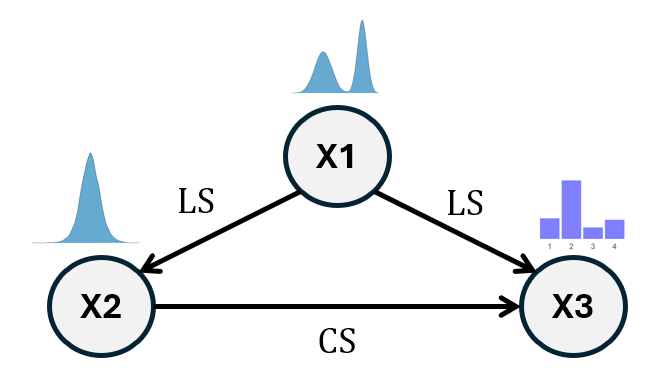
\includegraphics[width=0.28\textwidth]{img/exp1_DAG_MA.png}};
  \node (matrix) at (5, 0) {
    $\mathbf{MA} =
    \begin{bmatrix}
      0 & \text{LS} & \text{LS} \\
      0 & 0  & \text{CS} \\
      0 & 0  & 0
    \end{bmatrix}$
  };
  \draw[->, thick] (img.east) -- (matrix.west);
\end{tikzpicture}
\caption{Causal graph (left) and meta-adjacency matrix (right) for Experiment 1 (Section~\ref{ch:exp1}). The transformation function of $X_2$ depends on $X_1$ via a linear shift (LS). The transformation function of $X_3$ depends on $X_1$ via a linear shift (LS) and on $X_2$ via a complex shift (CS).}
\label{fig:dag_and_matrix}
\end{figure}

The variable $X_1$ is continuous and bimodally distributed, and acts as a source node in the DAG, i.e., it is not influenced by any other variable:

\[
X_1 = 
\begin{cases}
\mathcal{N}(0.25,\, 0.1^2) & \text{with probability } 0.5, \\
\mathcal{N}(0.73,\, 0.05^2) & \text{with probability } 0.5
\end{cases}
\]


    
The second variable, $X_2$, is continuous and linearly dependent on $X_1$ on the log-odds scale, with a true coefficient of $\beta_{12} = 2$. Its transformation function is 
\[
h(X_2 \mid X_1) = h_I(X_2) + \beta_{12} X_1,
\]
where the baseline transformation (i.e., intercept) of $X_2$ is $h_I(X_2) = 5 X_2$.

The third variable, $X_3$, is ordinal and depends on both $X_1$ (LS) and $X_2$ (CS). We define the complex shift induced by $X_2$ as $f(X_2) = 0.5 \cdot \exp(X_2)$, and specify the linear shift parameter for $X_1$ as $\beta_{13} = 0.2$. The transformation function for category $k$ of the ordinal variable $X_3$ with 4 levels ($K$) is thus defined by 
\[
h(X_{3,k} \mid X_1, X_2) = \vartheta_k + \beta_{13} X_1 + f(X_2),
\]
with cut-points $\vartheta_k \in \{-2,\, 0.42,\, 1.02\}$ defining the thresholds of the ordinal variable. We generated samples for $X_2$ and $X_3$ as described in Section~\ref{methods:sampling}, by first sampling a latent value from the standard logistic distribution and then determining the corresponding observation using the transformation function.

This simulation allows us to assess whether the TRAM-DAG model can correctly recover the functional forms of the conditional dependencies and the associated parameters (linear and complex).

\medskip

\textbf{Model:} Given the meta-adjacency matrix and the simulated observations, we construct a modular neural network based on the TRAM-DAG framework. The complex shift from $X_2$ to $X_3$ is modeled using a neural network with 4 hidden layers and 2 nodes per layer, as illustrated in Figure~\ref{fig:exp1_CS}. A total of 20,000 samples are generated according to the defined DGP to fit the model. We train the model for 400 epochs using the Adam optimizer \citep{kingma2015} with a learning rate of 0.005.


% include the figure for CS

\begin{figure}[H]
\centering
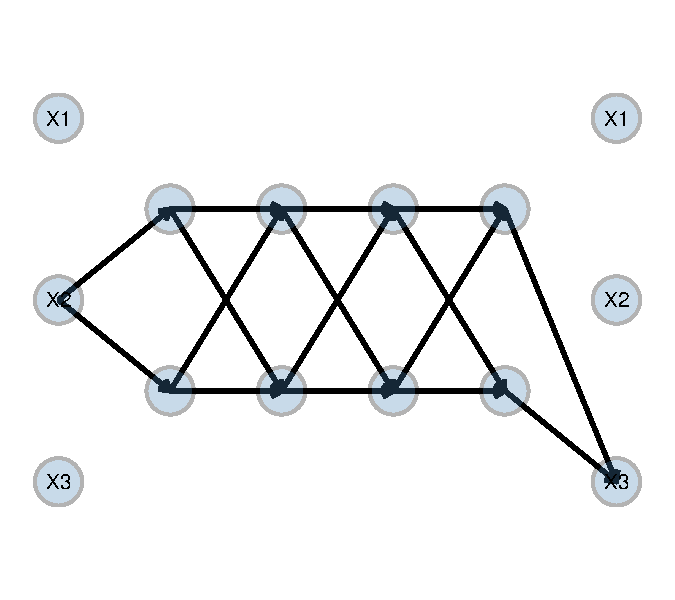
\includegraphics[width=0.5\linewidth]{img/exp1_CS.pdf}
\caption{Neural network architecture for the complex shift on $X_3$ from $X_2$ in Experiment 1 (Section~\ref{ch:exp1}). The complex shift is modeled by a neural network with 4 hidden layers of shape (2, 2, 2, 2), using non-linear activation functions (sigmoid).}
\label{fig:exp1_CS}
\end{figure}




\textbf{Model evaluation: } We compare the estimated intercepts, learned coefficients, and the complex shift to the true values used in the DGP. We also compare the sampled observational and interventional distributions to the true distributions. For the counterfactual queries, we show the estimated counterfactual values for $X_2$ under an intervention on $X_1$ at a specific value, and compare these to the true counterfactual outcomes.




\subsection{Results}



We evaluate whether TRAM-DAGs can recover the structural equations and distributions used in the data-generating process described in Section~\ref{sec:methods_experiment1}. Below, we present the training process and inspect the estimated parameters, distributions, and counterfactual predictions.

Figure \ref{fig:exp1_loss_parameters} shows the loss and the estimated parameters for the linear shifts over epochs during training. The loss was minimized during training and the estimated parameters $\beta_{12}$ and $\beta_{13}$ converged to the true values used in the DGP. The linear shift parameters are the interpretable part of the model (log-odds ratios). From the fitted model, we generated samples from the observational distribution, as shown in Figure \ref{fig:exp1_observational_distribution}. The TRAM-DAG can recover the observational distribution as its samples align with the data that was used to fit the model. Then we drew samples from the interventional distribution, where $X_2 = 1$ is fixed, as shown in Figure \ref{fig:exp1_interventional_distribution}. Fixing $X_2$ leads to a distributional change in $X_3$, which was also captured by the model. The TRAM-DAG learns the linear shifts ($\beta_{12}$, $\beta_{13}$) and the complex shift $f(X_2)$, which are shown in Figure \ref{fig:exp1_shifts}. Figure~\ref{fig:exp1_intercepts} presents the intercepts learned for each of the nodes. For comparison, we added the estimated intercept functions from the Continuous Outcome Logistic Regression (Colr() function from the \texttt{tram} \texttt{R}-package \citep{hothorn2018}) for $X_1$ and $X_2$, and the true values used in the DGP for the ordinal variable $X_3$ (three cut-points for the four levels). Since the transformation functions for $X_1$ and $X_2$ contain no complex terms, they match the default form used in Colr(). Finally, Figure~\ref{fig:exp1_counterfactuals} shows the counterfactuals for $X_2$ estimated by the TRAM-DAG for varying values of $X_1$. The counterfactuals are the predicted values of $X_2$ had $X_1$ taken other values instead of the initially observed one. 

\begin{figure}[htbp]
\centering
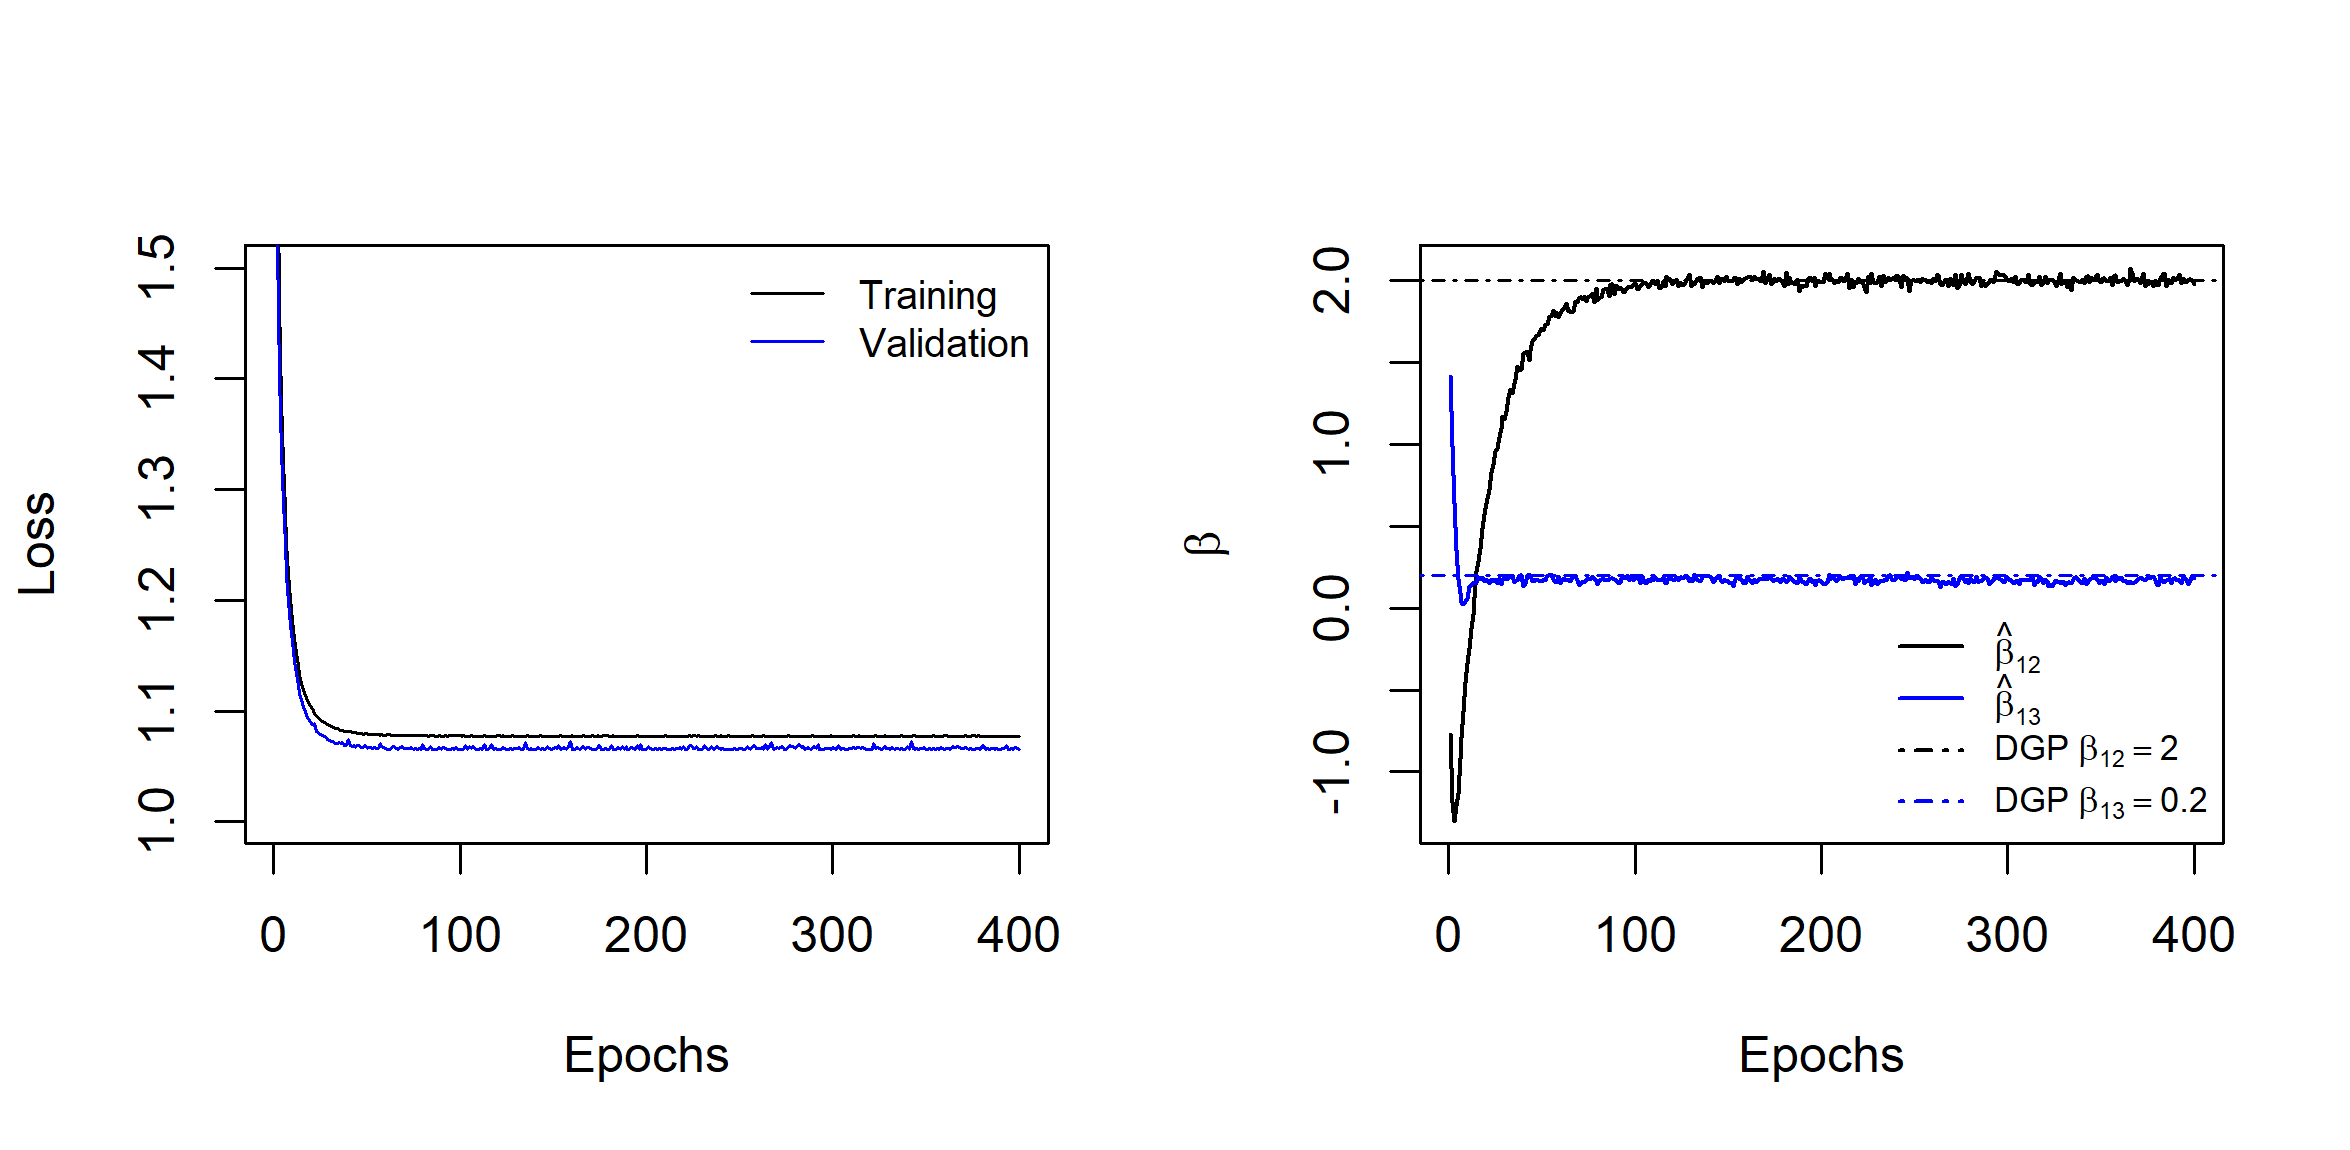
\includegraphics[width=0.9\textwidth]{img/exp1_loss_parameters.png}
\caption{TRAM-DAG model fitting over 400 epochs for Experiment 1. Left: loss functions on the training and validation sets; Right: estimated parameters (betas) for the linear shift components over epochs. The estimates converge to the true values used in the DGP.}
\label{fig:exp1_loss_parameters}
\end{figure}



\begin{figure}[htbp]
\centering
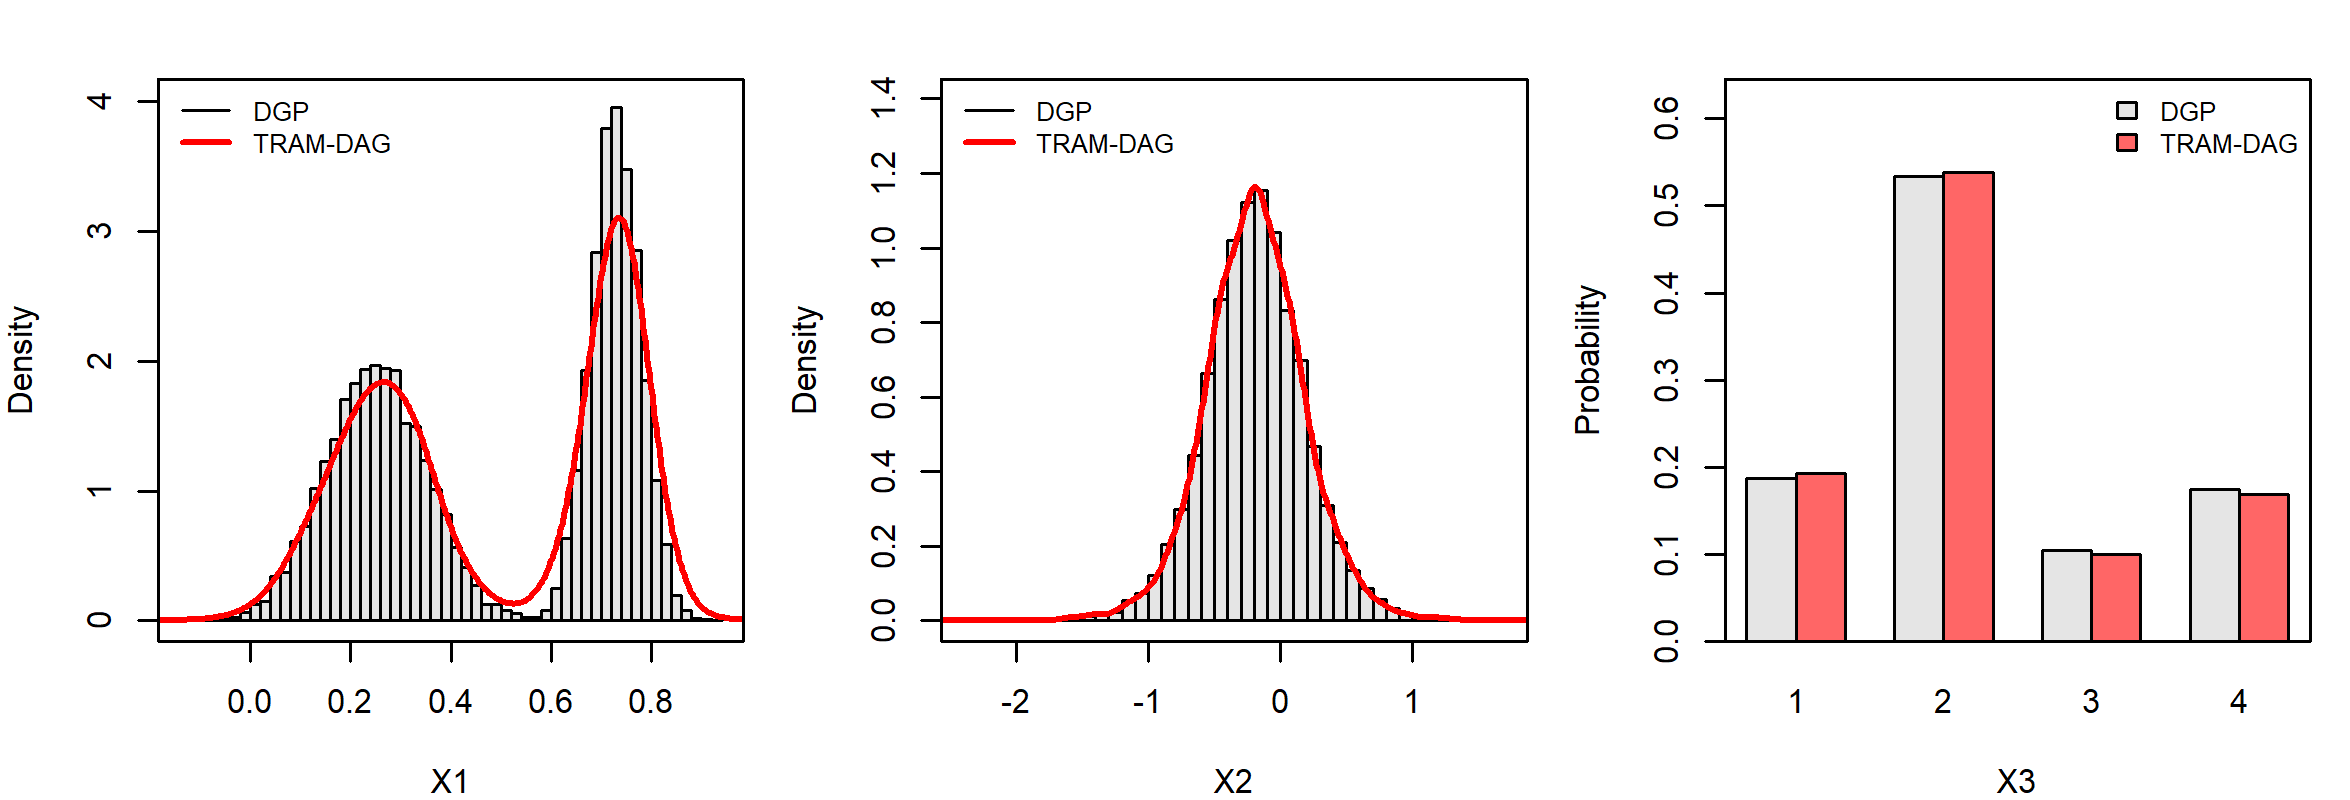
\includegraphics[width=0.9\textwidth]{img/exp1_observational_distribution.png}
\caption{Samples generated by the TRAM-DAG from the learned observational distribution, compared to the true observations from the DGP.}
\label{fig:exp1_observational_distribution}
\end{figure}




\begin{figure}[htbp]
\centering
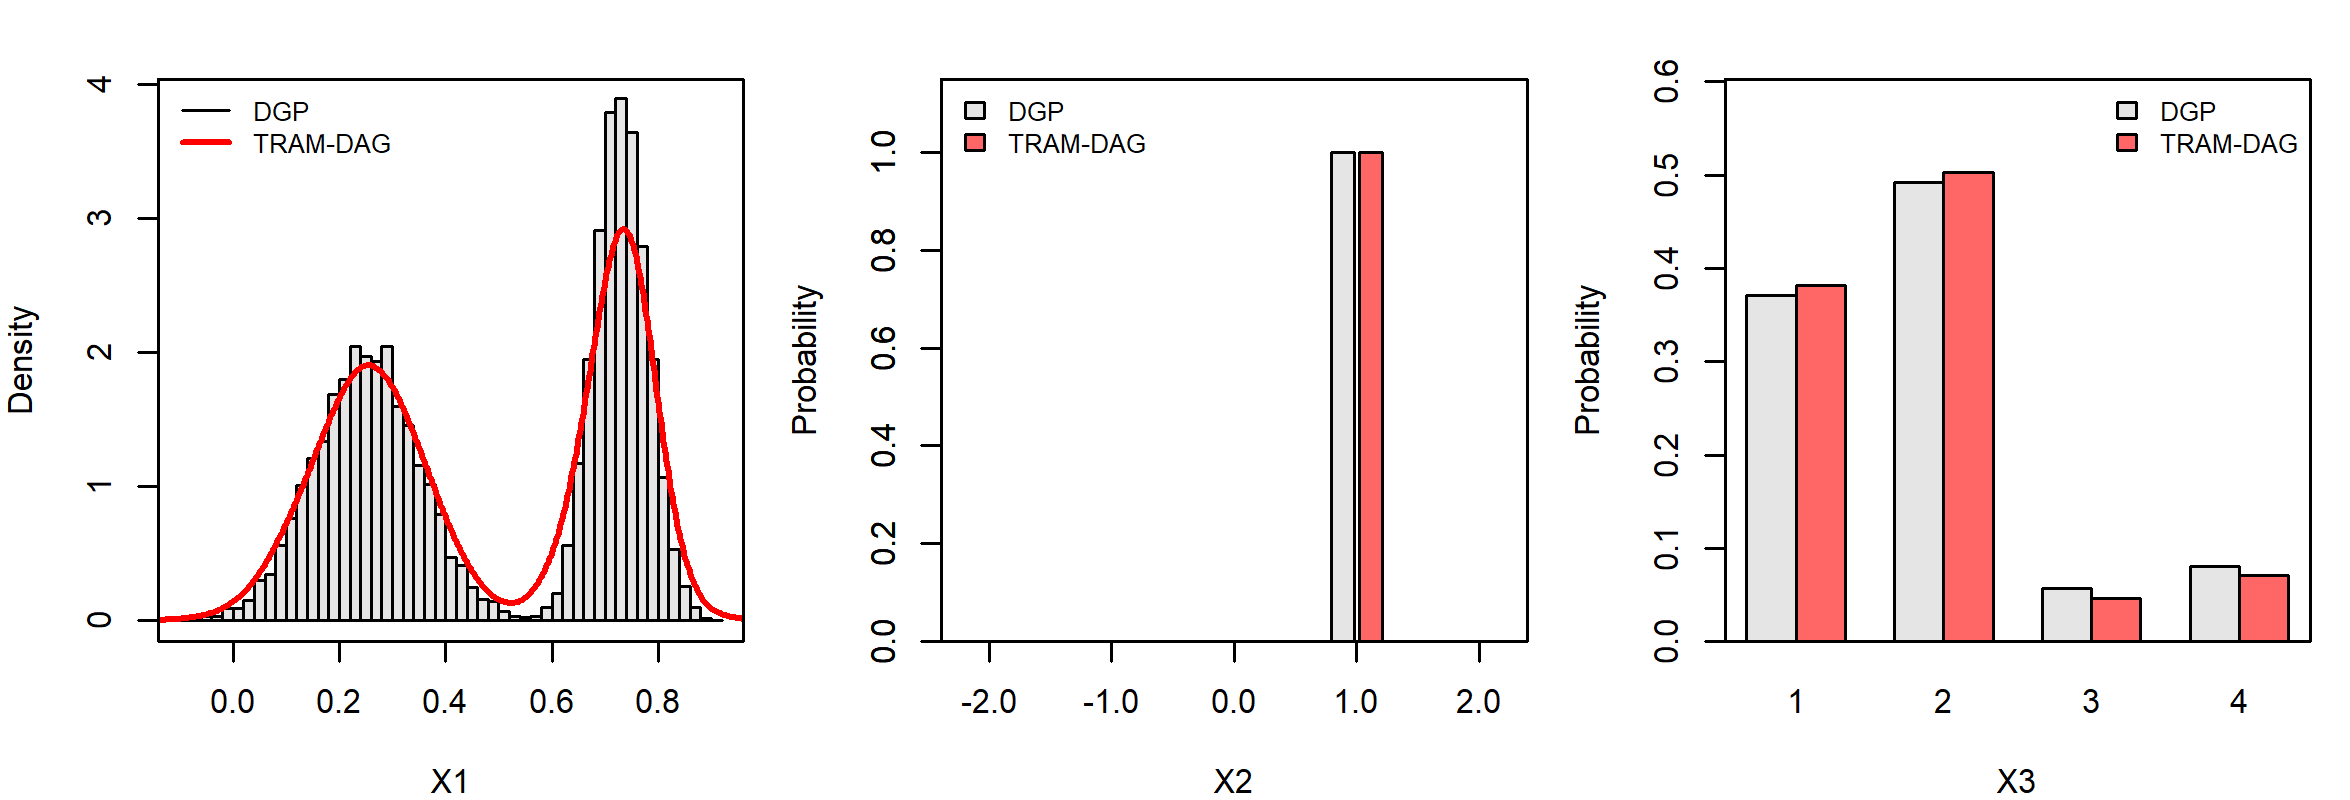
\includegraphics[width=0.9\textwidth]{img/exp1_interventional_distribution.png}
\caption{Samples generated by the TRAM-DAG compared to the true observations from the interventional distribution of the DGP, where $X_2 = 1$ is fixed. According to the DAG, this intervention induces a distributional change in $X_3$.}
\label{fig:exp1_interventional_distribution}
\end{figure}



\begin{figure}[htbp]
\centering
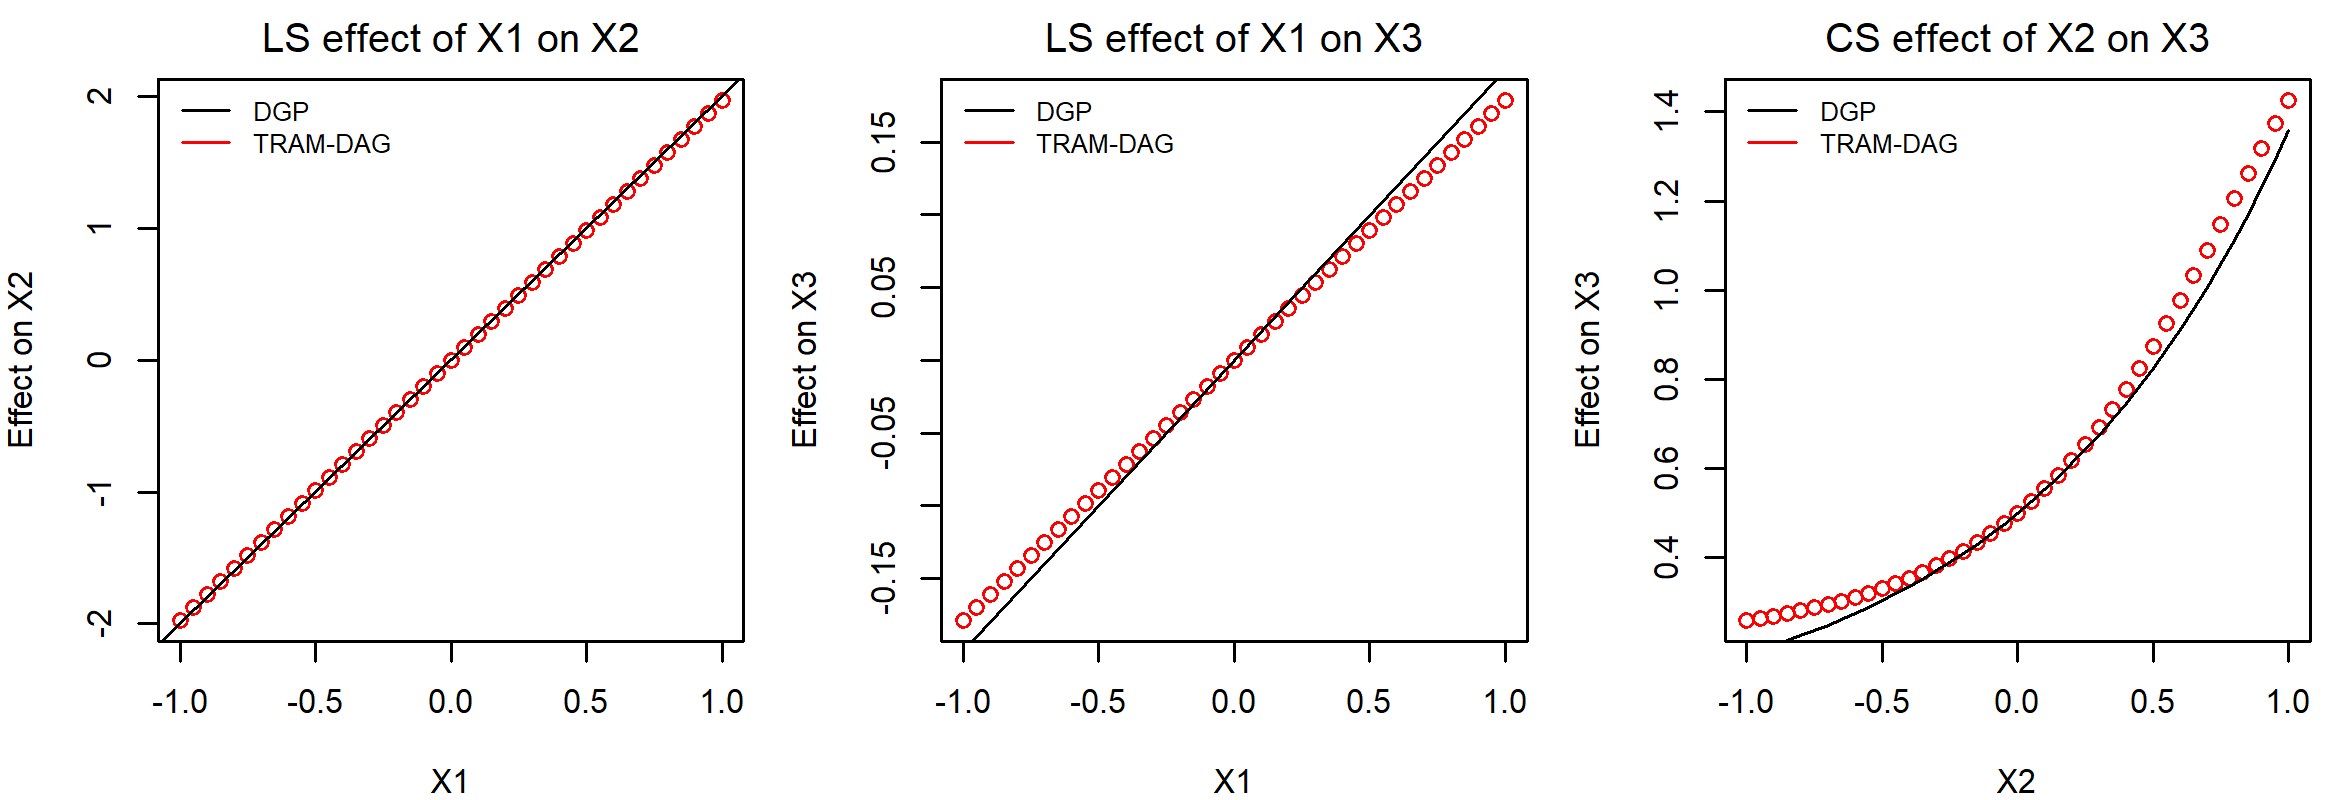
\includegraphics[width=0.9\textwidth]{img/exp1_LS_CS.png}
\caption{Linear and complex shifts learned by the TRAM-DAG. Left: LS($X_1$) on $X_2$; Middle: LS($X_1$) on $X_3$; Right: CS($X_2$) on $X_3$. For visualization, we subtracted $\delta_0 = \text{CS}(0) - f(0)$ from the estimated complex shift CS($X_2$) to align it with the true shift function $f(X_2)$ from the DGP.}
\label{fig:exp1_shifts}
\end{figure}



\begin{figure}[htbp]
\centering
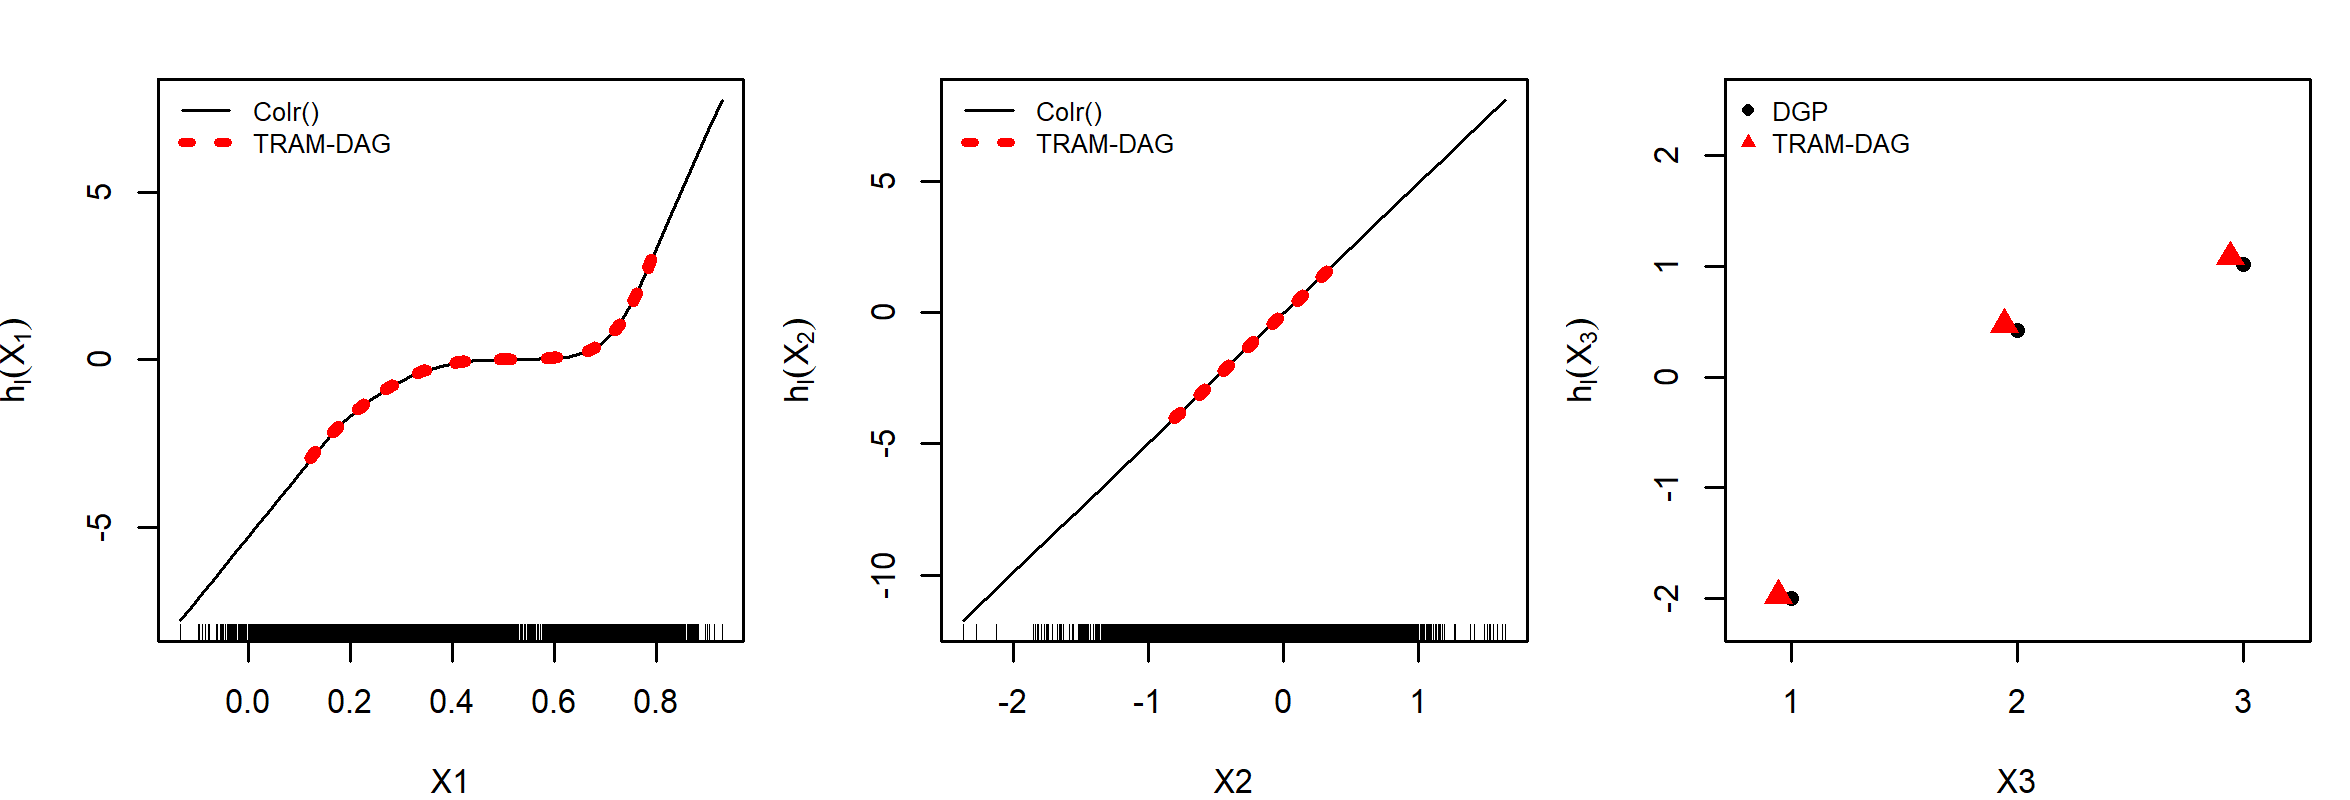
\includegraphics[width=0.9\textwidth]{img/exp1_baseline_trafo.png}
\caption{Intercepts learned for each of the nodes, along with the estimates from the \texttt{Colr()} function for the continuous variables and the true values from the DGP for the ordinal variable $X_3$. Left: Smooth baseline transformation function for continuous $X_1$; Middle: Smooth baseline transformation function for continuous $X_2$; Right: Cut-points as the baseline transformation function for ordinal $X_3$. For the last plot, we added $\delta_0 = \text{CS}(0) - f(0)$ to the estimated cut-offs to make them comparable to the true parameters from the DGP.}
\label{fig:exp1_intercepts}
\end{figure}




\begin{figure}[htbp]
\centering
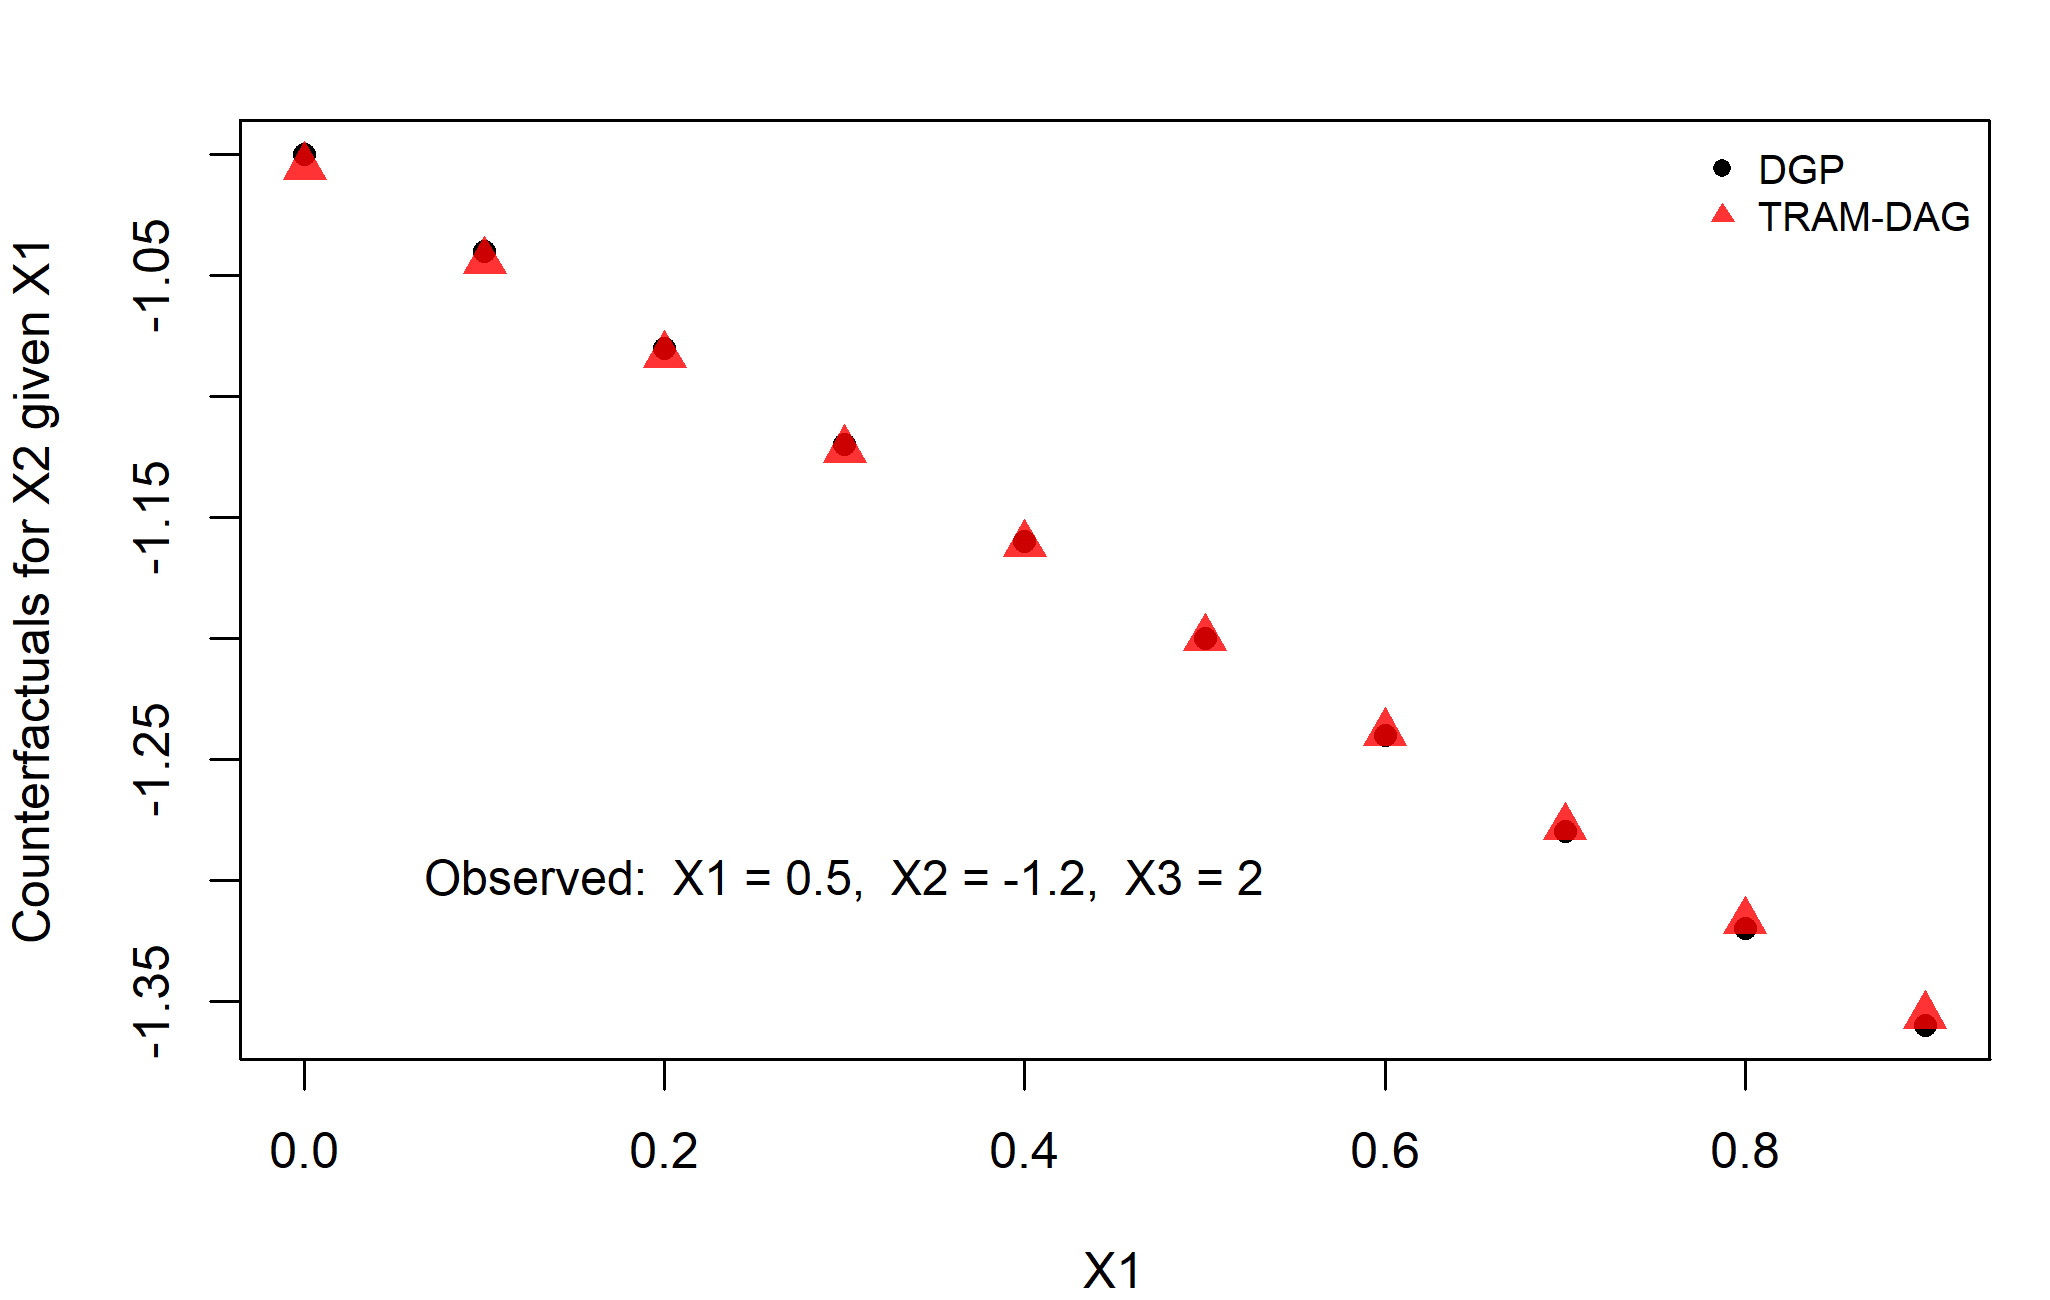
\includegraphics[width=0.9\textwidth]{img/exp1_counterfactuals.png}

\caption{Counterfactuals for $X_2$ estimated with the TRAM-DAG for varying values of $X_1$. We assumed the observed values $X_1 = 0.5$, $X_2 = -1.2$, and $X_3 = 2$, and determined the counterfactual values of $X_2$ had $X_1$ taken different values instead of the actually observed one. This illustrates how the model estimates alternative outcomes under hypothetical interventions on $X_1$.}
\label{fig:exp1_counterfactuals}
\end{figure}



% enforce that starts after all floats have been displayed
\FloatBarrier

\subsection{Discussion of Experiment 1}

The results show that the TRAM-DAG framework can accurately recover the underlying causal relationships from data, including both linear and nonlinear (complex) relationships. This enabled the model to generate observational and interventional distributions (Figures~\ref{fig:exp1_observational_distribution} and~\ref{fig:exp1_interventional_distribution}) that closely matched the true ones, and produce valid counterfactual predictions (Figure~\ref{fig:exp1_counterfactuals}).

This experiment provides a simple proof of concept for the flexibility and generative capability of TRAM-DAGs. By incorporating both interpretable (e.g., linear shifts) and flexible (e.g., complex shift) components, the model is able to capture a range of causal mechanisms -- provided that the true DAG is known and data is generated accordingly.


% \section{Discussion}
% 
% 
% The results demonstrate that the TRAM-DAG framework can learn the true parameters and both linear and complex shifts from the data, enabling it to act as a generative model for predicting interventions and counterfactuals. It successfully reproduced observational and interventional distributions and predicted correct counterfactual outcomes.
% 
% This experiment serves as a small proof of concept that TRAM-DAGs can be specified flexibly, with both interpretable and complex components, to capture causal relationships of varying complexity when the true DAG is known and the data is generated accordingly.








% LaTeX file for Chapter Exp2






\section{Experiment 2: ITE on International Stroke Trial (IST)} \label{ch:exp2}





\subsection{Motivation}


% describe the data of stroke trial https://pubmed.ncbi.nlm.nih.gov/9174558/
% Results on IST trial with the interpretation in the discussion part.

%  here the authors made the IST database available and described the trial, we downloaded the CSV
% https://trialsjournal.biomedcentral.com/articles/10.1186/1745-6215-12-101 


% Results: The IST dataset includes data on 19 435 patients with acute stroke, with 99% complete follow-up. Over 26.4% patients were aged over 80 years at study entry. Background stroke care was limited and none of the patients received thrombolytic therapy.
% 
% 
\citet{chen2025} evaluated multiple causal ML methods on the International Stroke Trial (IST), to estimate the individualized treatment effects (ITEs). They demonstrated that none of the applied ML methods generalized well, as performance on the test data differed significantly from the training data on the chosen evaluation metrics.
In this experiment, we replicate the analysis on the same data by applying three causal ML methods for ITE estimation, to investigate whether we obtain similar results as the authors.


\subsection{Setup} \label{sec:methods_experiment2}



\textbf{Data:} The International Stroke Trial was a large, randomized controlled trial conducted in the 1990s to assess the efficacy and safety of early antithrombotic treatment in patients with acute ischemic stroke \citep{IST1997}. Using a 2x2 factorial design, 19,435 patients across 36 countries were randomized within 48 hours of symptom onset to receive aspirin, subcutaneous heparin, both, or neither. Patients allocated to aspirin (300 mg daily for 14 days) had a 6-month death or dependency rate of 62.2\%, compared to 63.5\% in the control group not receiving aspirin, corresponding to a statistically significant absolute risk reduction after adjustment for baseline prognosis (1.4\%, p = 0.03). The authors stated that there was no interaction between aspirin and heparin in the main outcomes. In this thesis, we focus exclusively on the aspirin vs. no aspirin comparison and the outcome of death or dependency at 6 months after stroke.

The dataset used in this experiment was made publicly available by \citet{sandercock2011} and contains individual-level data, including baseline covariates assessed at randomization, treatment allocation, and 6-month outcomes, with a follow-up rate of 99\%.

We used the same data pre-processing steps as \citet{chen2025} to ensure comparability of results. 5.9\% of individuals had incomplete data and were removed from the dataset. We used 2/3 of the data for fitting the models and 1/3 as a hold out test set. The final dataset included 21 baseline variables recorded at randomization: aspirin allocation (treatment), age, delay between stroke and randomization (in hours), systolic blood pressure, sex, CT performed before randomization, visible infarct on CT, atrial fibrillation, aspirin use within 3 days prior to randomization, and presence or absence of neurological deficits (including face, arm/hand, leg/foot deficits, dysphasia, hemianopia, visuospatial disorder, brainstem or cerebellar signs, and other neurological deficits), as well as consciousness level, stroke subtype, and geographical region. The outcome variable was death or dependence at 6 months.


\medskip

\textbf{Models for ITE estimation: } The aim is to estimate the ITE (Equation~\ref{eq:ITE_binary}) based on baseline characteristics. As a benchmark, we apply a T-learner logistic regression (following \citet{chen2025}, using the \texttt{stats} package). As a more complex model, we apply a T-learner tuned random forest (using the \texttt{comets} package \citep{comets}), which tunes the number of variables considered for splitting at each node (\texttt{mtry}) and the maximum tree depth (\texttt{max.depth}) using out-of-bag error, with 500 trees. Additionally, we apply an S-learner TRAM-DAG. For the random forest and TRAM-DAG based methods, we additionally scale numerical and dummy encode categorical covariates prior to model training. The transformation function of the outcome is modelled by a complex intercept $h(Y \mid T, \mathbf{X}) = CI(T, \mathbf{X})$, with 4 hidden layers of shape (20, 10, 10, 2). This architecture allows for interaction between the treatment and covariates. Furthermore, batch normalization, ReLU activation, and dropout (0.1) are applied to prevent overfitting and stabilize learning. A validation set comprising 20\% of the training data is used to select the model with the lowest out-of-sample negative log-likelihood (Equation~\ref{eq:nll_tram}), while the test set remains untouched for final evaluation. 

Since the IST is a randomized controlled trial, the full potential of TRAM-DAGs -- designed primarily for use in observational settings -- is not required here, as only the outcome needs to be modeled as a function of baseline patient characteristics. However, applying TRAM-DAGs in this context still allows us to assess its predictive performance and ability to flexibly model interactions between variables.



\medskip

\textbf{Model evaluation: } For validation, since the ground truth is not known, we first rely on calibration plots to assess the general prediction power for the probabilities. Second, we predict the potential outcomes with the trained models to estimate the ITE on the training and test set in terms of the risk difference (see Equation~\ref{eq:ITE_binary}). For visual validation, we show the densities of the estimated ITEs on both datasets, and the ITE-ATE plots to assess whether the estimated ITEs align with the observed outcomes.










% possible example of unobserved interaction:
% An example could be the psychological condition of a patient which might also affect how the treatment works, this is not a confounder but an effect modifier, and i would assume that this variable is rarely recorede or measured.




\subsection{Results} \label{sec:results_experiment2}


In this section, we present the results of the ITE estimation on the International Stroke Trial (IST) dataset. 

The observed average treatment effect (ATE), defined as $P(Y=1|T=1) - P(Y=1|T=0)$, was -2.4\% absolute risk reduction on the training set, with a 95\% confidence interval from -4.1\% to -0.6\%. The interval was computed using the Wald method for risk differences, with standard error $\sqrt{p_1 (1 - p_1)/n_1 + p_0 (1 - p_0)/n_0}$
, where $p_1$ and $p_0$ are the event rates in the treated and control groups. On the test set, the observed treatment effect was -0.1\%, with a 95\% confidence interval from -2.6\% to 2.3\%. 

To estimate ITEs (Equation~\ref{eq:ITE_binary}), we applied three models: a T-learner logistic regression, a T-learner tuned random forest, and an S-learner TRAM-DAG. The results for each model are shown in terms of (1) the density of predicted ITEs, and (2) ITE-ATE plots, which display the empirical risk difference within subgroups of estimated ITEs, including 95\% confidence intervals. Results are presented in Figures~\ref{fig:IST_density_ITE_ATE_glm_tlearner} (logistic regression), \ref{fig:IST_density_ITE_ATE_tuned_rf} (random forest), and~\ref{fig:IST_density_ITE_ATE_TRAM_DAG} (TRAM-DAG). Additionally, calibration plots are provided in Appendix~\ref{sec:calibrations_experiment2}, Figures \ref{fig:calibration_IST_glm} - \ref{fig:calibration_IST_TRAM_DAG}. 

% The ITEs were estimated using three different models, and the results are shown in terms of the density of predicted ITEs and the ITE-ATE plots for risk difference per estimated ITE subgroup, including 95\% confidence intervals: T-learner logistic regression (see results in Figure~\ref{fig:IST_density_ITE_ATE_glm_tlearner}), T-learner tuned random forest (see results in Figure~\ref{fig:IST_density_ITE_ATE_tuned_rf}), and S-learner TRAM-DAG (see results in Figure~\ref{fig:IST_density_ITE_ATE_TRAM_DAG}). 

The estimated average treatment effect on the test set, calculated as $\text{ATE}_\text{pred}=\text{mean}(\text{ITE}_\text{pred})$, was -2.5\% for the T-learner logistic regression, -2.2\% for the T-learner tuned random forest, and -3.1\% for the S-learner TRAM-DAG.  




\begin{figure}[htbp]
\centering
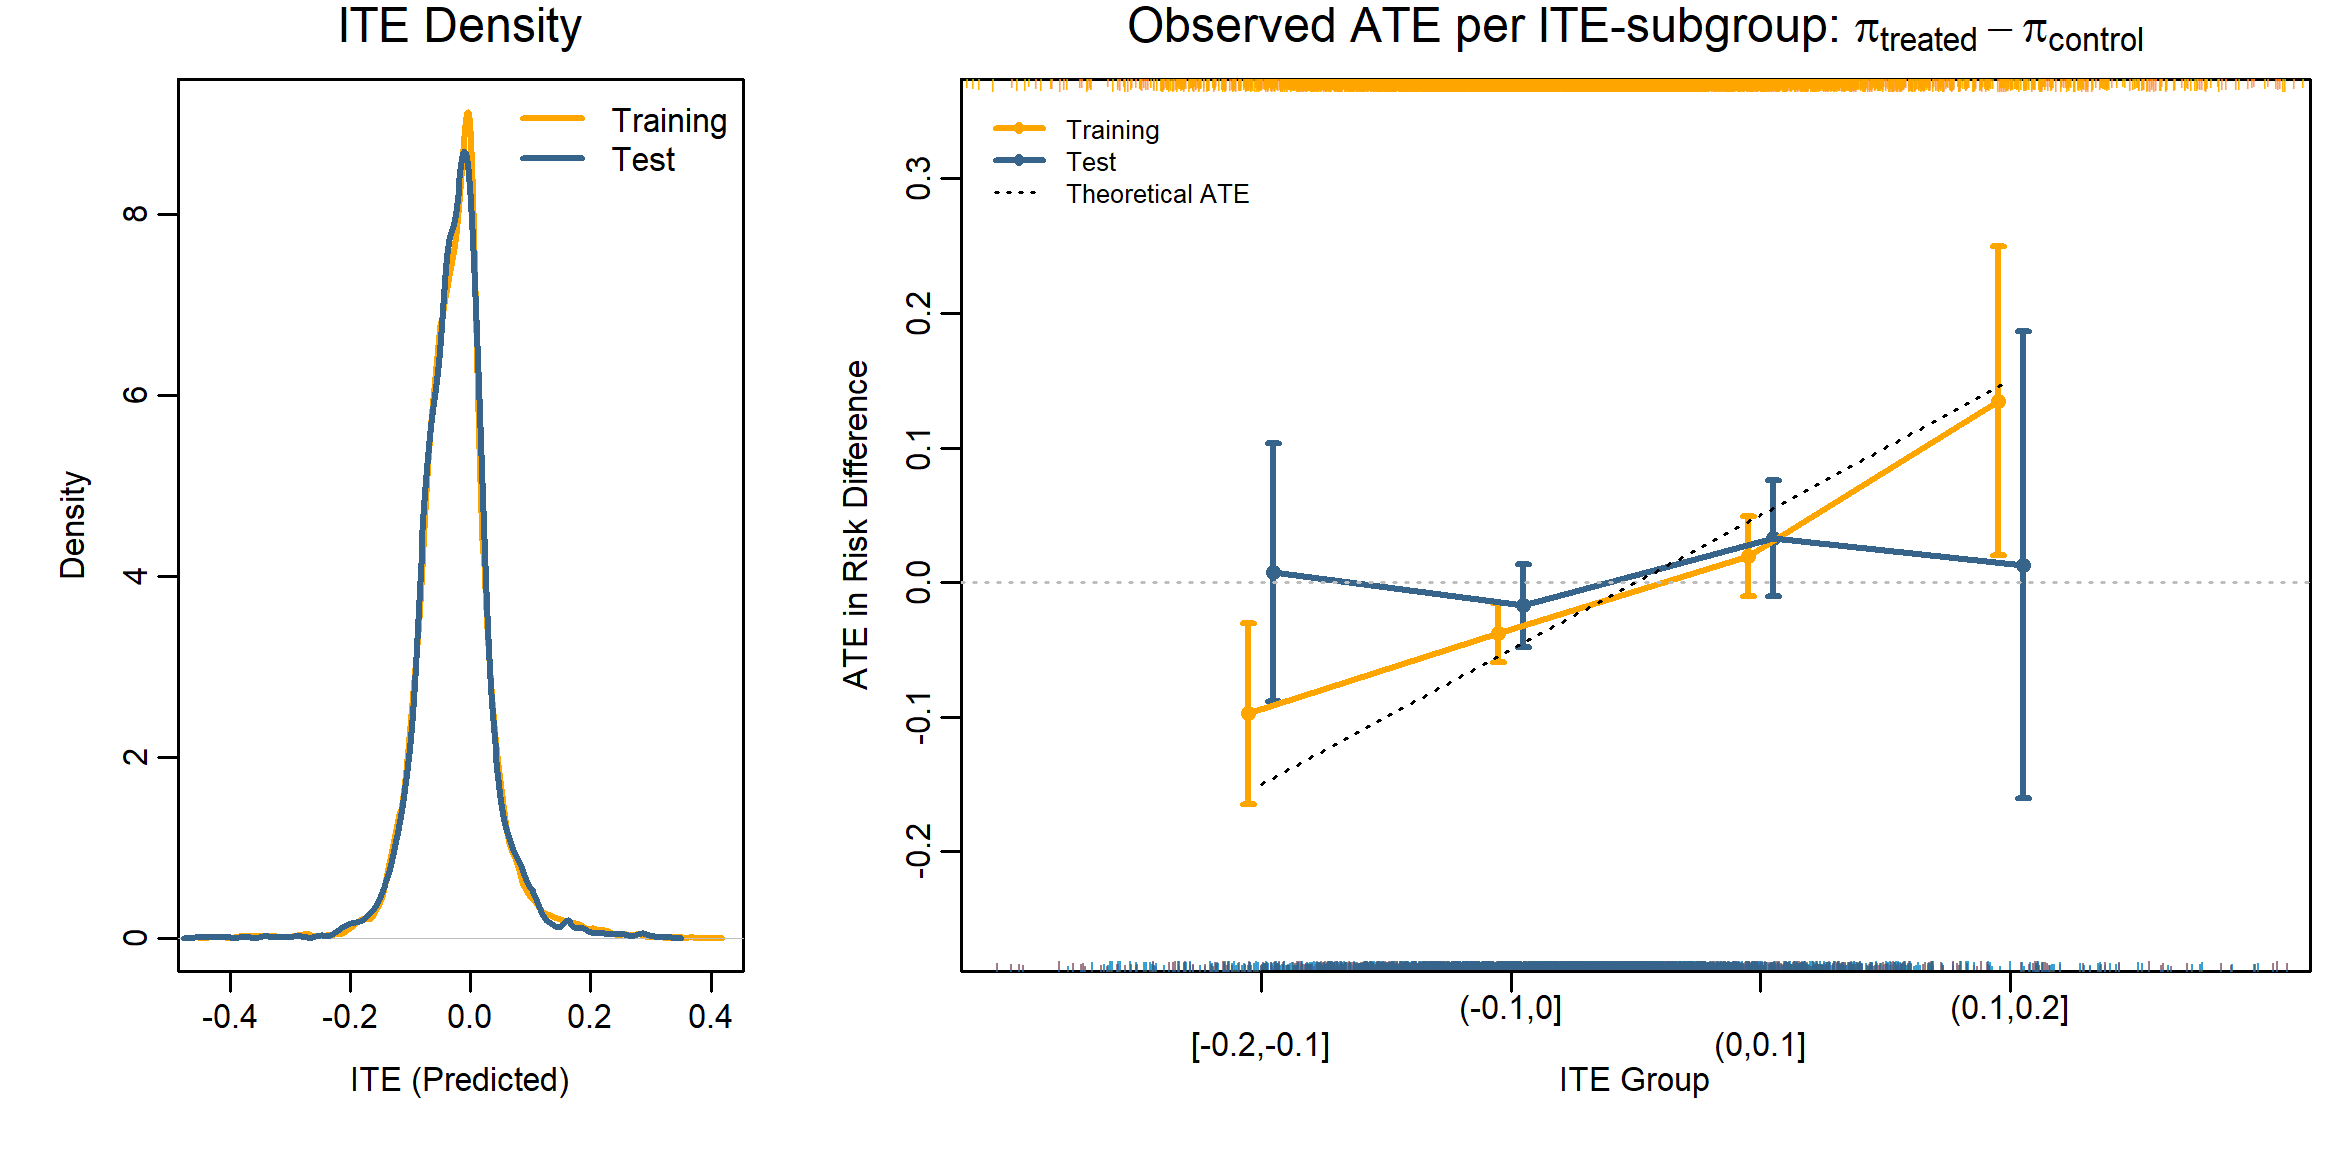
\includegraphics[width=0.9\textwidth]{img/results_IST/glm_tlearner_density_ITE_ATE.png}
\caption{Results for the International Stroke Trial (IST) using the T-learner logistic regression. Left: density of predicted ITEs in the training and test sets; Right: observed ATE in terms of risk difference per estimated ITE subgroup.}
\label{fig:IST_density_ITE_ATE_glm_tlearner}
\end{figure}



\begin{figure}[htbp]
\centering
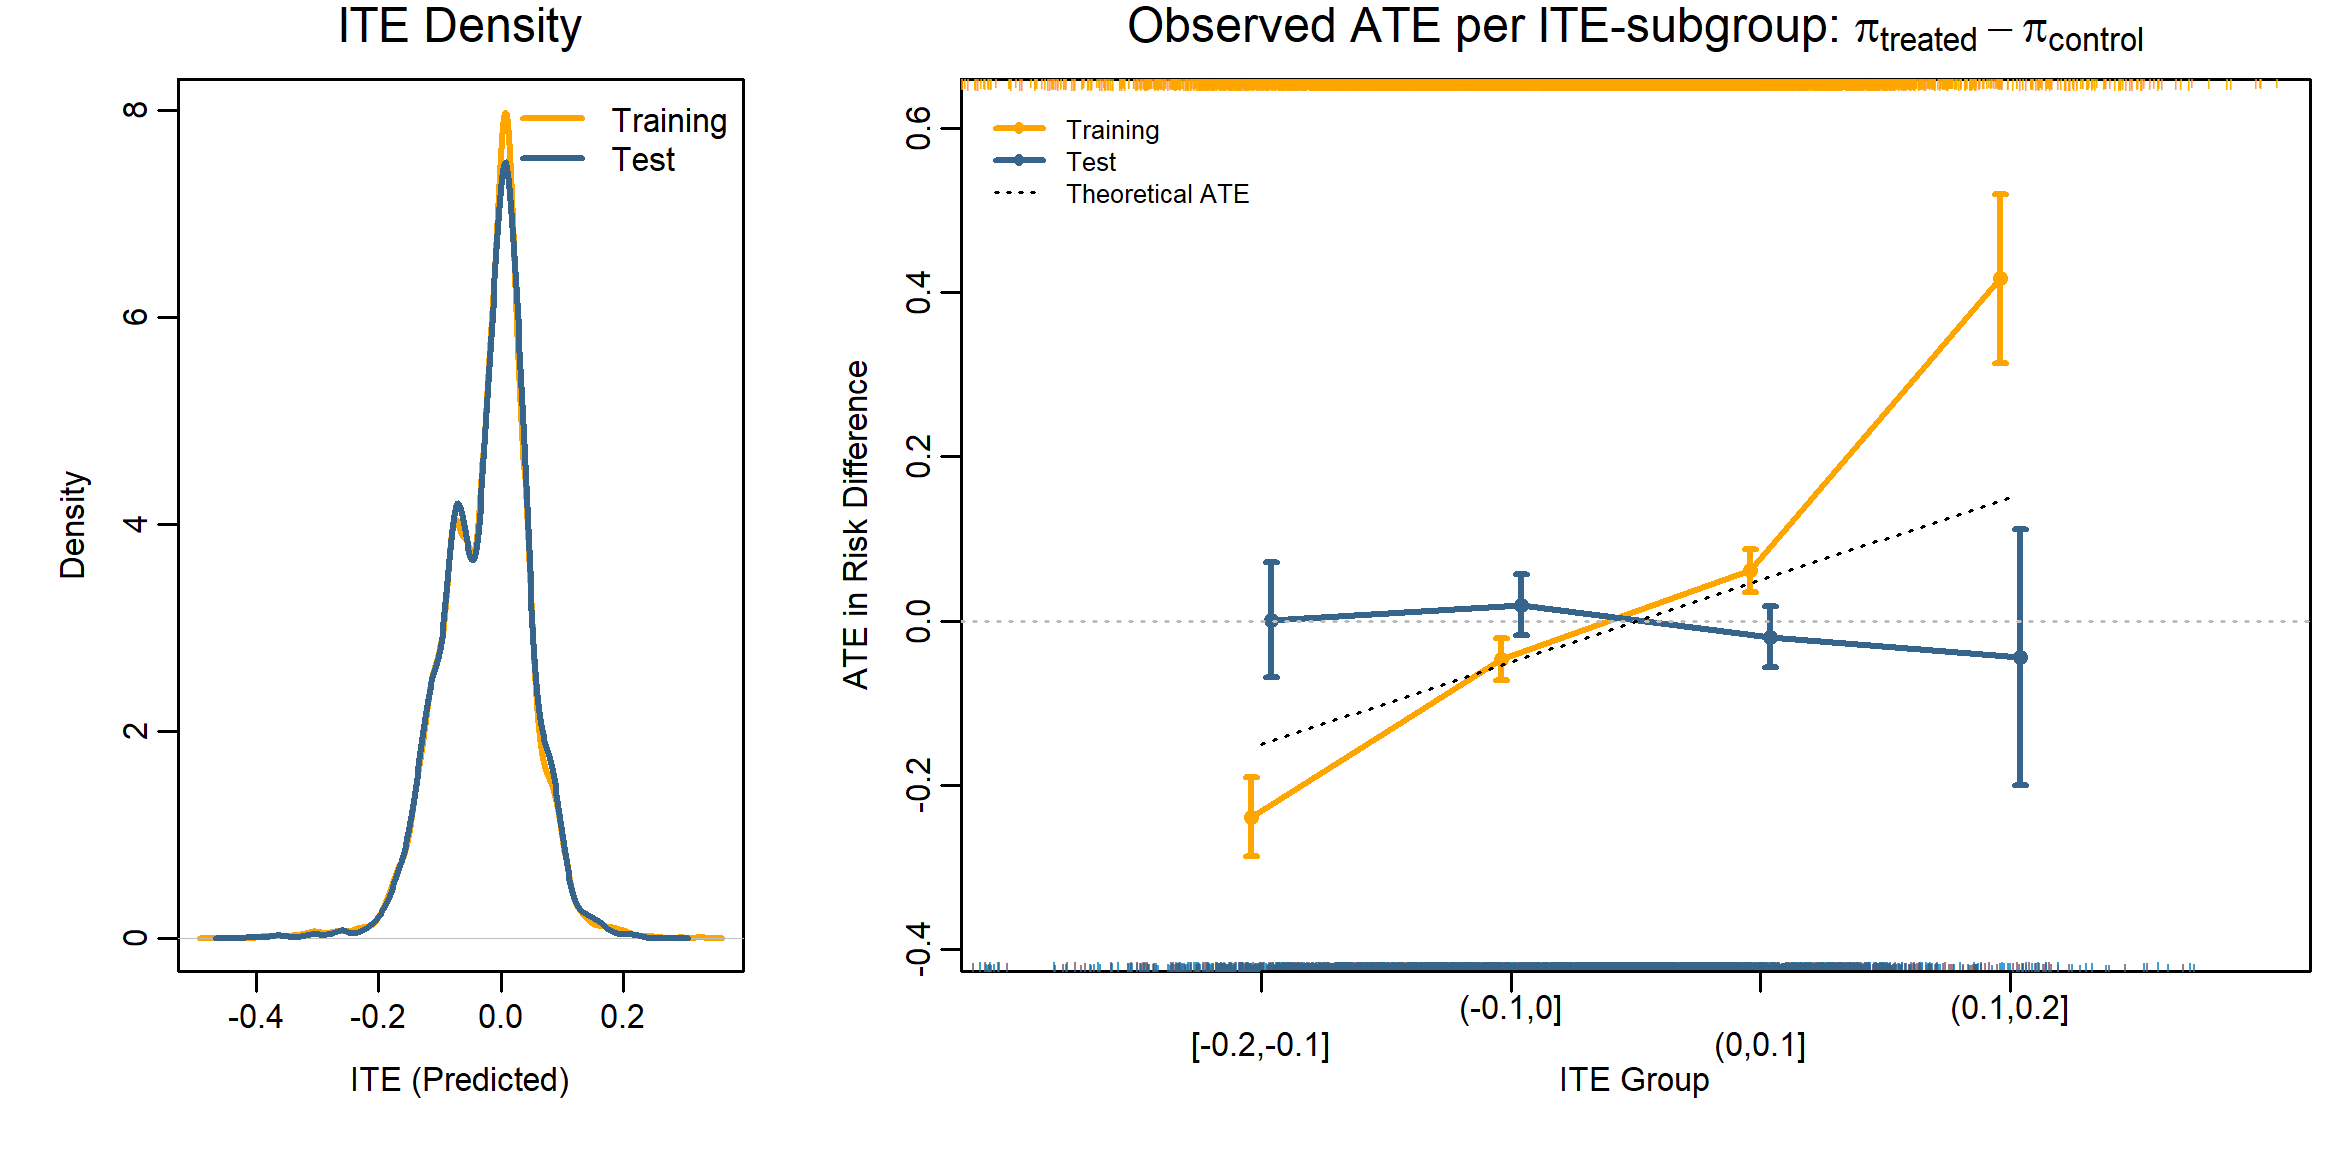
\includegraphics[width=0.9\textwidth]{img/results_IST/IST_tuned_rf_tlearner_density_ITE_ATE.png}
\caption{Results for the International Stroke Trial (IST) using the T-learner tuned random forest. Left: density of predicted ITEs in the training and test sets; Right: observed ATE in terms of risk difference per estimated ITE subgroup.}
\label{fig:IST_density_ITE_ATE_tuned_rf}
\end{figure}




\begin{figure}[htbp]
\centering
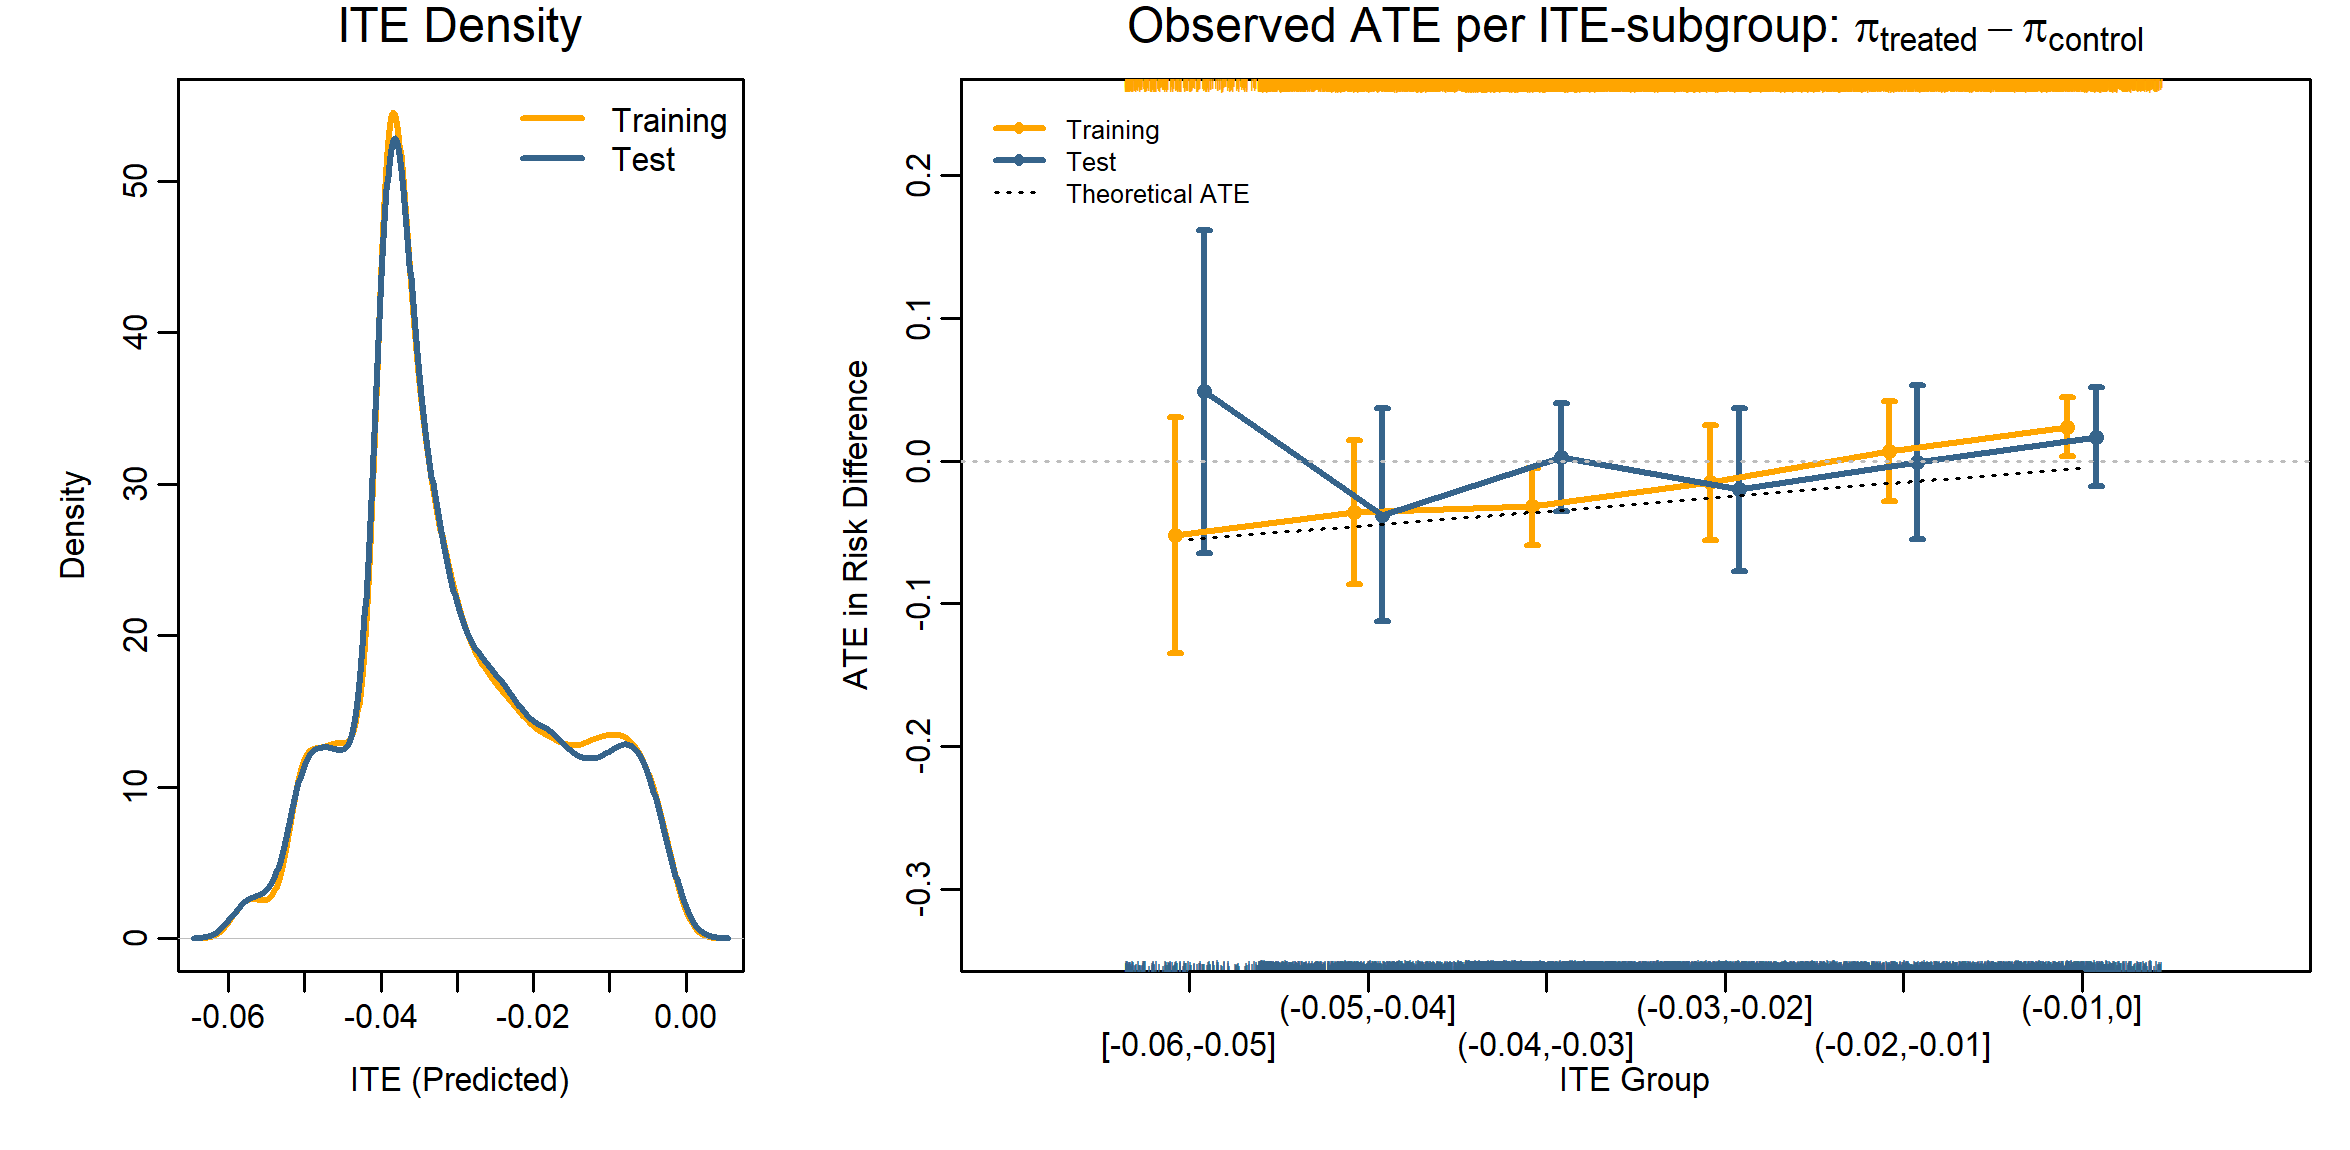
\includegraphics[width=0.9\textwidth]{img/results_IST/IST_TRAM_DAG_slearner_density_ITE_ATE.png}
\caption{Results for the International Stroke Trial (IST) using the S-learner TRAM-DAG. Left: density of predicted ITEs in the training and test sets; Right: observed ATE in terms of risk difference per estimated ITE subgroup.}
\label{fig:IST_density_ITE_ATE_TRAM_DAG}
\end{figure}


enforce that starts after all floats have been displayed
\FloatBarrier


\subsection{Discussion of Experiment 2}

We observed similar results to those reported by \citet{chen2025} when estimating ITEs on the International Stroke Trial dataset across all three models: the T-learner logistic regression, the T-learner tuned random forest, and the S-learner TRAM-DAG. The logistic model showed moderate discrimination in the training set, which did not generalize to the test set, as illustrated by the ITE-ATE plot in Figure~\ref{fig:IST_density_ITE_ATE_glm_tlearner}. The tuned random forest model showed stronger discrimination in the training set but similarly failed to generalize to the test set (see Figure~\ref{fig:IST_density_ITE_ATE_tuned_rf}). In contrast, the S-learner TRAM-DAG estimated less heterogeneity than the other two models, as shown in the density plot in Figure~\ref{fig:IST_density_ITE_ATE_TRAM_DAG}, resulting in weak discrimination in both the training and test sets, visible in the corresponding ITE-ATE plot. For all three models, the confidence intervals in the ITE-ATE plots on the test set included the zero line, suggesting no significant effect in any of the estimated ITE subgroups.

\medskip


Poor calibration does not appear to explain the limited ITE performance, as calibration on the test set was good, as shown in Appendix~\ref{sec:calibrations_experiment2}, Figures~\ref{fig:calibration_IST_glm}-\ref{fig:calibration_IST_TRAM_DAG}. However, since the ground truth is unknown, it remains unclear whether the models fail to detect true treatment effect heterogeneity, or whether the heterogeneity is too small, or driven by unobserved effect modifiers. We investigate these possibilities further in Experiment 3, Section~\ref{ch:experiment3}.






% LaTeX file for Chapter Exp3




\section{Experiment 3: ITE model robustness in RCTs (simulation)} \label{ch:experiment3}




\subsection{Motivation}

In this section, we perform a simulation study to estimate ITEs using different models in an RCT setting under various scenarios. The aim is to identify conditions under which ITE estimation fails, and whether such failure is model-agnostic -- i.e., driven by external factors such as unobserved covariates or the strength of the treatment effect, rather than by the model class itself. This may provide insight into why ITE estimation can fail in real-world applications, as demonstrated by \citet{chen2025} on the IST dataset and replicated in our own work in Experiment 2 (Section~\ref{ch:exp2}). 


\subsection{Setup} \label{sec:methods_experiment3}

The simulation is based on a data-generating process (DGP) that resembles an RCT. We assume a binary outcome and a set of covariates that influence the outcome. There may also be treatment-covariate interactions that are responsible for heterogeneity in the treatment effect.

\medskip

\textbf{Data-generating process:} Data is generated similarly to the approach proposed by \citet{hoogland2021}. The binary treatment ($T$) is sampled from a Bernoulli distribution with probability 0.5. The five covariates ($\mathbf{X}$), representing patient-specific characteristics at baseline, are drawn from a multivariate standard normal distribution with a compound symmetric covariance matrix ($\rho=0.1$). The binary outcome ($Y$) is sampled from a Bernoulli distribution with probability $P(Y_i = 1 \mid  \mathbf{X} = \mathbf{x_i}, T = t_i) = \text{logit}^{-1} \left(\beta_0 + \beta_T t_i + \boldsymbol{\beta}_X^\top \mathbf{x_i} + t_i \cdot \boldsymbol{\beta}_{TX}^\top \mathbf{x_{TX,i}} \right)$, where $i$ denotes the patient index, and $\mathbf{x}_{TX,i}$ denotes the subset of covariates that interact with the treatment.

The simulated datasets are generated under three scenarios, where coefficients are set to different values or not all variables are observed. In Scenario 3.1, the coefficients are: $\beta_0 = 0.45$ (intercept), $\beta_T = -0.85$ (direct treatment effect), $\boldsymbol{\beta}_X = (-0.5, 0.8, 0.2, 0.6, -0.4)$ (direct covariate effects), and $\boldsymbol{\beta}_{TX} = (0.9, 0.1)$ (interaction effects between treatment and covariates $X_1$ and $X_2$ on the outcome). In Scenario 3.2, the same coefficients are used, but the covariate $X_1$, which is responsible for a large portion of the heterogeneity, is not observed in the final dataset. This is expected to cause difficulties in estimating the ITE. In Scenario 3.3, the coefficients for the direct treatment and interaction effects are set to $\beta_T = -0.05$ and $\boldsymbol{\beta}_{TX} = (-0.01, 0.03)$ to represent a weak treatment effect and low heterogeneity. All other coefficients remain unchanged, and all covariates are observed. The DAGs corresponding to the three scenarios are presented in Figure~\ref{fig:simulation_dags}.


% here include 3 figures side by side 
% /img/results_ITE_simulation/simulation_observed.png
% simulation_unobserved.png
% simulation_small_effects.png

\begin{figure}[H]
\centering
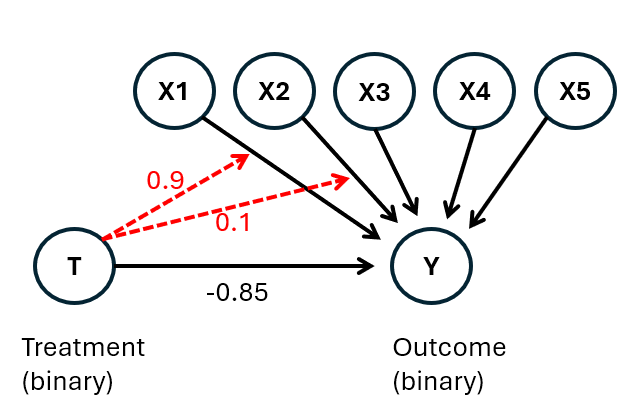
\includegraphics[width=0.3\textwidth]{img/results_ITE_simulation/simulation_observed.png}
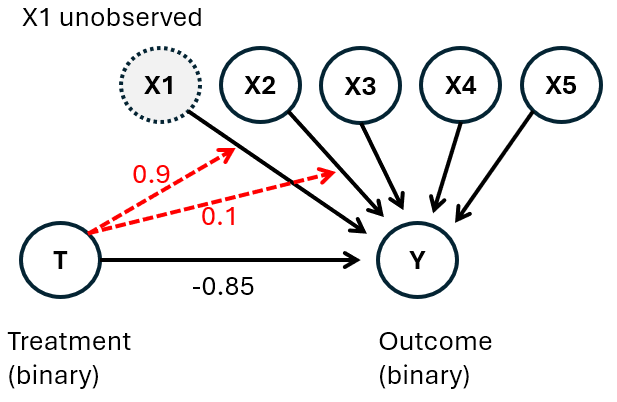
\includegraphics[width=0.3\textwidth]{img/results_ITE_simulation/simulation_unobserved.png}
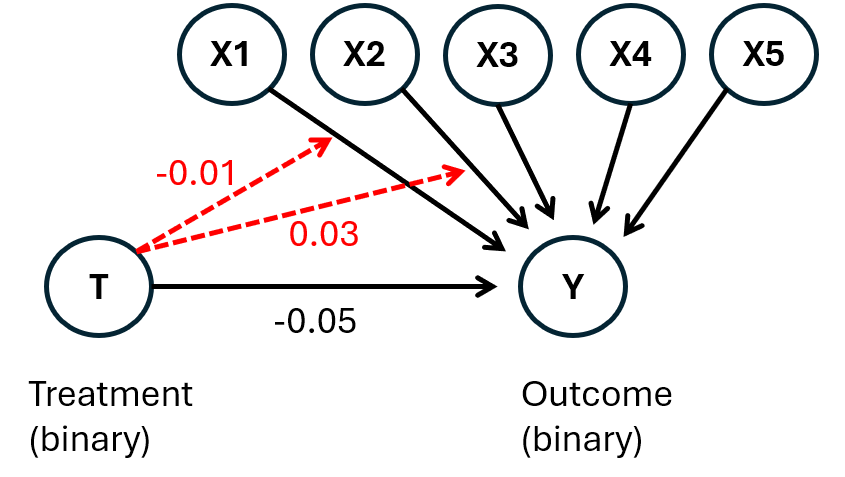
\includegraphics[width=0.3\textwidth]{img/results_ITE_simulation/simulation_small_effects.png}
\caption{Data-generating process (DGP) for the three scenarios in the ITE simulation study (RCT). Interaction effects between treatment ($T$) and covariates ($X_1$ and $X_2$) on the outcome ($Y$) are shown in red. Left: Scenario 3.1, where all covariates are observed and both treatment effect and heterogeneity are strong; Middle: Scenario 3.2, with the same DGP as in Scenario 3.1, but where covariate $X_1$ is not observed; Right: Scenario 3.3, where the treatment effect and heterogeneity are weak, and all covariates are observed.}
\label{fig:simulation_dags}
\end{figure}




% The data is generated for three different scenarios, where the coefficients are set to different values to represent different treatment effects and interaction effects and by removing the covariate $X1$ from the final dataset in scenario 2, hence making it unobserved. The scenarios are summarized in Table \ref{tab:simulation_scenarios}.


% Table with szenarios:

% Szenario 1: 
% description: strong direct and interaction effect of treatment, fully observed
% coefficients: \beta_0 = 0.45, \beta_T = -0.85,  \boldsymbol{\beta}_X = c(-0.5, 0.8, 0.2, 0.6, -0.4), \boldsymbol{\beta}_{TX} = c(0.9, 0.1)
% motivation: this scenario should represent the ideal case where there is high heterogeneity and all variables are observed, hence the ITE estimation is assumed to work well.

% Szenario 2:
% description: strong direct and interaction effect of treatment, but covariate X1 not observed
% coefficients: \beta_0 = 0.45, \beta_T = -0.85,  \boldsymbol{\beta}_X = c(-0.5, 0.8, 0.2, 0.6, -0.4), \boldsymbol{\beta}_{TX} = c(0.9, 0.1)
% motivation: removing the covariate X1, which is responsible for much of the heterogeneity, should cause difficulties in ITE estimation because the heterogeneity can not be attributed to the right covariate.

% Szenario 3:
% description: weak direct and interaction effect of treatment, fully observed
% coefficients: \beta_0 = 0.45, \beta_T = -0.05,  \boldsymbol{\beta}_X = c(-0.5, 0.8, 0.2, 0.6, -0.4), \boldsymbol{\beta}_{TX} = c(-0.01, 0.03)
% motivation: this scenario should represent the case where the treatment effect is weak and heterogeneity is low, hence the model should estimate only small range of ITE.





% \subsubsection*{Scenario 1: Strong effects, all covariates observed}
% 
% This scenario represents an ideal case in which the treatment has a strong direct and interaction effect. All covariates are observed, supposedly enabling effective ITE estimation. The coefficients are set as follows:
% 
% 
% 
% % X1 and X2 interact with treatment
% \begin{align*}
%     \beta_0 &= 0.45,\quad \beta_T = -0.85, \\
%     \boldsymbol{\beta}_X &= (-0.5,\ 0.8,\ 0.2,\ 0.6,\ -0.4), \\
%     \boldsymbol{\beta}_{TX} &= (0.9,\ 0.1) , X_1 \text{ and } X_2 \text{ interact with treatment}
% \end{align*}
% 
% \vspace{0.5em}
% 
% \subsubsection*{Scenario 2: Strong effects, covariate \boldmath$X_1$ unobserved}
% 
% This scenario uses the same coefficients as Scenario 1, but with covariate $X_1$ removed from the dataset. As $X_1$ drives a large portion of the treatment effect heterogeneity, the estimation of the ITE is expected to be biased or incomplete when $X_1$ is not observed.
% 
% 
% \begin{align*}
%     \beta_0 &= 0.45,\quad \beta_T = -0.85, \\
%     \boldsymbol{\beta}_X &= (-0.5,\ 0.8,\ 0.2,\ 0.6,\ -0.4), \\
%     \boldsymbol{\beta}_{TX} &= (0.9,\ 0.1) , X_1 \text{ and } X_2 \text{ interact with treatment}
% \end{align*}
% \textit{Note: $X_1$ is not included in the final dataset.}
% 
% \vspace{0.5em}
% 
% \subsubsection*{Scenario 3: Weak Effects, All Covariates Observed}
% 
% This scenario illustrates a setting with minimal treatment effect and weak treatment-covariate interaction. While all covariates are observed, the model is expected to recover only low-variance ITEs due to limited signal.
% 
% \begin{align*}
%     \beta_0 &= 0.45,\quad \beta_T = -0.05, \\
%     \boldsymbol{\beta}_X &= (-0.5,\ 0.8,\ 0.2,\ 0.6,\ -0.4), \\
%     \boldsymbol{\beta}_{TX} &= (-0.01,\ 0.03), X_1 \text{ and } X_2 \text{ (weakly) interact with treatment}
% \end{align*}


\textbf{Models for ITE estimation:} We applied the following models in \texttt{R} to estimate individualized treatment effects (ITEs) according to Equation~\ref{eq:ITE_binary}: T-learner logistic regression (\texttt{stats} package), T-learner and S-learner logistic lasso regression (\texttt{glmnet} package \citep{friedman2010}, with $\lambda$ selected via 10-fold cross-validation), T-learner random forest (\texttt{randomForest} package \citep{breiman2001}, 100 trees), and T-learner tuned random forest (\texttt{comets} package \citep{comets}, which tunes \texttt{mtry} and \texttt{max.depth} using out-of-bag error, 500 trees).

While all models were run, we focus on two for the main results: the T-learner logistic regression as a baseline (matching the DGP), and the T-learner tuned random forest as a more flexible non-parametric model. Results for the default random forest in Scenario 3.1 are shown in Appendix~\ref{sec:default_rf_ite} to highlight the role of model tuning in avoiding overfitting and ensuring proper calibration.

Each model was trained and evaluated on independent datasets of 10,000 samples generated from the same DGP. Although TRAM-DAGs are well suited for ITE estimation, we did not include them here, as the goal of this experiment is to compare simpler and more complex models under varying conditions. Furthermore, when specified as T-learner with standard logistic latent distribution and linear shift effects of covariates, the TRAM-DAG would be equivalent to a logistic regression for the binary outcome.
% 
% 
% \textbf{Models for ITE estimation:} We applied the following models in \texttt{R} to estimate the ITEs: T-learner logistic regression (\texttt{stats} package), T-learner logistic lasso regression (\texttt{glmnet} package \citep{friedman2010}, with the regularization parameter $\lambda$ estimated via 10-fold cross-validation), S-learner logistic lasso regression (same as the T-learner), T-learner random forest (\texttt{randomForest} package \citep{breiman2001}, 100 trees), and T-learner tuned random forest (\texttt{comets} package \citep{comets}, which tunes the number of variables considered for splitting at each node (\texttt{mtry}) and the maximum tree depth (\texttt{max.depth}) using out-of-bag error, 500 trees). 
% 
% While all models were applied, we present only the results of the T-learner logistic regression as a benchmark (same model as used in the data-generating process), and the tuned random forest as representation of a complex non-parametric model. In Appendix~\ref{sec:default_rf_ite}, we additionally present the results for a standard random forest evaluated for Scenario 1 to illustrate the importance of model tuning to prevent overfitting and ensure accurate calibration.
% 
% All models were trained on a training set and evaluated on a test set, each consisting of 10,000 samples generated from the same DGP. TRAM-DAGs would also be well suited for ITE estimation in this setting, but we chose not to apply them in this experiment, since the main objective is to assess behavioral differences between complex and simple models under different scenarios. TRAM-DAGs are applied in other experiments in this thesis.

\medskip

\textbf{Model evaluation:} Model performance is evaluated visually on both the training and test datasets. For predictive performance, we present true vs. predicted probabilities $P(Y = 1 \mid X, T)$ to assess how well each model is calibrated. Plots of true vs. predicted ITEs (calculated according to Equation~\ref{eq:ITE_binary}) show how closely the model estimates match the true effects. Since the true probabilities and ITEs are known by design in this simulation, direct evaluation of calibration and prediction accuracy is possible, unlike in real-world applications.

To assess whether estimated ITEs correspond to actual observed outcomes, we use ITE-ATE plots. These show the observed average treatment effect (ATE), calculated as $P(Y = 1 \mid T = 1) - P(Y = 1 \mid T = 0)$, in the respective subgroups of estimated ITEs. Accurate models should produce ITE-ATE points that align with the identity line.

These simulation scenarios allow us to assess ITE estimation performance under challenging conditions such as omitted variables and weak treatment effects. The subsequent results reveal which models remain robust under such violations and provide insight into possible real-world estimation failures.




\subsection{Results and discussion} \label{sec:results_experiment3}

In this section, we present the performance of two causal machine learning models -- T-learner logistic regression and T-learner tuned random forest -- for estimating ITEs under the three simulated scenarios introduced in Section~\ref{sec:methods_experiment3}. Scenario~3.1 (Section~\ref{sec:exp3_sc1}) represents the ideal case where all covariates are observed and both treatment and interaction effects are strong. In Scenario~3.2 (Section~\ref{sec:exp3_sc3}), a key effect modifier is unobserved, and in Scenario~3.3 (Section~\ref{sec:exp3_sc3}), treatment and interaction effects are weak, but all covariates are observed.

% Results for all scenarios are presented in Figures~\ref{fig:fully_observed_glm_tlearner} to~\ref{fig:small_interaction_tuned_rf_tlearner}.



\subsubsection{Scenario 3.1: Fully observed, large effects} \label{sec:exp3_sc1}







\begin{figure}[htbp]
\centering
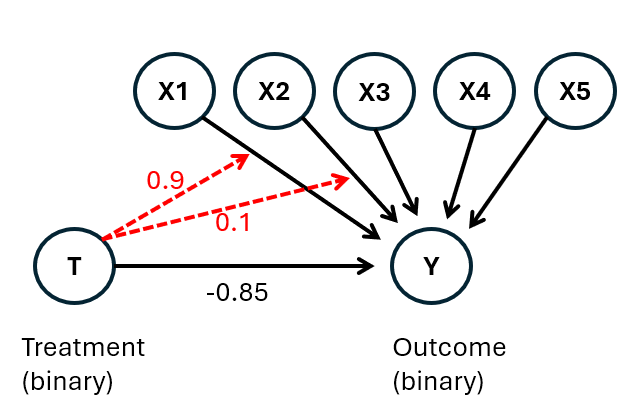
\includegraphics[width=0.35\textwidth]{img/results_ITE_simulation/simulation_observed.png}
\caption{DAG for Scenario~3.1, where all variables are observed and both treatment and interaction effects are strong. This DAG was previously shown in Figure~\ref{fig:simulation_dags} and is re-plotted here for convenience. The numbers indicate the coefficients on the log-odds scale. Red arrows represent interaction effects between treatment ($T$) and covariates ($X_1$ and $X_2$) on the outcome ($Y$).}
\label{fig:fully_observed_dag}
\end{figure}


In Scenario~3.1 (Figure~\ref{fig:fully_observed_dag}),  where treatment effect heterogeneity was large and all covariates were observed, the T-learner logistic regression accurately estimated the ITE. The observed ATE, conditional on the respective ITE subgroup, was well calibrated in both the training and test datasets (Figure~\ref{fig:fully_observed_glm_tlearner}). This is as expected, since the data were generated with the same model class (logistic regression), and applying logistic regression as a T-learner for ITE estimation can accurately capture the interaction effects.

\begin{figure}[htbp]
\centering
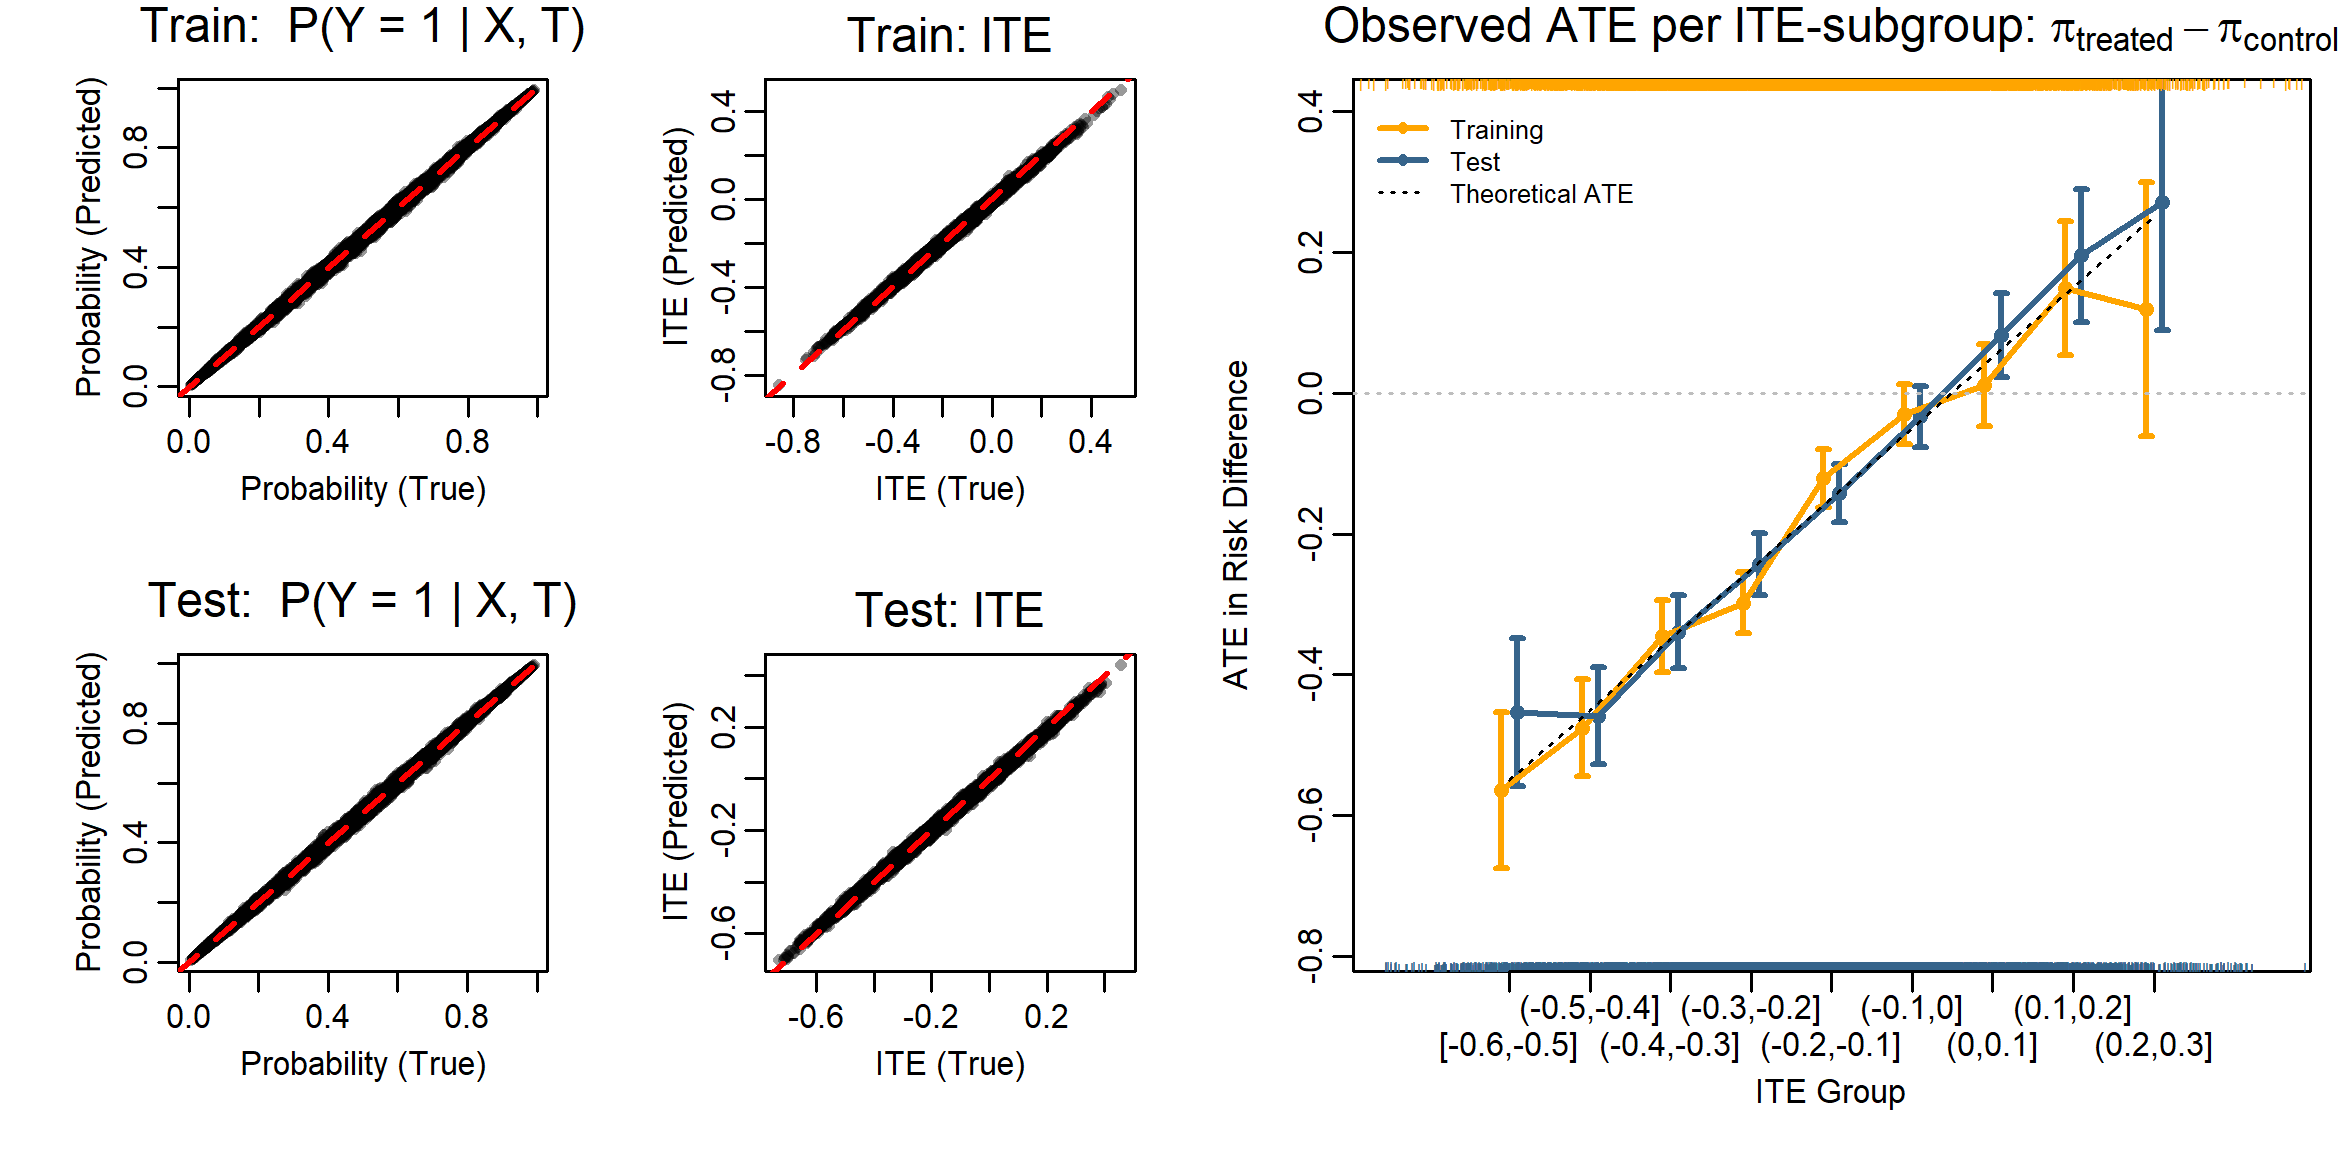
\includegraphics[width=0.9\textwidth]{img/results_ITE_simulation/fully_observed_glm_tlearner.png}
\caption{Results of the T-learner logistic regression in Scenario~3.1, where the DAG is fully observed and both treatment and interaction effects are strong. Left: true vs. predicted probabilities for $P(Y = 1 \mid X, T)$; Middle: true vs. predicted ITEs; Right: observed ATE in terms of risk difference per estimated ITE subgroup.}
\label{fig:fully_observed_glm_tlearner}
\end{figure}



The tuned random forest model also performed well (see Figure~\ref{fig:fully_tuned_rf_tlearner}), but less accurate compared to the logistic model (see Figure~\ref{fig:fully_observed_glm_tlearner}). Choosing a different model class than that used in the DGP may lead to worse prediction accuracy in terms of $P(Y = 1 \mid X, T)$ and ITE. This difference between the two models arises because the logistic regression model has only a small number of parameters, and with sufficient data, these parameters can converge to their true values as used in the logistic DGP, allowing near-perfect recovery of the true probabilities and thus ITEs. In contrast, the non-parametric random forest must infer the underlying probabilities from the observed binary outcomes (0 or 1), which are themselves realizations of a Bernoulli process. This introduces inherent noise, making it harder for the model to estimate the true risk accurately -- even with large sample sizes. Nonetheless, the tuned random forest also captured the general trend of the ITEs, as reflected in the ITE-ATE plot, Figure~\ref{fig:fully_tuned_rf_tlearner}. Both models were able to capture treatment effect heterogeneity well under full observability of covariates.





\begin{figure}[htbp]
\centering
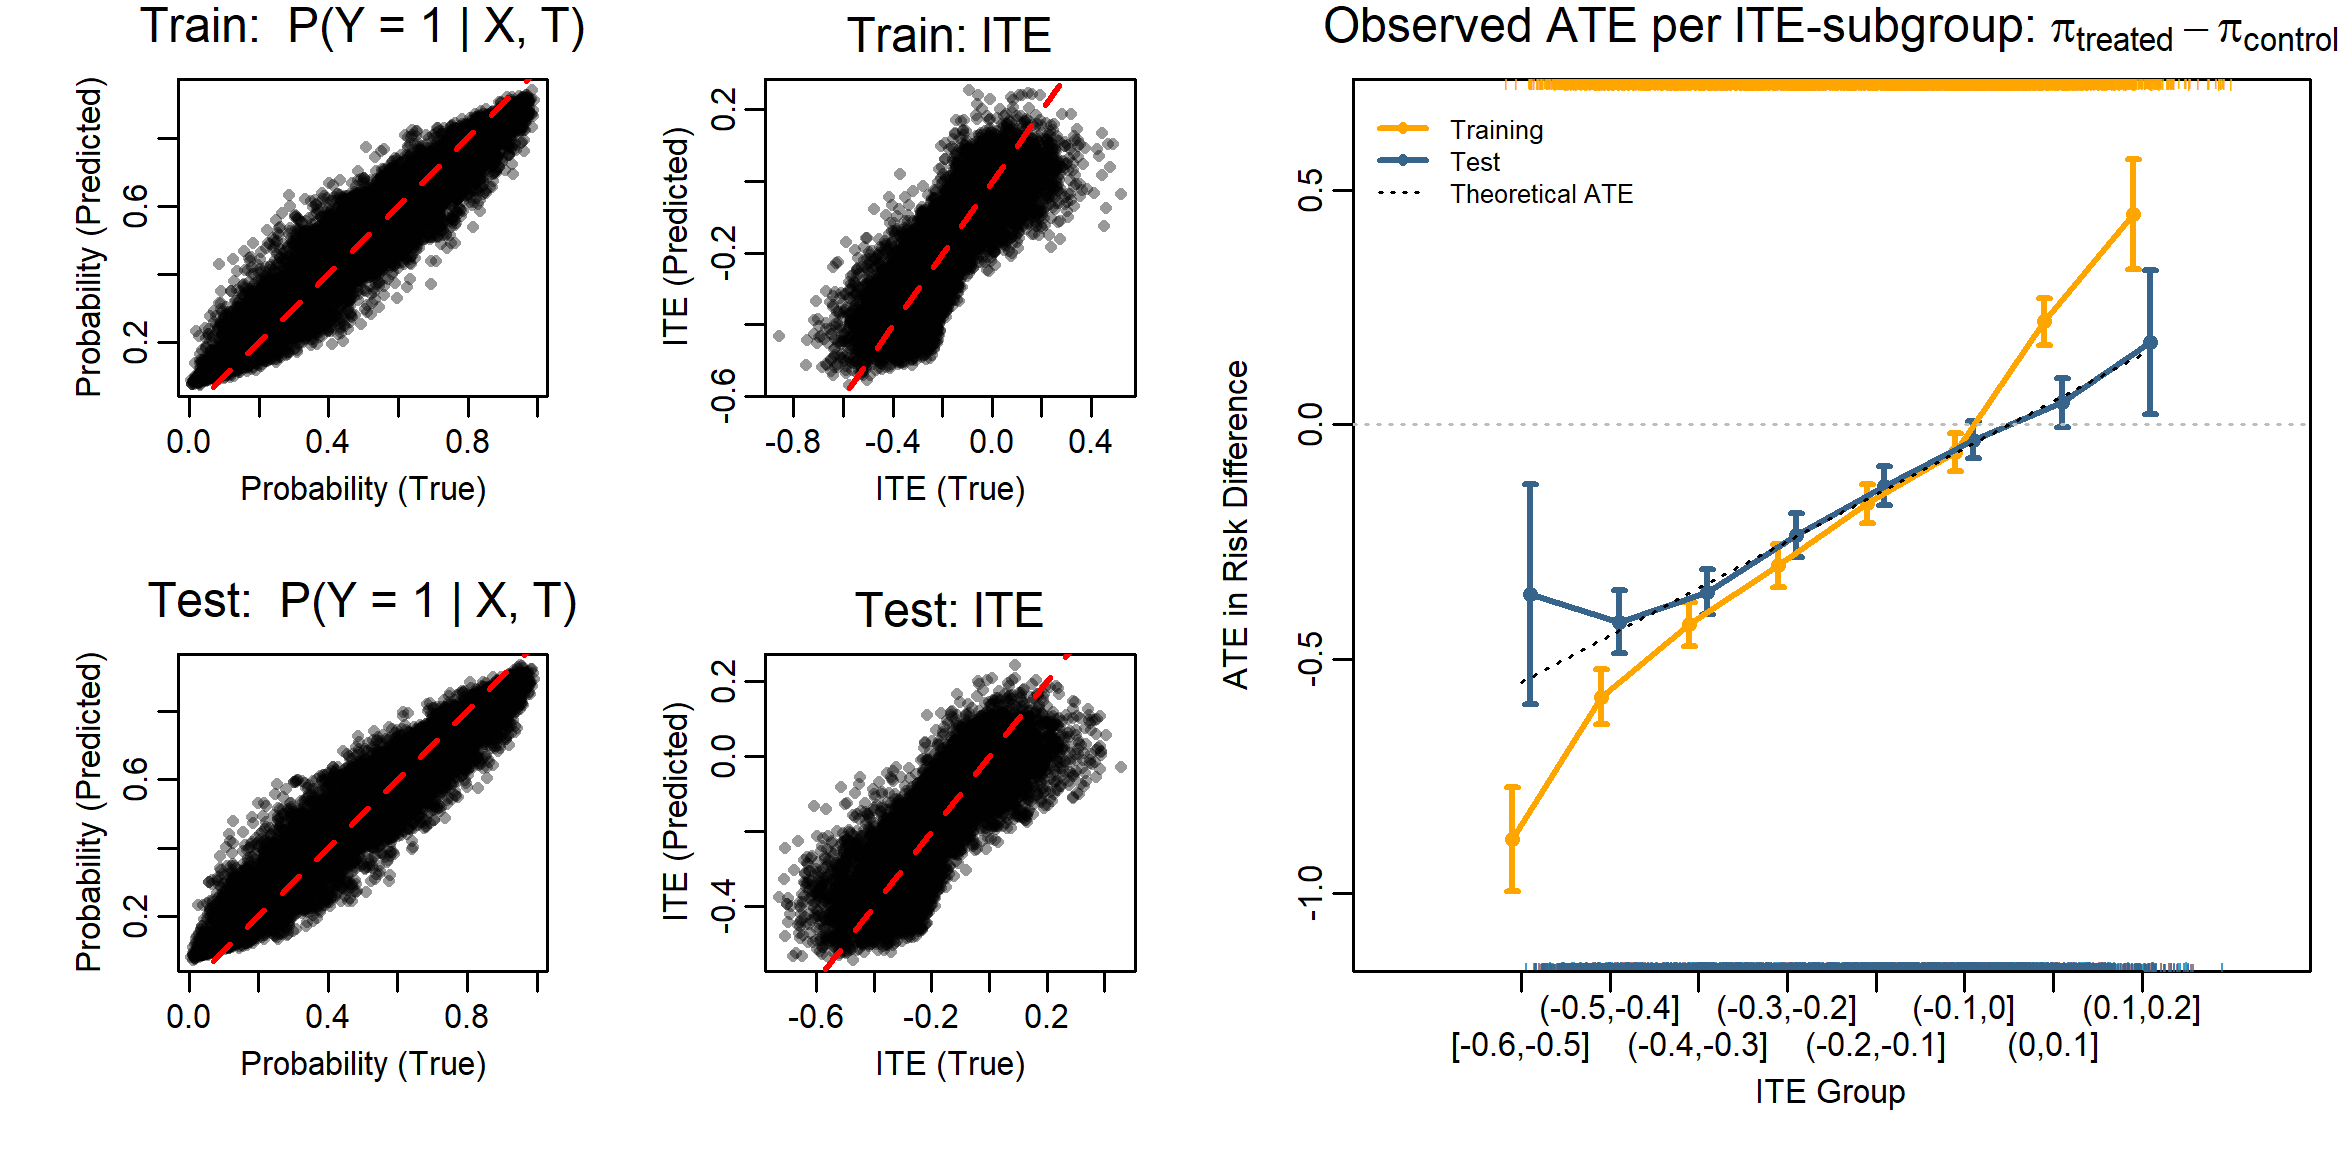
\includegraphics[width=0.9\textwidth]{img/results_ITE_simulation/fully_observed_tuned_rf_tlearner.png}
\caption{Results of the T-learner tuned random forest in Scenario~3.1, where the DAG is fully observed and both treatment and interaction effects are strong. Left: true vs. predicted probabilities for $P(Y = 1 \mid X, T)$; Middle: true vs. predicted ITEs; Right: observed ATE in terms of risk difference per estimated ITE subgroup.}
\label{fig:fully_tuned_rf_tlearner}
\end{figure}


In contrast, the default random forest (i.e., without hyperparameter tuning) performed worse than its tuned counterpart (see Appendix~\ref{sec:default_rf_ite}). As shown in the corresponding ITE-ATE plot, Figure~\ref{fig:fully_observed_rf}, the model exhibited poor calibration and inaccurate ITE estimates, highlighting the importance of proper tuning to ensure reliable ITE estimation and avoid overfitting.


\clearpage



\subsubsection{Scenario 3.2: Unobserved interaction} \label{sec:exp3_sc2}

\begin{figure}[htbp]
\centering
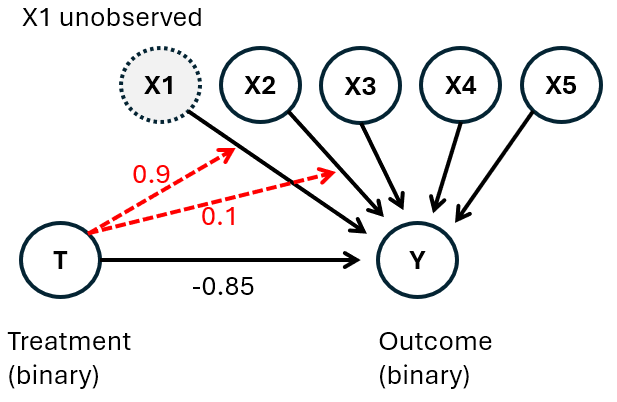
\includegraphics[width=0.35\textwidth]{img/results_ITE_simulation/simulation_unobserved.png}
\caption{DAG for Scenario~3.2, where there are strong treatment and interaction effects, but variable $X_1$ is not observed. This DAG was previously shown in Figure~\ref{fig:simulation_dags} and is re-plotted here for convenience. The numbers indicate the coefficients on the log-odds scale. Red arrows represent interaction effects between treatment ($T$) and covariates ($X_1$ and $X_2$) on the outcome ($Y$).}
\label{fig:unobserved_interaction_dag}
\end{figure}


In Scenario~3.2 (Figure~\ref{fig:unobserved_interaction_dag}), where treatment effect heterogeneity remained large but one important interaction covariate ($X_1$) was not observed, prediction accuracy decreased for both models, and the estimated heterogeneity in terms of the ITE was smaller than the true heterogeneity (see true vs. estimated ITE plots in Figures~\ref{fig:unobserved_interaction_glm_tlearner} and~\ref{fig:unobserved_interaction_tuned_rf_tlearner}). 

Although a considerable number of individuals had a true ITE that was positive (visible in the true vs. estimated ITE plot in Figure~\ref{fig:unobserved_interaction_glm_tlearner}), the T-learner logistic regression did not predict a single positive ITE. This shows that the missing covariate $X_1$ in this example prevents detection of individuals who would actually benefit from the treatment. In practice, where the true ITEs are unknown, we would evaluate the ITE estimation in terms of the ITE-ATE plot (Figure~\ref{fig:unobserved_interaction_glm_tlearner}), which in this case would suggest good calibration of ITEs, as they follow the identity-line. However, we still did not identify the patients that would actually benefit from the treatment. This implies that even if the ITE-ATE plot suggests heterogeneity and that ITE estimates are well calibrated, there may still be additional heterogeneity, which was not captured by the model.






\begin{figure}[htbp]
\centering
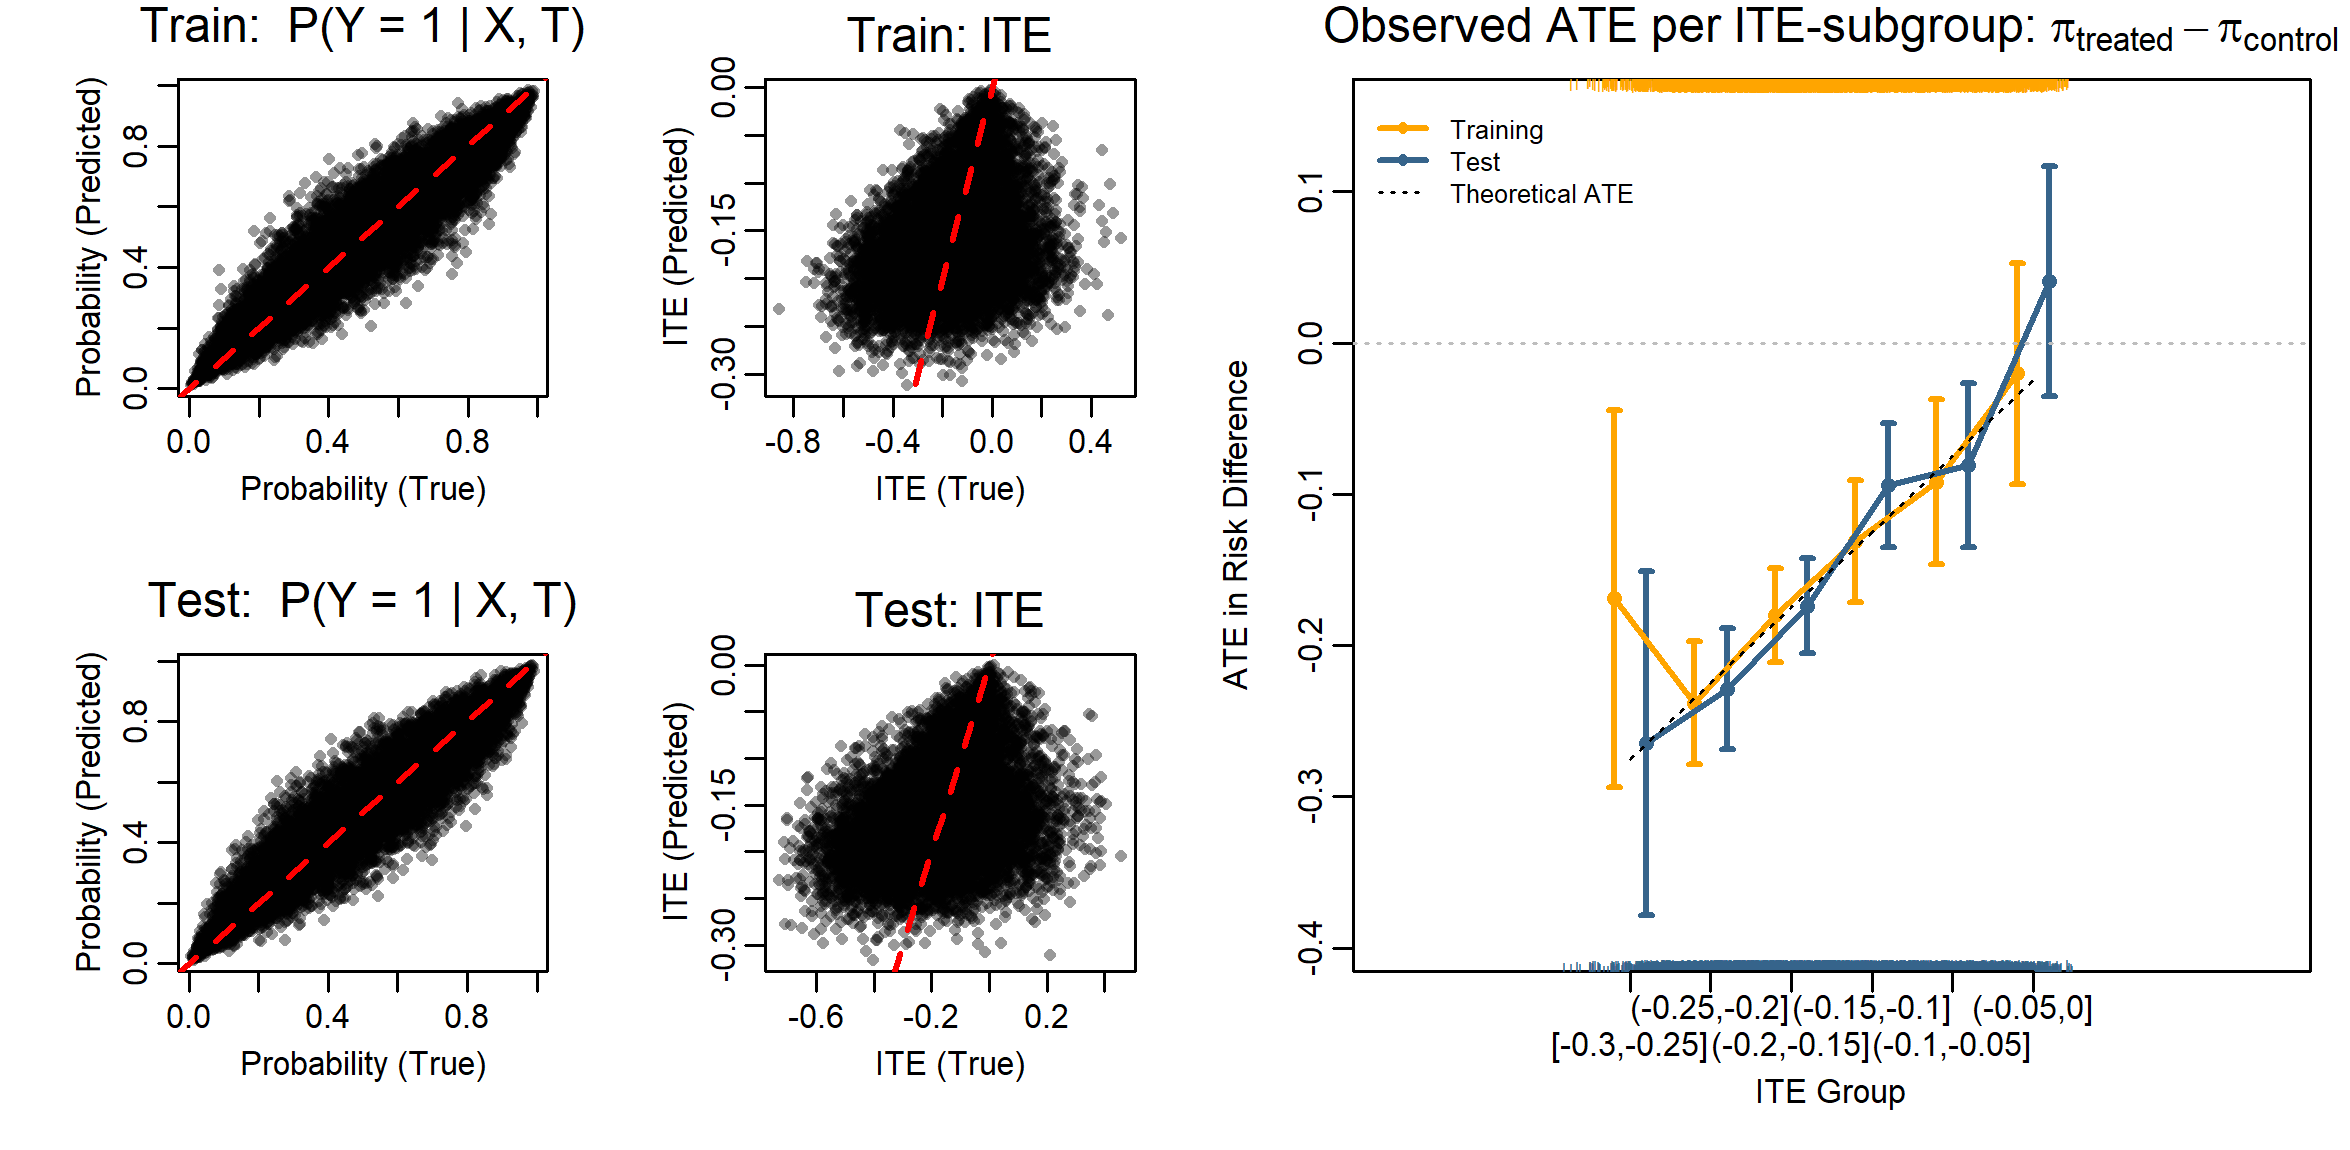
\includegraphics[width=0.9\textwidth]{img/results_ITE_simulation/unobserved_interaction_glm_tlearner.png}
\caption{Results of the T-learner logistic regression in Scenario~3.2, where there are strong treatment and interaction effects, but variable $X_1$ is not observed. Left: true vs. predicted probabilities for $P(Y = 1 \mid X, T)$; Middle: true vs. predicted ITEs; Right: observed ATE in terms of risk difference per estimated ITE subgroup.}
\label{fig:unobserved_interaction_glm_tlearner}
\end{figure}


In contrast, the T-learner tuned random forest (Figure~\ref{fig:unobserved_interaction_tuned_rf_tlearner}) estimated larger treatment effect heterogeneity than the logistic model, but still could not accurately estimate the ITE and also failed to detect patients who would benefit from the treatment. The ITE-ATE plot in Figure~\ref{fig:unobserved_interaction_tuned_rf_tlearner} illustrates that the model discriminates too strongly in the training set and does not generalize well to the test set.



\begin{figure}[htbp]
\centering
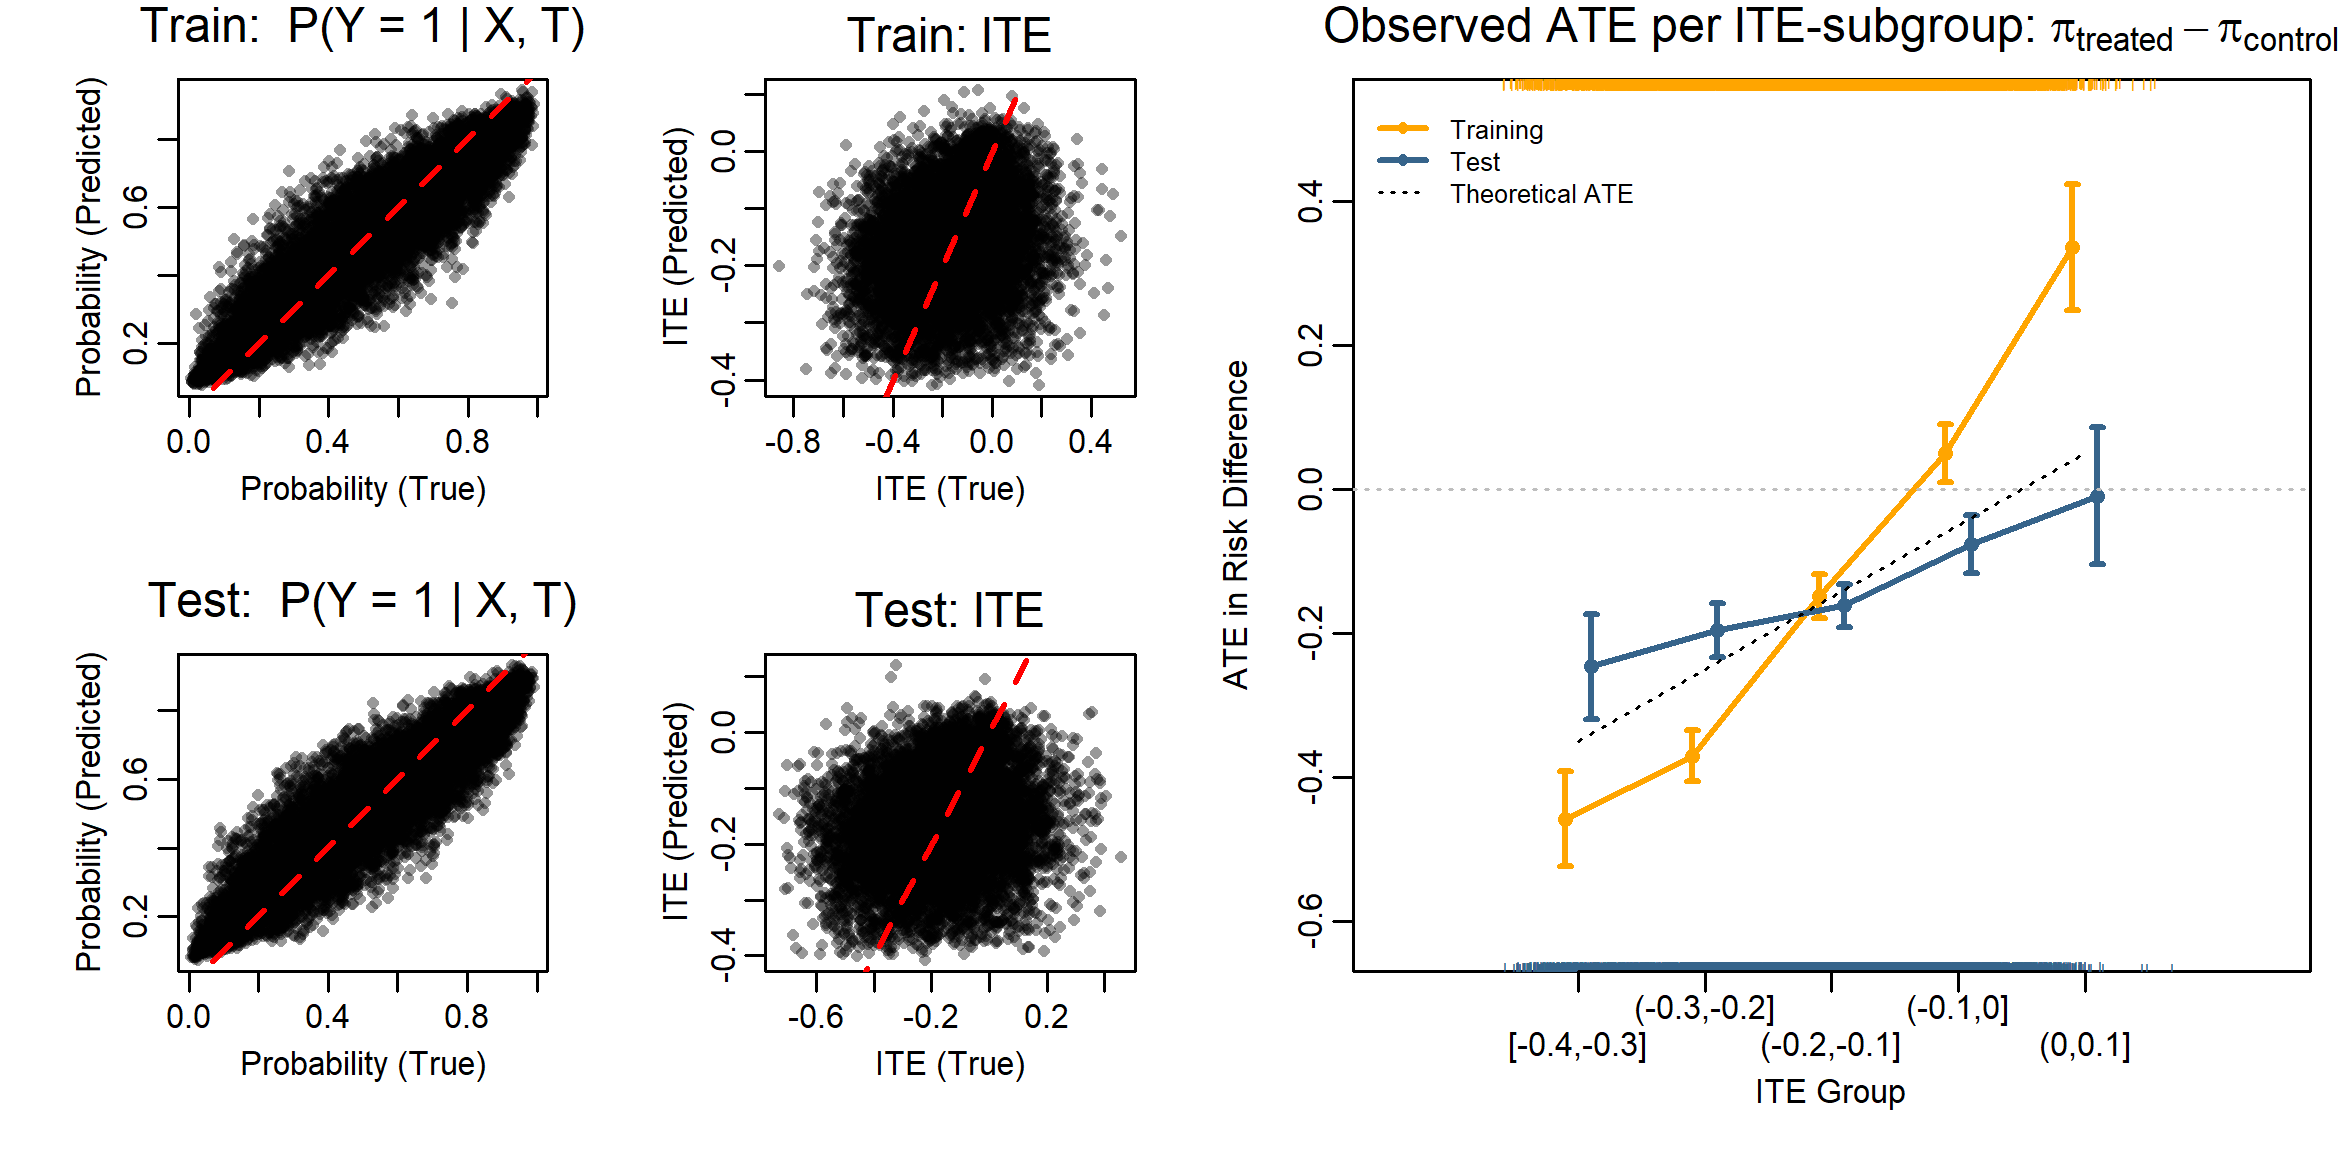
\includegraphics[width=0.9\textwidth]{img/results_ITE_simulation/unobserved_interaction_tuned_rf_tlearner.png}
\caption{Results of the T-learner tuned random forest in Scenario~3.2, where there are strong treatment and interaction effects, but variable $X_1$ is not observed. Left: true vs. predicted probabilities for $P(Y = 1 \mid X, T)$; Middle: true vs. predicted ITEs; Right: observed ATE in terms of risk difference per estimated ITE subgroup.}
\label{fig:unobserved_interaction_tuned_rf_tlearner}
\end{figure}


\clearpage

\subsubsection{Scenario 3.3: Fully observed, small effects} \label{sec:exp3_sc3}

\begin{figure}[htbp]
\centering
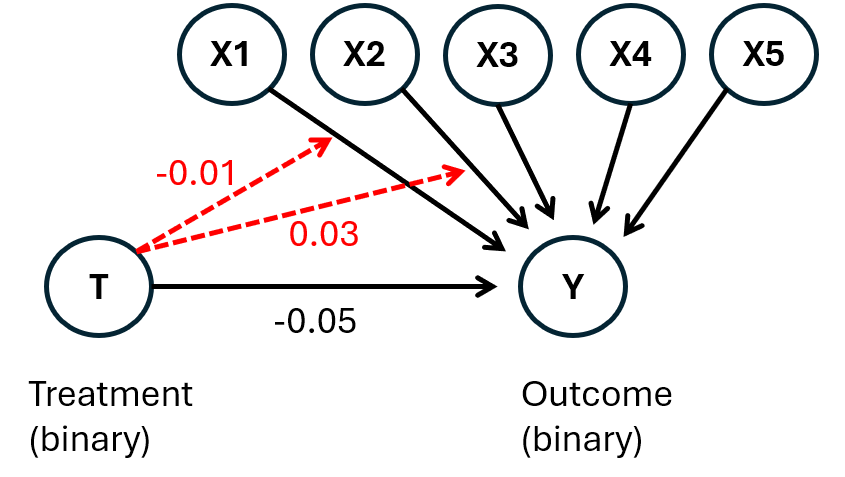
\includegraphics[width=0.35\textwidth]{img/results_ITE_simulation/simulation_small_effects.png}
\caption{DAG for Scenario~3.3, where all variables are observed and both treatment and interaction effects are weak. This DAG was previously shown in Figure~\ref{fig:simulation_dags} and is re-plotted here for convenience. The numbers indicate the coefficients on the log-odds scale. Red arrows represent interaction effects between treatment ($T$) and covariates ($X_1$ and $X_2$) on the outcome ($Y$).}
\label{fig:small_interaction_dag}
\end{figure}




In Scenario~3.3 (Figure~\ref{fig:small_interaction_dag}), where the true treatment effect heterogeneity was small and all covariates were observed, the T-learner logistic regression estimated a larger heterogeneity than actually present (see true vs. estimated ITE plots in Figure~\ref{fig:small_interaction_glm_tlearner}). In the ITE-ATE plot in Figure~\ref{fig:small_interaction_glm_tlearner}, the confidence intervals of all ITE subgroups overlap and include the zero line, indicating that the treatment effect is not significantly different from zero. This matches expectations given the small true effect sizes.



\begin{figure}[htbp]
\centering
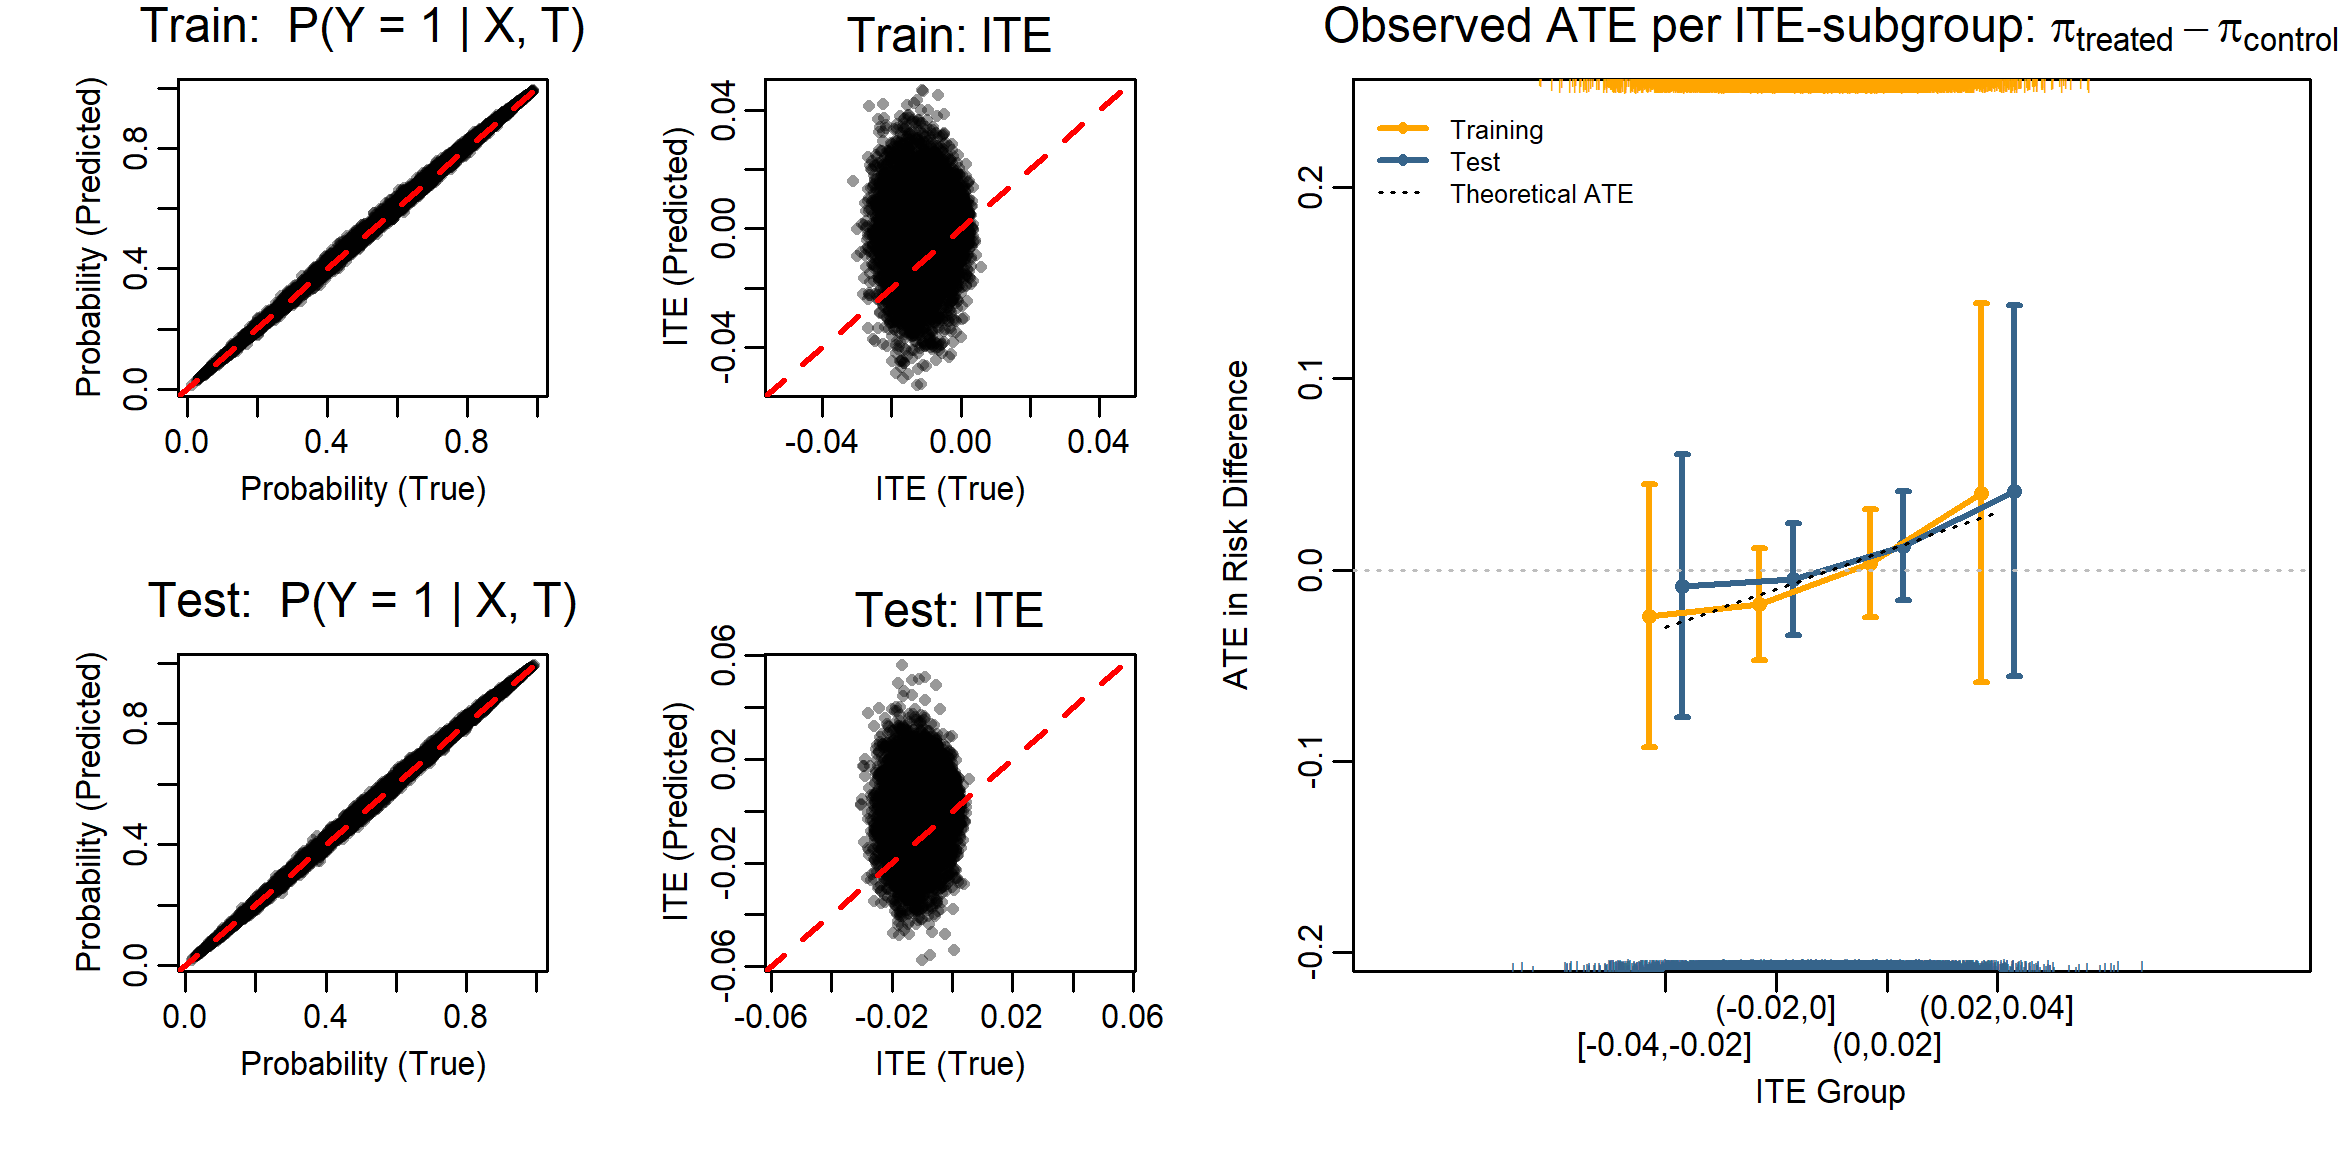
\includegraphics[width=0.9\textwidth]{img/results_ITE_simulation/small_interaction_glm_tlearner.png}
\caption{Results of the T-learner logistic regression in Scenario~3.3, where the DAG is fully observed and both treatment and interaction effects are weak. Left: true vs. predicted probabilities for $P(Y = 1 \mid X, T)$; Middle: true vs. predicted ITEs; Right: observed ATE in terms of risk difference per estimated ITE subgroup.}
\label{fig:small_interaction_glm_tlearner}
\end{figure}


However, the T-learner tuned random forest model incorrectly estimated even larger treatment effect heterogeneity than the logistic regression model (see true vs. estimated ITE plots in Figure~\ref{fig:small_interaction_tuned_rf_tlearner}). As shown in the ITE-ATE plot in Figure~\ref{fig:small_interaction_tuned_rf_tlearner}, the model exhibited strong discrimination in the training set but did not replicate this pattern in the test set, where -- regardless of the estimated ITE -- the observed outcomes were similar across all subgroups. These results indicate that when evaluating the ITE predictions on the test set, it correctly suggests that no significant treatment effect heterogeneity is present.



\begin{figure}[htbp]
\centering
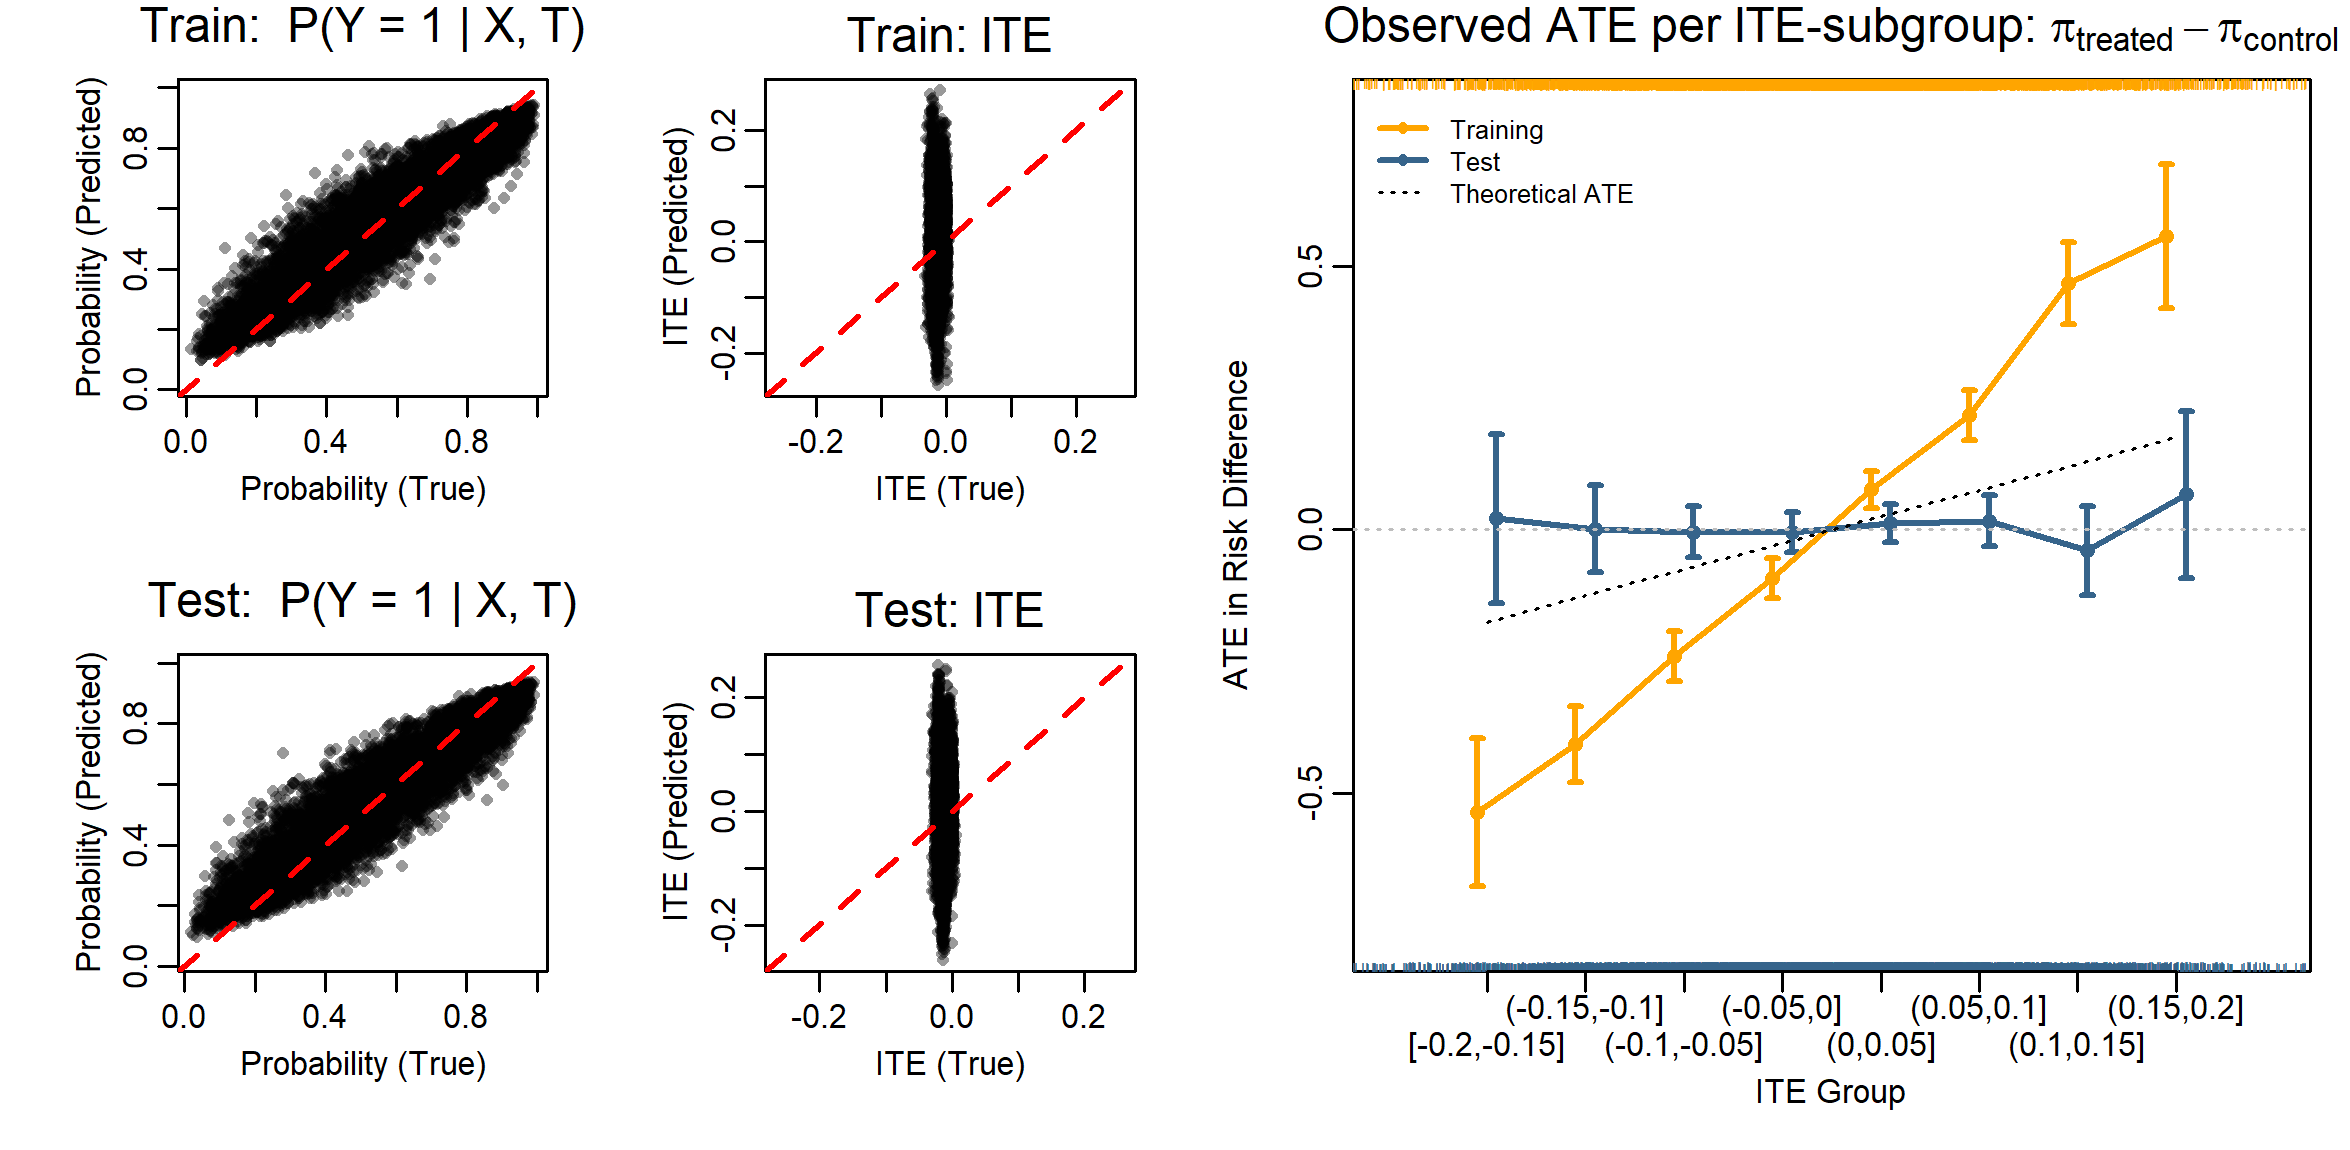
\includegraphics[width=0.9\textwidth]{img/results_ITE_simulation/small_interaction_tuned_rf_tlearner.png}
\caption{Results of the T-learner tuned random forest in Scenario~3.3, where the DAG is fully observed and both treatment and interaction effects are weak. Left: true vs. predicted probabilities for $P(Y = 1 \mid X, T)$; Middle: true vs. predicted ITEs; Right: observed ATE in terms of risk difference per estimated ITE subgroup.}
\label{fig:small_interaction_tuned_rf_tlearner}
\end{figure}


% enforce that starts after all floats have been displayed
\FloatBarrier




\subsection{Discussion of Experiment 3} \label{sec:disc_experiment3}



Tuning more flexible models like random forests using cross-validation improved generalization to the test set but led to poor calibration in terms of predicted probabilities vs. empirically observed outcomes in the training set. An illustrative case is shown in Appendix~\ref{sec:calibration_tuned_rf} for the T-learner tuned random forest in Scenario~3 (with weak effects; Section~\ref{sec:exp3_sc3}), where calibration was poor in the training set but aligned well with the identity line in the test set. We repeatedly observed this pattern in the tuned random forest when, in the ITE-ATE plot, results from the training set did not generalize to the test set (e.g. in Figures~\ref{fig:unobserved_interaction_tuned_rf_tlearner} and~\ref{fig:small_interaction_tuned_rf_tlearner}). This highlights the importance of evaluating models on an independent test set, when tuning a model to prevent overfitting, although evaluation on a test set should be done in any case.

\medskip

In this experiment, we showed that even when causal ML models for ITE estimation are well calibrated in terms of prediction accuracy $P(Y = 1 \mid \mathbf{X}, T)$, they can still fail to estimate the ITE accurately under less favorable scenarios. In cases of full observability of covariates but low interaction effects (Scenario~3.3; Section~\ref{sec:exp3_sc3}), models may estimate too high heterogeneity that is not present in the data. However, this can become visible in the ITE-ATE plot on the test set, which reveals that the apparent heterogeneity does not generalize. 
But we also observed that when important effect-modifying covariates are missing (Scenario~3.2; Section~\ref{sec:exp3_sc2}), the models may fail to detect treatment effect heterogeneity altogether. In such cases, the estimated ITEs may be too small or even negative, suggesting that the model does not capture the true treatment effect heterogeneity. This makes it difficult to distinguish between a true lack of heterogeneity and the failure to capture it due to unobserved effect modifiers.


\citet{vegetabile2021} also analyzed the effect of unobserved interaction variables. He pointed out that as long as all confounding variables $\mathbf{X}$ are observed and conditioned on, the ignorability assumption (Equation~\ref{eq:ignorability}) required for ITE estimation is satisfied -- even in the presence of an unobserved interaction variable $Z$. However, if such a variable $Z$ exists, the estimated ITEs would be biased, and this issue could arise even in an RCT setting where confounding is removed through randomization. This aligns with our observations in Scenario~3.2 (Section~\ref{sec:exp3_sc2}).

\citet{nichols2007} discusses various methods for estimating causal effects from observational data, including in the presence of unobserved variables. One of these methods, instrumental variables (IV), can help reduce bias from unobserved confounding. Whether IV methods can also address unobserved effect modifiers in the context of ITE estimation is not something we explored, and remains beyond the scope of this thesis.



% such as the use of instrumental variables (IV) to estimate CATE in the presence of unobserved confounders \citep{nichols2007, hartford2017}. \citet{frauen2023} propose a model based on IV that is said to also be applicable on observational data. However, this is not yet widely adopted and remains an area for future research.

 % check more details, they also have an example DAG, however it is not yet accepted and still under review










% LaTeX file for Chapter Exp4
















\section{Experiment 4: ITE estimation with TRAM-DAGs (simulation)} \label{ch:exp4}




% quantile treatment effect
% Papers:

% https://journals.sagepub.com/doi/pdf/10.1177/1536867X1001000309
% https://epge.fgv.br/files/1125.pdf



% \subsection{Motivation}
% 
% We claim that the TRAM-DAG framework can be effectively used for unbiased ITE estimation on observational data with confounding and mediating variables, provided that the identifiability assumptions are satisfied and the DAG is fully known. Therefore, we apply TRAM-DAGs in both a confounded and a randomized setting, using data simulated according to the DAGs shown in Figure~\ref{fig:ite_dag_observational}. The binary treatment ($X_4$) is the intervention variable, and the goal is to estimate the ITE for the continuous outcome $Y$. To evaluate how the model performs under more or less favorable conditions, we conduct this experiment under three scenarios: Scenario~(4.1) (Section~\ref{sec:exp4_sc1}) including both direct and interaction effects of treatment, Scenario~(4.2) (Section~\ref{sec:exp4_sc2}) including only a direct effect, and Scenario~(4.3) (Section~\ref{sec:exp4_sc3}) including only interaction effects.

\subsection{Motivation}

We claim that the TRAM-DAG framework can be effectively used for unbiased ITE estimation on observational data that includes both confounding and mediating variables -- provided that identifiability assumptions are met and the underlying DAG is fully known. To evaluate this, we apply TRAM-DAGs in both confounded and randomized settings, using data simulated according to the DAGs shown in Figure~\ref{fig:ite_dag_observational}. The binary treatment variable ($X_4$) represents the intervention, and the goal is to estimate the ITE for a continuous outcome $Y$.

To assess model performance under varying conditions, we conduct this experiment across three scenarios:  

\begin{itemize}
    \item \textbf{Scenario 4.1} (Section~\ref{sec:exp4_sc1}): both direct and interaction effects of treatment are present,
    \item \textbf{Scenario 4.2} (Section~\ref{sec:exp4_sc2}): only a direct treatment effect is included,
    \item \textbf{Scenario 4.3} (Section~\ref{sec:exp4_sc3}): only interaction effects are included.
\end{itemize}


\begin{figure}[H]
\centering
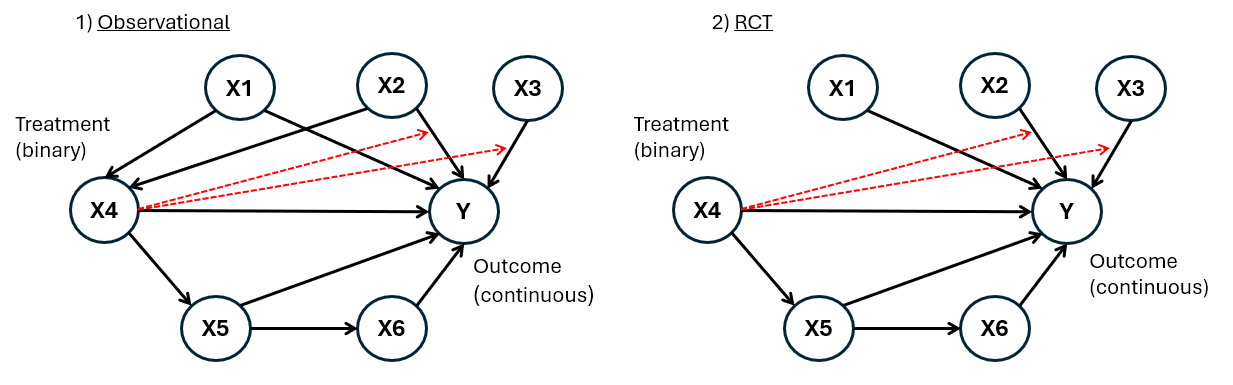
\includegraphics[width=0.85\textwidth]{img/exp4_dags.png}
\caption{DAGs used for the simulation to estimate the ITE. Left: Observational; Right: RCT setting. The source nodes $X_1$, $X_2$, and $X_3$ come from a multivariate standard normal distribution ($\rho=0.1$). In the observational setting, the binary treatment $X_4$ depends on the parents $X_1$ and $X_2$. In the RCT setting, this dependency is omitted due to randomization. The outcome $Y$ depends on all variables, with additional interaction effects between the treatment and the variables $X_2$ and $X_3$. All variables except the treatment $X_4$ are continuous.}
\label{fig:ite_dag_observational}
\end{figure}

\medskip

\textbf{Illustrative scenario:} A possible real-world scenario that follows the structure of the proposed DAG could be the following: A marketing campaign is conducted to increase customer spending. The treatment is the marketing email ($X_4$) sent to customers. If the treatment is not randomized, it depends on prior total spend ($X_1$) and the customer engagement score ($X_2$). The outcome is the total spend in the 30 days following the email, denoted as $Y$. The past total spend ($X_1$) and customer engagement score ($X_2$) act as confounders, influencing both the treatment and the outcome. The customer satisfaction score ($X_3$), obtained from a recent survey, is another predictor. The time spent on the website after receiving the email ($X_5$) is a mediator that affects the number of product pages viewed ($X_6$), which in turn influences the total spend ($Y$). Interaction effects exist between the treatment ($X_4$) and both $X_2$ and $X_3$, meaning the treatment effect differs based on the customer's engagement and satisfaction levels. The goal is to estimate the individualized treatment effect (ITE) of the marketing email ($X_4$) on the total spend ($Y$), in order to personalize customer targeting.

\medskip

\subsection{Setup} \label{sec:methods_experiment4}

\textbf{Data-generating process:} The standard logistic distribution was chosen as the noise distribution to align with other examples in this thesis. Any other noise distribution could also be used here, as we are not interested in coefficient interpretability in this experiment. All variables except the binary treatment $X_4$ are continuous. The source nodes $X_1$, $X_2$, and $X_3$ are generated from a multivariate standard normal distribution with a compound symmetric covariance matrix ($\rho = 0.1$). These variables represent baseline patient characteristics.

In the observational setting, $X_1$ and $X_2$ act as confounders by influencing both the treatment assignment $X_4$ and the outcome $Y$. In the RCT setting, these dependencies are removed due to randomization. The mediator $X_5$ depends on treatment $X_4$, and $X_6$ depends on $X_5$. The log-odds of the continuous outcome $Y$ depend linearly on all covariates, including additional interaction terms between the treatment and $X_2$ and $X_3$. Equation~\ref{eq:outcome_dgp} defines the outcome $Y$ on the log-odds scale:

\begin{equation}
h(y \mid \mathbf{X}) = h_I(y) + \boldsymbol{\beta}_X^\top \mathbf{X} + X_4 \cdot (\boldsymbol{\beta}_{TX}^\top \mathbf{X}_{\text{TX}})
\label{eq:outcome_dgp}
\end{equation}

Here, $h_I(y)$ is the intercept function, $\mathbf{X}$ is the full covariate vector, and $\mathbf{X}_{\text{TX}} = \{X_2, X_3\}$ denotes the interaction covariates that affect the outcome only when treatment is applied ($X_4 = 1$). The intercept function $h_I(y)$ must be smooth and monotonically increasing. We define it as $h_I(y) = \tan(y/2) / 0.2$ for $y \in [-2, 2]$, and extrapolate linearly at the boundaries.

The coefficients are set as $\boldsymbol{\beta}_X = (-0.5,\ 0.5,\ 0.2,\ 1.5,\ -0.6,\ 0.4)$, where the value $1.5$ represents the direct effect of treatment $X_4$ on the outcome. The interaction coefficients are set to $\boldsymbol{\beta}_{TX} = (-0.9,\ 0.7)$.

\medskip

\textbf{Three scenarios:} The experiment is conducted under three different scenarios regarding the effect of the treatment on the outcome $Y$ in the DGP: Scenario 4.1 (Section~\ref{sec:exp4_sc1}) with both direct treatment and interaction effects, Scenario 4.2 (Section~\ref{sec:exp4_sc2}) with only a direct effect, and Scenario 4.3 (Section~\ref{sec:exp4_sc3}) with only interaction effects. Depending on the scenario, the corresponding coefficients in $\boldsymbol{\beta}_X$ and $\boldsymbol{\beta}_{TX}$ in Equation~\ref{eq:outcome_dgp} are set to zero.

\medskip


\textbf{TRAM-DAG estimation:} In both the observational and RCT settings, the TRAM-DAG is fitted as an S-learner (i.e., a single model including the treatment variable). To allow for full flexibility, all nodes with parents are modeled using complex intercepts with three hidden layers of size (10, 10, 10), without applying batch normalization or dropout, using ReLU activation. This architecture enables the model to learn nonlinearities and interactions between the treatment and covariates, allowing it to estimate both potential outcomes. The model is trained on a dataset of 20,000 samples. To prevent overfitting, an additional validation set of 10,000 samples is used, and the final model is selected using early stopping based on the validation loss.

\medskip

\textbf{ITE estimation procedure:} \label{qte:exp4} In contrast to much of the literature we reviewed, where ITEs are typically defined in terms of expected values of potential outcomes (Equation~\ref{eq:ite}), we estimate the quantile treatment effect (QTE), specifically at the median (Equation~\ref{eq:qte}). For each individual, we calculate the difference between the medians of the potential outcome distributions under treatment and control. Note that estimating the potential outcomes in terms of expected values would also be possible -- either by repeatedly sampling from each outcome distribution or, potentially, by numerical integration. However, for this experiment, we chose to estimate the QTE. 
\citet{chernozhukov2005}, for example, highlighted the ability of quantile regression models in heterogeneous treatment effect estimation. QTEs are particularly relevant when the distributional behavior of outcomes beyond the mean is of interest. The median QTE is defined as

\begin{equation}
\text{QTE}^{(0.5)}(\mathbf{x}) = Q_{Y(1) \mid \mathbf{X} = \mathbf{x}}(0.5) - Q_{Y(0) \mid \mathbf{X} = \mathbf{x}}(0.5),
\label{eq:qte}
\end{equation}


where $Q_{Y(t) \mid \mathbf{X} = \mathbf{x}}(q)$ denotes the $q$-th quantile of the potential outcome distribution under treatment $t$.

Once the TRAM-DAG model is fitted on observed data, we can access the inverse transformation functions $X_i = h^{-1}(Z_i \mid \text{pa}(X_i))$, which represent the structural equations of the DAG. ITE estimation proceeds in three steps, according to Algorithm~\ref{alg:ite_qte}. First, the latent values $z_{ij}$ for the explanatory variables $X_i \in \{X_1, X_2, X_3, X_5, X_6\}$ are computed for each sample $j$ using the transformation functions conditioned on their observed parents. Second, the treatment variable $X_4$ is intervened on using the do-operator for both $X_4 = 0$ and $X_4 = 1$. For each of these two treatment states, $X_5$, $X_6$, and the potential outcome (distribution) $Y$ are sampled sequentially using the latent encodings and inverse transformations. This means that the counterfactuals for $X_5$ and $X_6$ are determined. This results in two potential outcome distributions per individual, as illustrated in Figure~\ref{fig:exp4_potential_outcomes}. Finally, for each individual, the median is determined for both potential outcome distributions and the QTE is calculated as the difference between the two medians (Equation~\ref{eq:qte}). 
For simplicity, we will refer to QTEs as ITEs throughout the remainder of the experiment.


\begin{figure}[H]
\centering
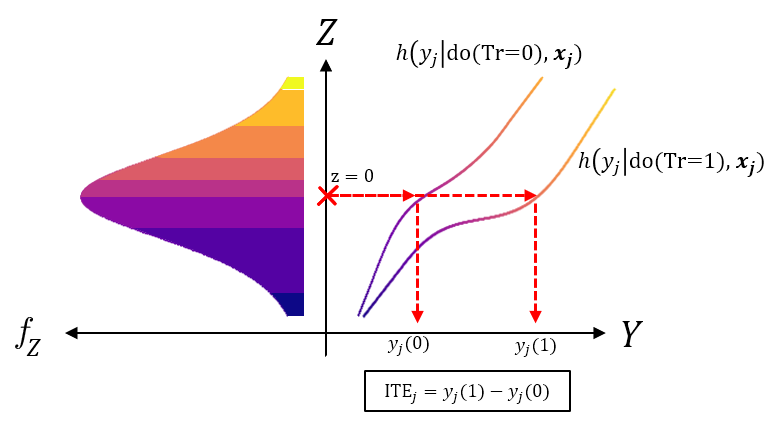
\includegraphics[width=0.6\textwidth]{img/potential_outcomes_y.png}
\caption{ITE estimation in terms of quantile treatment effect (QTE) (Equation~\ref{eq:qte}) at the median with TRAM-DAGs. The two transformation functions represent the distributions of the potential outcomes under both treatments. For the QTE(0.5), the median of the latent distribution (0 for the standard logistic) is evaluated on both transformation functions to determine the median potential outcomes. We define the ITE for an individual as the difference of the median potential outcomes. Plot adapted from visualizations similar to those used in \citet{sick2025}.}
\label{fig:exp4_potential_outcomes}
\end{figure}


\begin{algorithm}
\caption{ITE estimation (QTE) using TRAM-DAGs}
\label{alg:ite_qte}
\begin{algorithmic}
\State \textbf{Input:} Fitted TRAM-DAG, dataset of $n$ individuals
\For{each individual $j = 1$ to $n$}
  \State \textbf{Step 1: Determine latent values}
  \For{each explanatory node $X_i \in \{X_1, X_2, X_3, X_5, X_6\}$}
    \State Compute latent value: $z_{ij} = h_i(x_{ij} \mid \text{pa}(x_{ij}))$
  \EndFor

  \State \textbf{Step 2: Generate potential outcomes under treatment and control}
  \For{$x_4 \in \{0, 1\}$} \Comment{Simulate both treatment states}
    \State Fix $X_4 = x_4$ (intervention)
    \State Sample $X_5$ and $X_6$ sequentially using $z_{ij}$ and inverse transformations
    \State Sample potential outcome $y_j(x_4)$ using $z_{7,j} = 0$ (median of the potential outcome distribution)

  \EndFor

  \State \textbf{Step 3: Compute ITE (QTE) for individual $j$}
  \State $\text{ITE}_j = y_j(1) - y_j(0)$  %\text{median}(y_j(1)) - \text{median}(y_j(0))$
\EndFor
\State \textbf{Output:} ITE estimates $\{\text{ITE}_j\}_{j=1}^n$
\end{algorithmic}
\end{algorithm}


% enforce that starts after all floats have been displayed
\FloatBarrier

\medskip

\textbf{Model evaluation:} Validation is conducted on the training dataset and on an independent test dataset, each of which consists of 20,000 samples. During the data-generating process, the true potential outcomes under both treatment states were recorded for each individual, which allows for exact computation of the true ITE. The estimated ITEs are evaluated against the true values using several visual and numerical metrics. These include density plots of the estimated ITEs (e.g. Figure~\ref{fig:scenario1_ite_densities_train_test}), scatter plots of true vs. estimated ITEs (e.g. Figure~\ref{fig:scenario1_ite_scatter_train_test}), and ITE-ATE plots (e.g. Figure~\ref{fig:observ_scenario1_ite_ATE}) where the observed ATE per ITE subgroup is computed as the difference in medians. In addition, the average of the estimated ITEs is compared to the true average ITE and to the empirical ATE from the RCT setting (e.g. Table~\ref{tab:scenario1_ate_comparison}). Among the evaluated metrics, the scatter plot of true versus estimated ITEs provides the most direct insight into estimation accuracy.














% 
% \textbf{ITE estimation procedure: } In contrast to the potential outcomes framework, where the potential outcomes are defined as the expected value of the outcome under treatment, we define the potential outcomes as the median of the outcome distribution under treatment - the quantile treatment effect (QTE). For simplicity, we will further refer to the individual treatment effect as ITE even though technically, the QTE is meant. Determining the potential outcomes in terms of the expected values would also be possible, but would require us to repeatedly sample from each resulting potential outcome distribution for each individual and average the results. This was computationally too time consuming and therefore we decided to estimate the QTE instead. In the ITE estimation in the previous examples with binary outcome, this was not necessary, since the potential outcomes were defined as the probabilities of the outcome under treatment and control, hence a single number that represents the expected value.
% 
% Notes after Meeting 24.06.25: Depending on the problem, CATE in terms of expected values of potential outcomes might be more appropriate than QTE, but also QTE could be better. Depends. If we wanted the potential outcomes based on the expected values, we have two options. either sample latent values and evaluate inverse tranformation functions. from those two sample distributions calculate the means to get the expected potential outcomes. Lucas suggested that we could also use numerical integreation instead, then we would not have to sample.
% 
% In contrast to the mean-based estimands above, the quantile treatment effect (QTE) evaluates differences in the distribution of potential outcomes. For instance, the median treatment effect is defined as
% 
% \citep{chernozhukov2005} also wrote about QTE (also in the context of instrumental variables). (also says to can deal with unobserved heterogeneity.. although, probably only as extension of our approach)
% 
% \begin{equation}
% \tau^{(0.5)}(x) = Q_{Y(1) \mid X = x}(0.5) - Q_{Y(0) \mid X = x}(0.5),
% \end{equation}
% 
% where $Q_{Y(t) \mid X = x}(q)$ denotes the $q$-th quantile of the potential outcome under treatment $t$. QTEs are particularly relevant when treatment effects are not symmetrically distributed or when tail behavior is of interest. In experiment 4, Section \ref{sec:methods_experiment4} we performed a simulation study using the median for the QTE estimation.
% 
% Once the TRAM-DAG is fitted, we obtained the estimated (inverse) transformation functions $X_i = h^{-1}(Z_i \mid pa(X_i))$ that represent the equations $X_i = f(Z_i, pa(X_i))$ in the structural causal model. The process for the ITE estimation is outlined in \ref{alg:ite_qte}. It is done as follows: In a first step to estimate the ITE, we determine the latent values $z_{ij}$ in all observed samples $j$ for the explanatory nodes $i$ - X1, X2, X3, X5 and X6. The latent values are the values of the transformation functions at the observed value of the variable given the observed values of its parents $z_{ij} = h_i(x_{ij} \mid pa(x_{ij}))$. In a second step, these latent values $z_{ij}$ are used to sequentially sample from the two interventional distributions when setting the treatment X4 to either 0 or 1. For each individual, these interventions impact the mediator nodes X5 and X6 as well as the outcome Y. The source nodes X1, X2 and X3 remain equal under both treatments. The treatment X4 is the variable which we fix by the do-intervention. X5 and X6 will change according to the treatment. Finally, for each set of samples $j$ (meaning for each individual) we get two distributions for the outcome, one under treatment and one under control. Then, for each individual, we calculate the iTE as the difference between the medians of the potential outcome distributions under treatment and control, as visualized in Figure~\ref{fig:exp4_potential_outcomes}.
% 
% 
% 
% 
% \begin{figure}[H]
% \centering
% 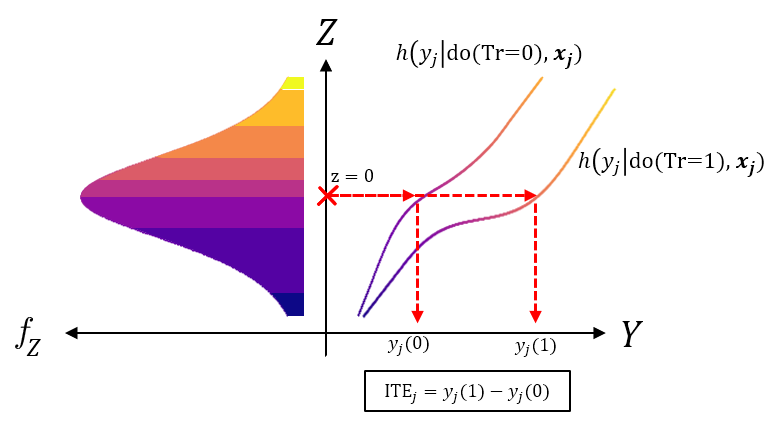
\includegraphics[width=0.6\textwidth]{img/potential_outcomes_y.png}
% \caption{Quantile treatment effect (QTE) at the median with TRAM-DAGs. The two transformation functions represent the distributions of the potential outcomes under both treatmetns. For the QTE(0.5), the median of the latent distribution is evaluated on both transformation functions to determine the median-potential-ouotcomes. This is in contrast to the ITE based on the expected values of the potential outcomes.}
% \label{fig:exp4_potential_outcomes}
% \end{figure}
% 
% 
% 
% 
% \begin{algorithm}
% \caption{ITE Estimation (QTE) Using TRAM-DAG in Observational Data}
% \label{alg:ite_qte}
% \begin{algorithmic}[1]
% \State \textbf{Input:} Fitted TRAM-DAG, observational dataset with $n$ samples
% \For{each sample $j = 1$ to $n$}
%   \State \textbf{Step 1: Encode explanatory nodes}
%   \For{each explanatory node $X_i \in \{X_1, X_2, X_3, X_5, X_6\}$}
%     \State Compute latent value: $z_{ij} = h_i(x_{ij} \mid \text{pa}(x_{ij}))$
%   \EndFor
% 
%   \State \textbf{Step 2: Generate potential outcomes under treatment and control}
%   \For{$x_4 \in \{0, 1\}$} \Comment{Simulate both treatment states}
%     \State Fix $X_4 = x_4$ (intervention)
%     \State Sample $X_5$ and $X_6$ sequentially using $z_{ij}$ and inverse transformations
%     \State Sample potential outcome $y_j^{(x_4)}$ using $z_{7,i} = 0$ (median of the potential outcome distribution)
% 
%   \EndFor
% 
%   \State \textbf{Step 3: Compute QTE for individual $j$}
%   \State $\text{ITE}_j = \text{median}(y_j^{(1)}) - \text{median}(y_j^{(0)})$
% \EndFor
% \State \textbf{Output:} ITE estimates $\{\text{ITE}_j\}_{j=1}^n$
% \end{algorithmic}
% \end{algorithm}
% 
% 
% 
% 
% 
% \textbf{Validation of results: } In the data generating mechanism, along with the actually sampled values, the potential values under both treatments are also recorded and used to determine the true QTE (the ITE based on the 50 percent quantiles of the potential outcome distributions of each individual.)
% The results are displayed by densities of the estimated ITE, the scatterplots of the true vs. estimated ITE, the ITE-ATE plot with the difference in medians as ATE within subgroups to make it comparable to the estimated ITEs. Furthermore the average of all estimated and true (dgp) ITEs are presented in table format. We further calculate the ATE as the overall difference in medians in the RCT setting and compare it to the estimated values based on the ITEs, althogh if this comparison in terms of the mean of a difference in medians is valid we did not further proof. It should be rather regarded as information, but not as proof. The scatterplot of the true vs. estimated ITE poses the most important validation.


% Check if true? probably not entirely... in both, the RCT and in the Observational setting, also other models could be applied instead of TRAM-DAG. As long as all confounders are included in the model, we controll for the confounders and can get unbiased results. For example a T-learner Colr($Y \sim X_1 + X_2 + X_3$) (because Colr is basically what we did in the DGP) fitted on both treatment groups separately could be used to estimate the ITE in our proposed experiment. This might only be possible so easily as long as we do not assume additional interactions between the treatment and the mediators $X_5$ and $X_6$. If we would assume such interactions, we would have to include these in the model as well, which would make it more complex and possibliy requires to fit and apply multiple models. If there are no interactions with the mediators, they can be omitted, since we are interested in the total treatment effects and not in separating the effect (mediation analysis). But again, we can only omit if these variables do not contain additional information about treatment effect heterogeneity. The reasoning is because to estimate the total effect one should not control for mediators. (check if really true!!!)  However, the TRAM-DAG framework is well suited to also deal with mediators and calculate counterfactuals, therefore we think it is a good example to show its capabilities.


% Notes after Meeting 24.06.25: Depending on the problem, CATE in terms of expected values of potential outcomes might be more appropriate than QTE, but also QTE could be better. Depends. If we wanted the potential outcomes based on the expected values, we have two options. either sample latent values and evaluate inverse tranformation functions. from those two sample distributions calculate the means to get the expected potential outcomes. Lucas suggested that we could also use numerical integreation instead, then we would not have to sample.











% \begin{table}
% 
% \caption{Comparison of confidence intervals for the mean differences across scenarios. The first row of each pair corresponds to the confidence interval from the linear model (lm), while the second row corresponds to the bootstrap method.}
% \centering
% \begin{tabular}[t]{lrr}
% \toprule
%   & Lower Bound & Upper Bound\\
% \midrule
% Scenario 1 (lm) & -0.58231 & -0.54359\\
% Scenario 1 (bootstrap) & -0.58210 & -0.54355\\
% Scenario 2 (lm) & -0.59118 & -0.55371\\
% Scenario 2 (bootstrap) & -0.59091 & -0.55405\\
% Scenario 3 (lm) & -0.06784 & -0.02799\\
% \addlinespace
% Scenario 3 (bootstrap) & -0.06784 & -0.02752\\
% \bottomrule
% \end{tabular}
% \end{table}

 



\subsection{Results and Discussion}

First, we present the results for Scenario 4.1 (Section~\ref{sec:exp4_sc1}), which includes both direct and interaction effects of treatment. Then, we show the results for Scenario 4.2 (Section~\ref{sec:exp4_sc2}), which has a direct effect but no interaction effects, and finally Scenario 4.3 (Section~\ref{sec:exp4_sc3}), which includes interaction effects but no direct treatment effect. For each scenario, we compare the results in an observational setting with confounded treatment allocation and in a randomized controlled trial (RCT) setting without confounding. We also compare the average treatment effect (ATE), which can be directly calculated in the RCT setting on observed outcomes, with the ATE derived from the estimated ITEs. All ITEs presented in this experiment are technically quantile treatment effects (QTEs), as defined in Equation~\ref{eq:qte}, based on the medians of the potential outcomes. For simplicity, we will refer to them as ITEs. The aim is to investigate how the TRAM-DAG performs in the presence or absence of direct and interaction effects of the treatment, both in confounded and in randomized settings, for the purpose of ITE estimation.

\subsubsection{Scenario 4.1: Direct and interaction effects} \label{sec:exp4_sc1}


\begin{figure}[H]
\centering
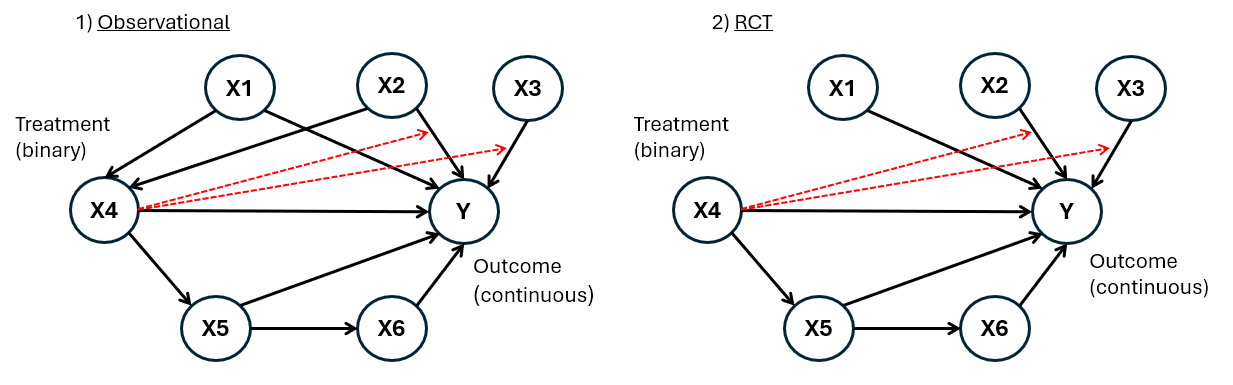
\includegraphics[width=0.85\textwidth]{img/exp4_dags.png}
\caption{DAGs for Scenario~4.1, which includes a direct effect of the treatment on the outcome and additional interaction effects with covariates $X_2$ and $X_3$. These DAGs were previously shown in Figure~\ref{fig:ite_dag_observational} and are re-plotted here for convenience. Left: Observational; Right: RCT setting.}
\label{fig:ite_dag_observational_1}
\end{figure}

Scenario~4.1 includes a direct effect of the treatment on the outcome, and interaction effects with $X_2$ and $X_3$, as shown in Figure~\ref{fig:ite_dag_observational_1}.

In the observational setting, treatment was confounded by $X_1$ and $X_2$. In the train set, $38.6$\% of individuals were in the control group and $61.4$\% in the treatment group. The test set had a similar distribution.

In the RCT setting, treatment was randomly assigned. In the train set, $49.8$\% were in control and $50.2$\% in treatment; in the test set, the shares were $50.2$\% and $49.8$\%, respectively.

Figure~\ref{fig:scenario1_ite_distribution_dgp} shows the true ITE distribution resulting from the DGP, which displays some heterogeneity due to interaction effects. Figure~\ref{fig:scenario1_sampling_distributions_vertical} shows the marginal distributions of all variables in the DGP and as estimated by the TRAM-DAG. The distribution of the outcome $Y$ under $\text{do}(X_4 = 0)$ and $\text{do}(X_4 = 1)$ is shown in Figure~\ref{fig:scenario1_outcome_distributions}. The ITEs were estimated as the difference in medians of the potential outcomes. Figure~\ref{fig:scenario1_ite_densities_train_test} compares the densities of the estimated and true ITEs. Figure~\ref{fig:scenario1_ite_scatter_train_test} shows the scatterplots of estimated vs. true ITEs. In both observational and RCT settings, the estimated ITEs are close to the true ones in both train and test sets. Figures~\ref{fig:observ_scenario1_ite_ATE} and \ref{fig:rct_scenario1_ite_ATE} show the ITE-ATE plots, where the ATE is calculated as the median difference in observed outcomes within ITE subgroups. The trends are similar across train and test sets and follow the calibration line.



The ATEs calculated based on different measures in both the training and test sets are shown in Table~\ref{tab:scenario1_ate_comparison}. In the RCT setting (training set), the difference in means of the outcomes between the two treatment groups was 
$-0.563$, with a 95\% Wald confidence interval from 
$-0.582$ to 
$-0.543$. Note that the ATE in terms of difference in means cannot be directly compared to the ATE based on difference in medians.



% 
% Scenario (1) included a direct effect of the treatment on the outcome and an additional interaction effect of the treatment with the covariates X2 and X3, as presented in Figure~\ref{fig:ite_dag_observational_1}. A train and test set were generated with 20,000 observations each. 
% In the observational setting, the treatment allocation was confounded by the covariates X1 and X2.  In the train set, $round(observ_scenario1$dev_treatment_allocation[1]*100, 1)$\% of patients were in the control group and $round(observ_scenario1$dev_treatment_allocation[2]*100, 1)$\% were in the treatment group. This ratio was similar in the test set. 
% In the RCT setting treatment allocation was randomized. In the train set $round(rct_scenario1$dev_treatment_allocation[1]*100, 1)$\% individuals were in the control group and $round(rct_scenario1$dev_treatment_allocation[2]*100, 1)$\% in the treatment group. In the test set $round(rct_scenario1$val_treatment_allocation[1]*100, 1)$\% were in the control group and $round(rct_scenario1$val_treatment_allocation[2]*100, 1)$\% in the treatment group. 
% Figure \ref{fig:scenario1_ite_distribution_dgp} illustrates the true ITE distribution that resulted from the DGP. Due to the interaction effects, there is some heterogeneity in the ITE distribution. Figure \ref{fig:scenario1_sampling_distributions_vertical} shows the marginal distributions of all variables according to the DGP and the estimates by the fitted TRAM-DAG. Figure \ref{fig:scenario1_outcome_distributions} shows the distribution of the outcome ($Y$) under the do(Tr=0) and do(Tr=1) interventions. The fitted model was applied to estimate the ITEs in terms of the difference in medians of the potential outcomes. The resulting density of the estimated ITEs compared to the true ITEs according to the DGP is shown in Figure \ref{fig:scenario1_ite_densities_train_test}. Across both settings, the densities of the estimated ITEs are close to the true densities in both the training and test datasets. Figure \ref{fig:scenario1_ite_scatter_train_test} shows the scatterplots of true against estimated ITEs. Finally, Figure \ref{fig:scenario1_ite_cATE} displays the ITE-ATE plot where the ATE is computed as the difference in medians of the observed outcome under the treatments within the respective ITE-subgroups. The trends observed in the training and test sets are consistent.


% The average treatment effect (ATE) is presented in Table \ref{tab:scenario1_ate_comparison}. In the RCT setting in the training set, the difference in means of the outcomes in the two treatment groups was $round(rct_scenario1$dev_ATE_observed_Y_mean_diff, 3)$ with a confidence interval of $round(rct_scenario1$dev_ATE_observed_Y_mean_diff_CI[1], 3)$ to $round(rct_scenario1$dev_ATE_observed_Y_mean_diff_CI[2], 3)$. The ATEs calculated based on different measuress in the training and test dataset, are shown in Table \ref{tab:scenario1_ate_comparison}.


% The ATE in terms of the difference in medians of the observed outcomes was $round(rct_scenario1$dev_ATE_observed_Y_median_diff, 3)$. Also in the training set, the ATE in terms of the mean of the true ITEs was $round(rct_scenario1$dev_ITE_median_average, 3)$ and the ATE in terms of the mean of the estimated ITEs was $round(rct_scenario1$dev_ITE_median_pred_average, 3)$. 


\begin{table}[htbp]
\centering
\small
\caption{Scenario~4.1, including direct and interaction effects: Comparison of ATE measures across training and test sets for the observational and RCT settings. $\text{Y}_\text{observed}^{(\text{Tr})}$ denotes the observed outcome under the treatment ($\text{Tr}$) actually received. Estimates based on these observed outcomes (means and medians) are provided only for the RCT setting, as the observational setting is confounded. The true ITEs ($\text{ITE}_\text{true}$) were calculated for each individual based on the data-generating process. In contrast, the estimated ITEs ($\text{ITE}_\text{estimated}$) were obtained from the TRAM-DAG trained on observed data. The estimated ATE from $\text{mean}(\text{ITE}_\text{estimated})$ can be directly compared to the true $\text{mean}(\text{ITE}_\text{true})$, whereas comparisons to empirical ATEs from observed outcome differences should be interpreted with caution. All ITEs were computed as quantile treatment effects (QTEs) based on the median of the potential outcome distributions, as defined in Equation~\ref{eq:qte}.}
\label{tab:scenario1_ate_comparison}
\begin{tabular}{l c c c c}
\toprule
\textbf{Measure} & \multicolumn{2}{c}{\textbf{Observational}} & \multicolumn{2}{c}{\textbf{RCT}} \\
\cmidrule(lr){2-3} \cmidrule(lr){4-5}
 & \textbf{Train} & \textbf{Test} & \textbf{Train} & \textbf{Test} \\
\midrule
ATE as $\text{mean}(\text{Y}_\text{observed}^{(1)}) - \text{mean}(\text{Y}_\text{observed}^{(0)})$ 
& NA & NA 
& -0.563 
& -0.563 \\

ATE as $\text{median}(\text{Y}_\text{observed}^{(1)}) - \text{median}(\text{Y}_\text{observed}^{(0)})$  
& NA & NA 
& -0.626 
& -0.638 \\

ATE as mean(ITE$_\text{true}$)  
& -0.620 
& -0.622 
& -0.620 
& -0.622 \\

ATE as mean(ITE$_\text{estimated}$) 
& -0.617 
& -0.620 
& -0.619 
& -0.622 \\
\bottomrule
\end{tabular}
\end{table}

% 
% \begin{table}[htbp]
% \centering
% \small
% \caption{Scenario (1), including direct and interaction effects: Comparison of ATE measures across train and test sets for the observational and RCT setting.}
% \label{tab:scenario1_ate_comparison_old}
% \begin{tabular}{l c c c c}
% \toprule
% \textbf{Measure} & \multicolumn{2}{c}{\textbf{Observational}} & \multicolumn{2}{c}{\textbf{RCT}} \\
% \cmidrule(lr){2-3} \cmidrule(lr){4-5}
%  & \textbf{Train} & \textbf{Test} & \textbf{Train} & \textbf{Test} \\
% \midrule
% ATE as $\text{mean}(\text{Y}_\text{observed}^{(1)}) - \text{mean}(\text{Y}_\text{observed}^{(0)})$ & NA & NA & round(rct_scenario1$dev_ATE_observed_Y_mean_diff, 3) & round(rct_scenario1$val_ATE_observed_Y_mean_diff, 3) \\
% ATE as $\text{median}(\text{Y}_\text{observed}^{(1)}) - \text{median}(\text{Y}_\text{observed}^{(0)})$  & NA & NA & round(rct_scenario1$dev_ATE_observed_Y_median_diff, 3) & round(rct_scenario1$val_ATE_observed_Y_median_diff, 3) \\
% ATE as mean(ITE$_\text{true}$)  & round(observ_scenario1$dev_ITE_median_average, 3) & round(observ_scenario1$val_ITE_median_average, 3) & round(rct_scenario1$dev_ITE_median_average, 3) & round(rct_scenario1$val_ITE_median_average, 3) \\
% ATE as mean(ITE$_\text{estimated}$) & round(observ_scenario1$dev_ITE_median_pred_average, 3) & round(observ_scenario1$val_ITE_median_pred_average, 3) & round(rct_scenario1$dev_ITE_median_pred_average, 3) & round(rct_scenario1$val_ITE_median_pred_average, 3) \\
% \bottomrule
% \end{tabular}
% \end{table}




\begin{figure}[htbp]
\centering
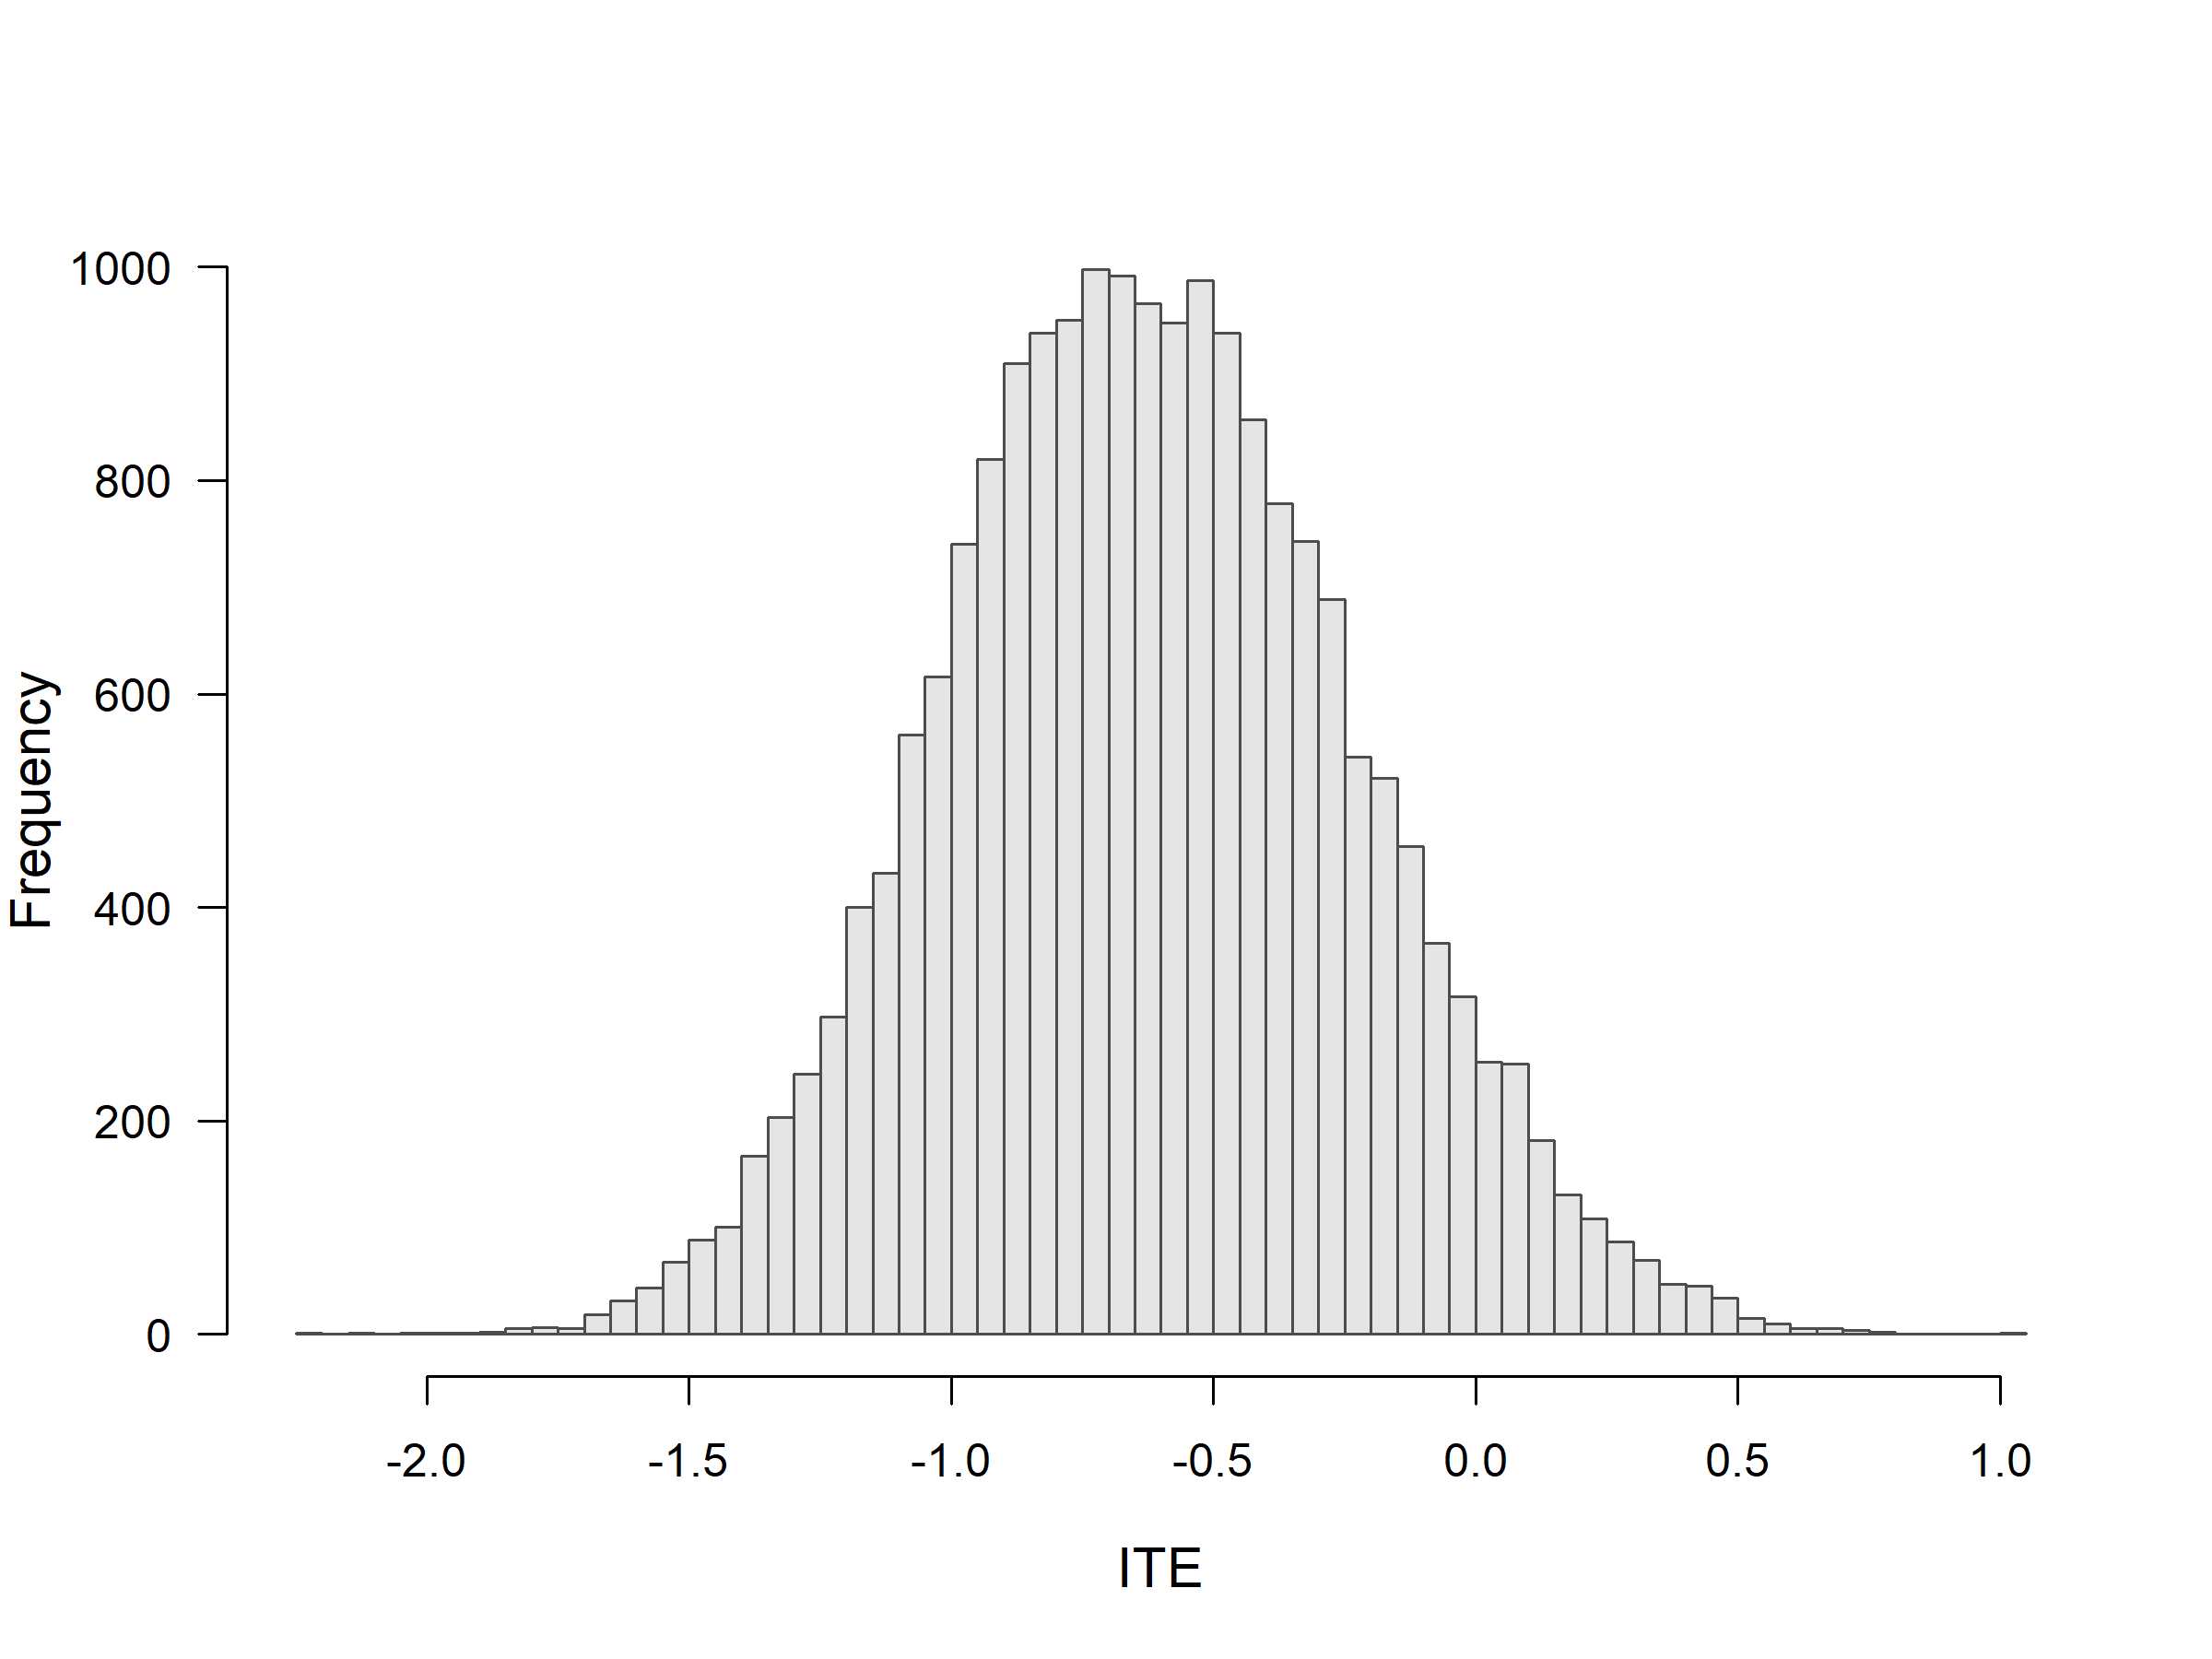
\includegraphics[width=0.7\textwidth]{img/results/observ_scenario1_ite_distribution_dgp.png}
\caption{True ITE distribution resulting from the DGP for Scenario 4.1, which includes both direct and interaction effects. The true ITEs are identical for each individual in the observational and RCT settings, as they are based on the potential outcomes under both treatment conditions.}
\label{fig:scenario1_ite_distribution_dgp}
\end{figure}



\begin{figure}[htbp]
\centering
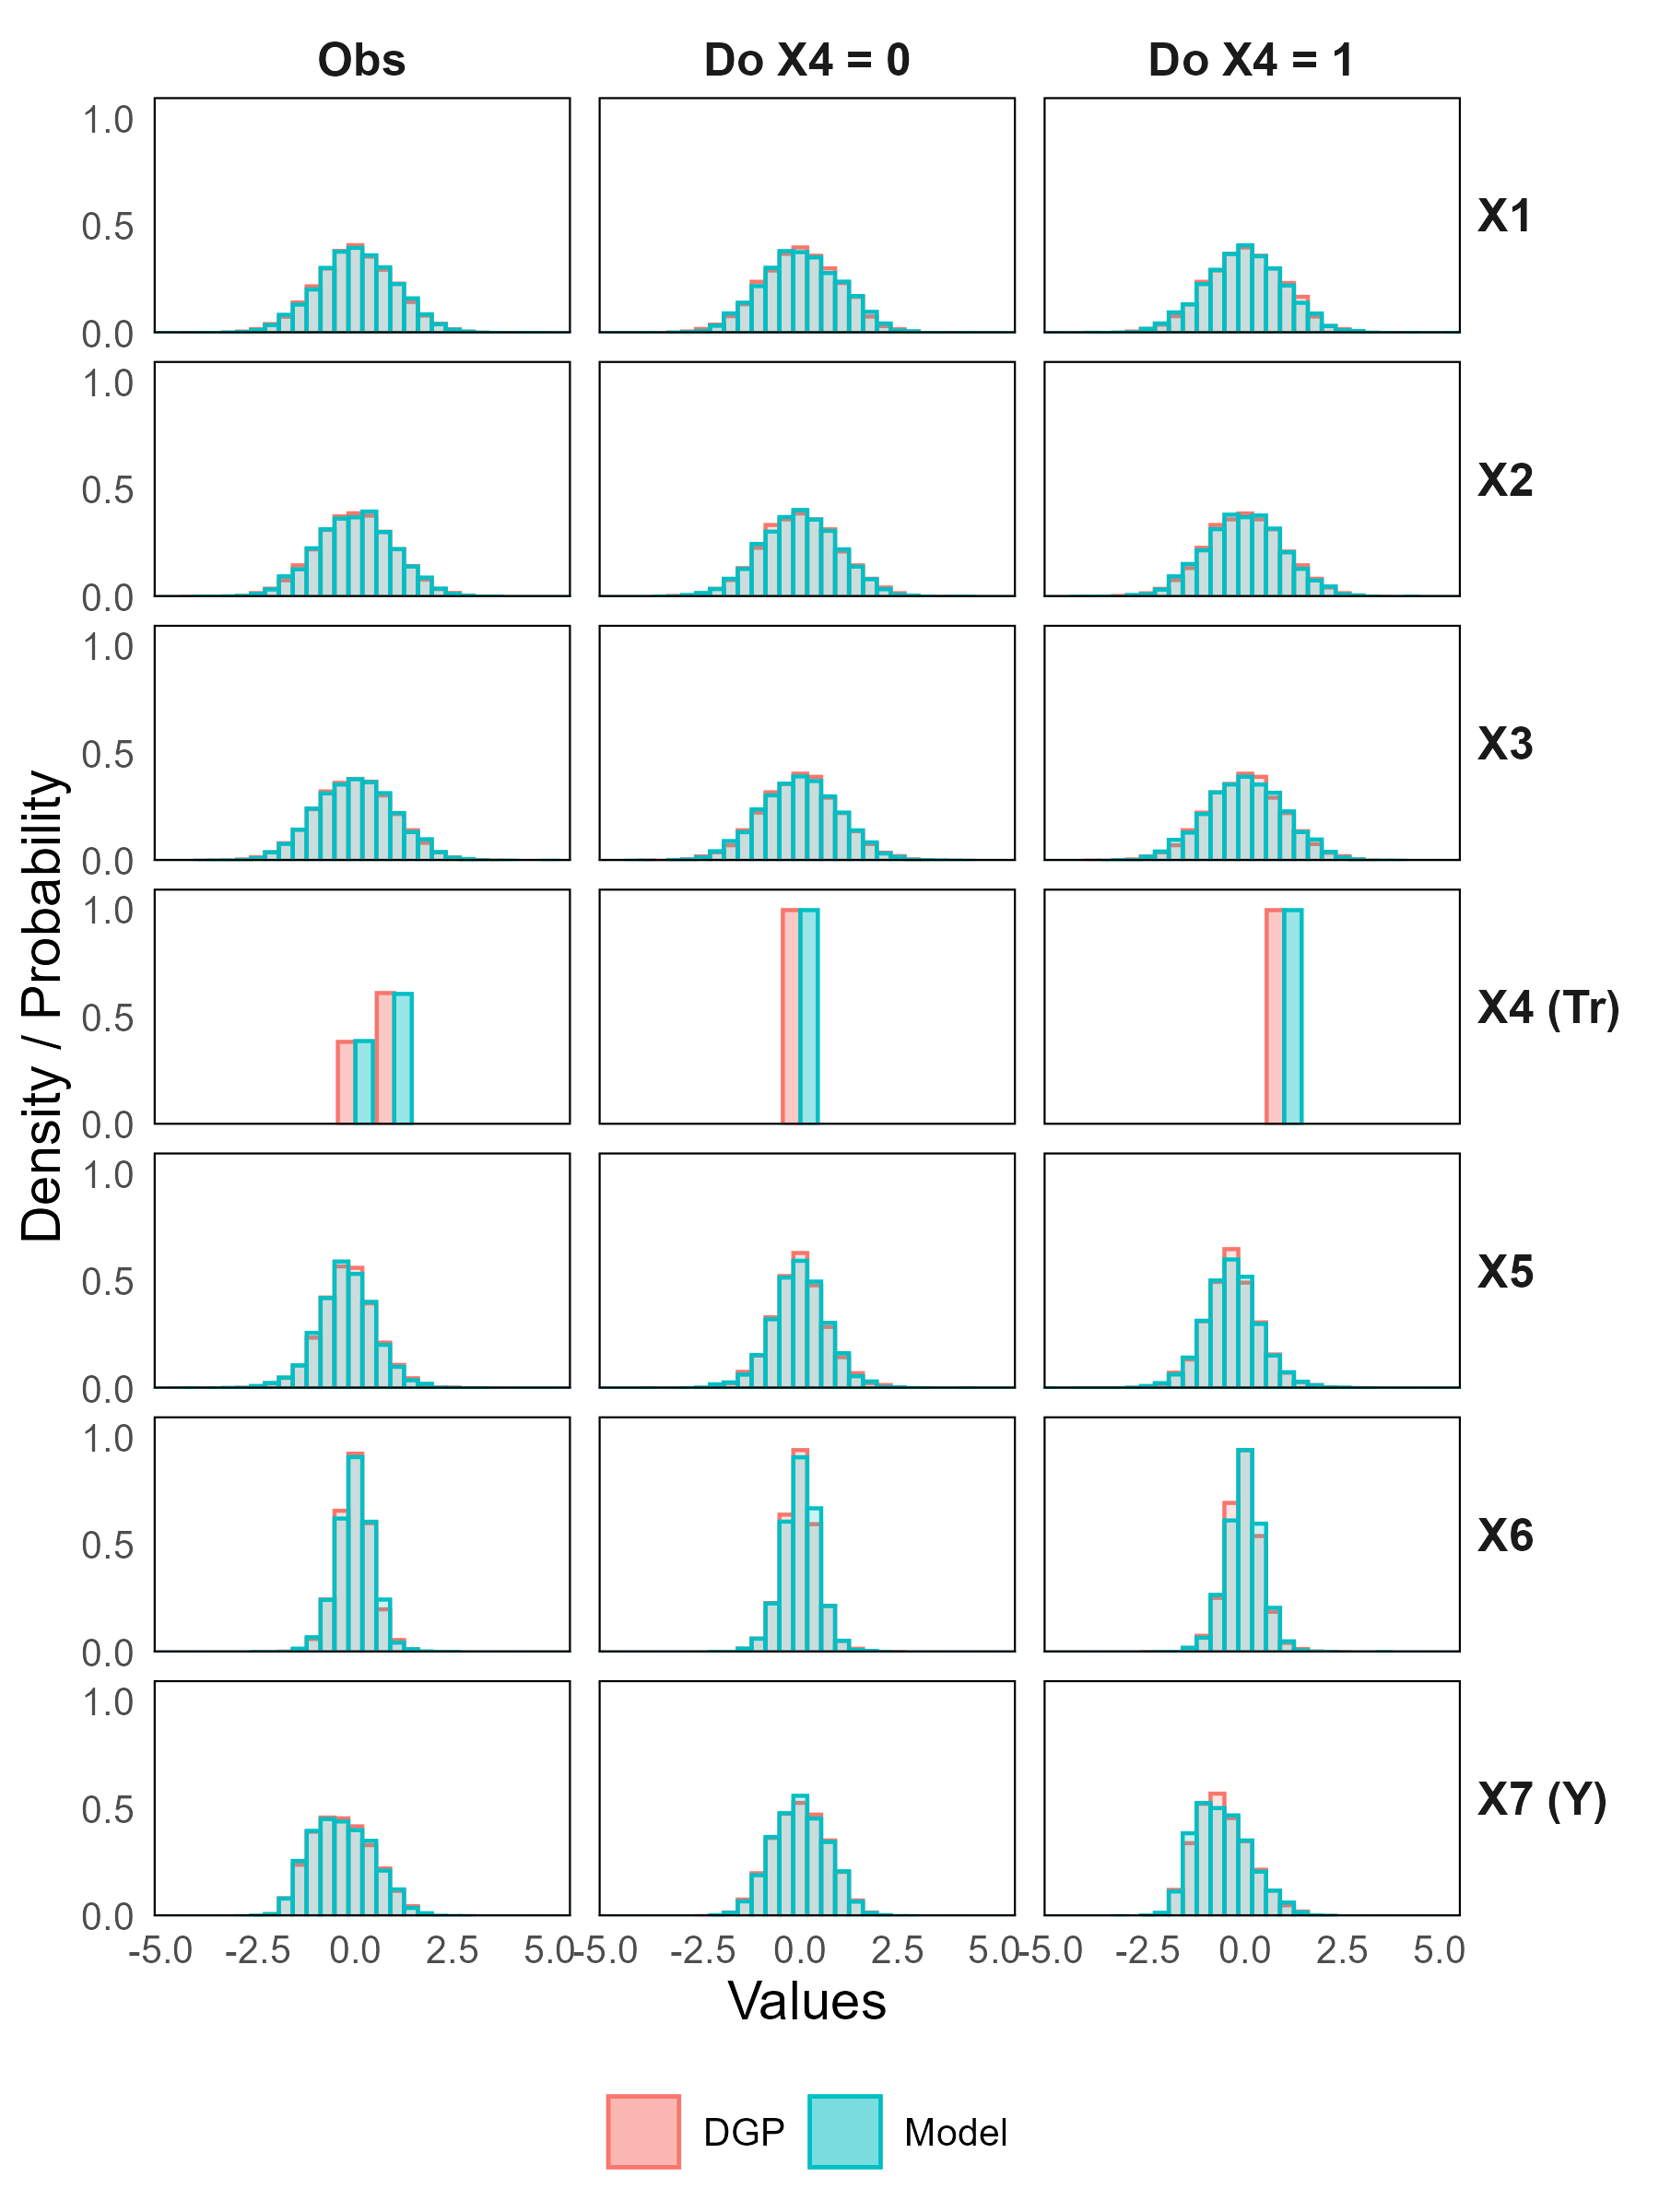
\includegraphics[width=0.45\textwidth]{img/results/observ_scenario1_sampling_distributions_vertical.png}
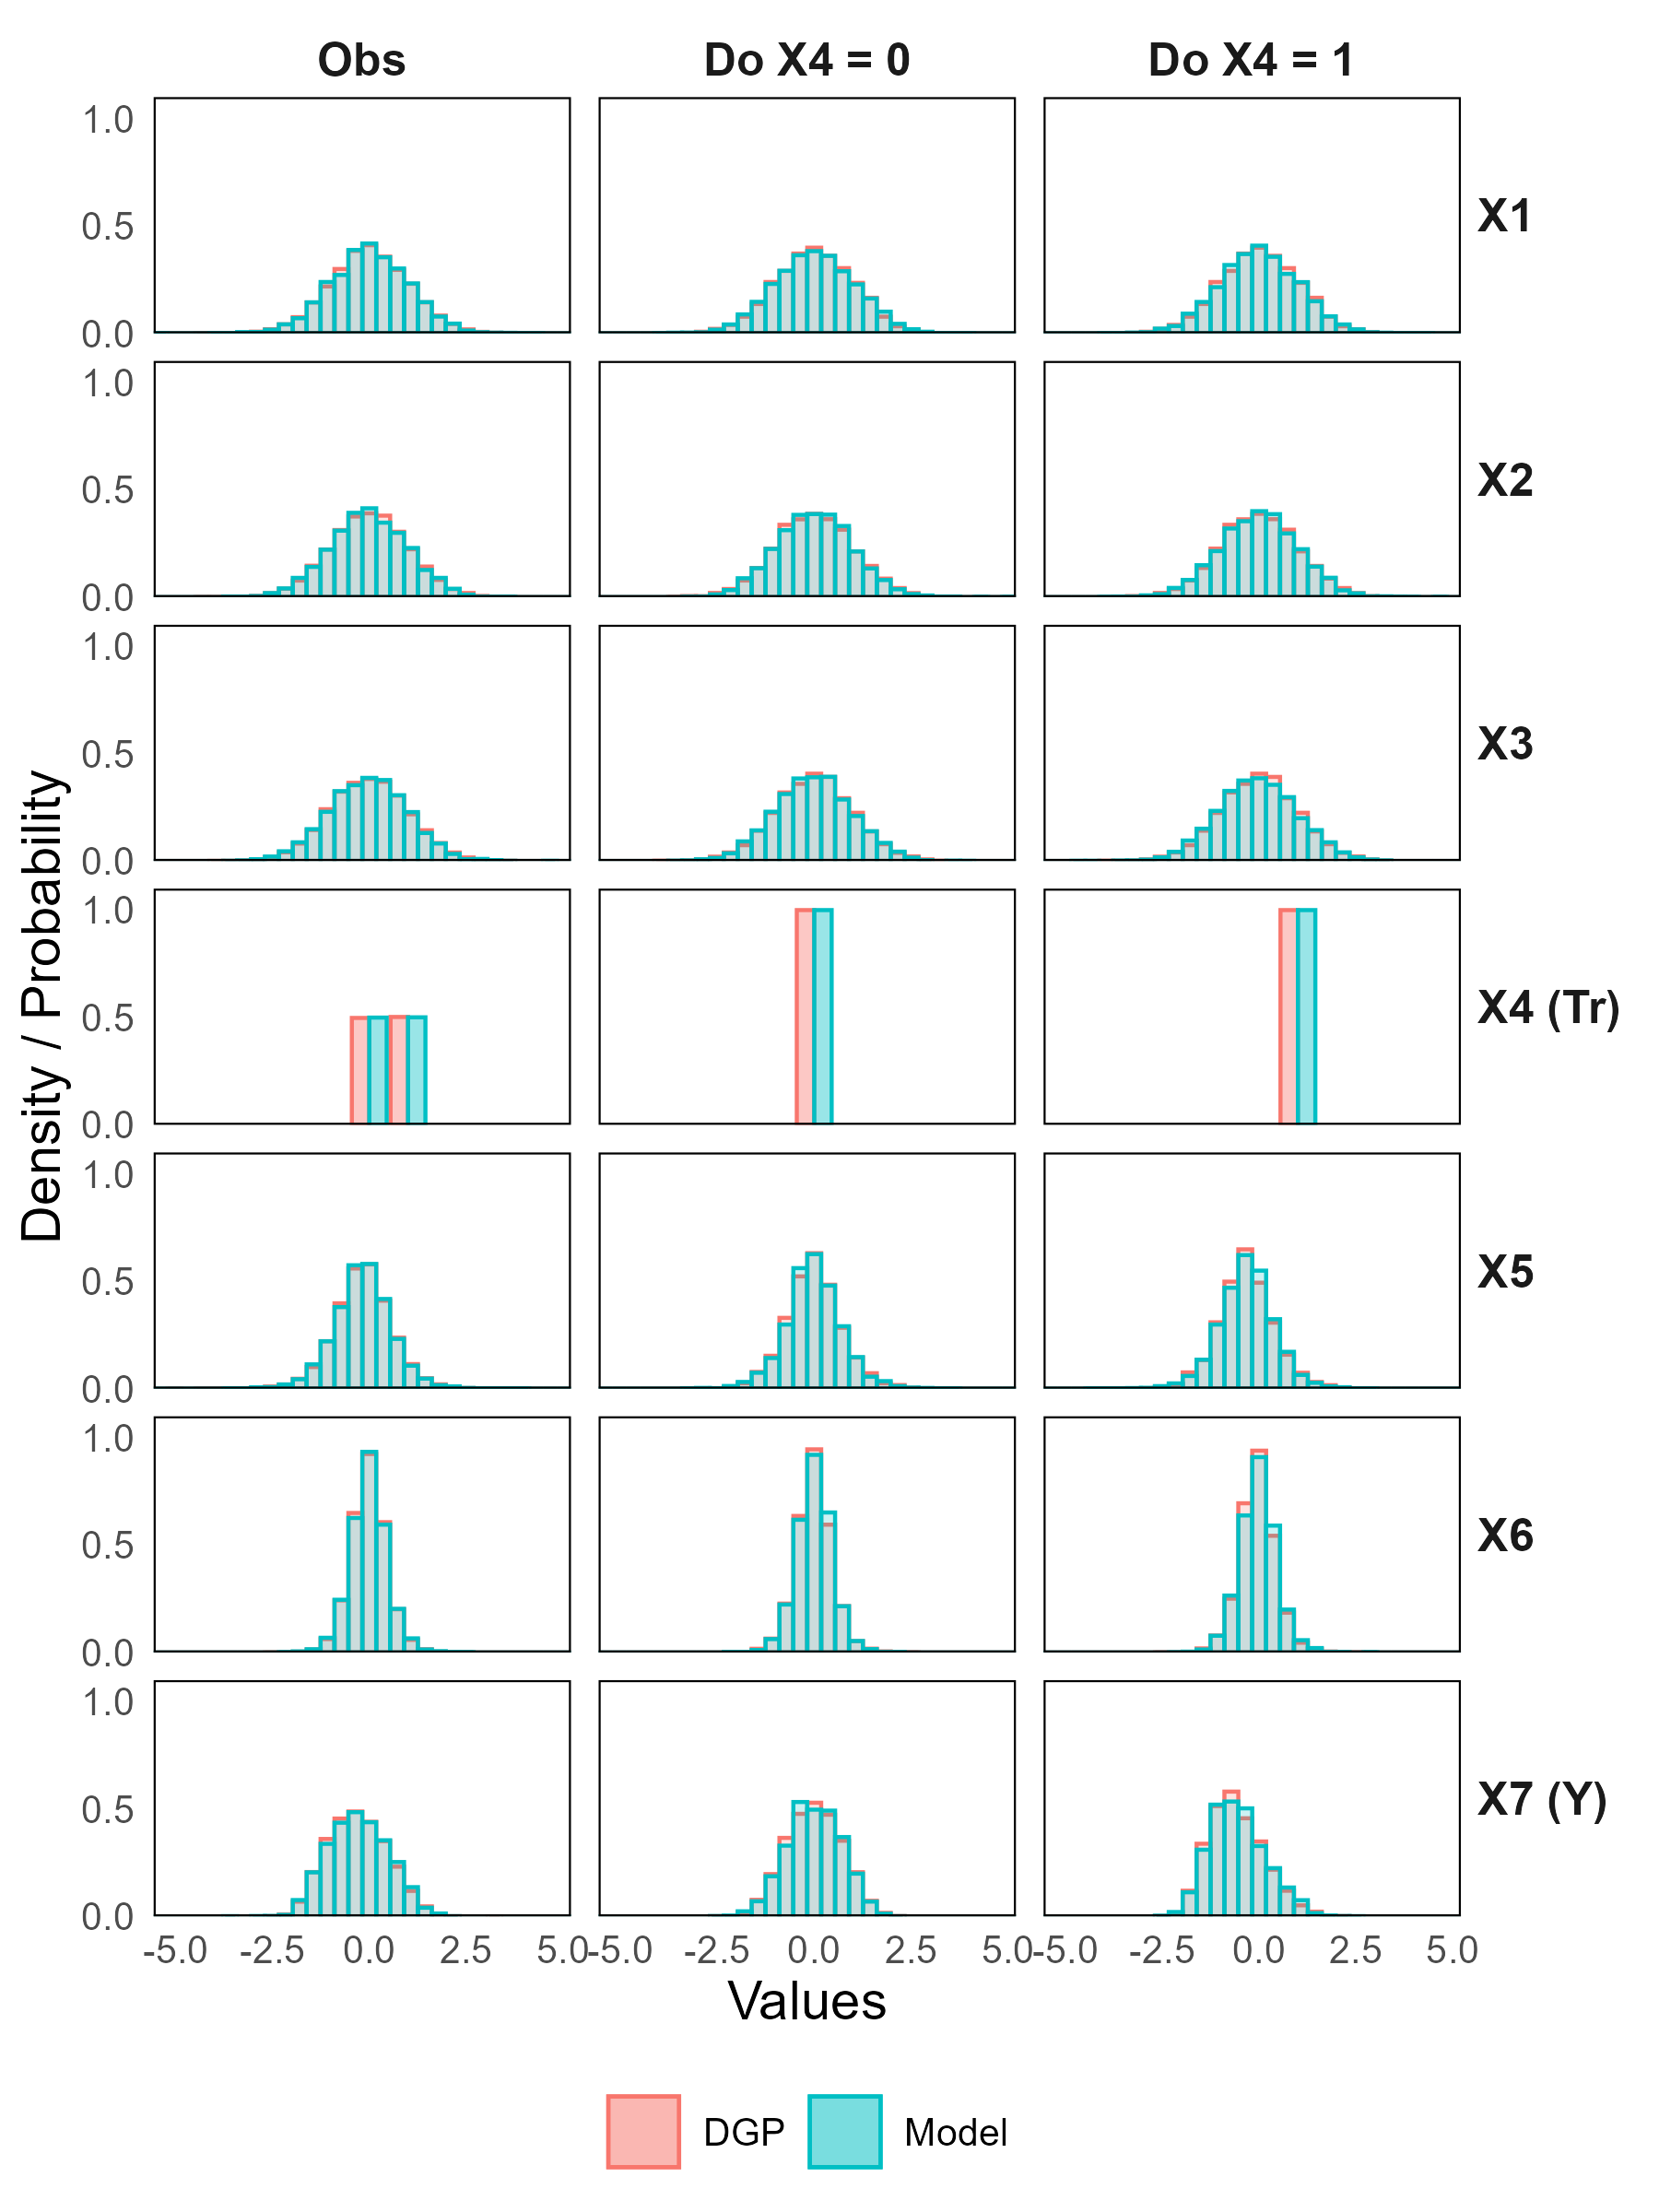
\includegraphics[width=0.45\textwidth]{img/results/rct_scenario1_sampling_distributions_vertical.png}
\caption{Marginal distributions of variables from the DGP and from samples generated by the fitted TRAM-DAG for Scenario 4.1 with direct and interaction effects. Distributions are shown as observed (Obs), under the control intervention do($X_4 = 0$), and under the treatment intervention do($X_4 = 1$). Left: Observational; Right: RCT setting.}
\label{fig:scenario1_sampling_distributions_vertical}
\end{figure}


\begin{figure}[htbp]
\centering
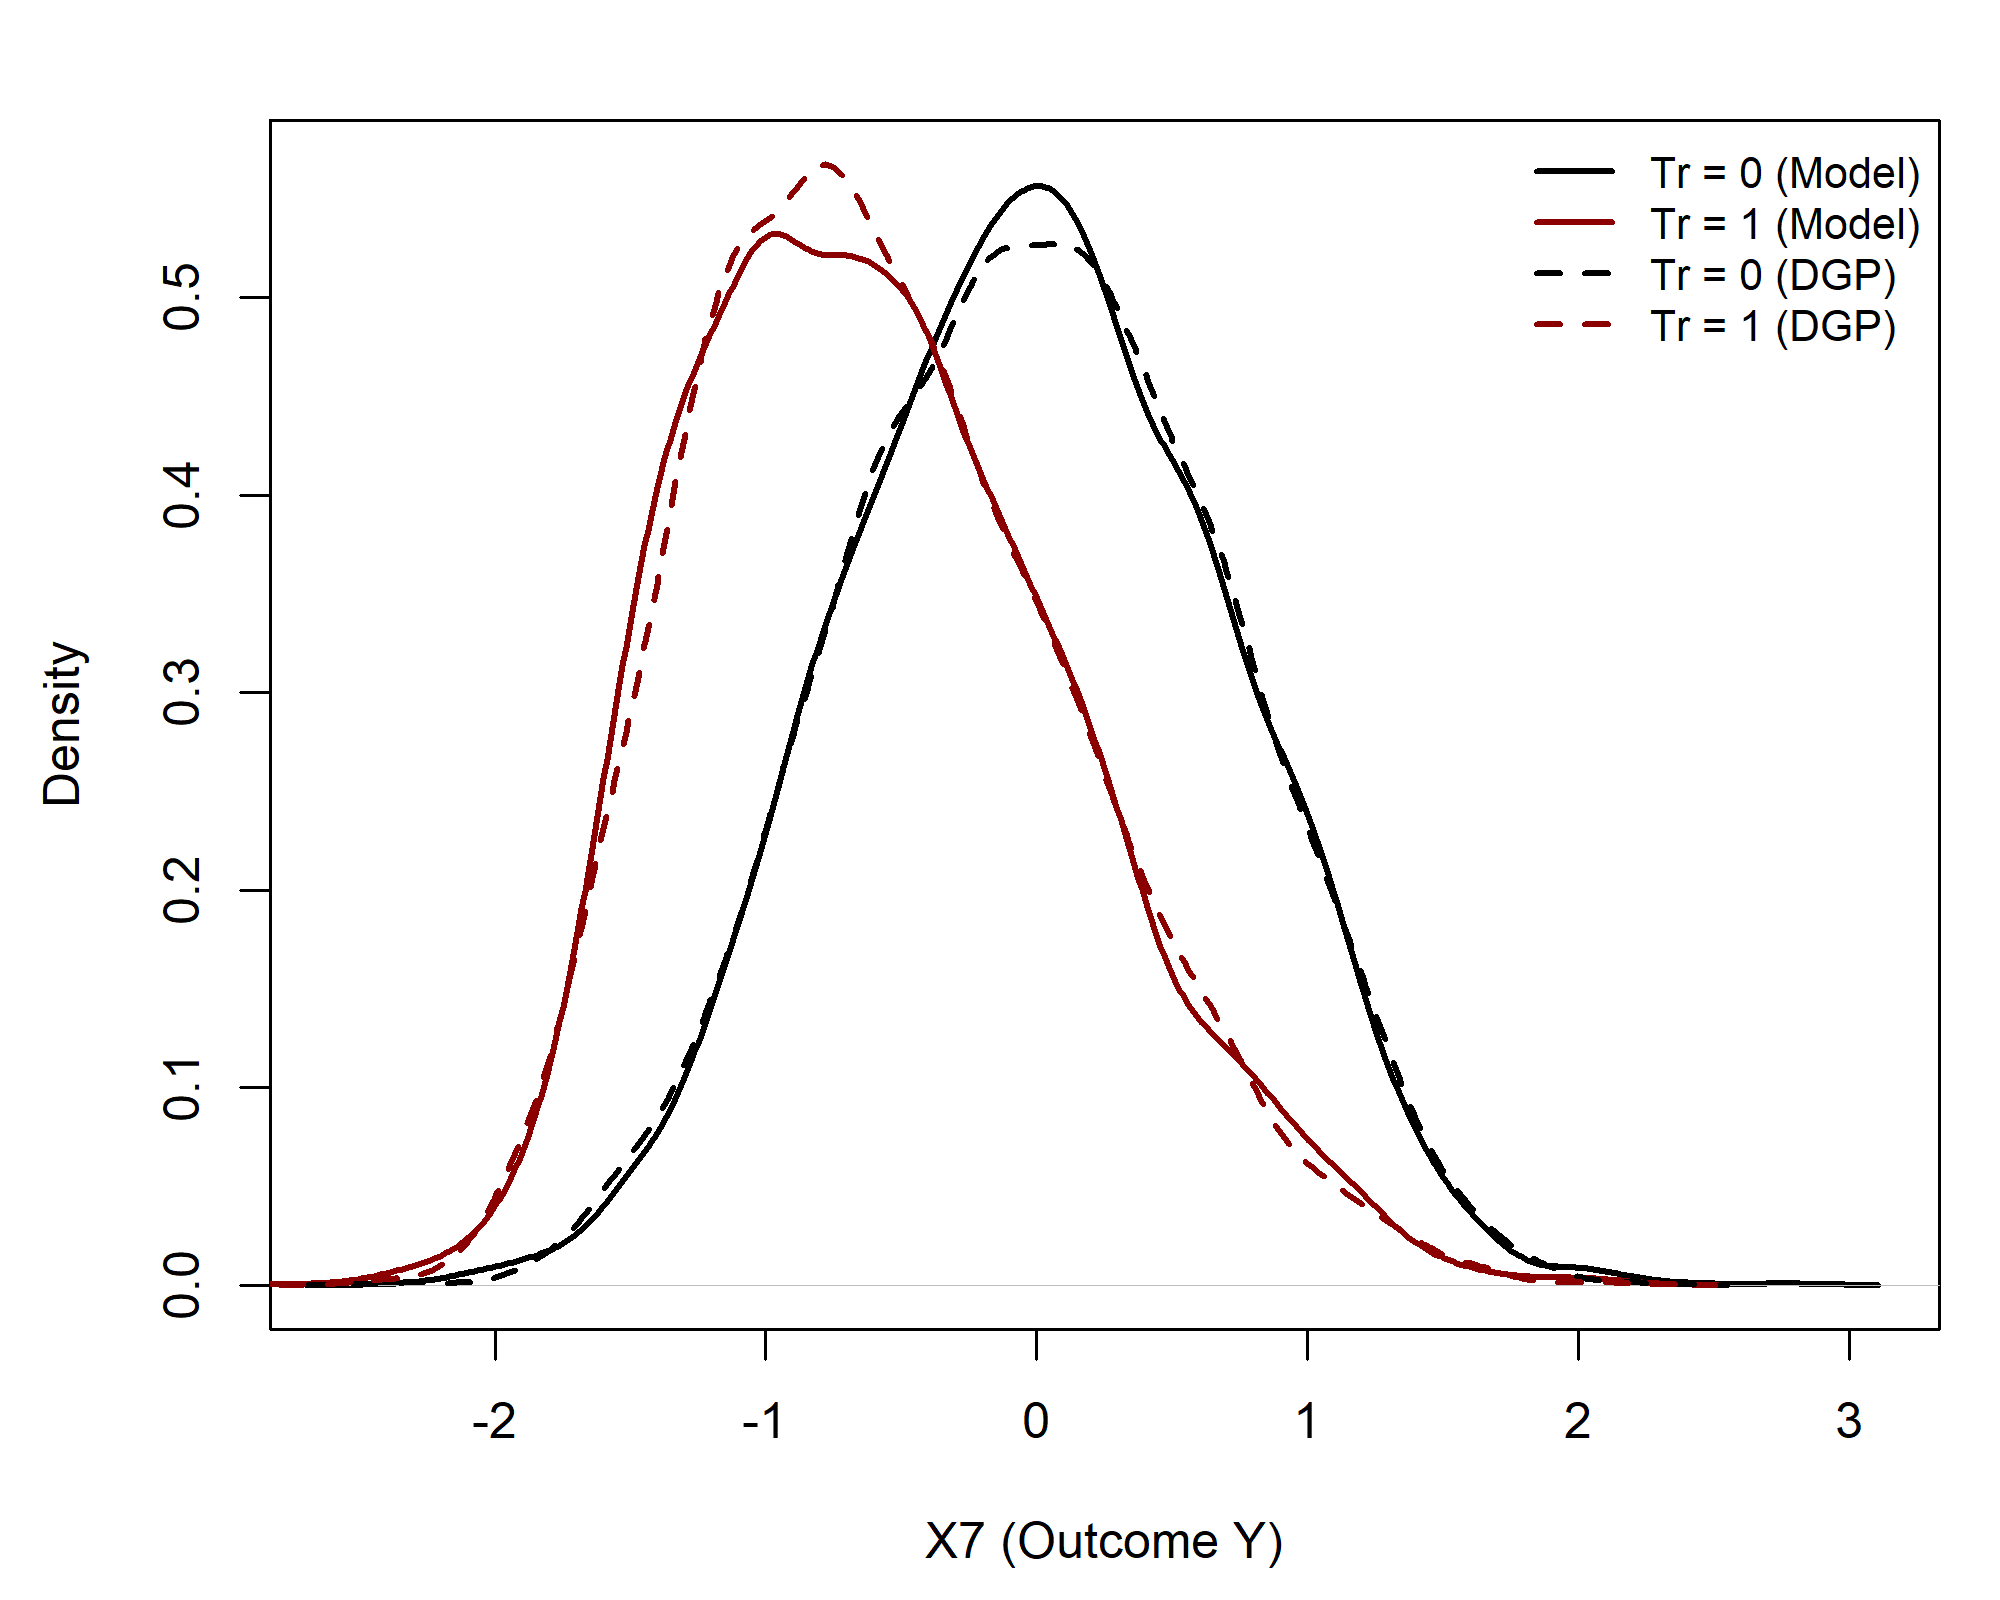
\includegraphics[width=0.45\textwidth]{img/results/observ_scenario1_X7_treatment_densities.png}
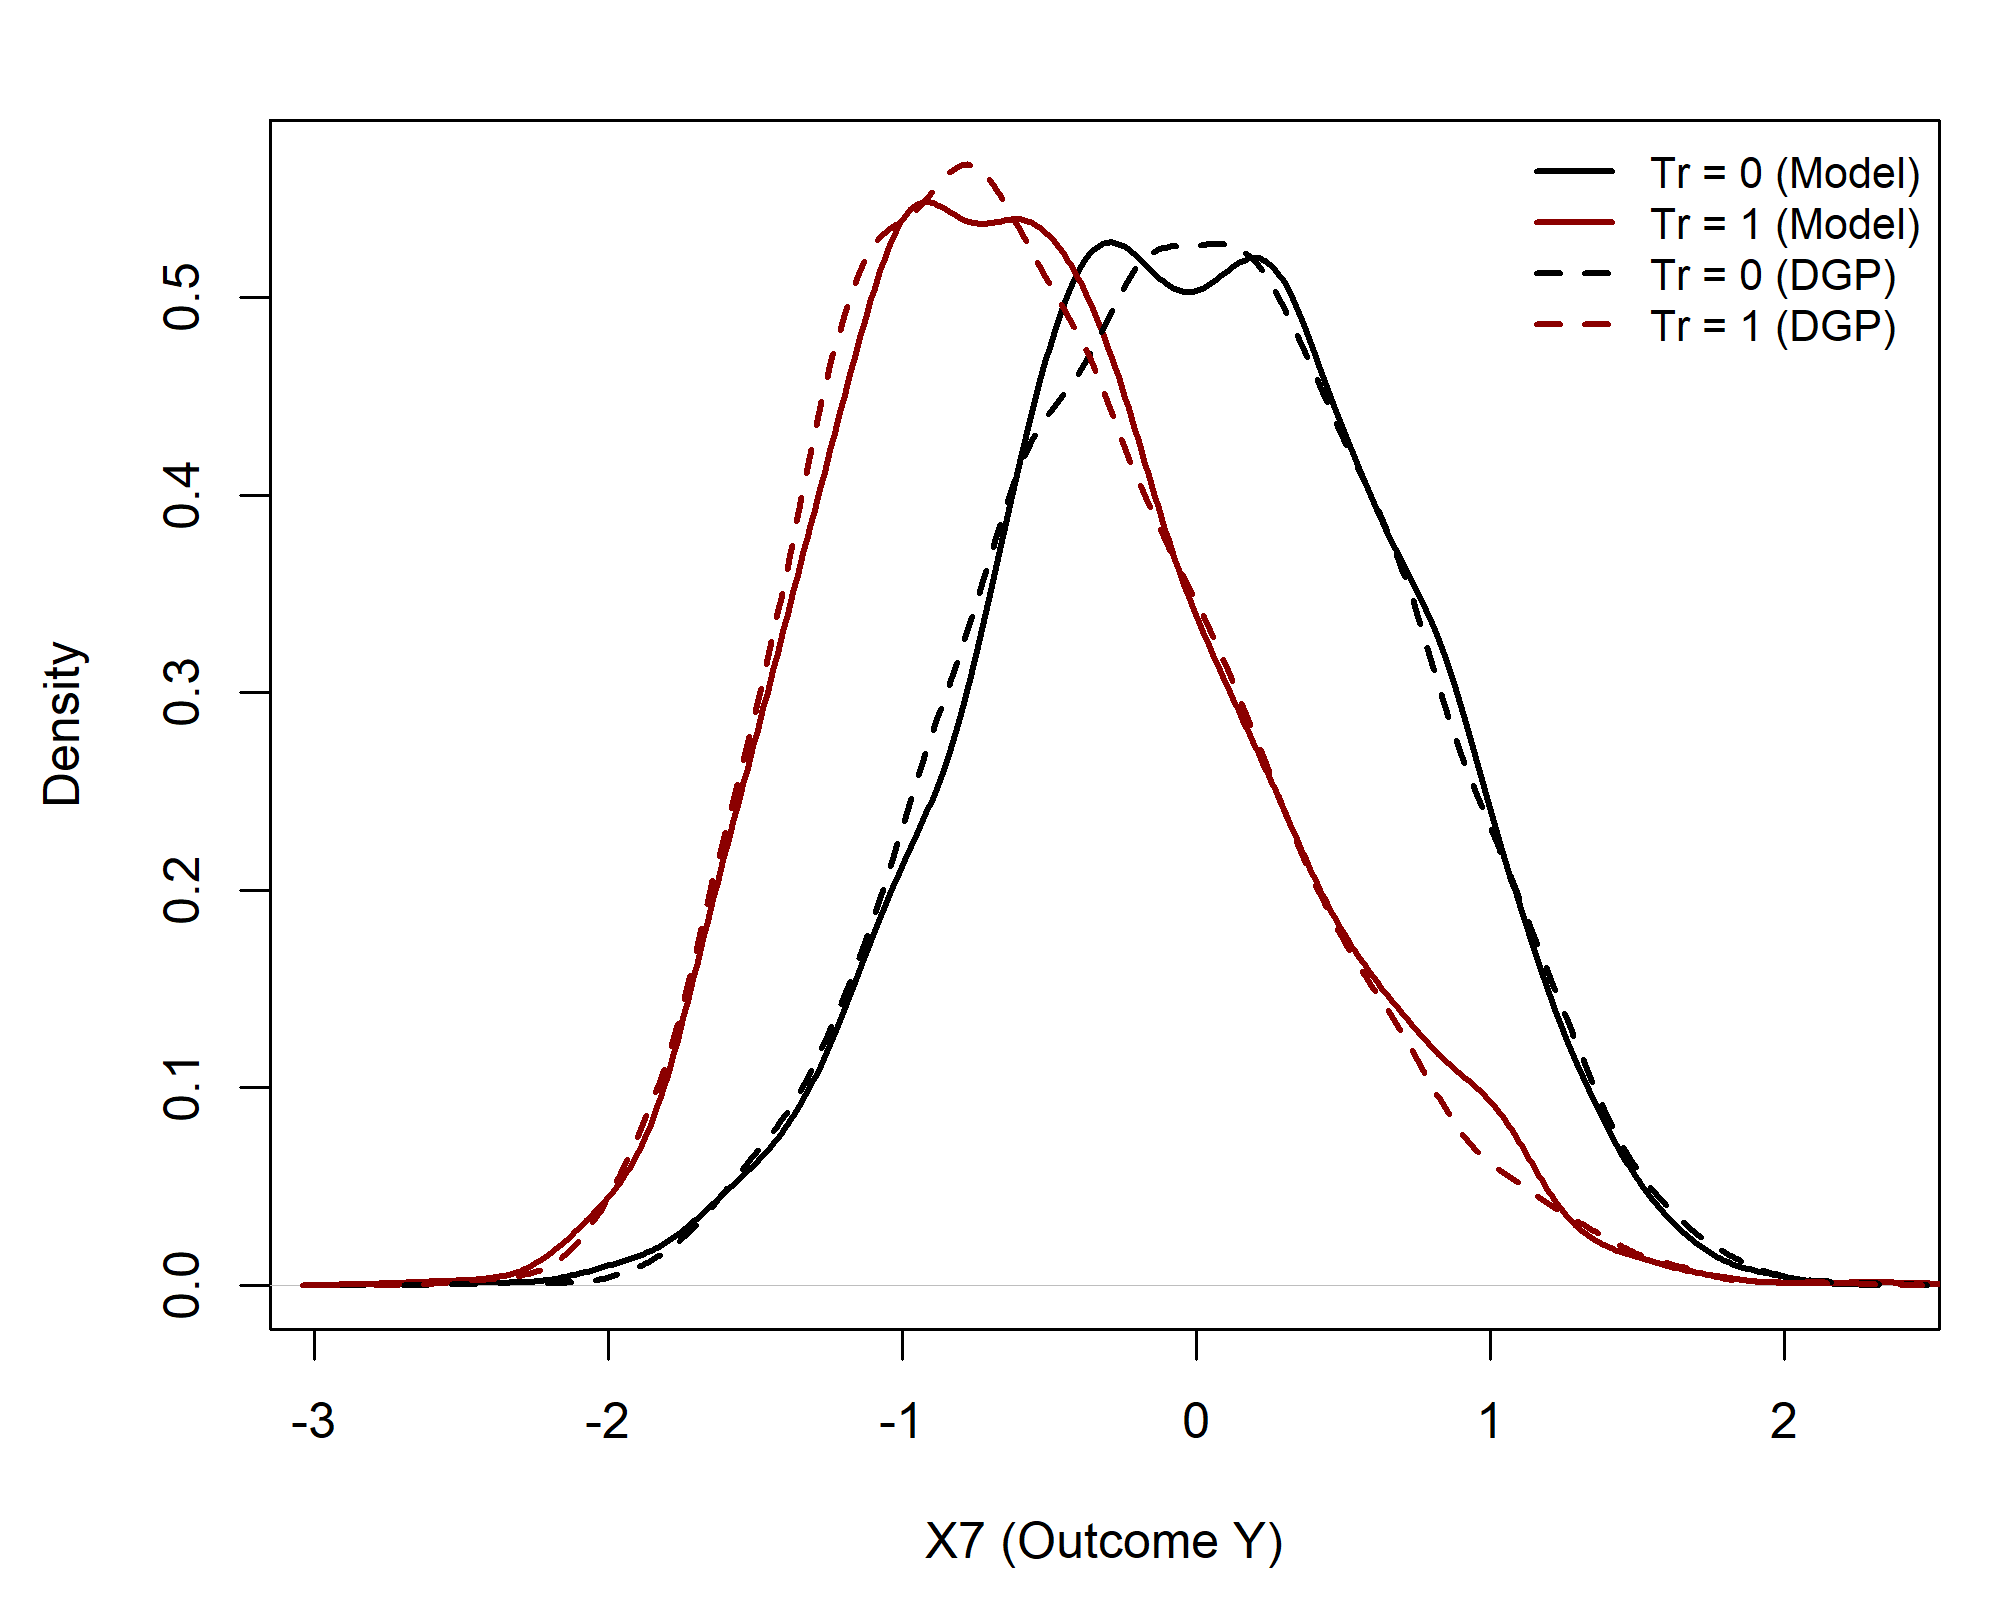
\includegraphics[width=0.45\textwidth]{img/results/rct_scenario1_X7_treatment_densities.png}
\caption{Distributions of the outcome variable ($X_7=Y$) under control and treatment interventions for Scenario 4.1, which includes both direct and interaction effects. This plot provides a more detailed view of the $X_7$ panels shown under do($X_4=0$) and do($X_4=1$) in Figure~\ref{fig:scenario1_sampling_distributions_vertical}. Left: Observational; Right: RCT setting.}
\label{fig:scenario1_outcome_distributions}
\end{figure}




\begin{figure}[htbp]
\centering
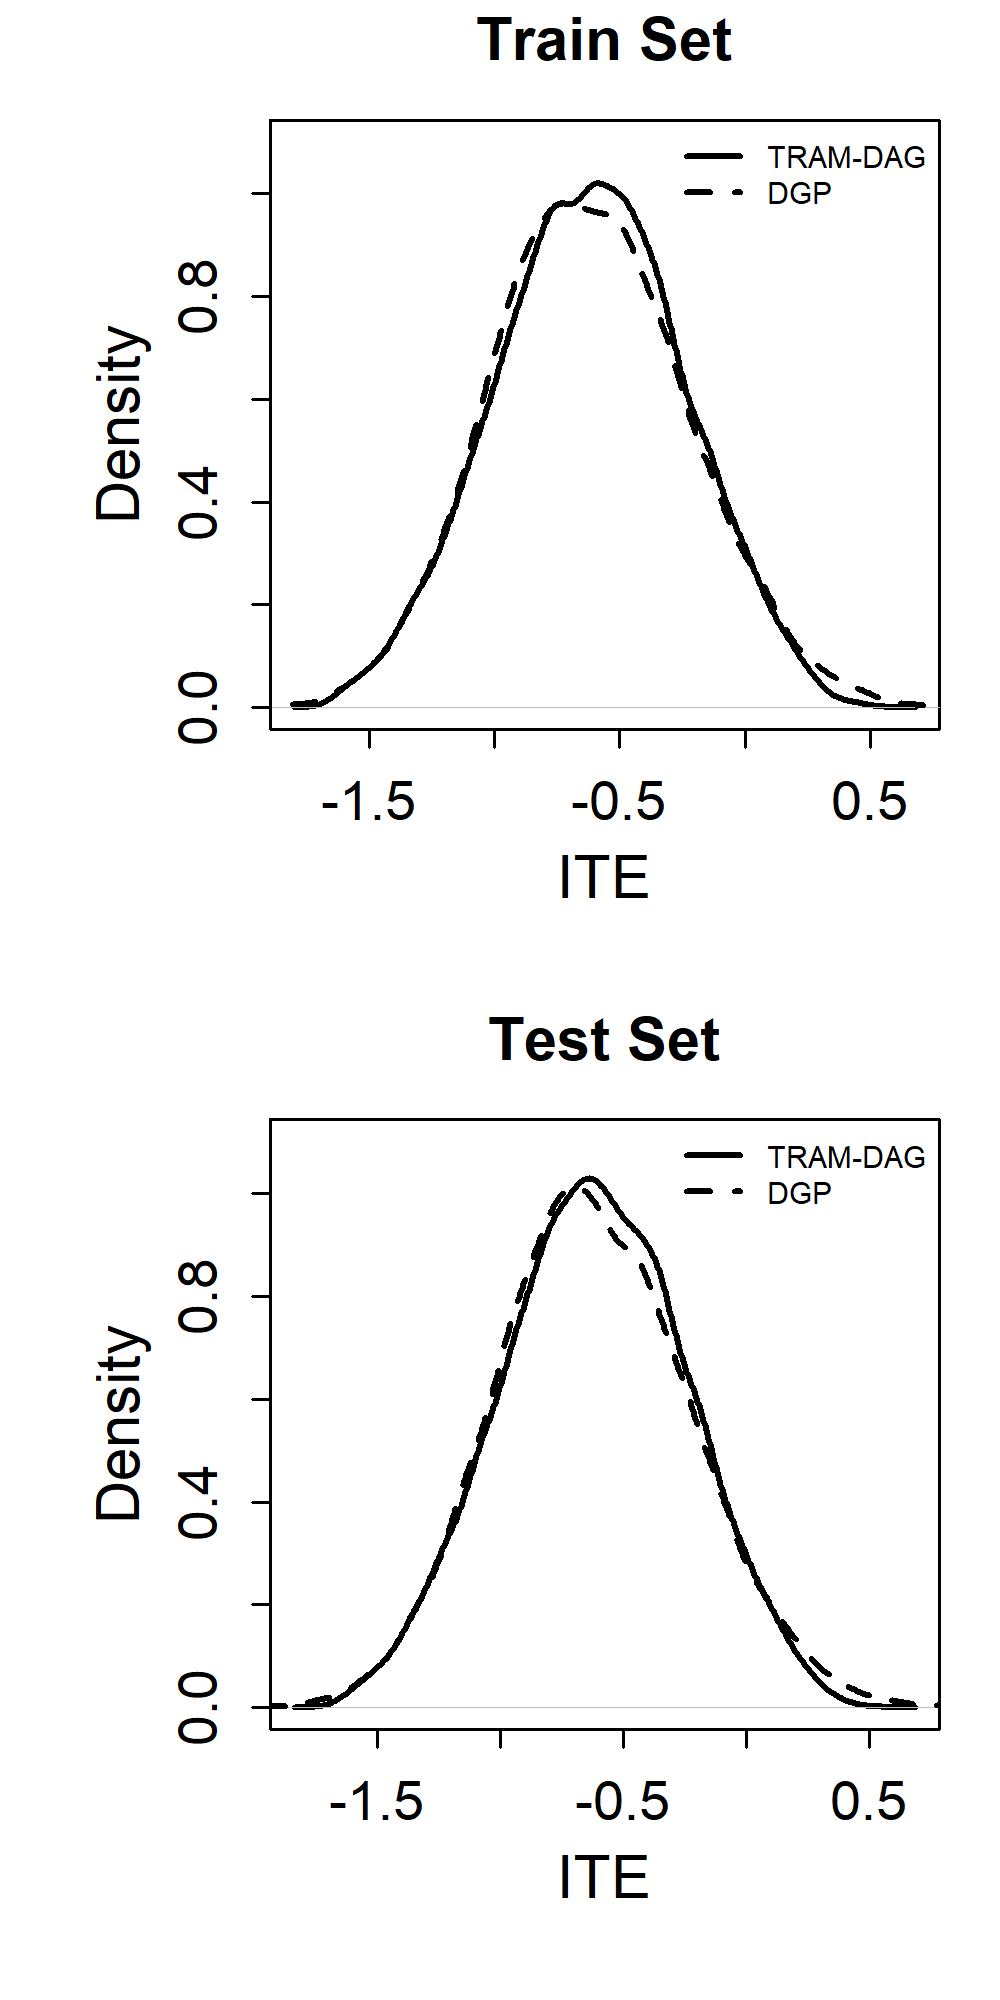
\includegraphics[width=0.33\textwidth]{img/results/observ_scenario1_ITE_densities_train_test.png} 
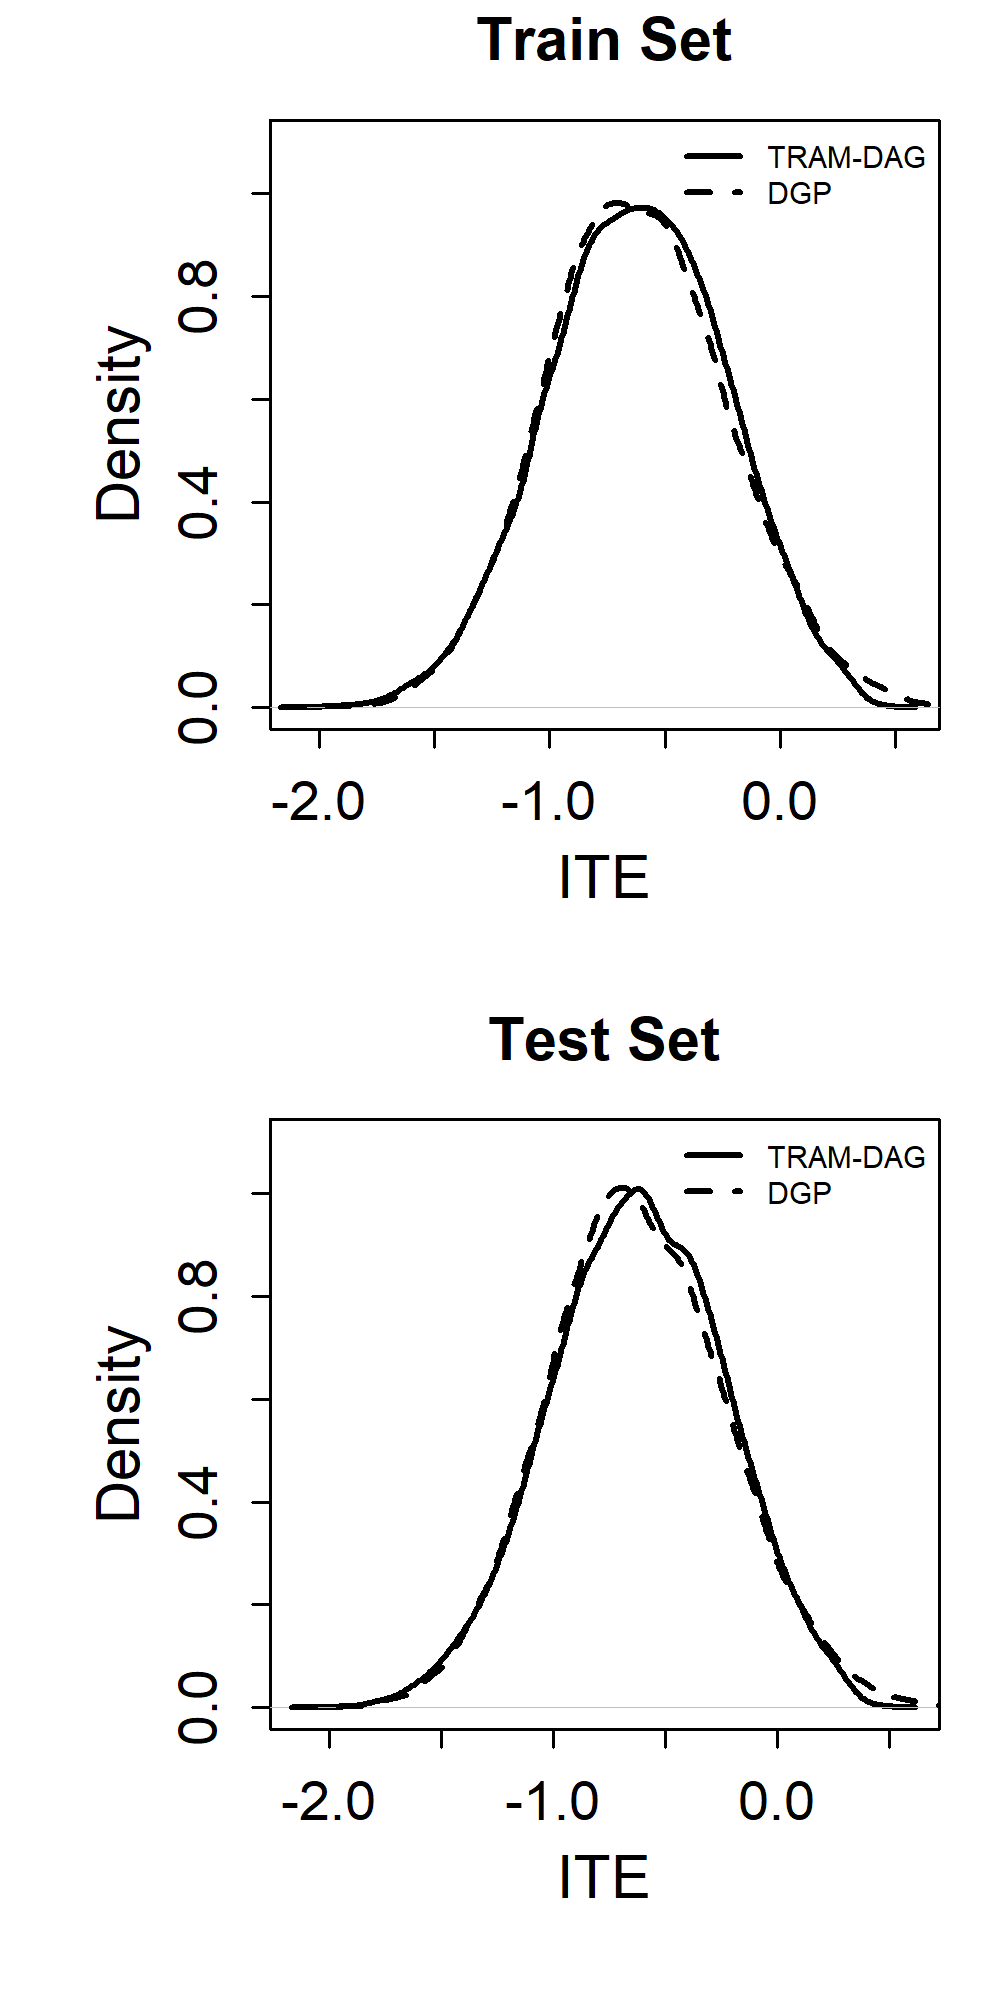
\includegraphics[width=0.33\textwidth]{img/results/rct_scenario1_ITE_densities_train_test.png}
\vspace{-17pt}
\caption{Densities of the estimated ITEs compared to the true ITEs in the training and test datasets for Scenario 4.1, which includes direct and interaction effects. Left: Observational; Right: RCT setting.}
\label{fig:scenario1_ite_densities_train_test}
\end{figure}






\begin{figure}[htbp]
\centering
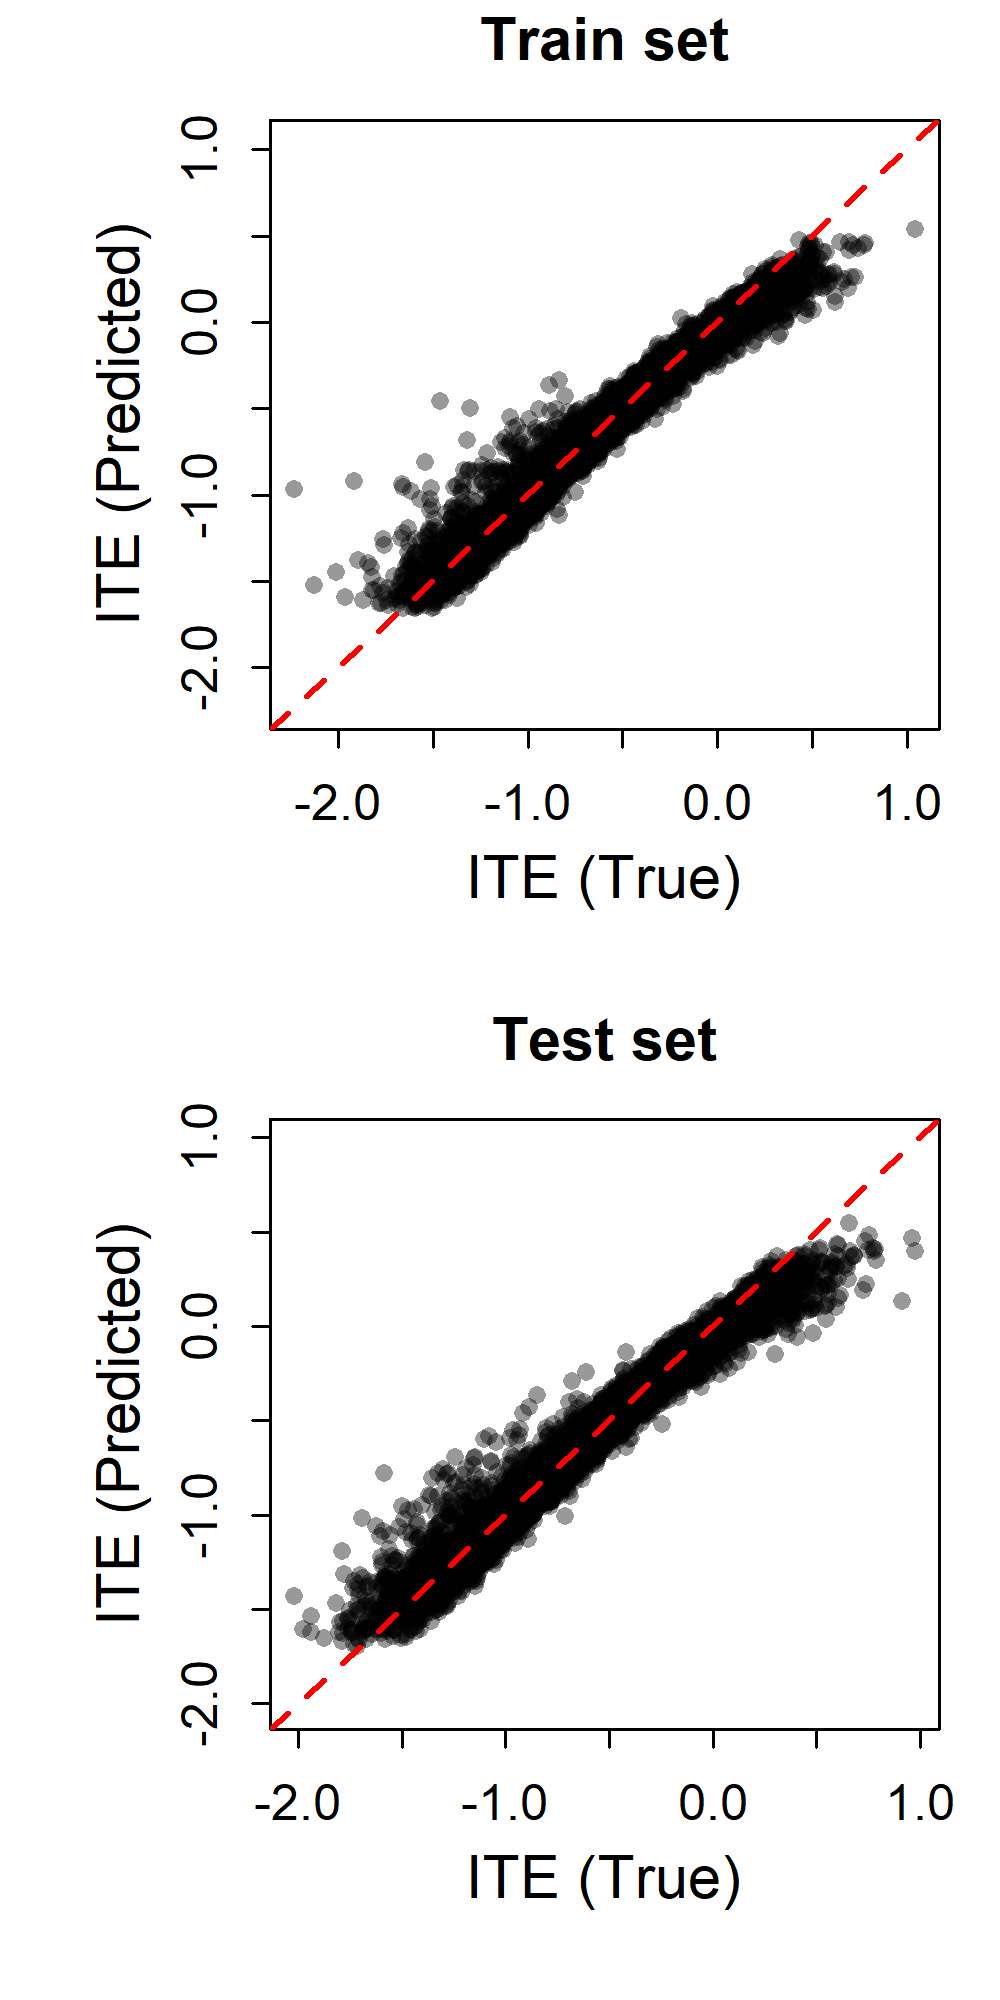
\includegraphics[width=0.33\textwidth]{img/results/observ_scenario1_ITE_scatter_train_test.png} 
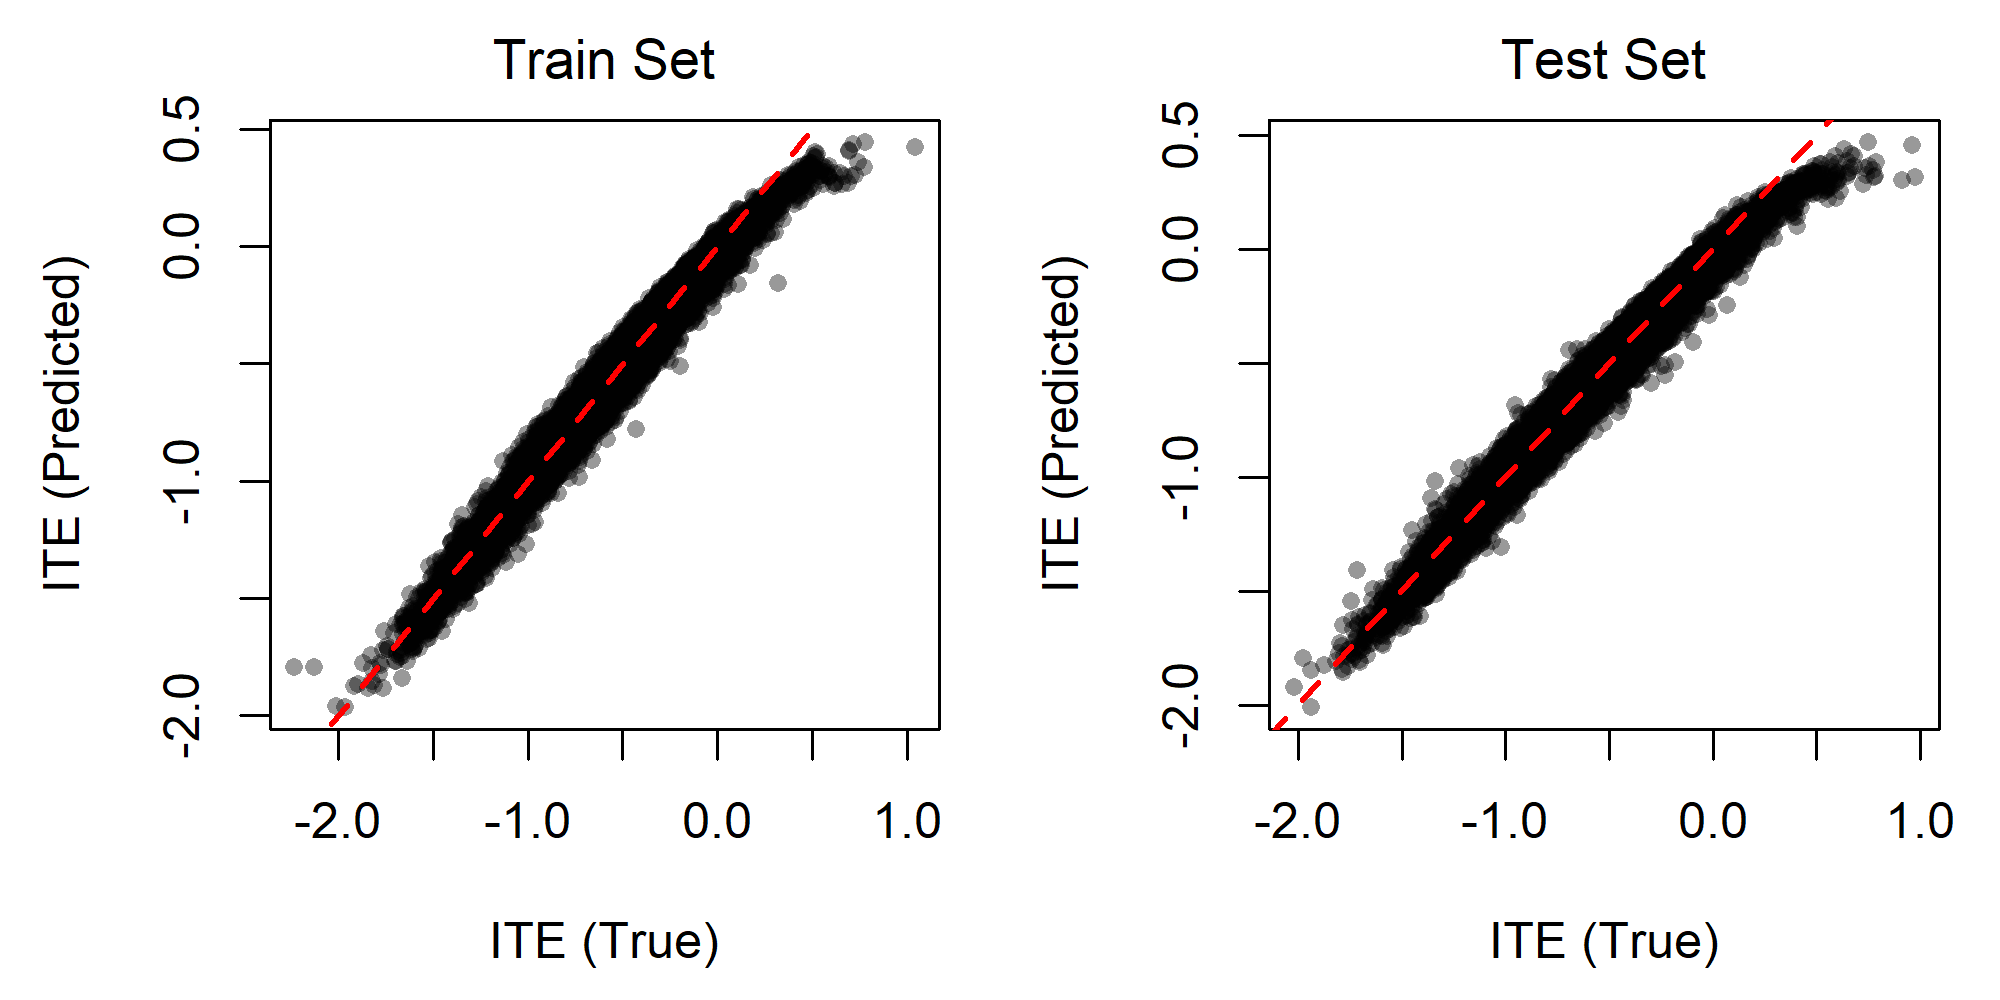
\includegraphics[width=0.33\textwidth]{img/results/rct_scenario1_ITE_scatter_train_test.png}
\vspace{-17pt}
\caption{Scatterplots of estimated ITEs vs. true ITEs in the training and test datasets for Scenario 4.1, which includes direct and interaction effects. Left: Observational; Right: RCT setting.}
\label{fig:scenario1_ite_scatter_train_test}
\end{figure}



% 
% \begin{figure}[htbp]
% \centering
% 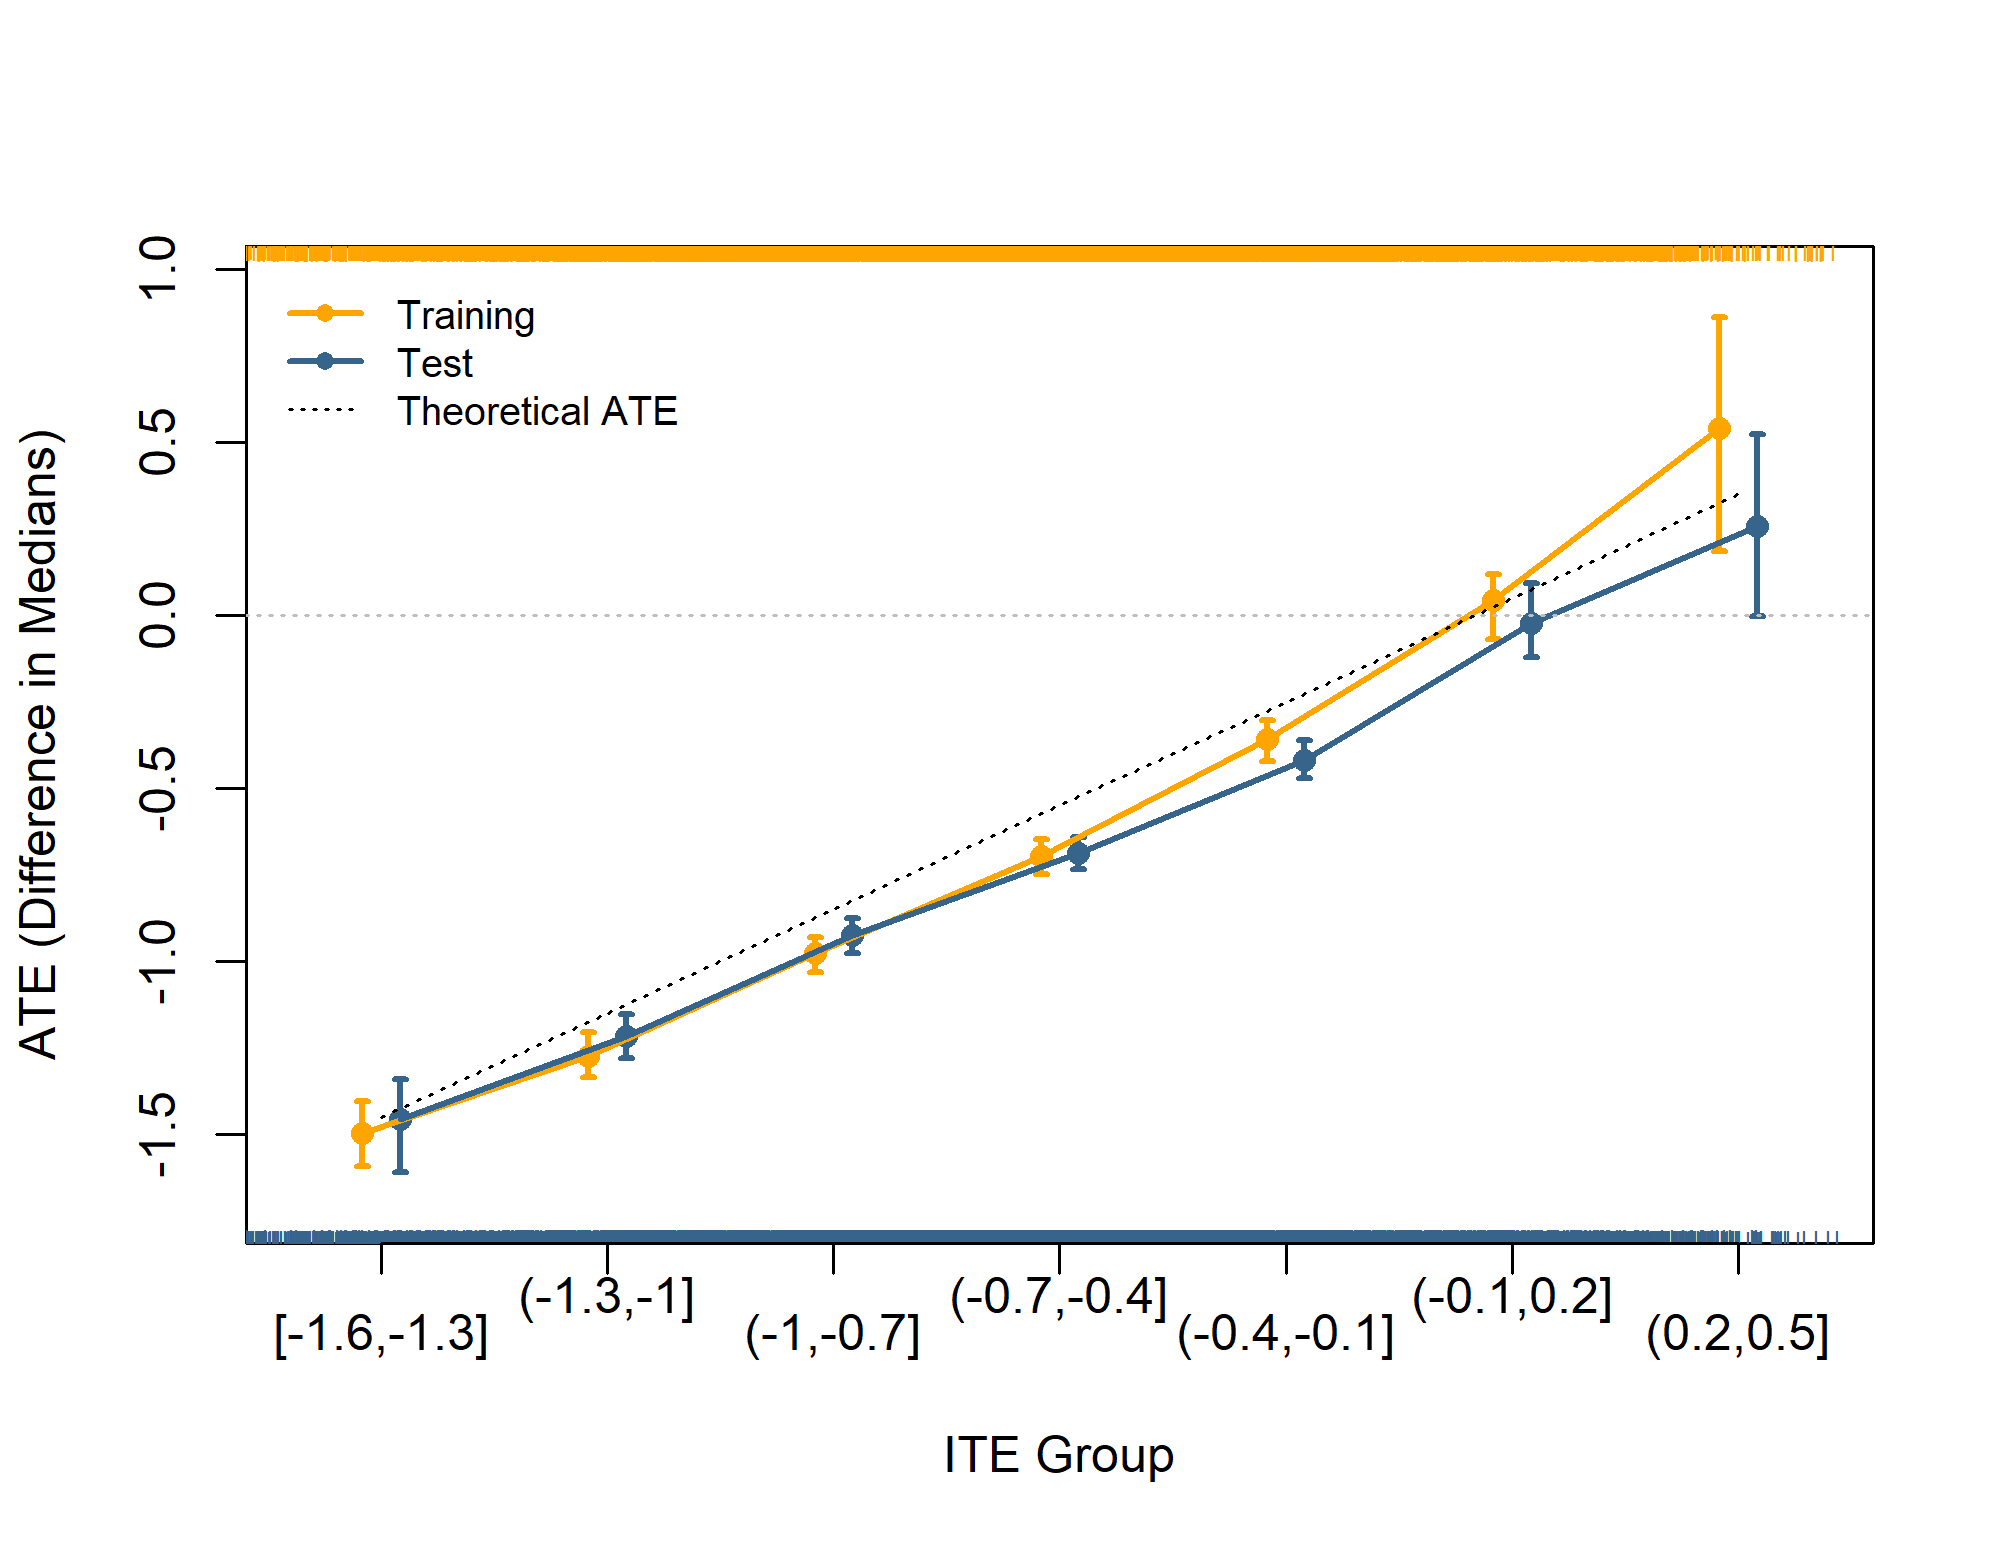
\includegraphics[width=0.45\textwidth]{img/results/observ_scenario1_ITE_ATE.png}
% 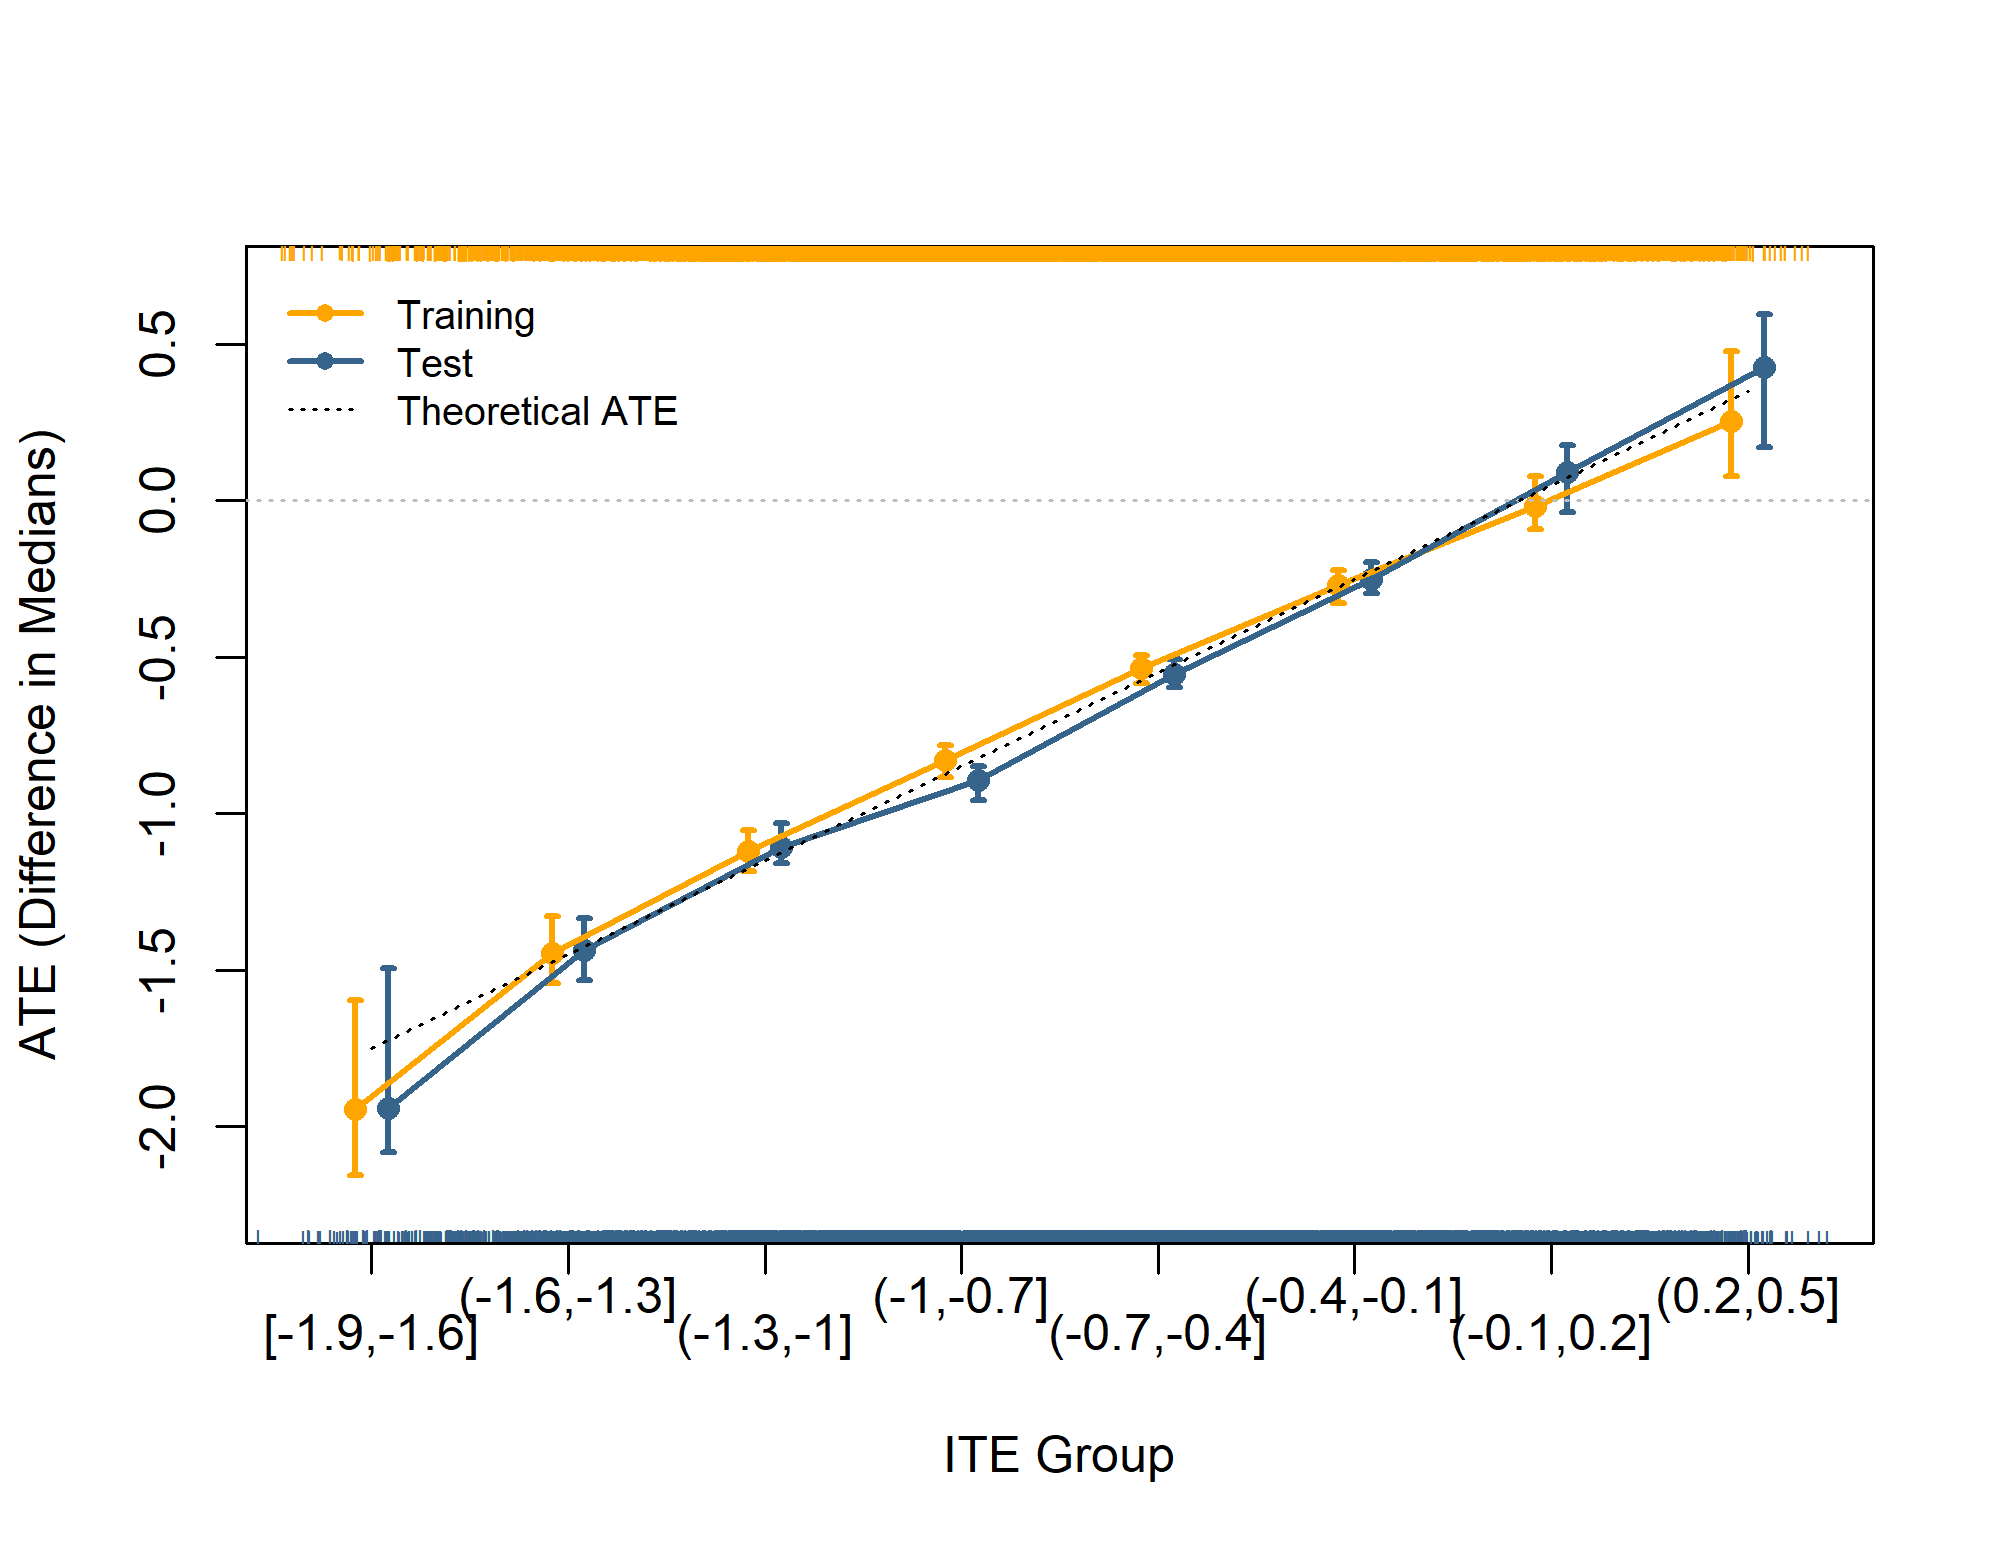
\includegraphics[width=0.45\textwidth]{img/results/rct_scenario1_ITE_ATE.png}
% \caption{ITE-ATE plots for Scenario (1), which includes direct and interaction effects. Individuals are grouped into bins based on their estimated ITEs, and within each bin, the ATE is calculated as the difference in medians of the observed outcomes under the two treatments. 95\% bootstrap confidence intervals indicate the uncertainty. Left: Observational; Right: RCT setting.}
% \label{fig:scenario1_ite_cATE}
% \end{figure}


\begin{figure}[htbp]
\centering
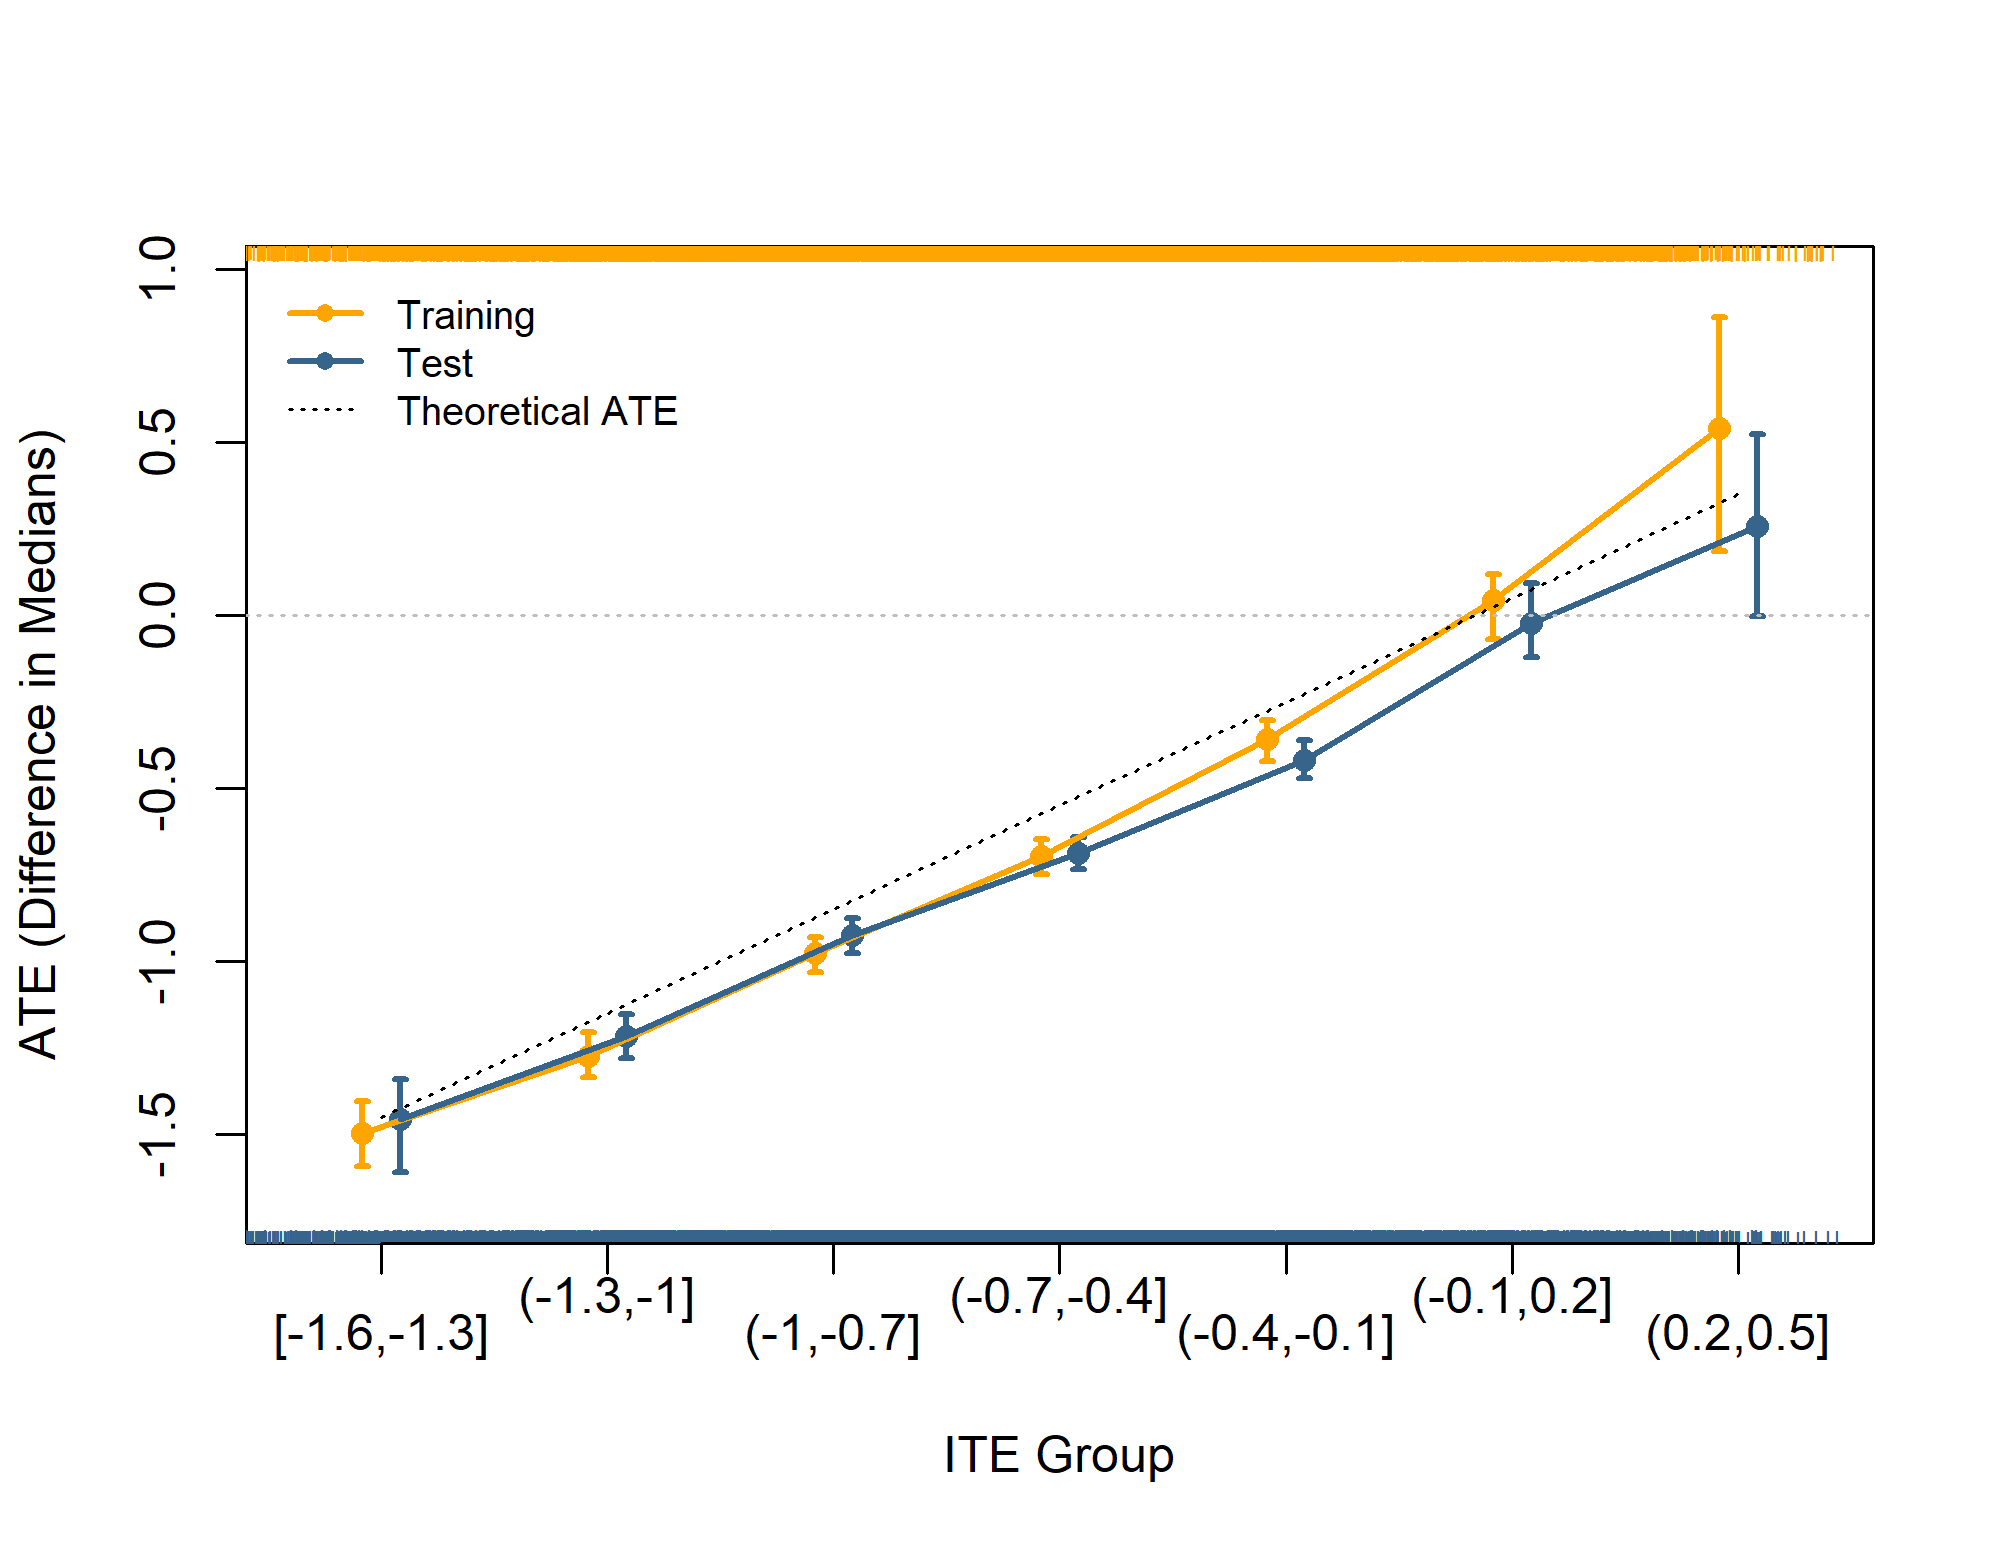
\includegraphics[width=0.8\textwidth]{img/results/observ_scenario1_ITE_ATE.png}
\vspace{-15pt}
\caption{ITE-ATE plot for Scenario 4.1 in the observational setting, which includes direct and interaction effects. Individuals are grouped into bins based on their estimated ITEs, and within each bin, the ATE is calculated as the difference in medians of the observed outcomes under the two treatments. 95\% bootstrap confidence intervals indicate the uncertainty.}
\label{fig:observ_scenario1_ite_ATE}
\end{figure}


\begin{figure}[htbp]
\centering
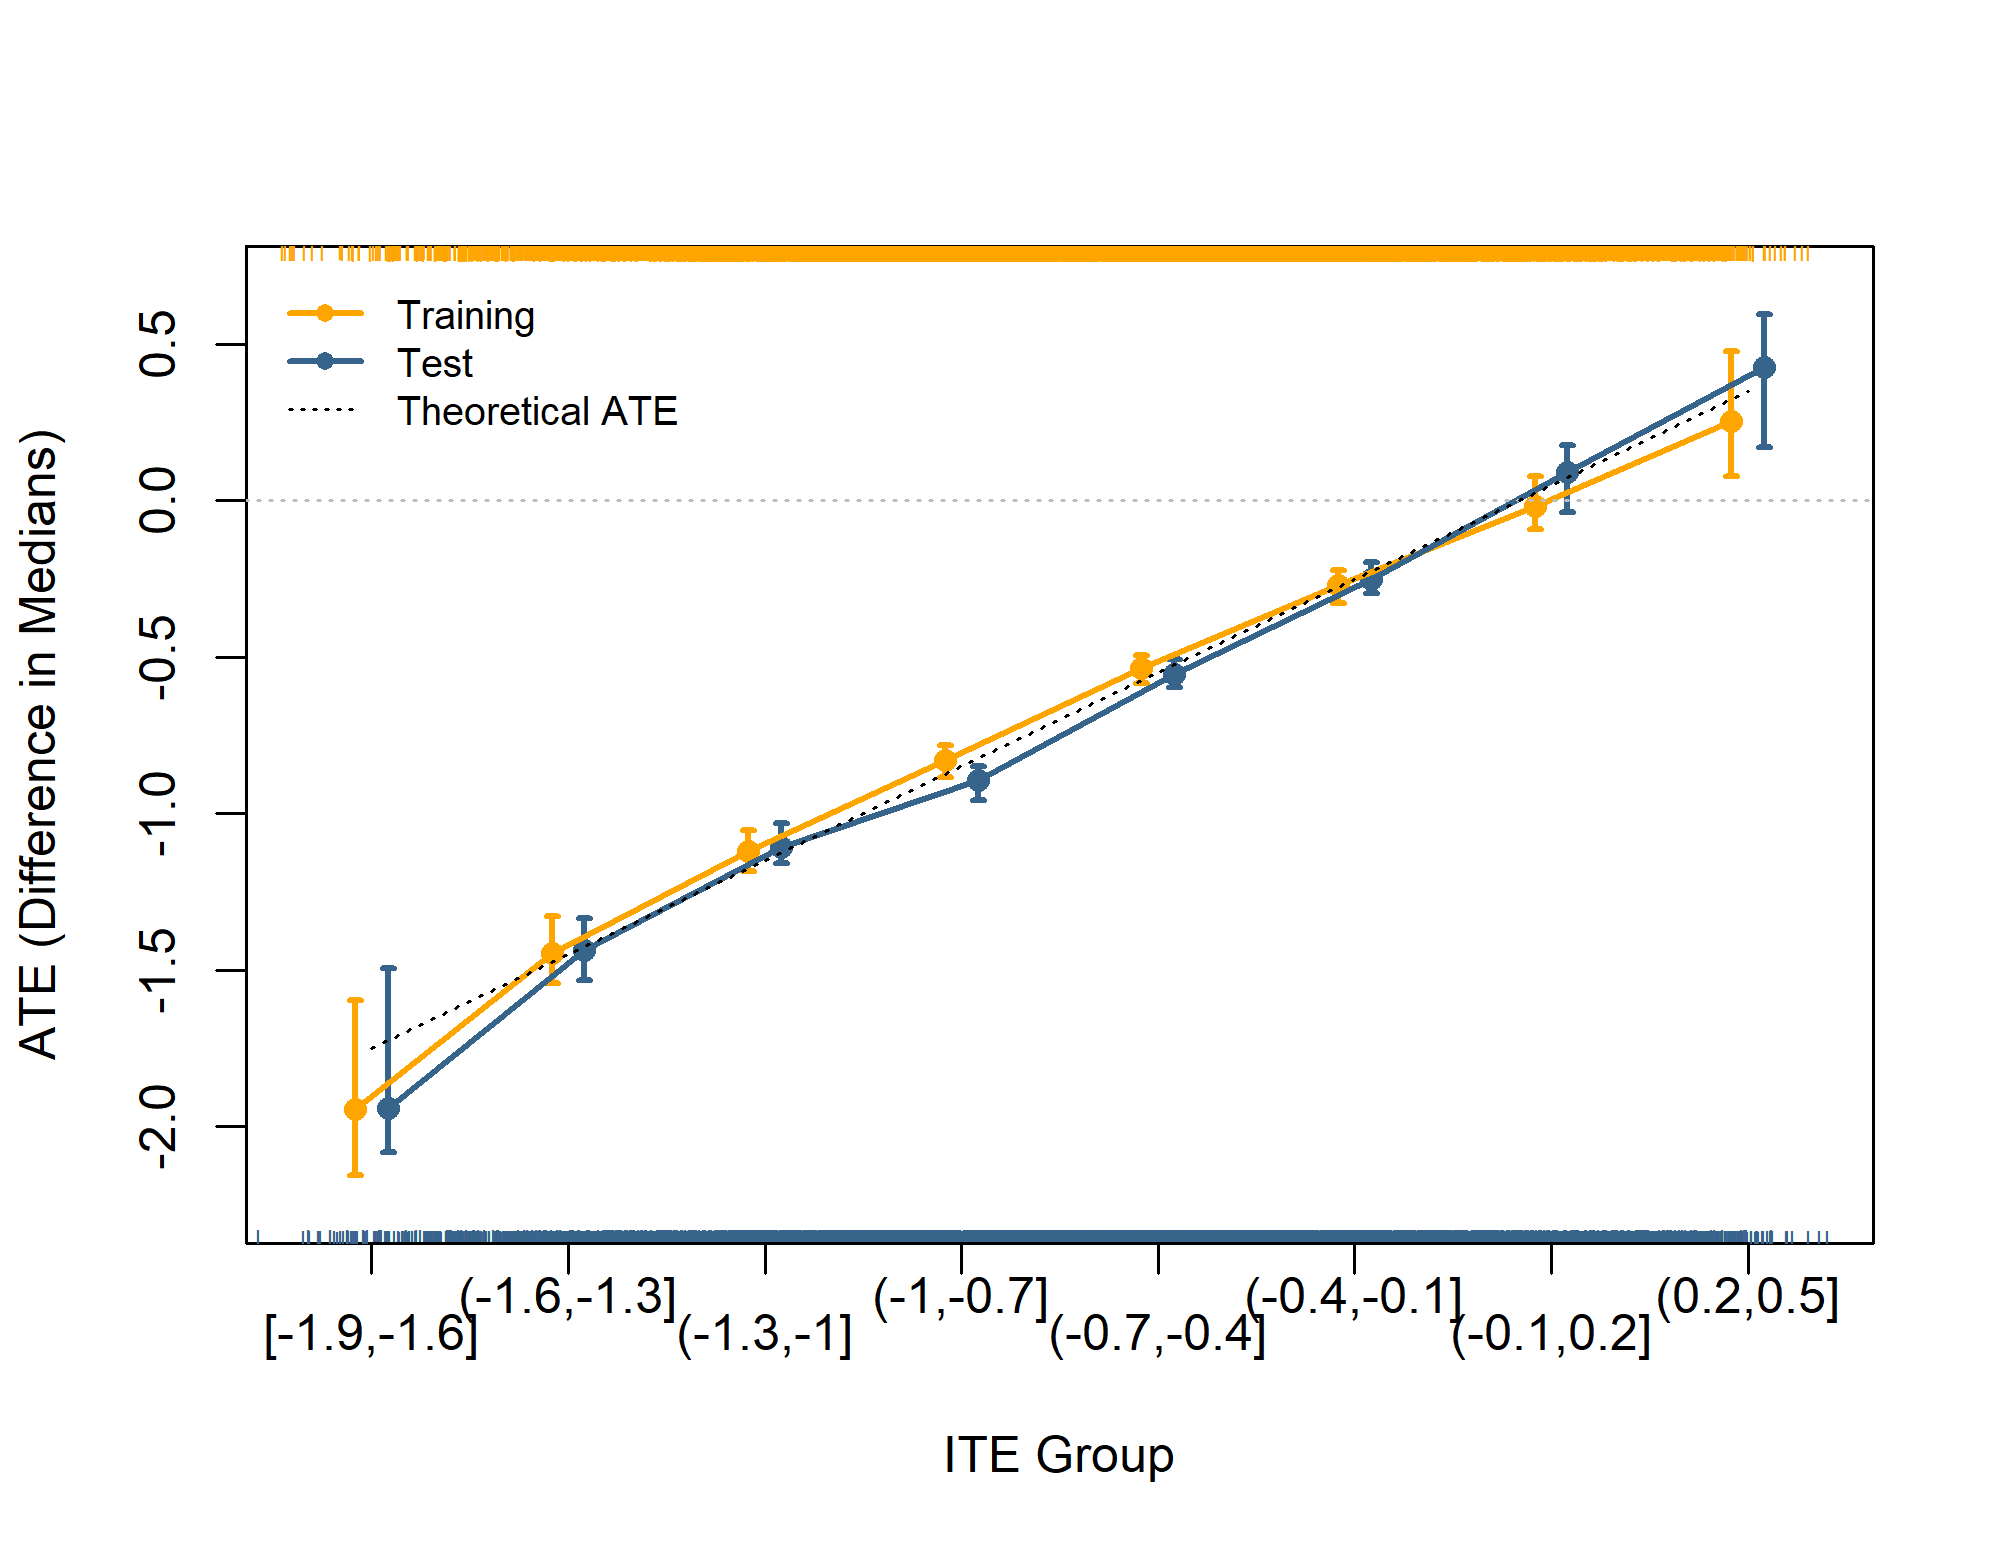
\includegraphics[width=0.8\textwidth]{img/results/rct_scenario1_ITE_ATE.png}
\vspace{-15pt}
\caption{ITE-ATE plot for Scenario 4.1 in the RCT setting, which includes direct and interaction effects. Individuals are grouped into bins based on their estimated ITEs, and within each bin, the ATE is calculated as the difference in medians of the observed outcomes under the two treatments. 95\% bootstrap confidence intervals indicate the uncertainty.}
\label{fig:rct_scenario1_ite_ATE}
\end{figure}


% enforce that starts after all floats have been displayed
\FloatBarrier


\textbf{Discussion of Scenario~4.1:} The TRAM-DAG successfully estimatet the ITEs in Scenario~4.1 where a direct effect and interaction effects were present. There was no notable difference in estimation accuracy between the observational and RCT settings. Scatterplots of estimated ITEs vs. true ITEs showed good prediction accuracy (see Figure \ref{fig:scenario1_ite_scatter_train_test}). The ATE based on the mean of the estimated ITEs closely matched the ATE derived from the true ITEs in both scenarios (see Table \ref{tab:scenario1_ate_comparison}). These results highlight TRAM-DAG's ability to compute counterfactuals for mediators and to estimate ITEs even in relatively complex DAG structures.


% start a new page
\clearpage


\subsubsection{Scenario 4.2: With direct effect, but no interaction effects} \label{sec:exp4_sc2}

\begin{figure}[H]
\centering
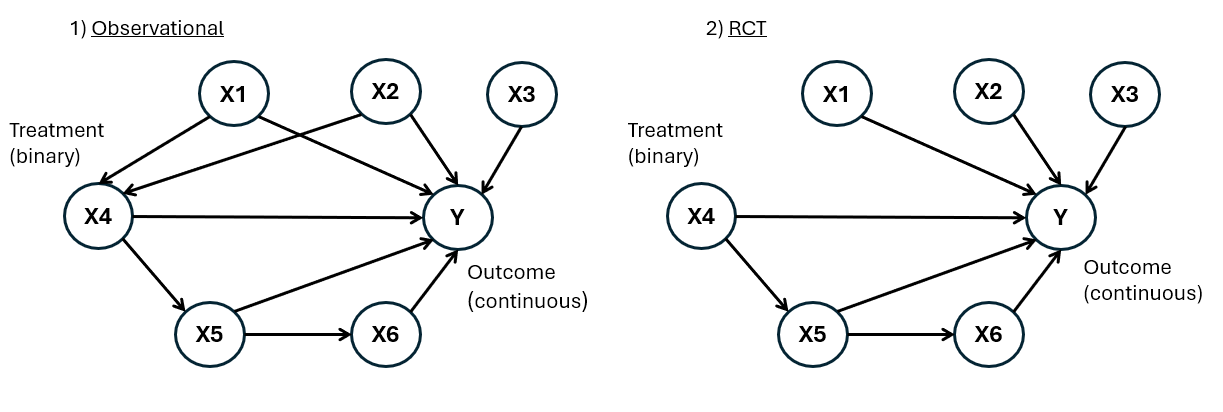
\includegraphics[width=0.85\textwidth]{img/exp4_dag_2.png}
\caption{DAGs for Scenario~4.2, which includes a direct effect of the treatment on the outcome, but no interaction effects that would induce treatment effect heterogeneity. Left: Observational; Right: RCT setting.}
\label{fig:ite_dag_observational_2}
\end{figure}

Scenario~4.2 includes a direct effect of the treatment on the outcome, while the coefficients for the interaction terms are set to zero. This results in less heterogeneity in the ITE distribution compared to Scenario~4.1 (Section~\ref{sec:exp4_sc1}), as shown in Figure~\ref{fig:scenario2_ite_distribution_dgp}. The reason for the remaining heterogeneity despite the absence of explicit interactions is discussed at the end of this section.
The observational and interventional densities generated by the fitted TRAM-DAG closely approximate the true DGP-defined distributions for all variables, as illustrated in Figures~\ref{fig:scenario2_sampling_distributions_vertical} and~\ref{fig:scenario2_outcome_distributions}. However, there is a notable difference in variance between the estimated and true ITE distributions, visible in Figures~\ref{fig:scenario2_ite_densities_train_test} and~\ref{fig:scenario2_ite_scatter_train_test}. The ITE-ATE plots in Figures~\ref{fig:observ_scenario2_ite_ATE} and \ref{fig:rct_scenario2_ite_ATE} are less informative than those in Scenario~1, which is as expected given the reduced heterogeneity. Table~\ref{tab:scenario2_ate_comparison} presents the ATE measures for Scenario~2. In the test set of the RCT setting, the ATE based on the true ITEs was -0.633, while the ATE based on the estimated ITEs was -0.586.

In the RCT setting (training set), the difference in means of the outcomes between the two treatment groups was 
$-0.569$, with a 95\% Wald confidence interval from 
$-0.588$ to 
$-0.550$. Note that the ATE in terms of difference in means cannot be directly compared to the ATE based on difference in medians.



\begin{table}[htbp]
\centering
\small
\caption{Scenario~4.2, including a direct treatment effect but no interaction effects: Comparison of ATE measures across train and test sets for the observational and RCT setting. $\text{Y}_\text{observed}^{(\text{Tr})}$ denotes the observed outcome under the treatment ($\text{Tr}$) actually received. Estimates based on these observed outcomes (means and medians) are provided only for the RCT setting, as the observational setting is confounded. The true ITEs ($\text{ITE}_\text{true}$) were calculated for each individual based on the data-generating process. In contrast, the estimated ITEs ($\text{ITE}_\text{estimated}$) were obtained from the TRAM-DAG trained on observed data. The estimated ATE from $\text{mean}(\text{ITE}_\text{estimated})$ can be directly compared to the true $\text{mean}(\text{ITE}_\text{true})$, whereas comparisons to empirical ATEs from observed outcome differences should be interpreted with caution. All ITEs were computed as quantile treatment effects (QTEs) based on the median of the potential outcome distributions, as defined in Equation~\ref{eq:qte}.}
\label{tab:scenario2_ate_comparison}
\begin{tabular}{l c c c c}
\toprule
\textbf{Measure} & \multicolumn{2}{c}{\textbf{Observational}} & \multicolumn{2}{c}{\textbf{RCT}} \\
\cmidrule(lr){2-3} \cmidrule(lr){4-5}
 & \textbf{Train} & \textbf{Test} & \textbf{Train} & \textbf{Test} \\
\midrule
ATE as $\text{mean}(\text{Y}_\text{observed}^{(1)}) - \text{mean}(\text{Y}_\text{observed}^{(0)})$ 
& NA & NA 
& -0.569 
& -0.572 \\

ATE as $\text{median}(\text{Y}_\text{observed}^{(1)}) - \text{median}(\text{Y}_\text{observed}^{(0)})$  
& NA & NA 
& -0.629 
& -0.639 \\

ATE as mean(ITE$_\text{true}$)  
& -0.633 
& -0.633 
& -0.633 
& -0.633 \\

ATE as mean(ITE$_\text{estimated}$) 
& -0.645 
& -0.644 
& -0.587 
& -0.586 \\
\bottomrule
\end{tabular}
\end{table}

% 
% \begin{table}[htbp]
% \centering
% \small
% \caption{Scenario (2), including a direct treatment but no interaction effects: Comparison of ATE measures across train and test sets for the observational and RCT setting.}
% \label{tab:scenario2_ate_comparison_old}
% \begin{tabular}{l c c c c}
% \toprule
% \textbf{Measure} & \multicolumn{2}{c}{\textbf{Observational}} & \multicolumn{2}{c}{\textbf{RCT}} \\
% \cmidrule(lr){2-3} \cmidrule(lr){4-5}
%  & \textbf{Train} & \textbf{Test} & \textbf{Train} & \textbf{Test} \\
% \midrule
% ATE as $\text{mean}(\text{Y}_\text{observed}^{(1)}) - \text{mean}(\text{Y}_\text{observed}^{(0)})$ & NA & NA & round(rct_scenario2$dev_ATE_observed_Y_mean_diff, 3) & round(rct_scenario2$val_ATE_observed_Y_mean_diff, 3) \\
% ATE as $\text{median}(\text{Y}_\text{observed}^{(1)}) - \text{median}(\text{Y}_\text{observed}^{(0)})$  & NA & NA & round(rct_scenario2$dev_ATE_observed_Y_median_diff, 3) & round(rct_scenario2$val_ATE_observed_Y_median_diff, 3) \\
% ATE as mean(ITE$_\text{true}$)  & round(observ_scenario2$dev_ITE_median_average, 3) & round(observ_scenario2$val_ITE_median_average, 3) & round(rct_scenario2$dev_ITE_median_average, 3) & round(rct_scenario2$val_ITE_median_average, 3) \\
% ATE as mean(ITE$_\text{estimated}$) & round(observ_scenario2$dev_ITE_median_pred_average, 3) & round(observ_scenario2$val_ITE_median_pred_average, 3) & round(rct_scenario2$dev_ITE_median_pred_average, 3) & round(rct_scenario2$val_ITE_median_pred_average, 3) \\
% \bottomrule
% \end{tabular}
% \end{table}



\begin{figure}[htbp]
\centering
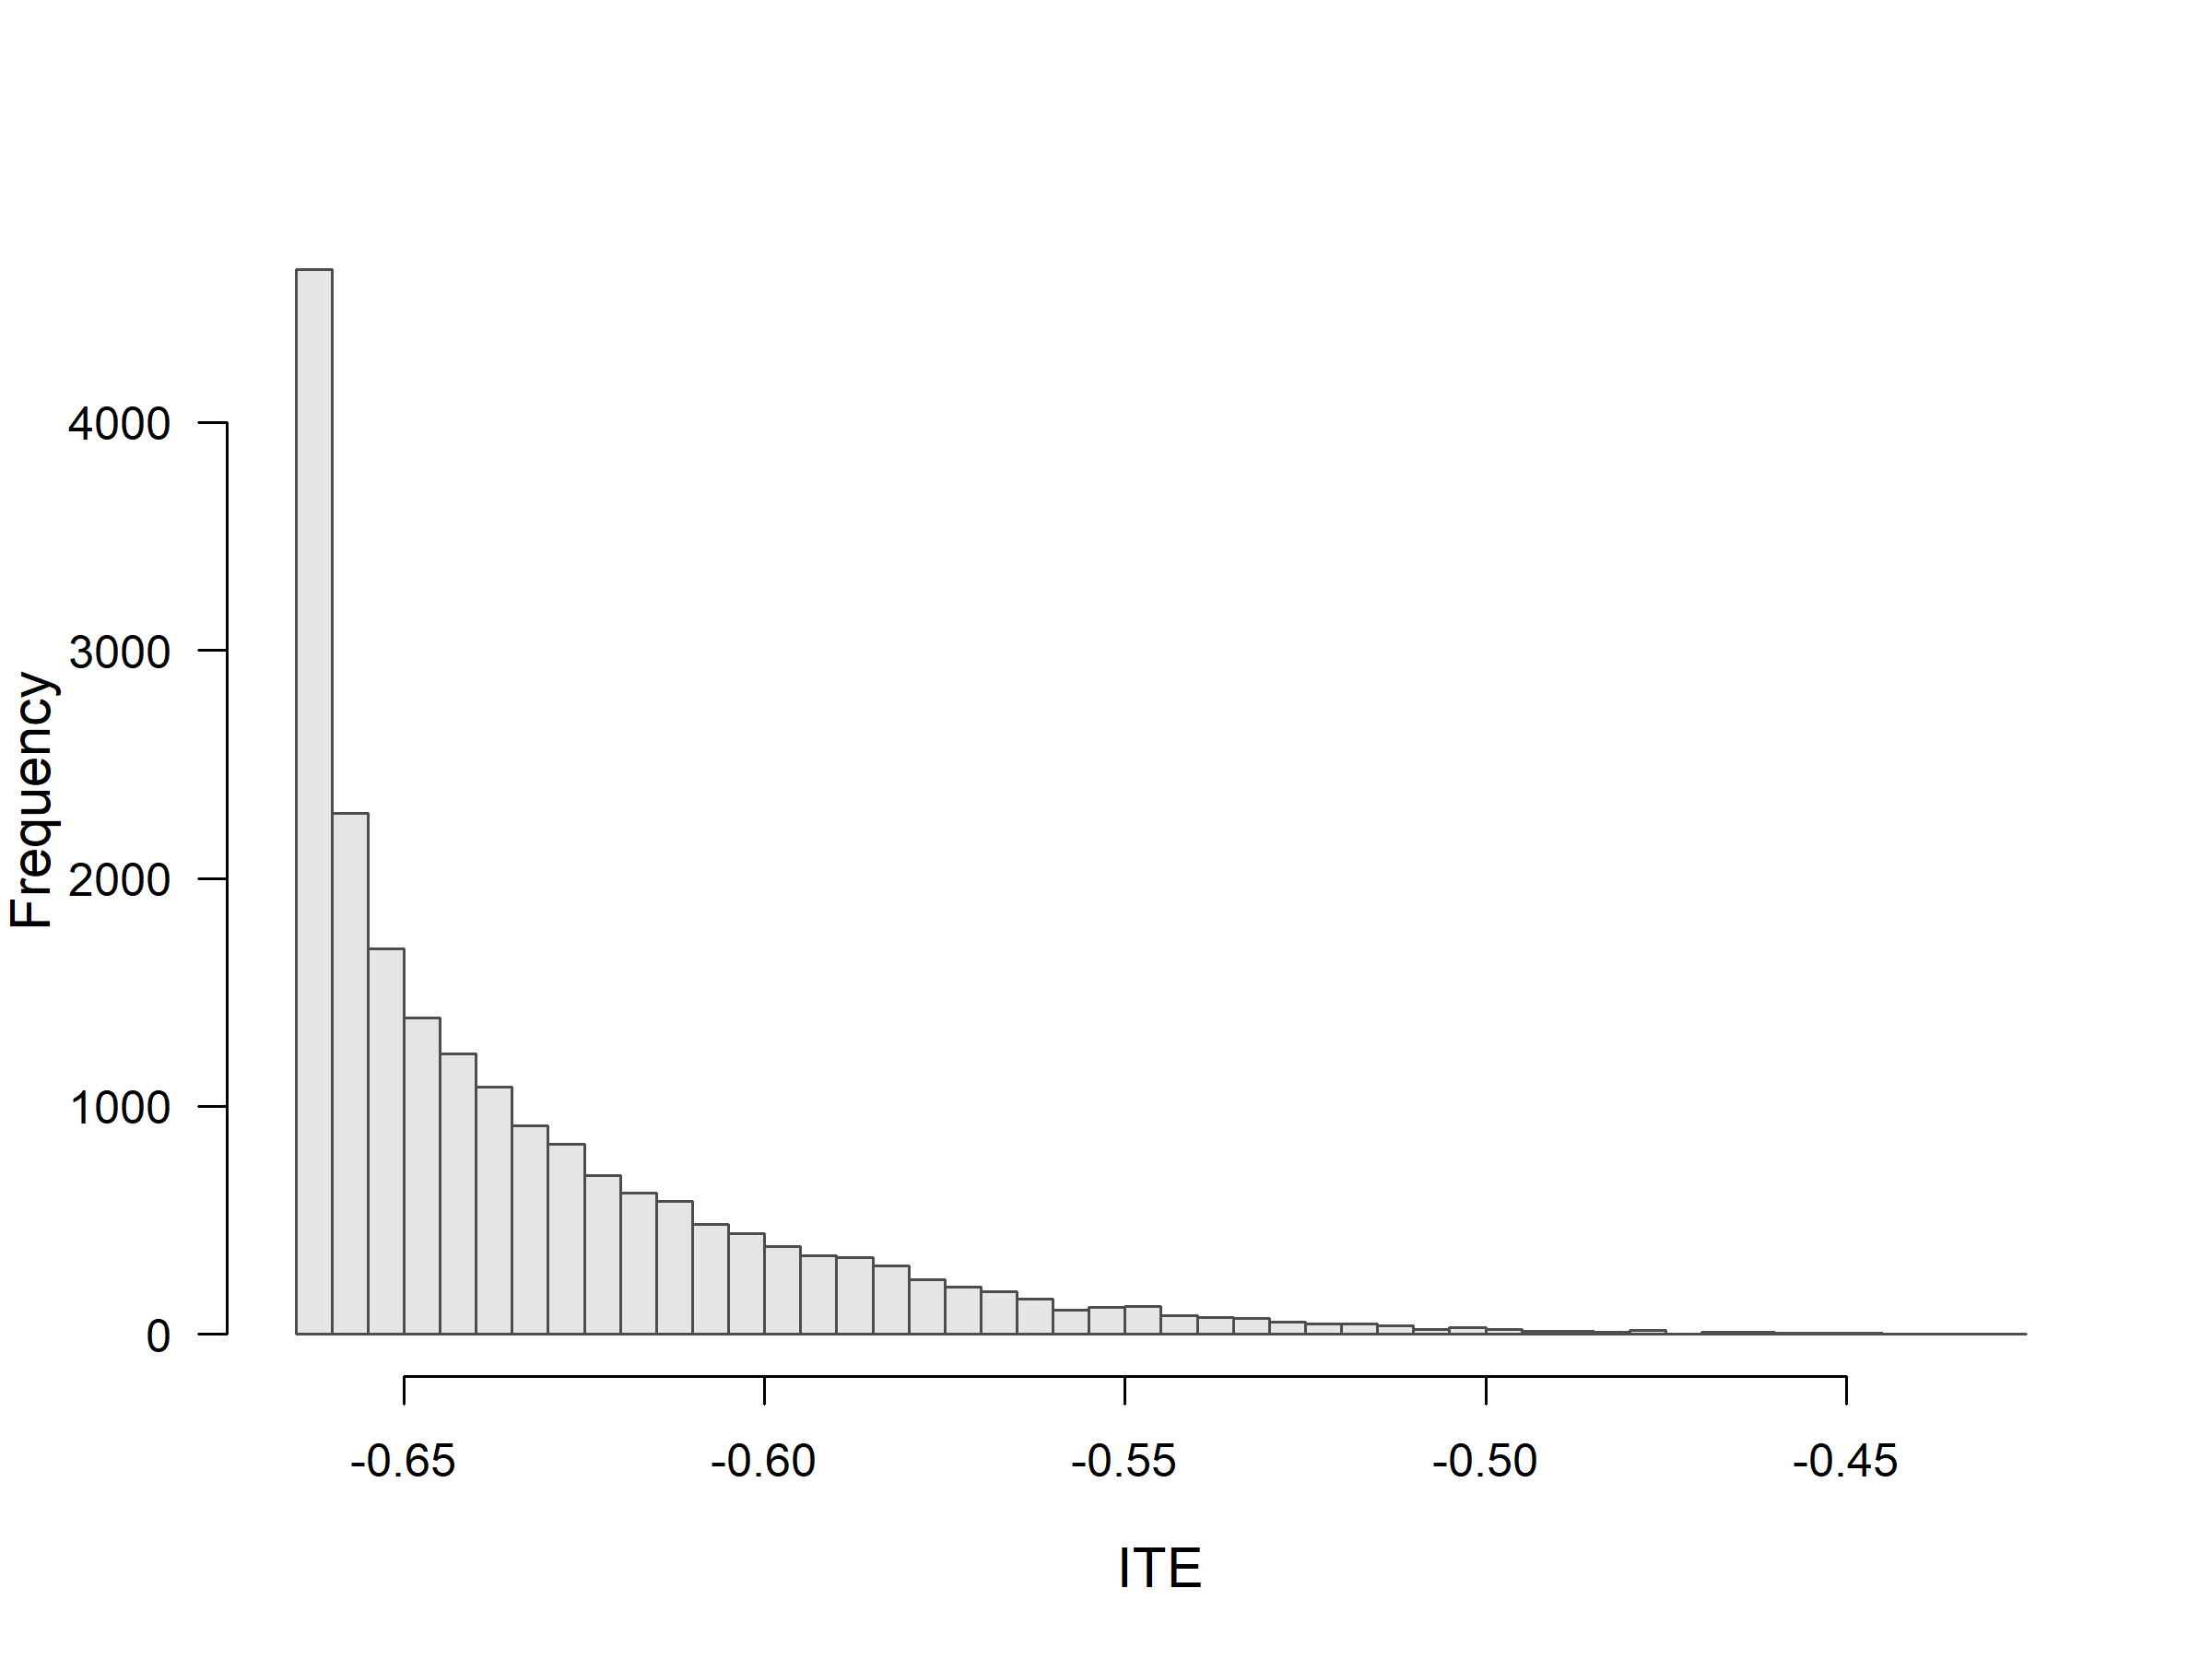
\includegraphics[width=0.7\textwidth]{img/results/observ_scenario2_ite_distribution_dgp.png}
\caption{True ITE distribution resulting from the DGP for Scenario~4.2, which includes a direct treatment effect but no interaction effects. The true ITEs are identical in the observational and RCT settings, as they depend only on the potential outcomes under both treatment allocations.}
\label{fig:scenario2_ite_distribution_dgp}
\end{figure}


\begin{figure}[htbp]
\centering
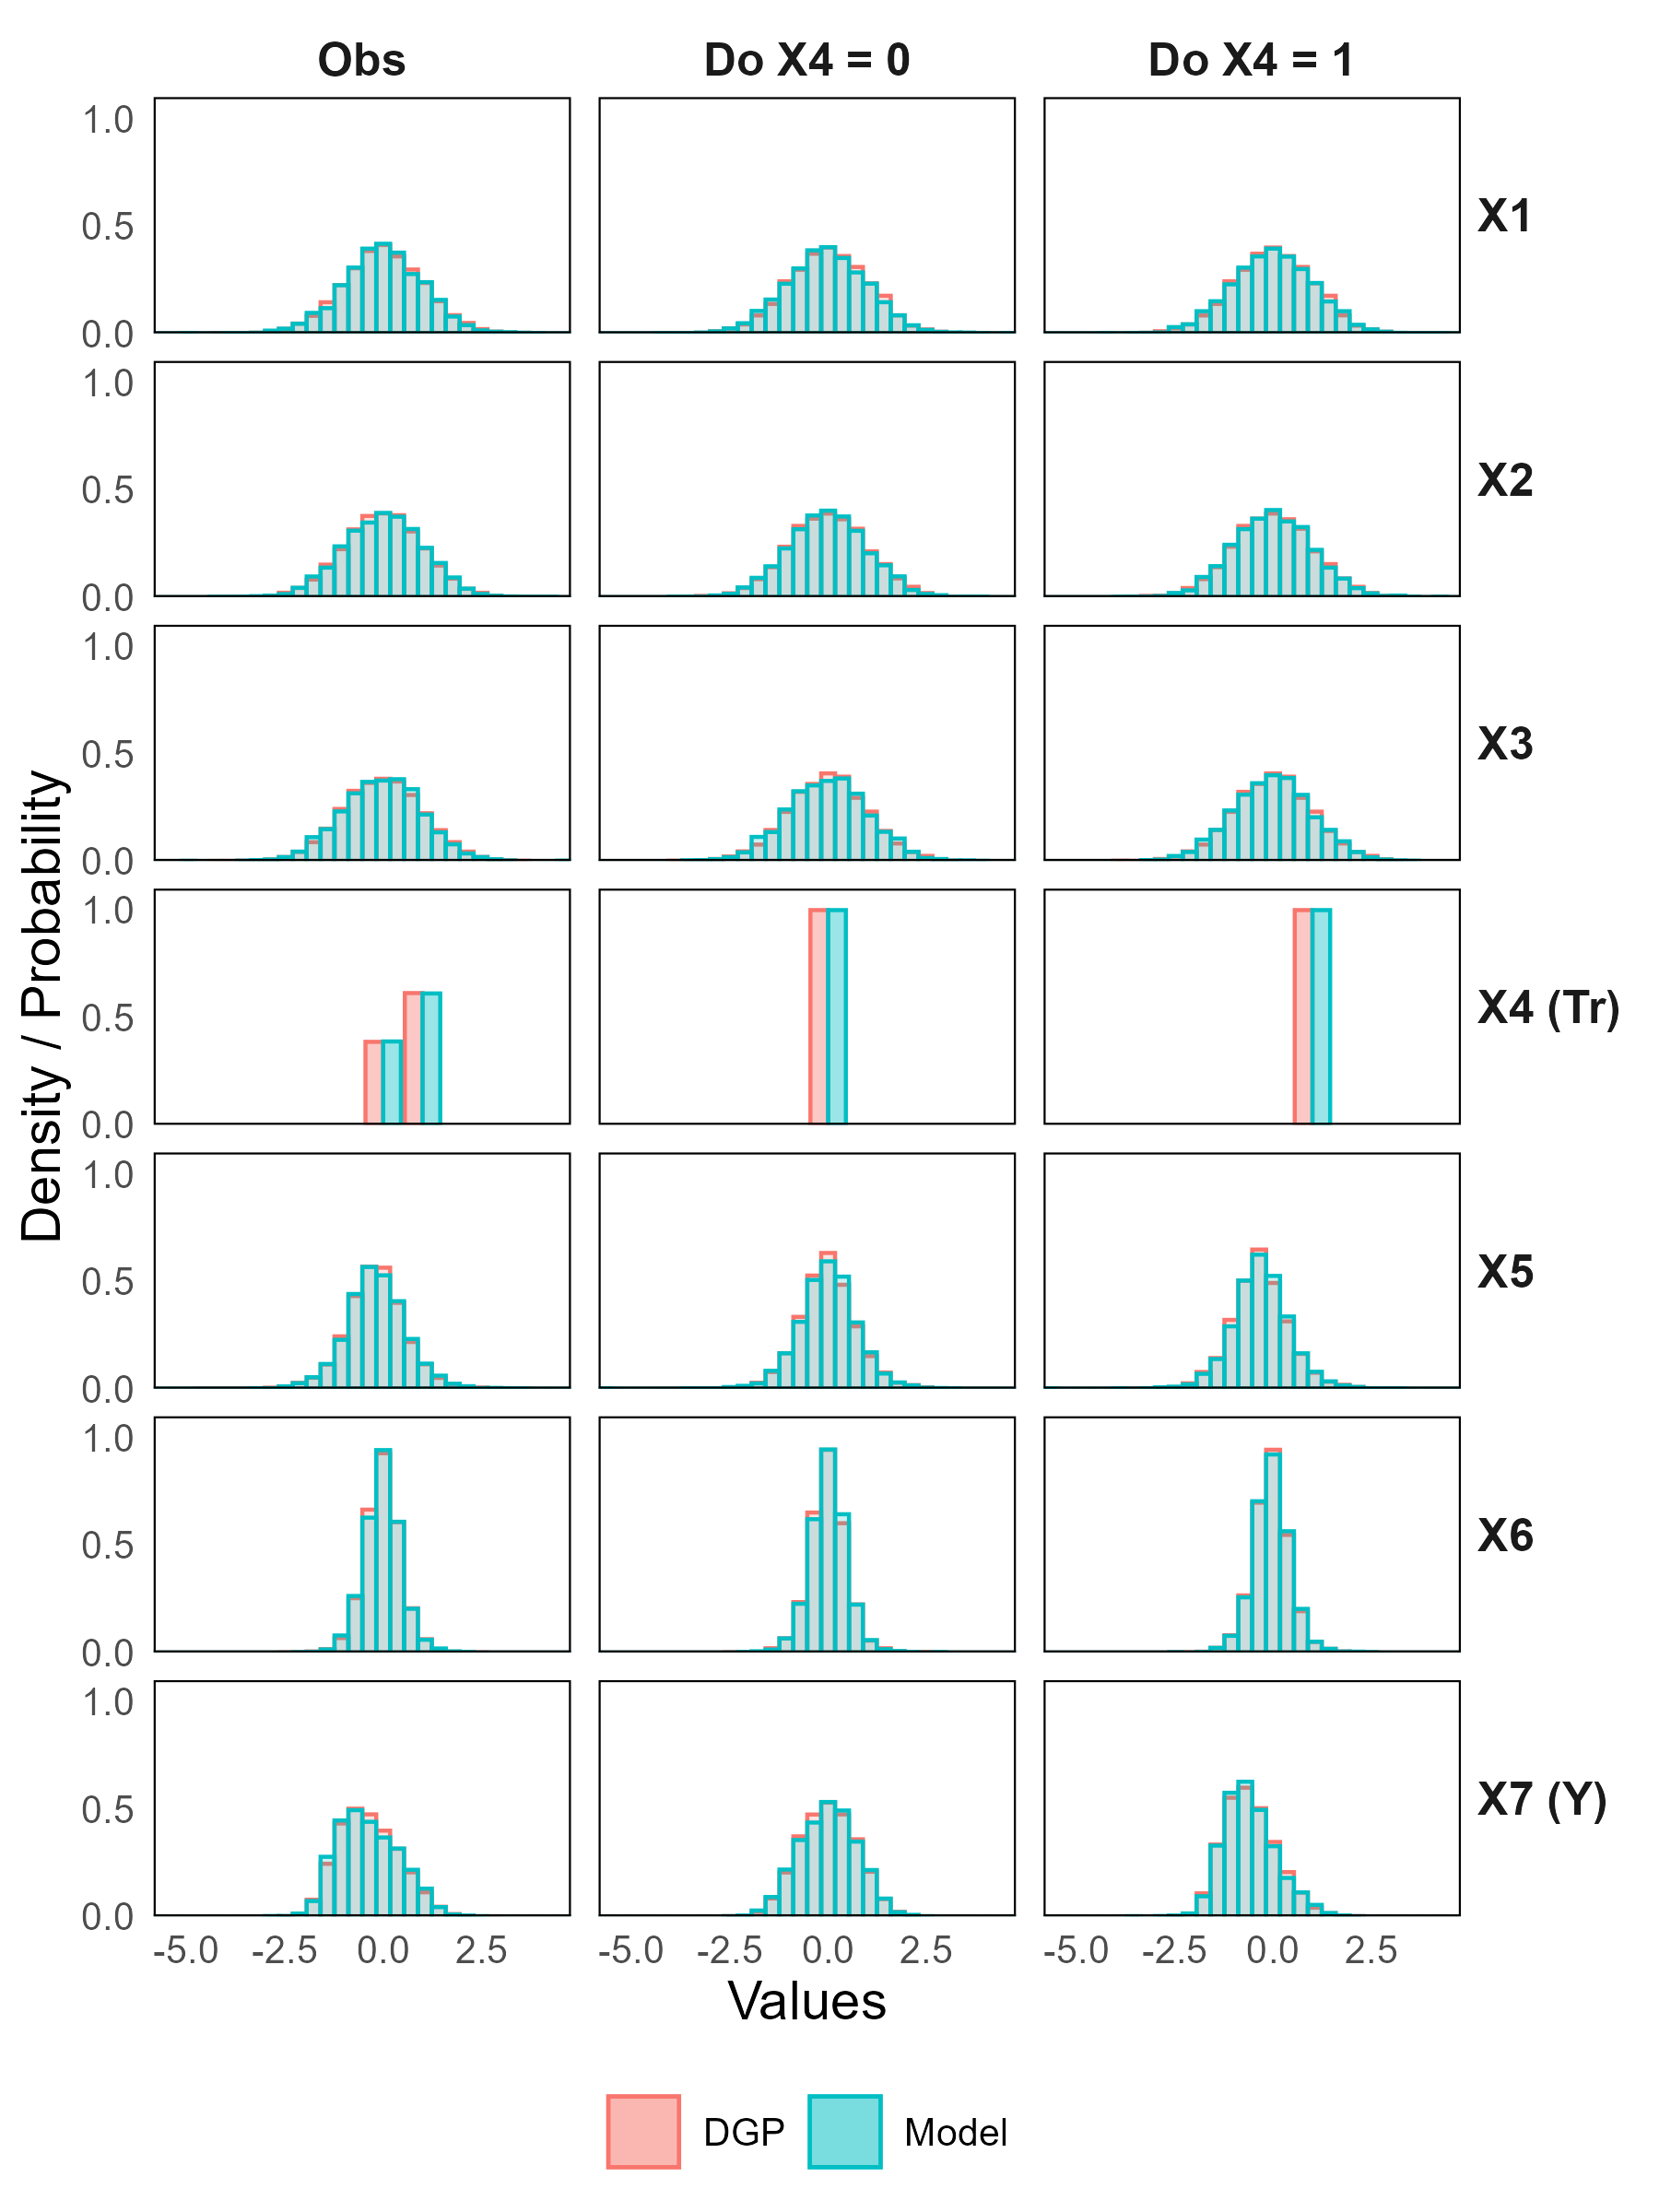
\includegraphics[width=0.45\textwidth]{img/results/observ_scenario2_sampling_distributions_vertical.png}
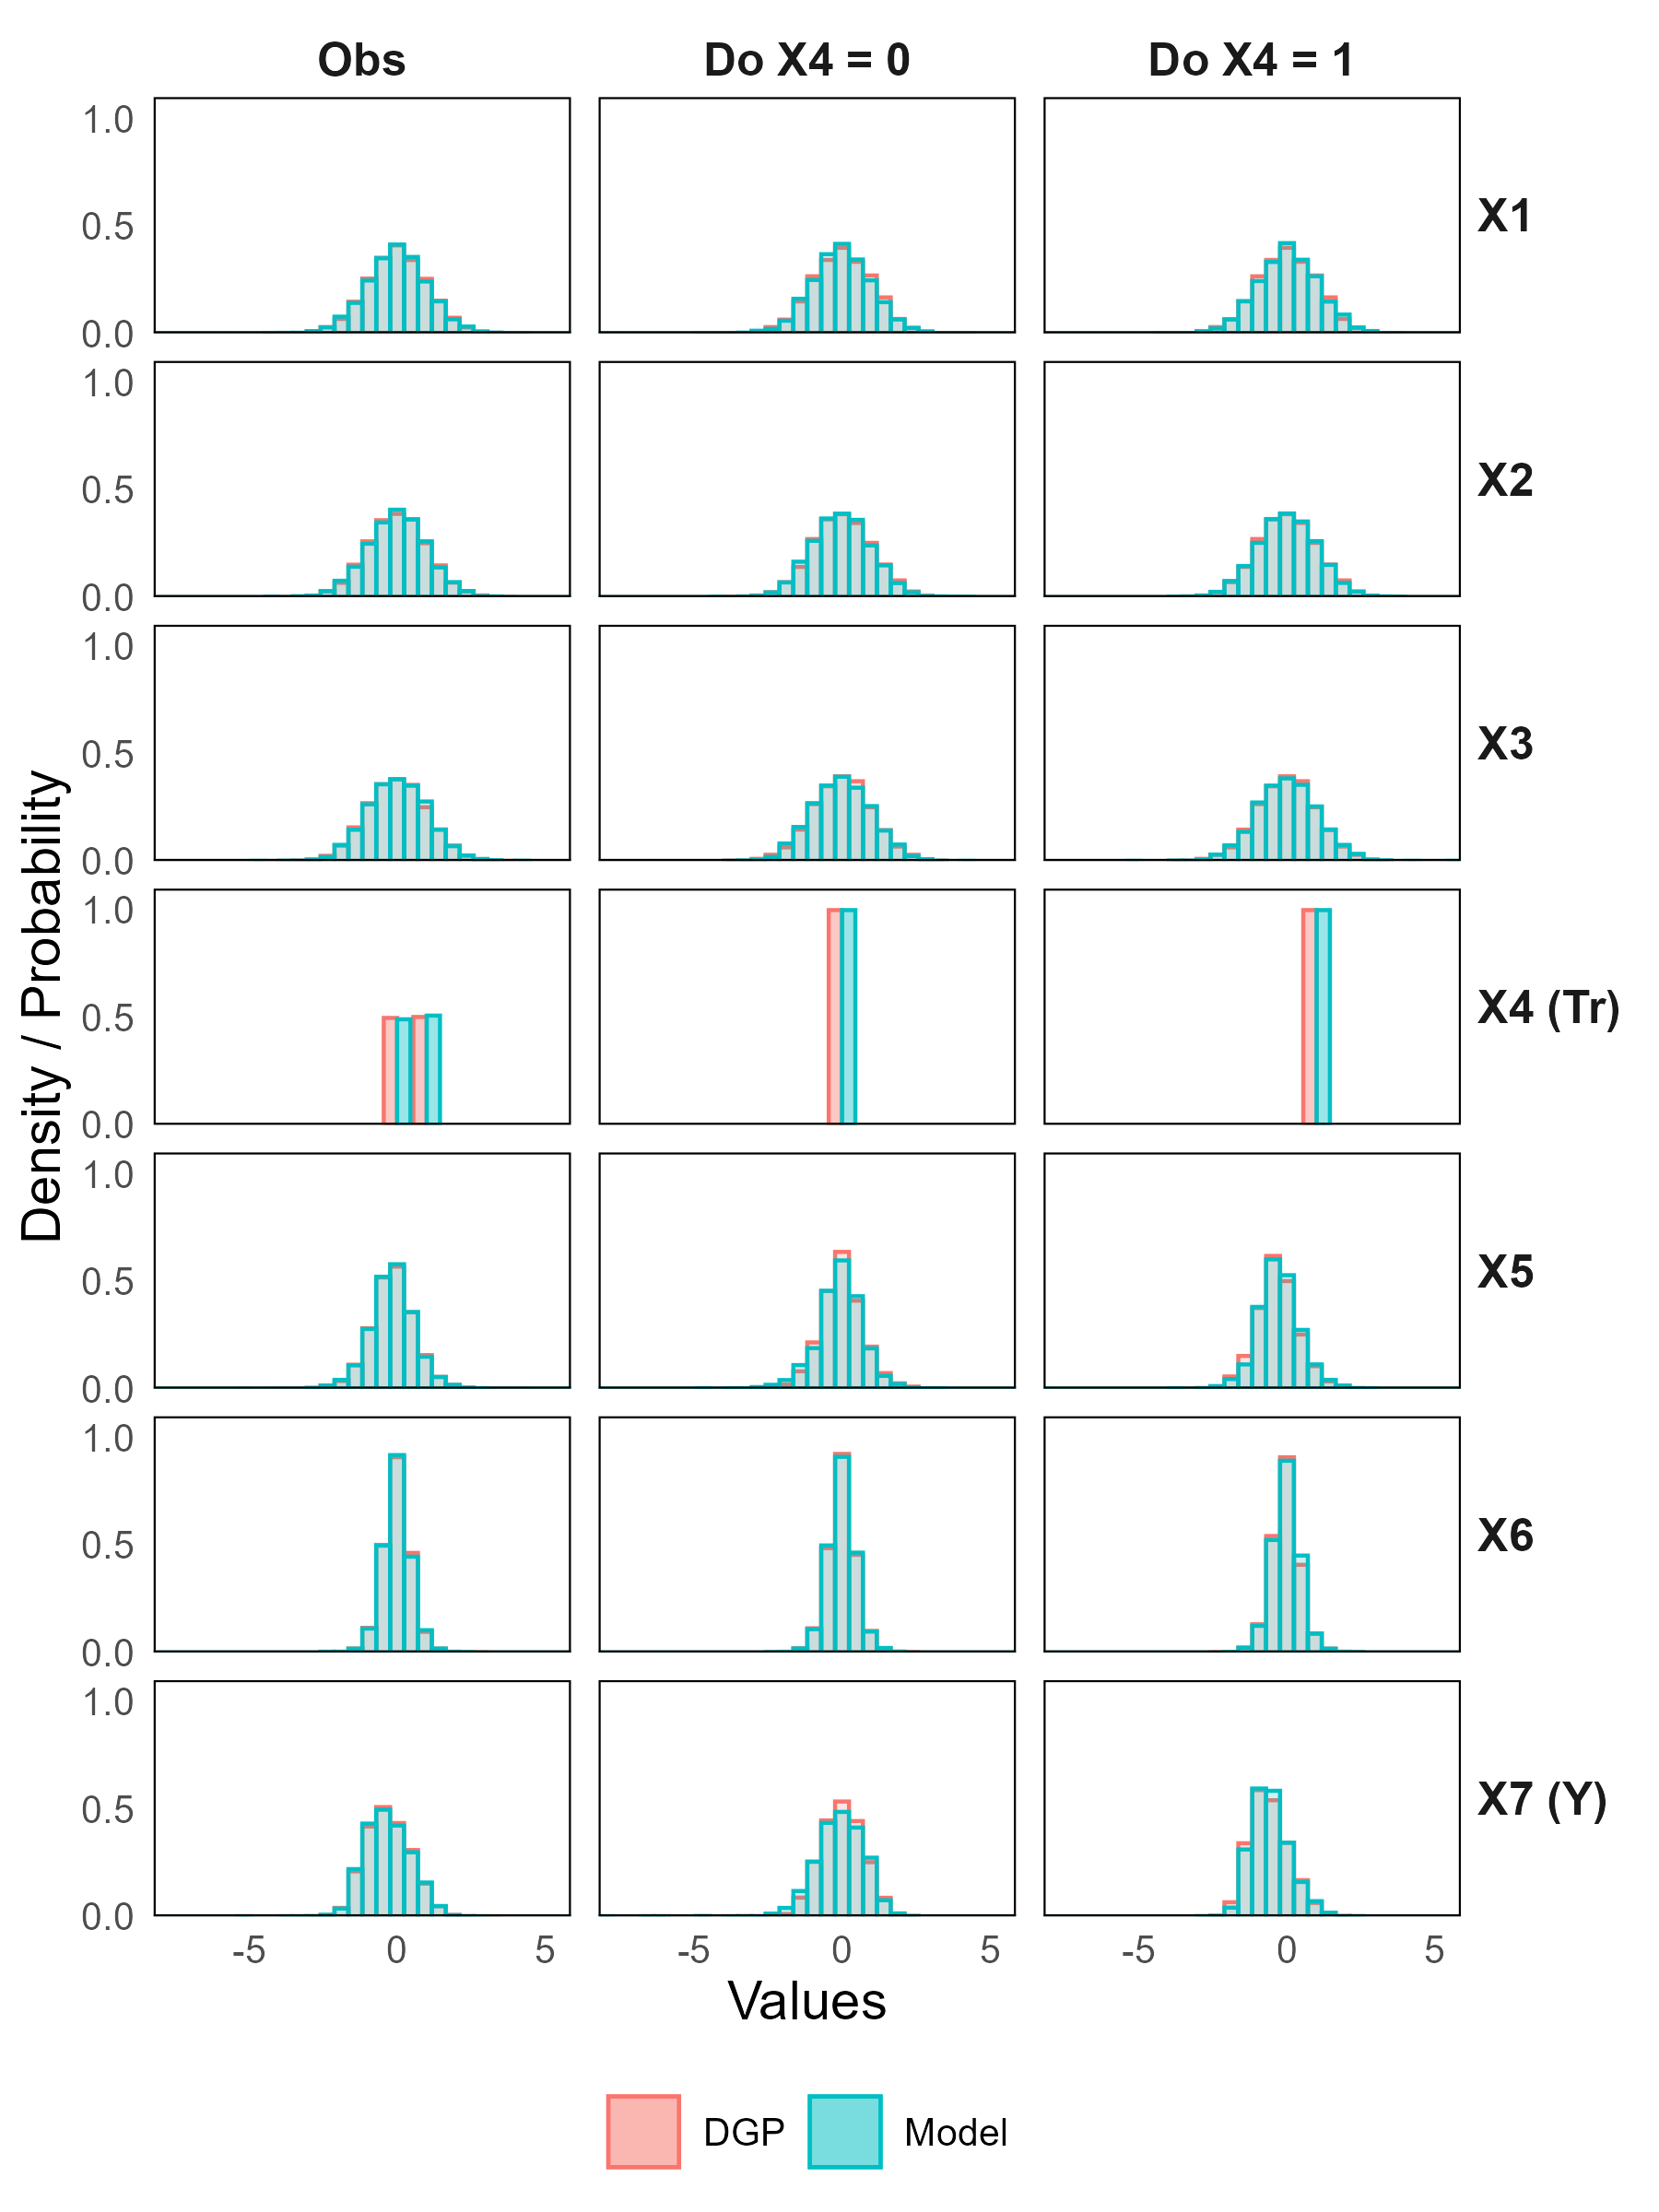
\includegraphics[width=0.45\textwidth]{img/results/rct_scenario2_sampling_distributions_vertical.png}
\caption{Marginal distributions of variables from the DGP and from samples generated by the fitted TRAM-DAG for Scenario~4.2, which includes a direct treatment effect but no interaction effects. The distributions are shown as observed (Obs), under control intervention do($X_4 = 0$), and under treatment intervention do($X_4 = 1$). Left: Observational; Right: RCT setting.}
\label{fig:scenario2_sampling_distributions_vertical}
\end{figure}


\begin{figure}[htbp]
\centering
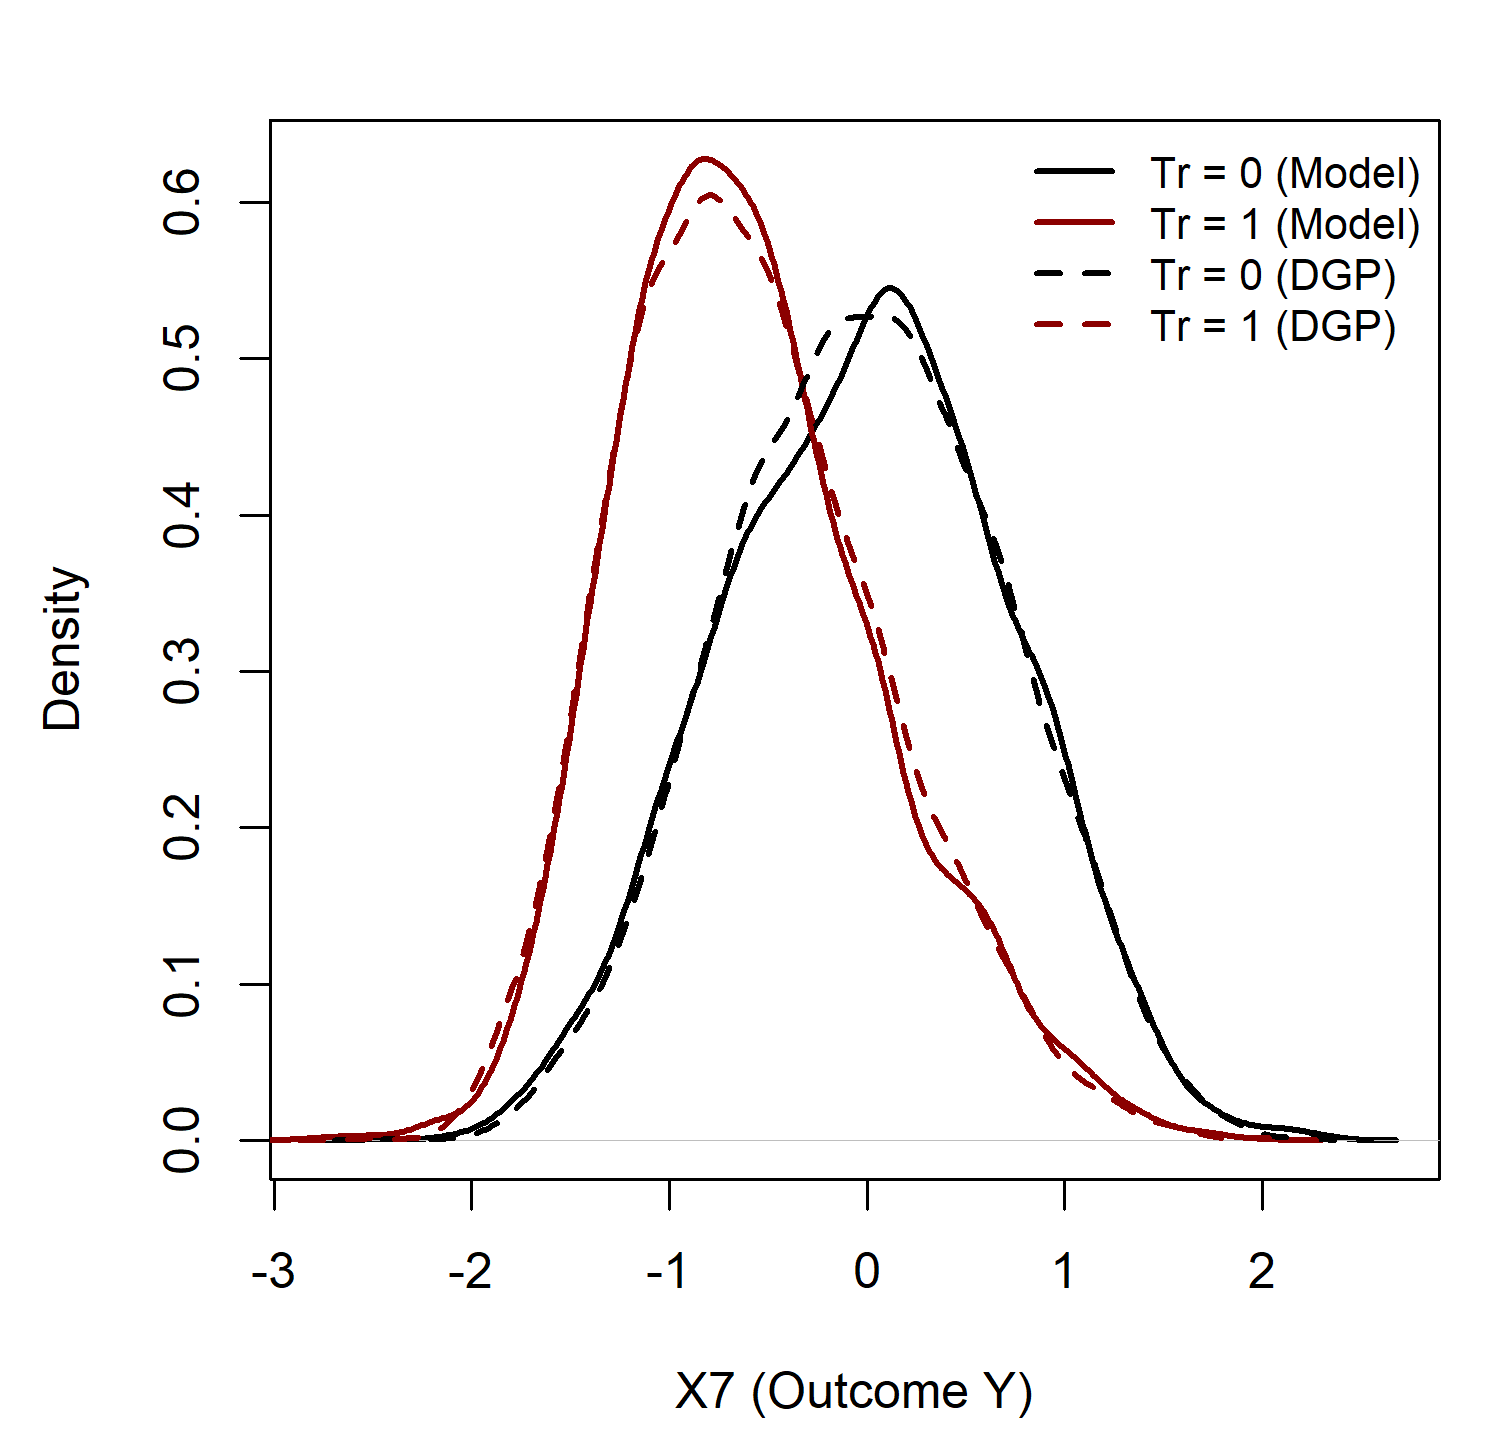
\includegraphics[width=0.45\textwidth]{img/results/observ_scenario2_X7_treatment_densities.png}
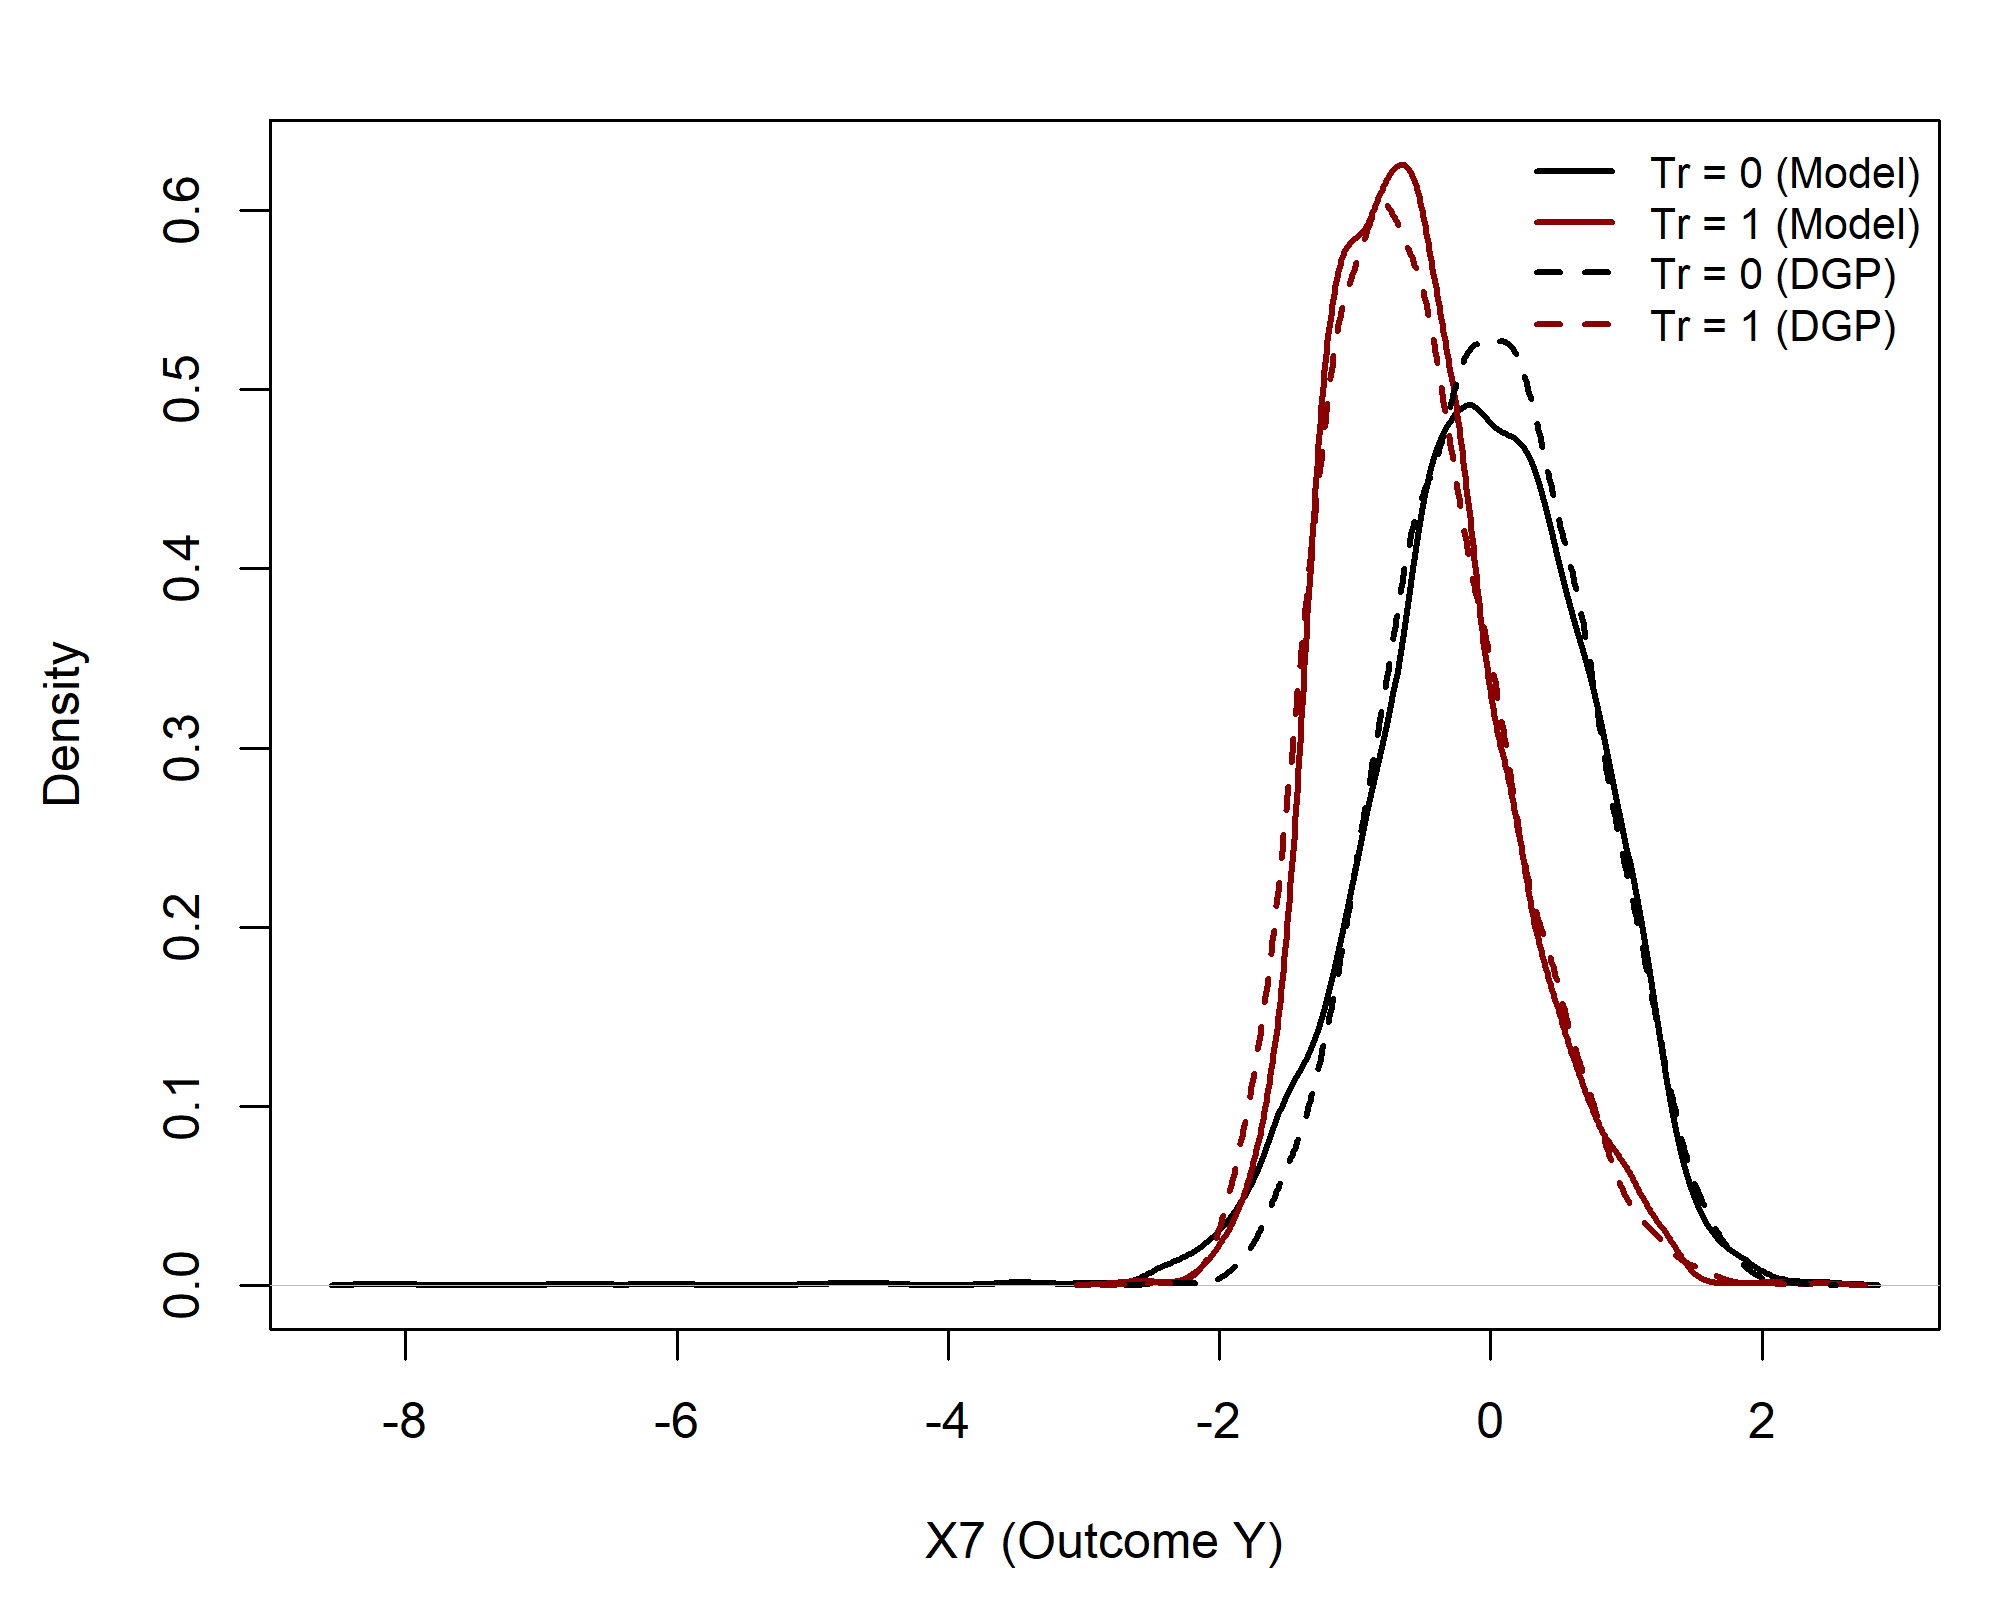
\includegraphics[width=0.45\textwidth]{img/results/rct_scenario2_X7_treatment_densities.png}
\caption{Distributions of the outcome variable ($X_7=Y$) under treatment and control interventions for Scenario~4.2, which includes a direct treatment effect but no interaction effects. This plot provides a higher-resolution view of the $X_7$ panels under do($X_4 = 0$) and do($X_4 = 1$) from Figure~\ref{fig:scenario2_sampling_distributions_vertical}. Left: Observational; Right: RCT setting.}
\label{fig:scenario2_outcome_distributions}
\end{figure}






\begin{figure}[htbp]
\centering
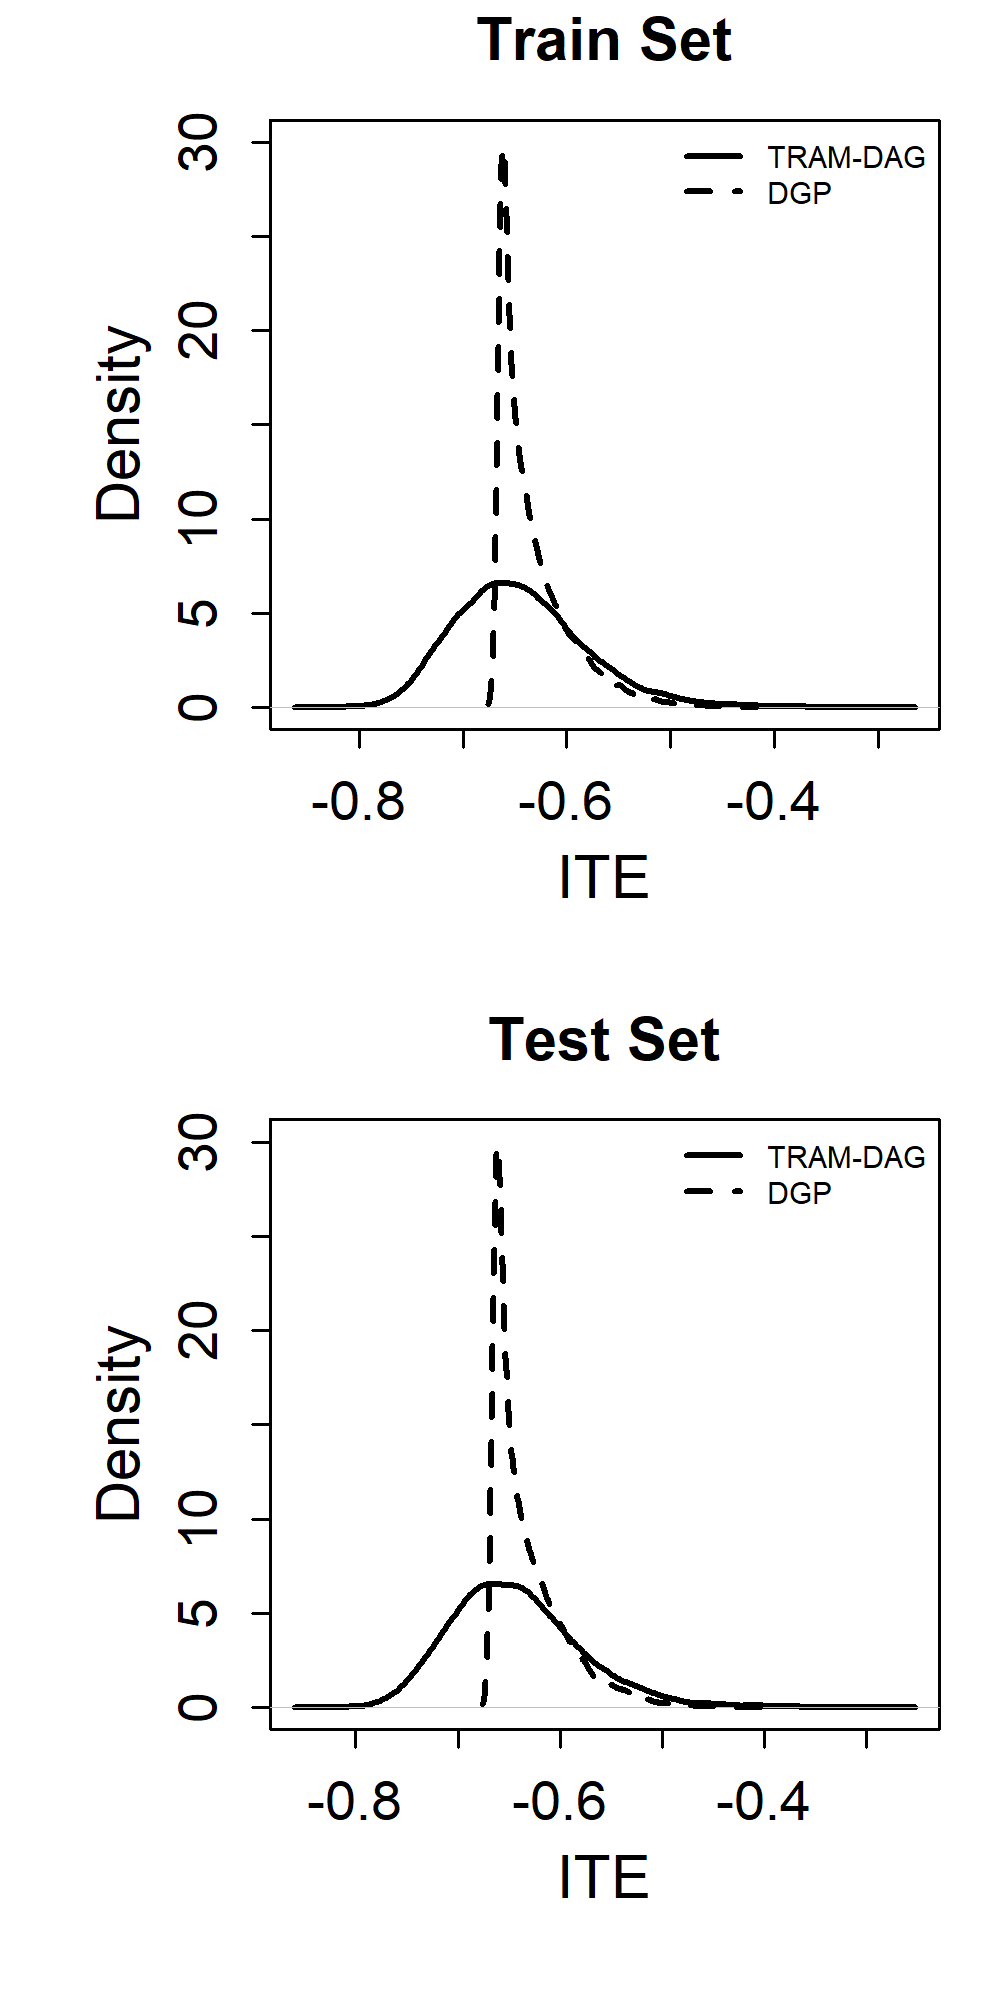
\includegraphics[width=0.33\textwidth]{img/results/observ_scenario2_ITE_densities_train_test.png}
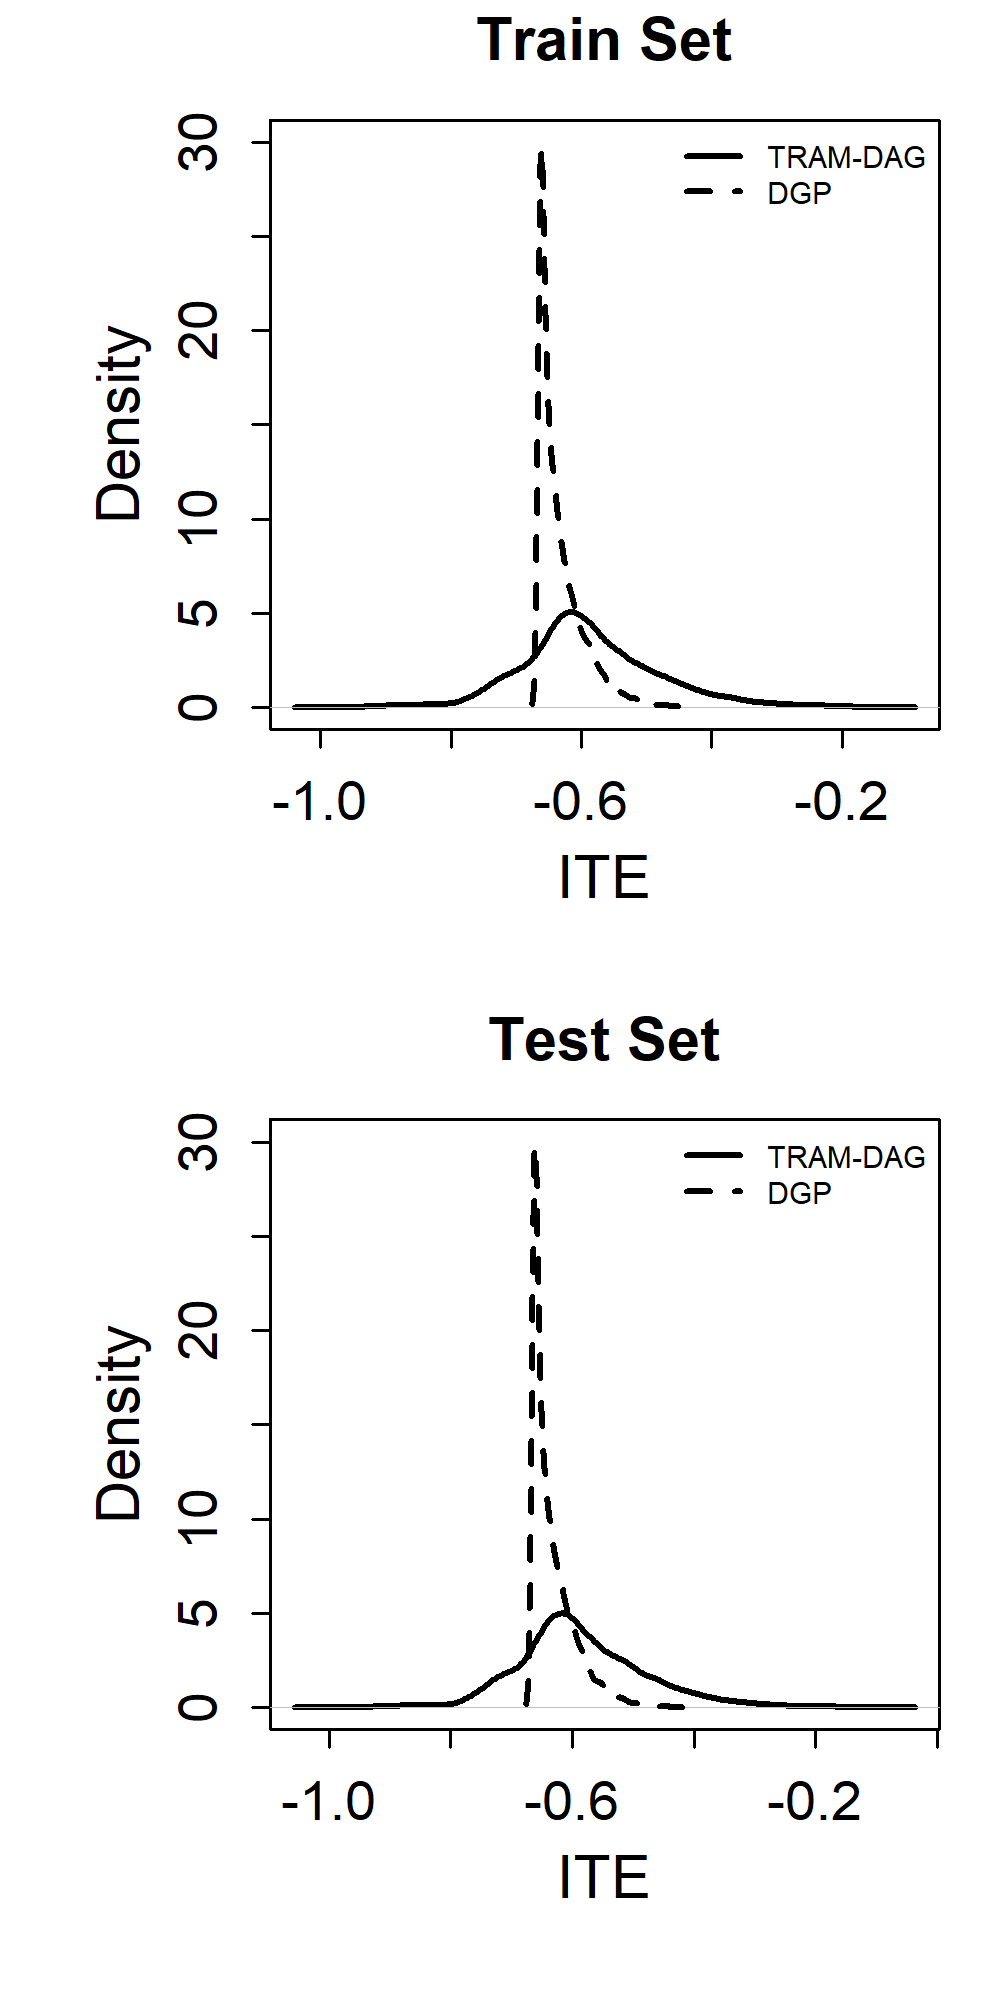
\includegraphics[width=0.33\textwidth]{img/results/rct_scenario2_ITE_densities_train_test.png}
\vspace{-17pt}
\caption{Densities of estimated ITEs compared to the true ITEs in the training and test datasets for Scenario~4.2, which includes a direct treatment effect but no interaction effects. Left: Observational; Right: RCT setting.}
\label{fig:scenario2_ite_densities_train_test}
\end{figure}






\begin{figure}[htbp]
\centering
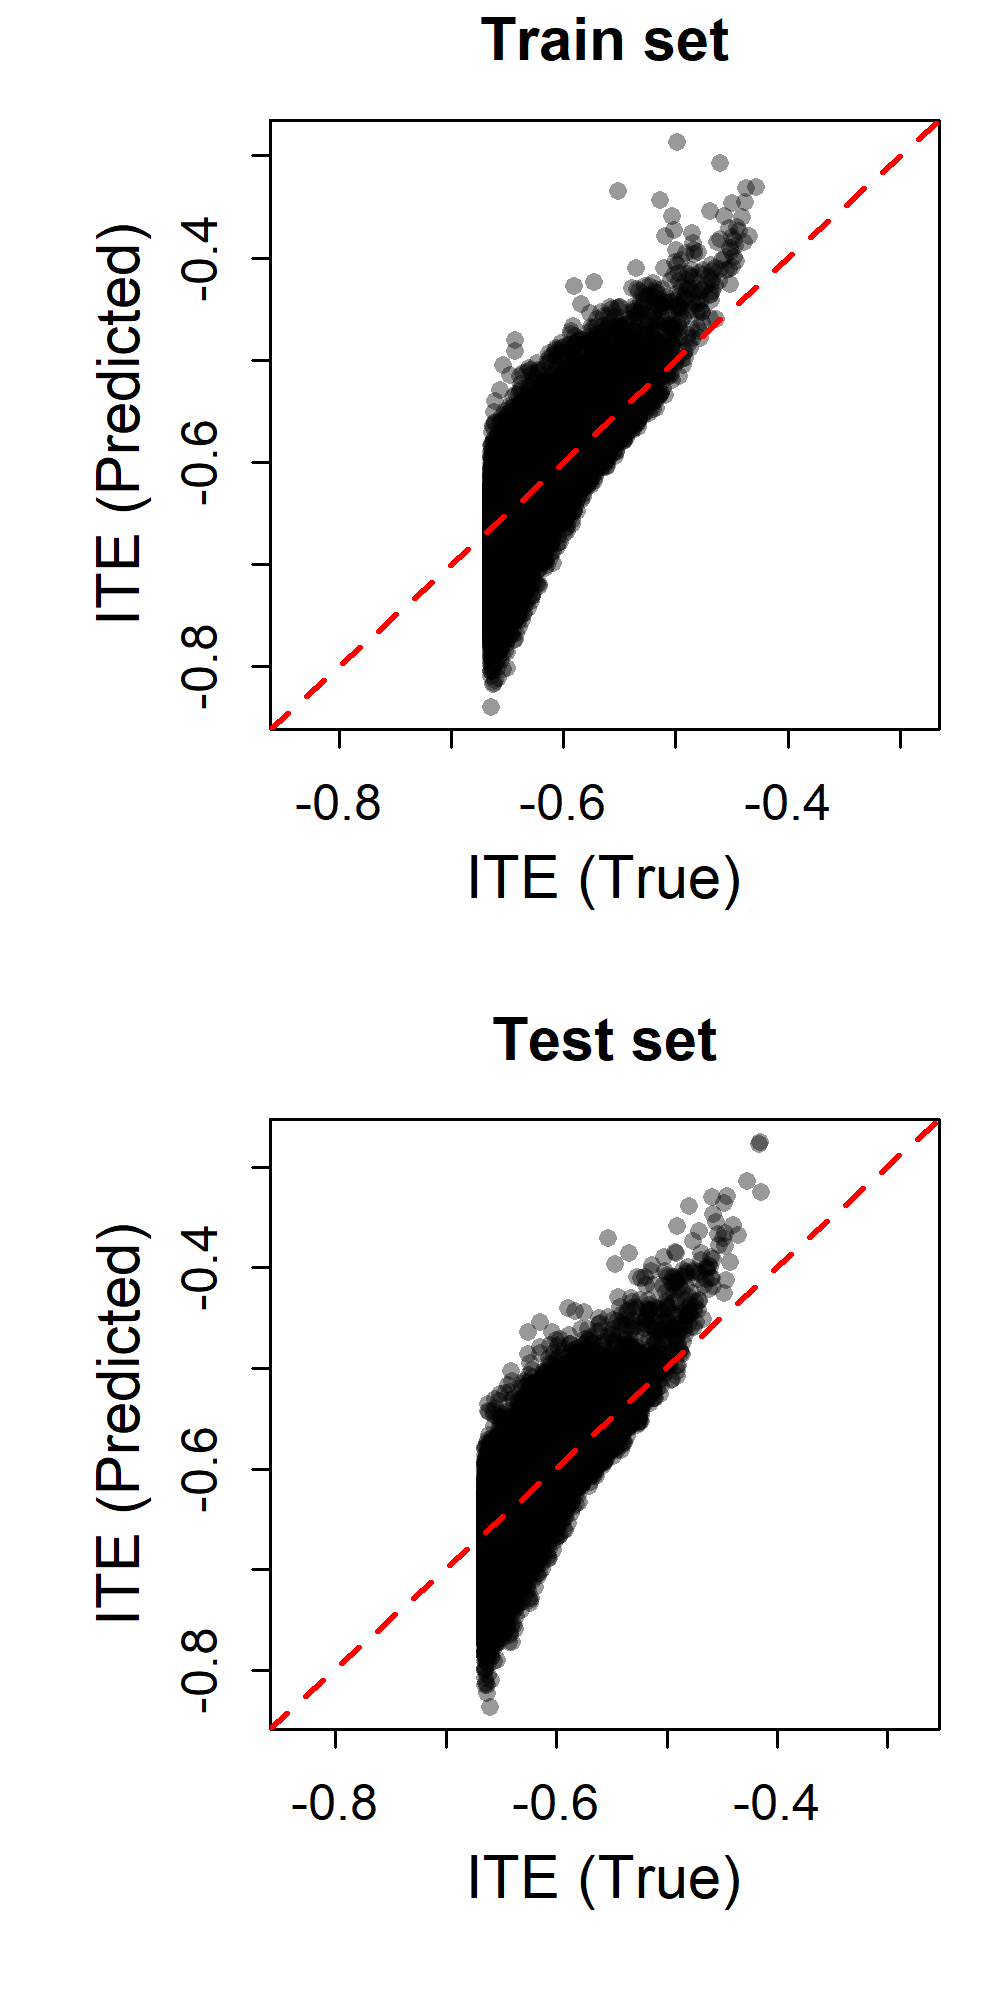
\includegraphics[width=0.33\textwidth]{img/results/observ_scenario2_ITE_scatter_train_test.png}
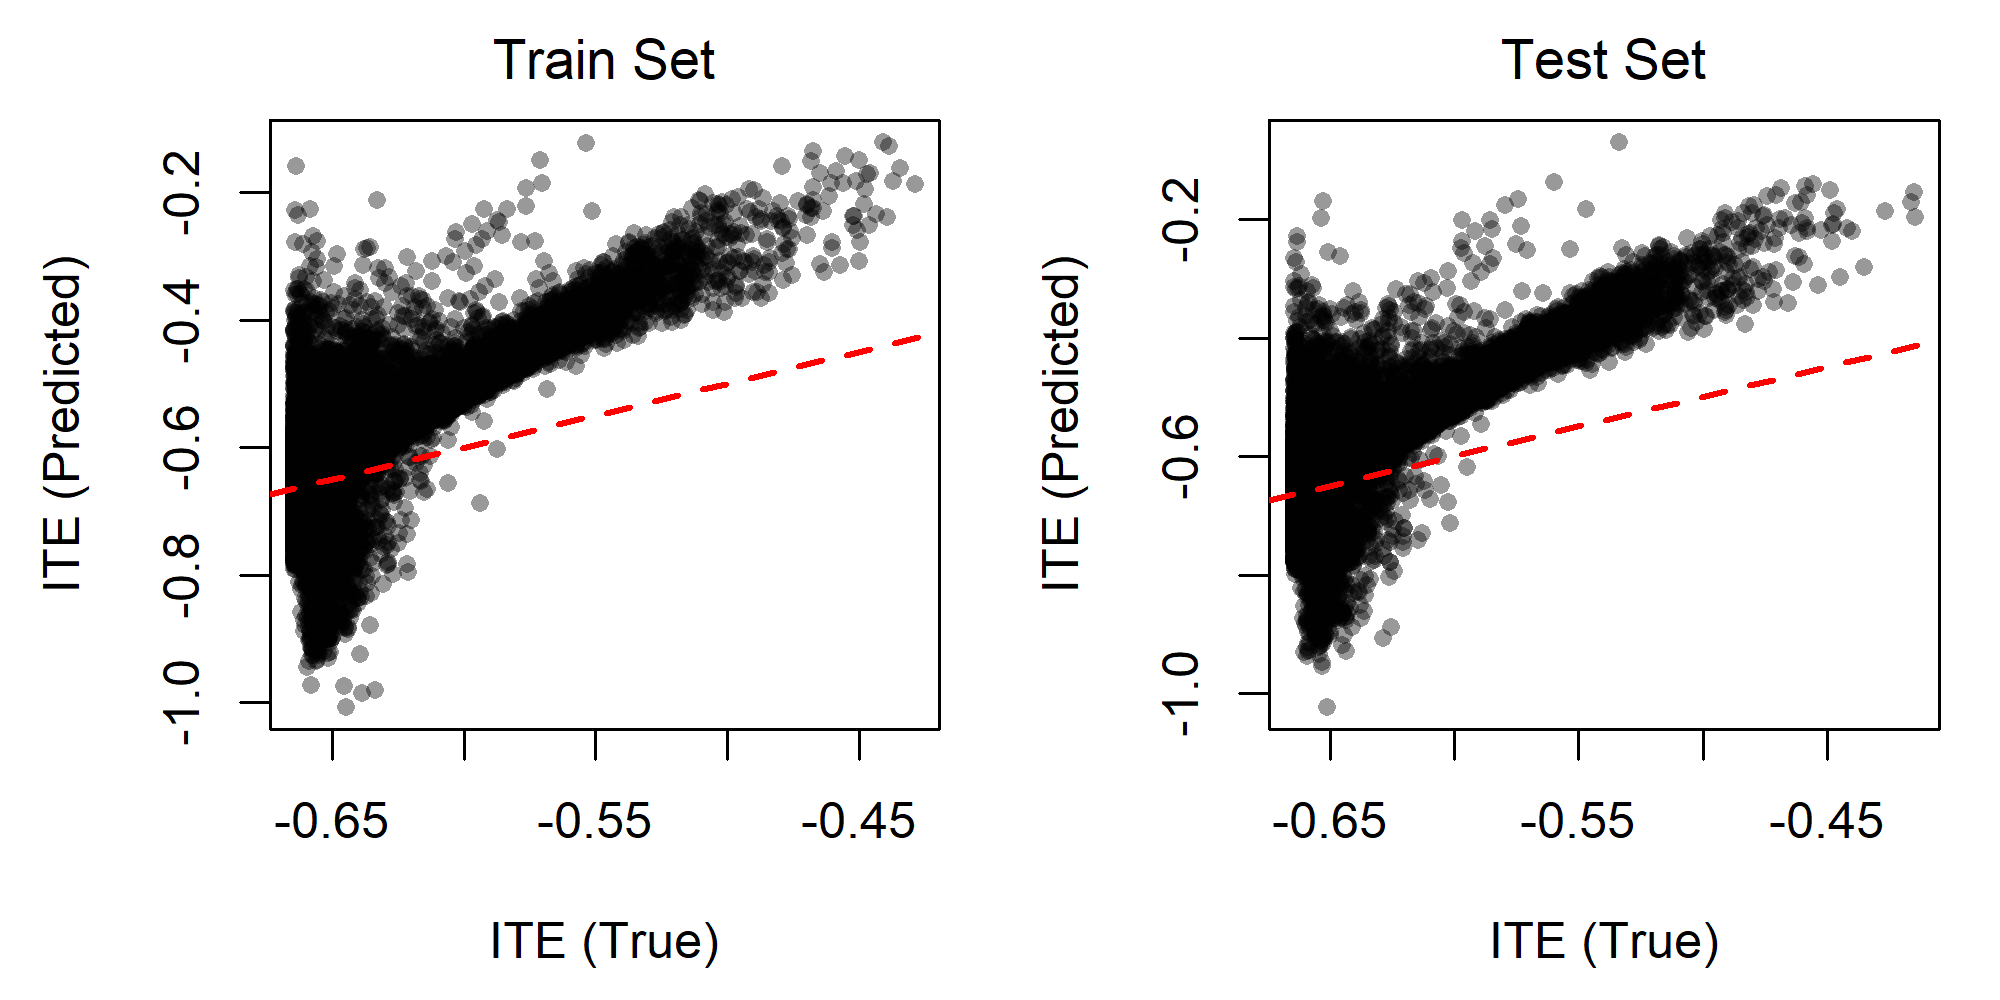
\includegraphics[width=0.33\textwidth]{img/results/rct_scenario2_ITE_scatter_train_test.png}
\vspace{-17pt}
\caption{Scatterplots of estimated ITEs compared to the true ITEs in the training and test datasets for Scenario~4.2, which includes a direct treatment effect but no interaction effects. Left: Observational; Right: RCT setting.}
\label{fig:scenario2_ite_scatter_train_test}
\end{figure}




\begin{figure}[htbp]
\centering
\includegraphics[width=0.8\textwidth]{img/results/observ_scenario2_ITE_ATE.png}
\vspace{-15pt}
\caption{ITE-ATE plot for Scenario~4.2 in the observational setting, which includes a direct treatment effect but no interaction effects. Individuals are grouped into bins based on their estimated ITEs, and in each bin, the ATE is computed as the difference in medians of the observed outcomes under treatment and control. The 95\% bootstrap confidence intervals indicate uncertainty.}
\label{fig:observ_scenario2_ite_ATE}
\end{figure}



\begin{figure}[htbp]
\centering
\includegraphics[width=0.8\textwidth]{img/results/rct_scenario2_ITE_ATE.png}
\vspace{-15pt}
\caption{ITE-ATE plot for Scenario~4.2 in the RCT setting, which includes a direct treatment effect but no interaction effects. Individuals are grouped into bins based on their estimated ITEs, and in each bin, the ATE is computed as the difference in medians of the observed outcomes under treatment and control. The 95\% bootstrap confidence intervals indicate uncertainty.}
\label{fig:rct_scenario2_ite_ATE}
\end{figure}



% enforce that starts after all floats have been displayed
\FloatBarrier

\textbf{Discussion of Scenario~4.2:} In Scenario~4.2, where no explicit interaction effects were present, ITE estimation was poor. Even though the TRAM-DAG could accurately reproduce observational and interventional distributions (see Figures~\ref{fig:scenario2_sampling_distributions_vertical} and~\ref{fig:scenario2_outcome_distributions}), the resulting ITEs could not be accurately determined (see Figures~\ref{fig:scenario2_ite_densities_train_test} and~\ref{fig:scenario2_ite_scatter_train_test}). This aligns with our discovery in Experiment~3 (Section~\ref{ch:experiment3}) that when true heterogeneity is weak, models tended to estimate too large heterogeneity, as shown, for example, in Figure \ref{fig:small_interaction_tuned_rf_tlearner} with the T-learner tuned random forest.

\medskip

What might be surprising in Scenario~4.2 is the presence of heterogeneity (variation in true ITEs), despite the absence of explicitly specified treatment-covariate interactions in the data-generating process. As shown in Figure~\ref{fig:scenario2_ite_distribution_dgp}, one might expect constant ITEs across individuals -- equal to the ATE -- given the model's additivity on the log-odds scale (Equation~\ref{eq:outcome_dgp}). However, as described by \citet{hoogland2021}, such heterogeneity arises because a constant treatment effect on the log-odds scale does not translate into a constant effect on a different scale, such as the probability scale. This phenomenon results from the nonlinearity of the inverse-link function (e.g., $\text{logit}^{-1}$), which transforms additive effects in the linear predictor into non-additive effects on the outcome scale. As they point out, the same shift induced by the treatment on the log-odds scale leads to different absolute risk reductions depending on the outcome risk under the control treatment. In other words, even with a homogeneous effect on the linear predictor, variation in covariates $\mathbf{X}$ leads to different treatment effects on the probability scale.

This would not have occurred under a linear model where the transformation function $h$ is the identity. In that case, the ITE would simplify as follows:

\begin{equation}
\text{ITE} = \mathbb{E}[Y(1)] - \mathbb{E}[Y(0)] = (\beta_0 + \beta_t + \boldsymbol{\beta}_x^\top \mathbf{X} + \epsilon) - (\beta_0 + \boldsymbol{\beta}_x^\top \mathbf{X} + \epsilon) = \beta_t
\label{eq:ITE_LM}
\end{equation}

In Equation~\ref{eq:ITE_LM}, the ITE is constant and equal to the treatment coefficient $\beta_t$, independent of the covariates or the noise term, which both cancel out.

In contrast, under a nonlinear model, such as the logistic transformation model with a nonlinear intercept function used in this experiment, the ITE becomes:

\begin{equation}
\text{ITE} = \mathbb{E}[h^{-1}(Z + \beta_t + \boldsymbol{\beta}_x^\top \mathbf{X})] - \mathbb{E}[h^{-1}(Z + \boldsymbol{\beta}_x^\top \mathbf{X})]
\end{equation}

Since $h^{-1}$ is nonlinear, the difference depends on the covariate profile $\mathbf{X}$ and on the noise term $Z$, even though the treatment effect $\beta_t$ is additive in the linear predictor, i.e., on the log-odds scale. It may therefore be worth thinking about whether analyzing the ITE on a scale where the effect is constant offers any advantages.

\medskip


% Maybe also related to this phenomenon, although not directly in the context of ITEs, is the concept of noncollapsibility, as discussed by \citet{dandl2025}. Noncollapsibility refers to the case when the treatment effect estimated from a marginal model (i.e., without covariates) does not correspond to the marginal effect that is obtained by averaging conditional treatment effects (i.e., adjusted for prognostic covariates) over the covariate distribution \citet{aalen2015}. Hence, treatment effects from two conditional models that use different sets of covariates for adjustment are not directly comparable if the model is noncollapsible. \citet{dandl2025} proposed a solution based on nonparanormal models \citep{liu2009, klein2022} to estimate a marginal treatment effect, while maintaining comparability (unaffected by covariates) and gaining from increased precision by adjusting for prognostic factors. Whether and how such an approach could be applied to ITE estimation is not explored further in this thesis.



\clearpage 



\subsubsection{Scenario 4.3: No direct effect, but with interaction effects} \label{sec:exp4_sc3}

\begin{figure}[H]
\centering
\includegraphics[width=0.85\textwidth]{img/exp4_dag_3.png}
\caption{DAGs for Scenario~4.3, which includes no direct effect of the treatment on the outcome, but interaction effects with covariates $X_2$ and $X_3$. Left: Observational; Right: RCT setting.}
\label{fig:ite_dag_observational_3}
\end{figure}

Scenario~4.3 includes no direct effect of the treatment on the outcome, but does include interaction effects between the treatment and covariates $X_2$ and $X_3$. Compared to Scenario~4.1 (Section~\ref{sec:exp4_sc1}), removing the direct effect results in a more centered ITE distribution, as shown in Figure~\ref{fig:scenario3_ite_distribution_dgp}. In the test set of the RCT setting, the ATE measured as the difference in means was -0.048, with a 95\% Wald confidence interval from -0.068 to -0.028. Note that the ATE in terms of difference in means cannot be directly compared to the ATE based on difference in medians.




\begin{table}[htbp]
\centering
\small
\caption{Scenario~4.3, without a direct treatment effect but including interaction effects: Comparison of ATE measures across train and test sets for the observational and RCT setting.  $\text{Y}_\text{observed}^{(\text{Tr})}$ denotes the observed outcome under the treatment ($\text{Tr}$) actually received. Estimates based on these observed outcomes (means and medians) are provided only for the RCT setting, as the observational setting is confounded. The true ITEs ($\text{ITE}_\text{true}$) were calculated for each individual based on the data-generating process. In contrast, the estimated ITEs ($\text{ITE}_\text{estimated}$) were obtained from the TRAM-DAG trained on observed data. The estimated ATE from $\text{mean}(\text{ITE}_\text{estimated})$ can be directly compared to the true $\text{mean}(\text{ITE}_\text{true})$, whereas comparisons to empirical ATEs from observed outcome differences should be interpreted with caution. All ITEs were computed as quantile treatment effects (QTEs) based on the median of the potential outcome distributions, as defined in Equation~\ref{eq:qte}.}
\label{tab:scenario3_ate_comparison}
\begin{tabular}{l c c c c}
\toprule
\textbf{Measure} & \multicolumn{2}{c}{\textbf{Observational}} & \multicolumn{2}{c}{\textbf{RCT}} \\
\cmidrule(lr){2-3} \cmidrule(lr){4-5}
 & \textbf{Train} & \textbf{Test} & \textbf{Train} & \textbf{Test} \\
\midrule
ATE as $\text{mean}(\text{Y}_\text{observed}^{(1)}) - \text{mean}(\text{Y}_\text{observed}^{(0)})$ 
& NA & NA 
& -0.048 
& -0.048 \\

ATE as $\text{median}(\text{Y}_\text{observed}^{(1)}) - \text{median}(\text{Y}_\text{observed}^{(0)})$  
& NA & NA 
& -0.048 
& -0.059 \\

ATE as mean(ITE$_\text{true}$)  
& -0.065 
& -0.068 
& -0.065 
& -0.068 \\

ATE as mean(ITE$_\text{estimated}$) 
& -0.059 
& -0.061 
& -0.051 
& -0.053 \\
\bottomrule
\end{tabular}
\end{table}


% \begin{table}[htbp]
% \centering
% \small
% \caption{Scenario (3), without direct treatment effect but including interaction effects: Comparison of ATE measures across train and test sets for the observational and RCT setting.}
% \label{tab:scenario3_ate_comparison_old}
% \begin{tabular}{l c c c c}
% \toprule
% \textbf{Measure} & \multicolumn{2}{c}{\textbf{Observational}} & \multicolumn{2}{c}{\textbf{RCT}} \\
% \cmidrule(lr){2-3} \cmidrule(lr){4-5}
%  & \textbf{Train} & \textbf{Test} & \textbf{Train} & \textbf{Test} \\
% \midrule
% ATE as $\text{mean}(\text{Y}_\text{observed}^{(1)}) - \text{mean}(\text{Y}_\text{observed}^{(0)})$ & NA & NA & round(rct_scenario3$dev_ATE_observed_Y_mean_diff, 3) & round(rct_scenario3$val_ATE_observed_Y_mean_diff, 3) \\
% ATE as $\text{median}(\text{Y}_\text{observed}^{(1)}) - \text{median}(\text{Y}_\text{observed}^{(0)})$ & NA & NA & round(rct_scenario3$dev_ATE_observed_Y_median_diff, 3) & round(rct_scenario3$val_ATE_observed_Y_median_diff, 3) \\
% ATE as mean(ITE$_\text{true}$)  & round(observ_scenario3$dev_ITE_median_average, 3) & round(observ_scenario3$val_ITE_median_average, 3) & round(rct_scenario3$dev_ITE_median_average, 3) & round(rct_scenario3$val_ITE_median_average, 3) \\
% ATE as mean(ITE$_\text{estimated}$) & round(observ_scenario3$dev_ITE_median_pred_average, 3) & round(observ_scenario3$val_ITE_median_pred_average, 3) & round(rct_scenario3$dev_ITE_median_pred_average, 3) & round(rct_scenario3$val_ITE_median_pred_average, 3) \\
% \bottomrule
% \end{tabular}
% \end{table}
% 


\begin{figure}[htbp]
\centering
\includegraphics[width=0.7\textwidth]{img/results/observ_scenario3_ite_distribution_dgp.png}
\caption{True ITE distribution resulting from the DGP for Scenario~4.3, which includes interaction effects but no direct treatment effect. The true ITEs are identical in the observational and RCT settings, since they are based on the potential outcomes under both treatment allocations.}
\label{fig:scenario3_ite_distribution_dgp}
\end{figure}



\begin{figure}[htbp]
\centering
\includegraphics[width=0.45\textwidth]{img/results/observ_scenario3_sampling_distributions_vertical.png}
\includegraphics[width=0.45\textwidth]{img/results/rct_scenario3_sampling_distributions_vertical.png}
\caption{Marginal distributions of variables from the DGP and from samples generated by the fitted TRAM-DAG for Scenario~4.3, which includes interaction effects but no direct treatment effect. The distributions are shown as observed (Obs), under control intervention do($X_4 = 0$), and under treatment intervention do($X_4 = 1$). Left: Observational; Right: RCT setting.}
\label{fig:scenario3_sampling_distributions_vertical}
\end{figure}



\begin{figure}[htbp]
\centering
\includegraphics[width=0.45\textwidth]{img/results/observ_scenario3_X7_treatment_densities.png}
\includegraphics[width=0.45\textwidth]{img/results/rct_scenario3_X7_treatment_densities.png}
\caption{Distributions of the outcome variable ($X_7=Y$) under treatment and control interventions for Scenario~4.3, which includes interaction effects but no direct treatment effect. This plot provides a higher resolution view of the $X_7$ panels under do($X_4 = 0$) and do($X_4 = 1$) from Figure~\ref{fig:scenario3_sampling_distributions_vertical}. Left: Observational; Right: RCT setting.}
\label{fig:scenario3_outcome_distributions}
\end{figure}




\begin{figure}[htbp]
\centering
\includegraphics[width=0.33\textwidth]{img/results/observ_scenario3_ITE_densities_train_test.png}
\includegraphics[width=0.33\textwidth]{img/results/rct_scenario3_ITE_densities_train_test.png}
\vspace{-17pt}
\caption{Densities of estimated ITEs compared to the true ITEs in the training and test datasets for Scenario~4.3, which includes interaction effects but no direct treatment effect. Left: Observational; Right: RCT setting.}
\label{fig:scenario3_ite_densities_train_test}
\end{figure}






\begin{figure}[htbp]
\centering
\includegraphics[width=0.33\textwidth]{img/results/observ_scenario3_ITE_scatter_train_test.png}
\includegraphics[width=0.33\textwidth]{img/results/rct_scenario3_ITE_scatter_train_test.png}
\vspace{-17pt}
\caption{Scatterplots of estimated ITEs compared to the true ITEs in the training and test datasets for Scenario~4.3, which includes interaction effects but no direct treatment effect. Left: Observational; Right: RCT setting.}
\label{fig:scenario3_ite_scatter_train_test}
\end{figure}




\begin{figure}[htbp]
\centering
\includegraphics[width=0.8\textwidth]{img/results/observ_scenario3_ITE_ATE.png}
\vspace{-15pt}
\caption{ITE-ATE plot for Scenario~4.3 in the observational setting, which includes interaction effects but no direct treatment effect. Individuals are grouped into bins based on the estimated ITE, and within each bin the ATE is computed as the difference in medians of the observed outcomes under treatment and control. 95\% bootstrap confidence intervals reflect the uncertainty.}
\label{fig:observ_scenario3_ite_ATE}
\end{figure}


\begin{figure}[htbp]
\centering
\includegraphics[width=0.8\textwidth]{img/results/rct_scenario3_ITE_ATE.png}
\vspace{-15pt}
\caption{ITE-ATE plot for Scenario~4.3 in the RCT setting, which includes interaction effects but no direct treatment effect. Individuals are grouped into bins based on the estimated ITE, and within each bin the ATE is computed as the difference in medians of the observed outcomes under treatment and control. 95\% bootstrap confidence intervals reflect the uncertainty.}
\label{fig:rct_scenario3_ite_ATE}
\end{figure}




% enforce that starts after all floats have been displayed
\FloatBarrier


\textbf{Discussion of Scenario~4.3:} In Scenario~4.3, which included interaction effects but no direct treatment effect, the TRAM-DAG could successfully estimate the ITE (similarly as in Scenario 4.1; Section~\ref{sec:exp4_sc1}). The scatterplots of estimated ITEs vs. true ITEs (Figure~\ref{fig:scenario3_ite_scatter_train_test}) showed good prediction accuracy.





%  --> the following will be used in Experiment 4 (methods)
% http://www.mit.edu/~vchern/papers/ch_iqr_ema.pdf estimate the quantile treatment effect (heterogeneous) with instrumental variables, it looks very similar to the TRAM-DAG approach: *This interpretation makes quantile analysis an interesting tool for describing and learning the structure of heterogeneous treatment effects and controlling for unobserved heterogeneity."

% https://www.rfberlin.com/wp-content/uploads/2024/12/24030.pdf good book/paper about instrumental variables, also talks about potential outcomes (but i should maybe not go too much into detial)

% - maybe include somewhere the discussion about the difference between discrimination and claibraion:
% https://bavodc.github.io/websiteCalibrationCurves/articles/CalibrationCurves.html




% An example could be the psychological condition of a patient which might also affect how the treatment works, this is not a confounder but an effect modifier, and i would assume that this variable is rarely recorede or measured.



% enforce that starts after all floats have been displayed
\FloatBarrier


\subsection{Discussion of Experiment 4} \label{sec:disc_experiment4}


TRAM-DAGs provided unbiased estimates of ITEs in Scenario 1 (Section~\ref{sec:exp4_sc1}) and Scenario 3 (Section~\ref{sec:exp4_sc3}), where heterogeneity of treatment effects was strong. This supports our claim that TRAM-DAGs can effectively be unbiased ITE estimation in a complex scenario, if the DAG is fully observed and heterogeneity is strong.



% We analyzed ITE estimation under an observational setting (confounded) and under an RCT setting (randomized treatment allocation) in three different scenarios: direct and interaction treatment effect, only direct but no interaction effect, and no direct but with interaction effect. 
% 
% The TRAM-DAG could successfully estimate the ITE in Scenario 1 and Scenario 3 where interaction effects were present. There was no notable difference between the observational and RCT settings. Scatterplots of estimated ITEs vs. true ITEs showed good prediction accuracy (see Figures \ref{fig:scenario1_ite_scatter_train_test} and \ref{fig:scenario3_ite_scatter_train_test}). Also the ATE based on the mean of estimated ITEs was close to the ATE based on true ITEs in both scenarios (see Tables \ref{tab:scenario1_ate_comparison} and \ref{tab:scenario3_ate_comparison}). These results highlight TRAM-DAG's ability to compute counterfactuals for mediators and to estimate individualized treatment effects even in relatively complex DAG structures.
% 
% 
% 
% In Scenario 2, where no explicit interaction effects were present, ITE estimation was poor. This aligns with our discovery in Experiment 3 that when true heterogeneity is weak, models tended to estimate too large heterogeneity, as e.g. shown in Figure \ref{fig:small_interaction_tuned_rf_tlearner} with the T-learner tuned random forest.
% 
% \medskip
% 
% What might be surprising in Scenario 2 is the presence of heterogeneity (true ITEs), despite the absence of explicitly specified interaction terms in the data-generating process. As shown in Figure~\ref{fig:scenario2_ite_distribution_dgp}, one might have expected the ITEs to be constant across individuals -- equal to the ATE -- given the model's additivity on the log-odds scale. However, as described by \citet{hoogland2021}, such heterogeneity arises because a constant treatment effect on the log-odds scale does not translate into a constant effect on a different scale, such as the probability scale. This phenomenon results from the nonlinearity of the inverse-link function (e.g., $\text{logit}^{-1}$), which transforms additive effects in the linear predictor into non-additive effects on the outcome scale. As the authors point out, the same shift induced by the treatment on the log-odds scale leads to different absolute risk reductions depending on the outcome risk under the control treatment. In other words, even with a homogeneous effect on the linear predictor, variation in covariates $\mathbf{X}$ leads to different treatment effects on the probability scale.
% 
% This would not have occurred under a linear model where the transformation function $h$ is the identity. In that case, the ITE would simplify as follows:
% 
% \begin{equation}
% \text{ITE} = \mathbb{E}[Y(1)] - \mathbb{E}[Y(0)] = (\beta_0 + \beta_t + \boldsymbol{\beta}_x^\top \mathbf{X} + \epsilon) - (\beta_0 + \boldsymbol{\beta}_x^\top \mathbf{X} + \epsilon) = \beta_t
% \end{equation}
% 
% Here, the ITE is constant and equal to the treatment coefficient, independent of the covariates or the noise term, which cancels out.
% 
% In contrast, under a nonlinear model, such as the logistic transformation model with a nonlinear intercept function used in this experiment, the ITE becomes:
% 
% \begin{equation}
% \text{ITE} = \mathbb{E}[h^{-1}(Z + \beta_t + \boldsymbol{\beta}_x^\top \mathbf{X})] - \mathbb{E}[h^{-1}(Z + \boldsymbol{\beta}_x^\top \mathbf{X})]
% \end{equation}
% 
% Since $h^{-1}$ is nonlinear, the difference depends on the covariate profile $\mathbf{X}$ and on the noise term $Z$, even though the treatment effect $\beta_t$ is additive in the linear predictor, i.e., on the log-odds scale. It may therefore be worth thinking about whether analyzing the ITE on a scale where the effect is constant offers any advantages.
% 
% \medskip
% 
% 
% Maybe also related to this phenomenon, although not directly in the context of ITEs, is the concept of noncollapsibility, as discussed by \citet{dandl2025}. Noncollapsibility refers to the case when the treatment effect estimated from a marginal model (i.e., without covariates) does not correspond to the marginal effect that is obtained by averaging conditional treatment effects (i.e., adjusted for prognostic covariates) over the covariate distribution \citet{aalen2015}. Hence, treatment effects from two conditional models that use different sets of covariates for adjustment are not directly comparable if the model is noncollapsible. \citet{dandl2025} proposed a solution based on nonparanormal models \citep{liu2009, klein2022} to estimate a marginal treatment effect, while maintaining comparability (unaffected by covariates) and gaining from increased precision by adjusting for prognostic factors. Whether and how such an approach could be applied to ITE estimation is not explored further in this thesis.


% Maybe also related to this phenomenon, although not in the context of ITEs, might be the concept of non-collapsibility, as discussed by \citet{dandl2025}. Non-collapsibility refers to the case when the treatment effect from a marginal model does not correspond to the marginal effect that is obtained from a conditional treatment effect (i.e. adjusted for prognostic covariates) by averaging over the prognostic variables. Hence, treatment effects from two conditional models that used different sets of covariate for adjustments are not comparable if a model is non-collapsible. The authors proposed a solution based on nonparanomrmal models (\citealp{{liu2009}; \citealp{klein2022}) to estimate a marginal treatment effect, while maintaining comparability (unaffected by covariates) and gaining from increased precision by adjusting for prognostic factors. However, if and how this would translate to ITE estimation goes beyond the scope of this thesis.

% What might be surprising is that in Scenario 2 where we dont have explicitly included interaction terms in the data generating process, there is still some heterogeneity in the treatment effect, as shown in Figure \ref{fig:scenario2_ite_distribution_dgp}. One might expect that the ITE is constant across all individuals in such a case, and equal to the ATE. 
% 
% \citep{hoogland2021} chapter 4.1 well described this phenomenon of non-additivity leaving the log-odds scale.
% % the problem with non-additivity is perffectly described in Hoogland "A tutorial on individualized treatment effect prediction from randomized trials with a binary endpoint
% 
% However since we used a non linear transformatino function as intercept in the data generating process (as would likely be the case in a real world setting), the treatment effect is not constant across all individuals (which should correspond to the ATE). When a linear transformation function would be applied (as for example a linear regression is specified, where the latent noise distribution would be the standard normal and the transformation function would be linear) then the noise term cancels out when calculating the ITE, leading to a constant ITE when no interactions are present: $\text{ITE} = \text{E}[Y(1)] -\text{E}[Y(0)] = (\beta_0 + \beta_t 1 + \beta_x X + \epsilon) - (\beta_0 + \beta_t 0 + \beta_x X + \epsilon) = \beta_t$.
% 
% In a model with nonlinear transformation, as in this experiment, the noise term does not cancel out anymore leading to different ITEs for patients with different characteristics.
% 
% \begin{equation}
% \text{ITE} = \text{E}[Y(1) - Y(0)] = \text{E}[h^{-1}(Z + \beta_t 1 + \beta_x X)] - \text{E}[h^{-1}(Z + \beta_t 0 + \beta_x X)] 
% \end{equation}
% 
% where $h$ is the nonlinear transformation function, $Z$ is the latent noise term, $\beta_t$ is the direct treatment effect and $\beta_x$ are the coefficients of the covariates. The state of the covariates $X$ alters the position on the transformation function and thereby affects the difference between the two terms. If the transformation was fixed to be linear, the difference would be constant independent of the state of the covariates $X$. 

% (This also has to do with non-collapsibility as discussed by susanne and torsten , also check Beates Mail 21.06.2025, and chatgpt discussion)



% cite susanne and torsten paper: https://arxiv.org/abs/2503.01657









